\documentclass{skripsi}

% -------------------------------------------------------------------
% METADATA DOKUMEN SKRIPSI
% -------------------------------------------------------------------
\judulindonesia{Strategi Pemasaran Rumah Makan Nasi Gerilya pada Platform GrabFood untuk Meningkatkan Penjualan Berdasarkan Analisis SWOT}
\judulindonesiacapitalize{Strategi Pemasaran Rumah Makan Nasi Gerilya \\ pada Platform GrabFood untuk Meningkatkan \\ Penjualan Berdasarkan Analisis SWOT}
\judulindonesiacapslock{STRATEGI PEMASARAN RUMAH MAKAN NASI GERILYA \\ PADA PLATFORM GRABFOOD UNTUK MENINGKATKAN \\ PENJUALAN BERDASARKAN ANALISIS SWOT}

\judulinggris{Marketing Strategy of Nasi Gerilya Restaurant on the GrabFood Platform to Increase Sales Based on SWOT Analysis}
\judulinggriscapitalize{Marketing Strategy of Nasi Gerilya Restaurant \\ on the GrabFood Platform to Increase Sales \\ Based on SWOT Analysis}
\judulinggriscapslock{MARKETING STRATEGY OF NASI GERILYA RESTAURANT \\ ON THE GRABFOOD PLATFORM TO INCREASE SALES \\ BASED ON SWOT ANALYSIS}

\author{Marsia Br Pelawi}
\nim{220502068}
\programstudi{Strata 1 Manajemen}
\fakultas{Ekonomi dan Bisnis}
\universitas{Universitas Sumatera Utara}
\tahun{2026}
\kota{Medan}
\tanggalpengesahan{06 Mei 2026}
\labelpenandatangan{Peneliti}
\namapenandatangan{Marsia Br Pelawi}
\logopath{resource/01-brand/logo-usu.png} % Path logo universitas


% Tambahkan .bib file untuk daftar pustaka
\addbibresource{referensi.bib}
\usepackage{pgfplots}
\usepackage{diagbox}
\usepackage{tikz}
\usetikzlibrary{tikzmark,calc}
\usepackage{float}
\pgfplotsset{compat=1.18}

\begin{document}

% -------------------------------------------------------------------
% BAGIAN AWAL (FRONTMATTER)
% -------------------------------------------------------------------
\pagenumbering{roman} % Halaman angka romawi kecil (i, ii, iii)
\pagestyle{plain} % Halaman diletakkan di bawah-tengah

\makecover

\abstrakindonesia{Rumah Makan Nasi Gerilya merupakan usaha nasi Padang di Kota Medan yang menggunakan GrabFood sebagai salah satu kanal penjualan utama, tetapi kondisi di lokasi penelitian menunjukkan penjualan yang belum stabil, pembelian ulang yang menurun, adanya keluhan pelanggan, serta tekanan persaingan dari merchant sejenis pada platform yang sama. Tujuan penelitian ini adalah mengidentifikasi faktor internal dan eksternal Rumah Makan Nasi Gerilya pada platform GrabFood serta merumuskan strategi pemasaran berdasarkan analisis SWOT untuk mendukung peningkatan penjualan. Penelitian dilakukan pada Rumah Makan Nasi Gerilya di Kota Medan dengan fokus pada aktivitas pemasaran melalui GrabFood. Pengumpulan data dilakukan melalui wawancara dengan pemilik, pegawai, pelanggan, dan informan pembanding, observasi platform GrabFood, wawancara pelanggan, dokumentasi usaha, ulasan pelanggan, serta studi pustaka. Hasil penelitian menunjukkan bahwa skor IFAS sebesar 2,50 dan skor EFAS sebesar 2,51 menempatkan Nasi Gerilya pada kondisi sedang dengan posisi Kuadran I, yaitu strategi agresif atau SO karena kekuatan internal dan peluang eksternal lebih dominan daripada kelemahan dan ancaman. Kekuatan utama usaha terletak pada cita rasa lauk, porsi besar, reputasi digital, alur pengecekan pesanan, dan respons keluhan, sedangkan kelemahan utama terdapat pada akurasi packing, antrean lintas kanal, update stok, persepsi harga, dan kejelasan deskripsi paket. Strategi alternatif yang dirumuskan meliputi strategi SO, WO, ST, dan WT, dengan prioritas pada perbaikan sistem antrean dan checklist packing, penguatan paket menu unggulan berbasis segmen, perbaikan tampilan digital dan menu digital, sinkronisasi promo dengan stok, kapasitas, HPP, dan margin, serta pemanfaatan stamp digital, database pelanggan, dan Flowie untuk mendorong pembelian ulang.}

\katakunciindonesia{strategi pemasaran, GrabFood, SWOT, UMKM kuliner, penjualan}


\begin{abstrak}
    \abstrakindonesiatext

    \katakunci{\katakunciindonesiatext}
\end{abstrak}

\abstrakinggris{Nasi Gerilya Restaurant is a Padang food business in Medan that uses GrabFood as one of its main sales channels, yet the situation at the research site shows unstable sales, a declining proportion of repeat purchases, customer complaints, and competitive pressure from similar merchants on the same platform. The purpose of this study is to identify the internal and external factors of Nasi Gerilya Restaurant on the GrabFood platform and to formulate marketing strategies based on SWOT analysis to support sales improvement. The research was conducted at Nasi Gerilya Restaurant in Medan, focusing on its marketing activities through GrabFood. Data were collected through interviews with the owner, employees, customers, and comparative informants, GrabFood platform observation, customer questionnaires, business documentation, customer reviews, and literature study. The results show that an IFAS score of 2.50 and an EFAS score of 2.51 place Nasi Gerilya in a moderate condition and in Quadrant I, namely an aggressive or SO strategy position, because internal strengths and external opportunities are more dominant than weaknesses and threats. The main strengths are strong food taste, large portions, digital reputation, an order-checking flow, and complaint response, while the main weaknesses are packing accuracy, cross-channel queues, stock updates, price perception, and unclear package descriptions. The alternative strategies formulated include SO, WO, ST, and WT strategies, with priorities on improving the queue system and packing checklist, strengthening segment-based hero menu packages, improving the digital storefront and digital menu, synchronizing promotions with stock, capacity, cost of goods sold, and margins, and utilizing digital stamps, customer databases, and Flowie to encourage repeat purchases.}

\katakunciinggris{marketing strategy, GrabFood, SWOT, culinary MSME, sales}


\begin{abstracteng}
    \abstrakinggristext

    \katakunci{\katakunciinggristext}
\end{abstracteng}

\begin{katapengantar}
    Segala puji syukur peneliti panjatkan kepada Tuhan Yesus Kristus atas kasih, berkat, dan penyertaan-Nya sehingga peneliti dapat menyelesaikan skripsi yang berjudul \textbf{"\judulindonesiatext"}. Tujuan penulisan skripsi ini adalah sebagai salah satu syarat untuk memperoleh gelar Sarjana Manajemen pada Program Studi S1 Manajemen, Fakultas Ekonomi dan Bisnis, Universitas Sumatera Utara.

    Pada kesempatan ini, peneliti mengucapkan terima kasih yang sebesar-besarnya kepada kedua \textbf{orang tua tercinta} yang telah membesarkan, mendidik, mendoakan, dan memberikan dukungan kepada peneliti. Selama proses penyusunan skripsi ini, peneliti menyadari banyak mendapat bantuan, bimbingan, dan dukungan dari berbagai pihak. Untuk itu, peneliti mengucapkan terima kasih sebesar-besarnya kepada:

    \begin{enumerate}
        \item Bapak Prof. Dr. Muryanto Amin, S.Sos., M.Si., selaku Rektor Universitas Sumatera Utara.
        \item Bapak Dr. Abdillah Arif Nasution, S.E., M.Si., Ak., C.A., QGIA, CHRS, selaku Dekan Fakultas Ekonomi dan Bisnis Universitas Sumatera Utara.
        \item Ibu Prof. Dr. Khaira Amalia Fachrudin, S.E., Ak., M.B.A., selaku Ketua Program Studi S1 Manajemen dan Bapak Muhammad Arif Lubis, S.E., M.Si., selaku Sekretaris Program Studi S1 Manajemen Fakultas Ekonomi dan Bisnis Universitas Sumatera Utara.
        \item Ibu Dr. Tetty Yuliaty, S.E., M.Si., selaku Dosen Pembimbing yang telah memberikan bimbingan, arahan, masukan, dan dukungan kepada peneliti dalam penyusunan skripsi ini.
        \item Ibu Prof. Dr. Arlina Nurbaity Lubis, S.E., M.B.A., selaku Dosen Penguji I yang telah memberikan masukan dan saran untuk penyempurnaan skripsi ini.
        \item Bapak Haryaji Catur Putera Hasman, S.E., M.Si., selaku Dosen Penguji II yang telah memberikan masukan dan saran untuk penyempurnaan skripsi ini.
        \item Seluruh dosen dan pegawai Fakultas Ekonomi dan Bisnis Universitas Sumatera Utara, khususnya Program Studi S1 Manajemen, yang telah memberikan ilmu, bantuan, dan pelayanan akademik kepada peneliti selama masa perkuliahan.
        \item Pemilik dan seluruh karyawan Rumah Makan Nasi Gerilya yang telah memberikan izin, waktu, informasi, dan bantuan selama proses penelitian.
        \item Adrian, selaku \textit{significant other}, yang selama 24/7 memberikan dukungan sepenuhnya, menemani, dan menguatkan peneliti sejak awal hingga akhir proses penyusunan skripsi ini.
        \item Sahabat peneliti, yaitu Nomi, Alta, Inggrid, Mea, Isma, dan Simon, rekan-rekan mahasiswa Program Studi S1 Manajemen, serta semua pihak yang tidak dapat disebutkan satu per satu yang telah memberikan doa, bantuan, dan dukungan kepada peneliti.
    \end{enumerate}

    Peneliti menyadari bahwa skripsi ini masih jauh dari sempurna. Oleh karena itu, peneliti mengharapkan kritik dan saran yang membangun demi penyempurnaan skripsi ini. Akhir kata, peneliti berharap skripsi ini dapat memberikan manfaat bagi pembaca dan pihak-pihak yang membutuhkan.
\end{katapengantar}

% DAFTAR ISI
\clearpage
\phantomsection
\addcontentsline{toc}{chapter}{DAFTAR ISI}
\renewcommand{\contentsname}{DAFTAR ISI}
{\singlespacing
\tableofcontents
}

% DAFTAR TABEL
\clearpage
\phantomsection
\addcontentsline{toc}{chapter}{DAFTAR TABEL}
\renewcommand{\listtablename}{DAFTAR TABEL}
\listoftables

% DAFTAR GAMBAR
\clearpage
\phantomsection
\addcontentsline{toc}{chapter}{DAFTAR GAMBAR}
\renewcommand{\listfigurename}{DAFTAR GAMBAR}
\listoffigures

% DAFTAR LAMPIRAN
\clearpage
\phantomsection
\addcontentsline{toc}{chapter}{DAFTAR LAMPIRAN}
\listoflampiran


% -------------------------------------------------------------------
% BAGIAN ISI (MAINMATTER)
% -------------------------------------------------------------------
\clearpage
\pagenumbering{arabic} % Halaman menggunakan angka arab (1, 2, 3)
\pagestyle{skripsi_standard} % Halaman isi selain pembuka bab di kanan atas

\chapter{PENDAHULUAN}

\section{Latar Belakang}
Bisnis kuliner merupakan salah satu sektor usaha yang terus berkembang di Indonesia karena berkaitan langsung dengan kebutuhan konsumsi harian, perubahan gaya hidup masyarakat, serta meningkatnya pemanfaatan kanal digital dalam aktivitas pembelian makanan. Data Badan Pusat Statistik menunjukkan bahwa jumlah usaha penyediaan makanan dan minuman di Indonesia pada 2023 mencapai 4,85 juta usaha, meningkat 21,13\% dibandingkan 2016 yang berjumlah 4,01 juta usaha. Pada tahun yang sama, sektor ini menyerap 9,80 juta tenaga kerja dan menghasilkan nilai penjualan sebesar Rp998,37 triliun, meningkat 48,04\% dibandingkan 2016 \parencite{bps2024pmm}. Perkembangan tersebut berlanjut pada 2024, ketika jumlah usaha penyediaan makanan dan minuman di Indonesia meningkat menjadi 5,28 juta usaha \parencite{bps2025pmm}. Data ini menunjukkan bahwa usaha kuliner bukan hanya memiliki peran ekonomi yang besar, tetapi juga berkembang sebagai ruang usaha yang semakin padat pelaku.

Perkembangan usaha kuliner juga terlihat pada konteks Kota Medan. Sebagai pusat kegiatan ekonomi di Sumatera Utara, Kota Medan memiliki aktivitas konsumsi, perdagangan, dan jasa yang kuat. Dalam data PDRB menurut lapangan usaha, indikator BPS Kota Medan yang paling dekat dengan kegiatan kuliner berada pada kategori penyediaan akomodasi dan makan minum. Pada 2024, kategori ini menjadi lapangan usaha dengan pertumbuhan tertinggi di Kota Medan, yaitu 14,50\%, serta memiliki distribusi sebesar 3,06\% terhadap PDRB Kota Medan \parencite{bpsmedan2025ekonomi}. Kondisi tersebut memperlihatkan bahwa kegiatan makan dan minum menjadi bagian dari dinamika ekonomi perkotaan Medan yang terus bergerak, baik melalui usaha berskala besar maupun usaha kuliner lokal.

Tren perkembangan usaha kuliner nasional dan kategori penyediaan akomodasi dan makan minum di Kota Medan divisualisasikan pada Gambar~\ref{fig:tren-pdb-makan-minum-indonesia} dan Gambar~\ref{fig:tren-pdrb-makan-minum-medan}. Gambar~\ref{fig:tren-pdb-makan-minum-indonesia} menunjukkan bahwa PDB lapangan usaha penyediaan akomodasi dan makan minum atas dasar harga berlaku meningkat dari Rp394,06 triliun pada 2020 menjadi sekitar Rp638,41 triliun pada 2025. Sementara itu, Gambar~\ref{fig:tren-pdrb-makan-minum-medan} menunjukkan bahwa PDRB lapangan usaha penyediaan akomodasi dan makan minum di Kota Medan atas dasar harga berlaku meningkat dari Rp6,62 triliun pada 2020 menjadi Rp10,73 triliun pada 2025. Angka 2025 pada data Kota Medan merupakan angka sangat sementara dari BPS \parencite{bps2025pendapatan,bps2026ekonomiindonesia,bpsmedan2025pdrb,bpsmedan2026pdrb}. Dalam publikasi BPS, kategori ini mencakup penyediaan akomodasi jangka pendek serta penyediaan makanan dan minuman untuk konsumsi segera, sehingga digunakan sebagai indikator resmi yang paling dekat untuk membaca dinamika usaha kuliner dalam struktur PDRB Kota Medan \parencite{bpsmedan2025pdrb,bpsmedan2026pdrb}.

\begin{figure}[!t]
    \centering
    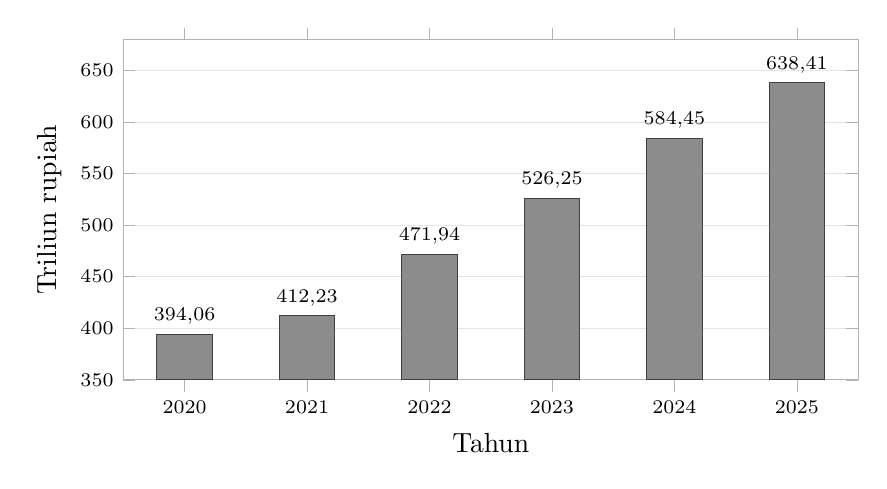
\begin{tikzpicture}
        \begin{axis}[
                width=0.9\textwidth,
                height=5.9cm,
                ybar,
                bar width=20pt,
                ymin=350, ymax=680,
                ylabel={Triliun rupiah},
                xlabel={Tahun},
                symbolic x coords={2020,2021,2022,2023,2024,2025},
                xtick=data,
                ymajorgrids=true,
                grid style={gray!20},
                axis line style={gray!60},
                tick style={gray!60},
                ytick={350,400,450,500,550,600,650},
                yticklabel style={font=\scriptsize},
                x tick label style={font=\scriptsize},
                enlarge x limits=0.10,
                clip=false
            ]
            \addplot[
                fill=black!45,
                draw=black!75
            ] coordinates {
                    (2020,394.06) (2021,412.23) (2022,471.94) (2023,526.25) (2024,584.45) (2025,638.41)
                };
            \node[font=\scriptsize, anchor=south] at (axis cs:2020,394.06) {394,06};
            \node[font=\scriptsize, anchor=south] at (axis cs:2021,412.23) {412,23};
            \node[font=\scriptsize, anchor=south] at (axis cs:2022,471.94) {471,94};
            \node[font=\scriptsize, anchor=south] at (axis cs:2023,526.25) {526,25};
            \node[font=\scriptsize, anchor=south] at (axis cs:2024,584.45) {584,45};
            \node[font=\scriptsize, anchor=south] at (axis cs:2025,638.41) {638,41};
        \end{axis}
    \end{tikzpicture}
    \figuresource[0.9\textwidth]{Diolah peneliti dari BPS \parencite{bps2025pendapatan,bps2026ekonomiindonesia}.}
    \caption{Tren PDB lapangan usaha penyediaan akomodasi dan makan minum di Indonesia atas dasar harga berlaku}
    \label{fig:tren-pdb-makan-minum-indonesia}
\end{figure}

\begin{figure}[!t]
    \centering
    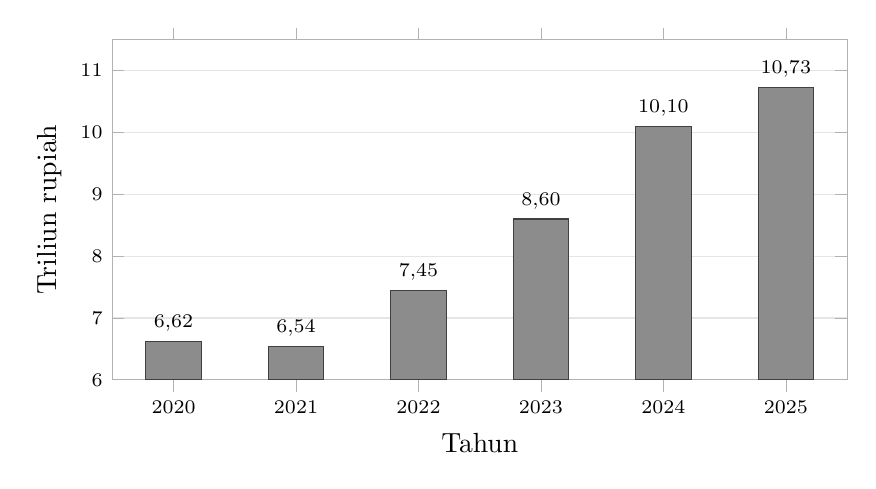
\begin{tikzpicture}
        \begin{axis}[
                width=0.9\textwidth,
                height=5.9cm,
                ybar,
                bar width=20pt,
                ymin=6, ymax=11.5,
                ylabel={Triliun rupiah},
                xlabel={Tahun},
                symbolic x coords={2020,2021,2022,2023,2024,2025},
                xtick=data,
                ymajorgrids=true,
                grid style={gray!20},
                axis line style={gray!60},
                tick style={gray!60},
                ytick={6,7,8,9,10,11},
                yticklabel style={font=\scriptsize},
                x tick label style={font=\scriptsize},
                enlarge x limits=0.10,
                clip=false
            ]
            \addplot[
                fill=black!45,
                draw=black!75
            ] coordinates {
                    (2020,6.62) (2021,6.54) (2022,7.45) (2023,8.60) (2024,10.10) (2025,10.73)
                };
            \node[font=\scriptsize, anchor=south] at (axis cs:2020,6.62) {6,62};
            \node[font=\scriptsize, anchor=south] at (axis cs:2021,6.54) {6,54};
            \node[font=\scriptsize, anchor=south] at (axis cs:2022,7.45) {7,45};
            \node[font=\scriptsize, anchor=south] at (axis cs:2023,8.60) {8,60};
            \node[font=\scriptsize, anchor=south] at (axis cs:2024,10.10) {10,10};
            \node[font=\scriptsize, anchor=south] at (axis cs:2025,10.73) {10,73};
        \end{axis}
    \end{tikzpicture}
    \figuresource[0.9\textwidth]{Diolah peneliti dari BPS Kota Medan \parencite{bpsmedan2025pdrb,bpsmedan2026pdrb}.}
    \caption{Tren PDRB lapangan usaha penyediaan akomodasi dan makan minum di Kota Medan atas dasar harga berlaku}
    \label{fig:tren-pdrb-makan-minum-medan}
\end{figure}

Pertumbuhan jumlah usaha kuliner menyebabkan tingkat persaingan semakin ketat. Pelaku usaha tidak hanya bersaing dari sisi rasa, tetapi juga dari variasi menu, harga, kemasan, lokasi, kecepatan layanan, promosi, reputasi, dan kemudahan akses pembelian. Dalam kondisi pasar yang padat, usaha kuliner membutuhkan strategi pemasaran yang efektif agar mampu menarik pelanggan baru, mempertahankan pelanggan lama, dan menjaga daya saing terhadap kompetitor. Pemasaran dalam konteks ini dipahami sebagai proses menciptakan, mengomunikasikan, menyampaikan, dan mempertukarkan nilai kepada konsumen \parencite{kotler2021marketingmanagement}. Oleh karena itu, strategi pemasaran perlu disusun berdasarkan pemahaman terhadap kebutuhan pasar, karakter konsumen, kekuatan usaha, serta tekanan persaingan yang dihadapi.

Pemasaran usaha kuliner dapat dilakukan melalui saluran offline dan online. Pemasaran offline umumnya dilakukan melalui lokasi fisik, papan nama, rekomendasi dari mulut ke mulut, pelayanan langsung, kerja sama komunitas, dan promosi di sekitar area usaha. Sementara itu, pemasaran online dilakukan melalui media sosial, katalog digital, mesin pencari, aplikasi pesan, marketplace, serta platform pesan antar makanan. Perkembangan pemasaran digital menjadi penting karena konsumen kini dapat menemukan, membandingkan, memesan, dan menilai produk kuliner melalui perangkat digital \parencite{chaffey2022digitalmarketing,regina2025kuliner}. Bagi UMKM kuliner, penggunaan kanal digital dapat memperluas jangkauan pasar, meningkatkan visibilitas, dan mempercepat transaksi ketika dikelola secara konsisten \parencite{regina2025kuliner,mamuriyah2021gadihminang,roslam2021markisaaurora,suharjo2020bogorsnacks}.

Salah satu bentuk pemasaran online yang banyak digunakan pelaku usaha kuliner adalah platform marketplace atau \textit{online food delivery} seperti ShopeeFood, GoFood, dan GrabFood. Platform tersebut tidak hanya berfungsi sebagai media pemesanan, tetapi juga menjadi etalase digital yang menampilkan nama usaha, foto menu, harga, promo, rating, ulasan pelanggan, dan estimasi layanan. Kajian terdahulu menunjukkan bahwa pemanfaatan platform digital dapat membantu UMKM memperluas jangkauan pasar dan meningkatkan penjualan ketika fitur platform, promosi, tampilan produk, serta komunikasi dengan pelanggan dikelola secara konsisten \parencite{regina2025kuliner,sophia2025rendanggadih,suharjo2020bogorsnacks}. Hal ini menunjukkan bahwa platform seperti GrabFood telah menjadi ruang pemasaran dan persaingan yang penting bagi usaha kuliner.

Rumah Makan Nasi Gerilya merupakan usaha nasi Padang di Kota Medan yang memanfaatkan kanal online dalam aktivitas penjualannya. Berdasarkan wawancara awal dengan pemilik, Nasi Gerilya menggunakan GrabFood, GoFood, dan ShopeeFood sebagai kanal penjualan online, tetapi GrabFood menjadi platform utama karena dinilai paling sesuai dengan target pasar usaha. Pemilik juga menyampaikan bahwa GrabFood berkontribusi lebih dari 50\% terhadap \textit{revenue} usaha, sehingga platform ini tidak hanya berperan sebagai saluran tambahan, tetapi sebagai salah satu kanal penjualan utama. Hasil observasi toko pada GrabFood menunjukkan bahwa Nasi Gerilya memiliki rating 4,7/5,0, 4.187 ulasan, rentang harga Rp11.000--Rp72.000, promo platform aktif, serta menu teratas seperti rendang sapi, ayam goreng, ayam bakar, dan nasi bakar kikil tunjang. Keempat menu teratas tersebut menunjukkan variasi harga utama yang ditawarkan Nasi Gerilya pada GrabFood sebagaimana disajikan pada Tabel~\ref{tab:harga-menu-teratas-gerilya}.

\begin{table}[!t]
    \centering
    \caption{Harga Menu Teratas Rumah Makan Nasi Gerilya pada GrabFood}
    \label{tab:harga-menu-teratas-gerilya}
    \small
    \renewcommand{\arraystretch}{1.08}
    \begin{tabularx}{0.82\textwidth}{|X|>{\raggedleft\arraybackslash}p{3cm}|}
        \toprule
        \textbf{Menu Teratas}    & \textbf{Harga} \\ \hline
        \midrule
        Nasi Padang Rendang Sapi & Rp56.000       \\ \hline
        Nasi Padang Ayam Goreng  & Rp45.000       \\ \hline
        Nasi Padang Ayam Bakar   & Rp45.000       \\ \hline
        Nasi Bakar Kikil Tunjang & Rp68.000       \\ \hline
        \bottomrule
    \end{tabularx}
    \tablesource[0.82\textwidth]{Observasi platform GrabFood pada 04 April 2026; diolah peneliti (2026).}
\end{table}

Menu selebihnya disajikan secara lebih lengkap pada Lampiran Tabel~\ref{tab:survei_harga_nasi_gerilya_grabfood}. Data awal mengenai observasi GrabFood, wawancara awal pemilik, dan dokumentasi kinerja usaha disajikan lebih lengkap pada Lampiran~\ref{app:observasi-grabfood}, Lampiran~\ref{app:wawancara-awal-pemilik}, dan Lampiran~\ref{app:dokumentasi-indeks-kinerja}. Visual pendukung pada Gambar~\ref{fig:tren-penjualan-bungkus-gerilya} menunjukkan bahwa jumlah penjualan Nasi Gerilya meningkat dari 6.702 bungkus pada Desember 2024 menjadi 16.590 bungkus pada Maret 2025, tetapi kemudian menurun bertahap menjadi 12.900 bungkus pada November 2025. Gambar~\ref{fig:komposisi-pelanggan-gerilya} juga menunjukkan bahwa pelanggan baru meningkat dari 45\% menjadi 55\%, sedangkan \textit{repeat order} menurun dari 43\% menjadi 38\%. Kondisi tersebut menunjukkan bahwa eksposur digital dan kontribusi GrabFood yang besar belum otomatis menjamin stabilitas penjualan dan loyalitas pelanggan.

\begin{figure}[!t]
    \centering
    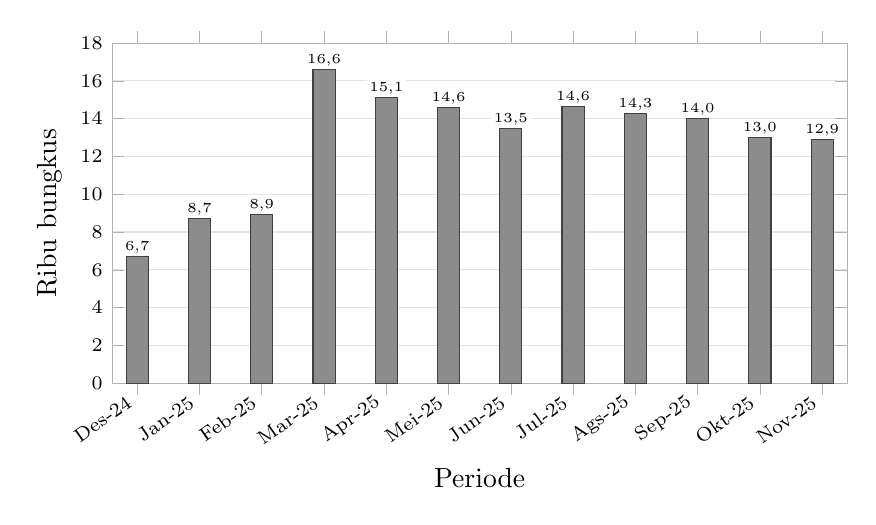
\begin{tikzpicture}
        \begin{axis}[
                width=0.9\textwidth,
                height=5.9cm,
                ybar,
                bar width=8pt,
                xmin=-0.4, xmax=11.4,
                ymin=0, ymax=18,
                ylabel={Ribu bungkus},
                xlabel={Periode},
                ymajorgrids=true,
                grid style={gray!20},
                axis line style={gray!60},
                tick style={gray!60},
                xtick=data,
                xticklabels={Des-24,Jan-25,Feb-25,Mar-25,Apr-25,Mei-25,Jun-25,Jul-25,Ags-25,Sep-25,Okt-25,Nov-25},
                x tick label style={rotate=35, anchor=east, font=\scriptsize},
                ytick={0,2,4,6,8,10,12,14,16,18},
                yticklabel style={font=\scriptsize},
                clip=false
            ]
            \addplot[
                fill=black!45,
                draw=black!75
            ] coordinates {
                    (0,6.702) (1,8.740) (2,8.911) (3,16.590) (4,15.129) (5,14.580)
                    (6,13.467) (7,14.633) (8,14.259) (9,14.034) (10,13.009) (11,12.900)
                };
            \node[font=\tiny, fill=white, inner sep=1pt, anchor=south] at (axis cs:0,6.702) {6,7};
            \node[font=\tiny, fill=white, inner sep=1pt, anchor=south] at (axis cs:1,8.740) {8,7};
            \node[font=\tiny, fill=white, inner sep=1pt, anchor=south] at (axis cs:2,8.911) {8,9};
            \node[font=\tiny, fill=white, inner sep=1pt, anchor=south] at (axis cs:3,16.590) {16,6};
            \node[font=\tiny, fill=white, inner sep=1pt, anchor=south] at (axis cs:4,15.129) {15,1};
            \node[font=\tiny, fill=white, inner sep=1pt, anchor=south] at (axis cs:5,14.580) {14,6};
            \node[font=\tiny, fill=white, inner sep=1pt, anchor=south] at (axis cs:6,13.467) {13,5};
            \node[font=\tiny, fill=white, inner sep=1pt, anchor=south] at (axis cs:7,14.633) {14,6};
            \node[font=\tiny, fill=white, inner sep=1pt, anchor=south] at (axis cs:8,14.259) {14,3};
            \node[font=\tiny, fill=white, inner sep=1pt, anchor=south] at (axis cs:9,14.034) {14,0};
            \node[font=\tiny, fill=white, inner sep=1pt, anchor=south] at (axis cs:10,13.009) {13,0};
            \node[font=\tiny, fill=white, inner sep=1pt, anchor=south] at (axis cs:11,12.900) {12,9};
        \end{axis}
    \end{tikzpicture}
    \figuresource[0.9\textwidth]{Diolah peneliti dari dokumentasi grafik penjualan bulanan Nasi Gerilya.}
    \caption{Tren jumlah penjualan bulanan Nasi Gerilya dalam satuan bungkus}
    \label{fig:tren-penjualan-bungkus-gerilya}
\end{figure}

\begin{figure}[!t]
    \centering
    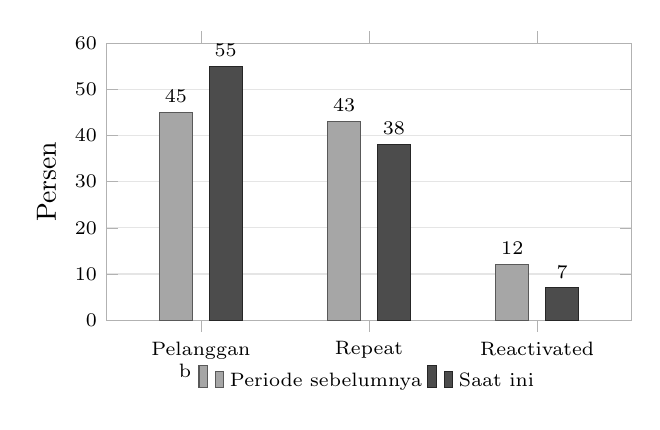
\begin{tikzpicture}
        \begin{axis}[
                width=0.68\textwidth,
                height=5.1cm,
                ybar=6pt,
                bar width=12pt,
                ymin=0, ymax=60,
                ylabel={Persen},
                ymajorgrids=true,
                grid style={gray!20},
                axis line style={gray!60},
                tick style={gray!60},
                symbolic x coords={Baru,Repeat,Reactivated},
                xtick=data,
                xticklabels={Pelanggan\\baru,Repeat\\order,Reactivated},
                x tick label style={font=\scriptsize, align=center},
                ytick={0,10,20,30,40,50,60},
                yticklabel style={font=\scriptsize},
                nodes near coords,
                every node near coord/.append style={font=\scriptsize},
                enlarge x limits=0.28,
                legend style={
                        font=\scriptsize,
                        draw=none,
                        at={(0.5,-0.14)},
                        anchor=north,
                        legend columns=2
                    }
            ]
            \addplot[fill=black!35, draw=black!65] coordinates {(Baru,45) (Repeat,43) (Reactivated,12)};
            \addplot[fill=black!70, draw=black!85] coordinates {(Baru,55) (Repeat,38) (Reactivated,7)};
            \legend{Periode sebelumnya,Saat ini}
        \end{axis}
    \end{tikzpicture}
    \figuresource[0.68\textwidth]{Diolah peneliti dari wawancara awal dengan pemilik usaha.}
    \caption{Perubahan komposisi pelanggan Nasi Gerilya berdasarkan wawancara awal pemilik usaha}
    \label{fig:komposisi-pelanggan-gerilya}
\end{figure}
Dalam kondisi tersebut, bauran pemasaran atau \textit{marketing mix} menjadi konsep yang relevan untuk membaca strategi pemasaran Nasi Gerilya. Konsep 4P menempatkan \textit{product}, \textit{price}, \textit{place}, dan \textit{promotion} sebagai perangkat utama dalam mengelola penawaran pasar \parencite{kotler2023principlesmarketing}. Pada bisnis jasa dan kuliner, bauran tersebut dapat diperluas menjadi 7P dengan menambahkan \textit{people}, \textit{process}, dan \textit{physical evidence} karena pengalaman pelanggan juga dipengaruhi oleh pelaksana layanan, proses pemenuhan pesanan, serta bukti kualitas yang terlihat oleh konsumen \parencite{wirtz2024servicesmarketing}. Dalam konteks Nasi Gerilya pada GrabFood, unsur produk terlihat dari variasi menu dan konsistensi rasa; harga terlihat dari rentang harga, ongkos kirim, dan promo; tempat terlihat dari penggunaan GrabFood sebagai kanal distribusi online; promosi terlihat dari voucher, promo platform, media sosial, dan KOL; \textit{people} terlihat dari kesiapan admin, karyawan, dan juru masak; \textit{process} terlihat dari kecepatan layanan, pengelolaan menu habis, dan ketepatan pesanan; sedangkan \textit{physical evidence} terlihat dari foto produk, kemasan, rating, dan ulasan pelanggan.

Review pelanggan menjadi bagian penting dalam evaluasi strategi pemasaran karena platform \textit{online food delivery} membuat pengalaman pelanggan terekam secara terbuka melalui rating, komentar, keluhan, dan rekomendasi. Penelitian terdahulu menunjukkan bahwa harga, promosi, tampilan produk, kualitas layanan, ulasan, dan peringkat pada platform digital dapat memengaruhi keputusan pembelian serta performa penjualan usaha kuliner \parencite{sophia2025rendanggadih,ruhiyat2023minatbeli,khairani2022buahsayur,suharjo2020bogorsnacks}. Pada Nasi Gerilya, review pelanggan memuat komentar positif mengenai rasa enak, bumbu dan rempah yang kuat, porsi besar, bahan segar, kemasan rapi, variasi menu, serta harga yang dinilai terjangkau. Namun, review tersebut juga memuat keluhan mengenai rasa yang dianggap berubah, pesanan tidak lengkap, menu tidak tersedia, lauk utama yang dinilai kurang besar atau kurang segar, nasi yang kadang keras, proporsi nasi dan lauk yang kurang seimbang, serta suhu makanan yang tidak selalu konsisten. Oleh karena itu, review pelanggan, komentar, keluhan, dan permasalahan layanan menjadi dasar penting untuk mengevaluasi serta meningkatkan strategi pemasaran Nasi Gerilya pada GrabFood.

\section{Rumusan Masalah}
Berdasarkan latar belakang di atas, maka rumusan masalah dalam penelitian ini adalah:
\begin{enumerate}
    \item Bagaimana faktor internal Rumah Makan Nasi Gerilya pada platform GrabFood yang mencakup kekuatan dan kelemahan usaha?
    \item Bagaimana faktor eksternal Rumah Makan Nasi Gerilya pada platform GrabFood yang mencakup peluang dan ancaman usaha?
    \item Bagaimana strategi pemasaran Rumah Makan Nasi Gerilya pada platform GrabFood berdasarkan analisis matriks SWOT?
\end{enumerate}

\section{Tujuan Penelitian}
Tujuan yang ingin dicapai dalam penelitian ini adalah sebagai berikut:
\begin{enumerate}
    \item Untuk mengidentifikasi faktor internal Rumah Makan Nasi Gerilya pada platform GrabFood yang mencakup kekuatan dan kelemahan usaha.
    \item Untuk mengidentifikasi faktor eksternal Rumah Makan Nasi Gerilya pada platform GrabFood yang mencakup peluang dan ancaman usaha.
    \item Untuk merumuskan strategi pemasaran Rumah Makan Nasi Gerilya pada platform GrabFood berdasarkan analisis matriks SWOT.
\end{enumerate}

\section{Manfaat Penelitian}
Penelitian ini diharapkan dapat bermanfaat secara teoretis dan praktis:
\subsection{Manfaat Teoretis}
Penelitian ini diharapkan dapat berkontribusi dalam pengembangan ilmu manajemen pemasaran, khususnya yang berkaitan dengan strategi pemasaran usaha kuliner pada platform \textit{online food delivery}, terutama GrabFood. Selain itu, penelitian ini juga diharapkan dapat memperkaya kajian mengenai penerapan analisis SWOT dalam mengidentifikasi faktor internal dan faktor eksternal usaha sebagai dasar perumusan strategi pemasaran. Hasil penelitian ini selanjutnya diharapkan dapat menjadi bahan referensi bagi peneliti lain yang ingin mengkaji topik serupa, terutama pada konteks UMKM kuliner yang memanfaatkan platform digital sebagai saluran pemasaran.
\subsection{Manfaat Praktis}
Secara praktis, penelitian ini diharapkan dapat memberikan manfaat bagi beberapa pihak sebagai berikut:
\subsubsection{Bagi Rumah Makan Nasi Gerilya}
\noindent Penelitian ini diharapkan dapat menjadi bahan masukan dan evaluasi dalam mengidentifikasi kekuatan, kelemahan, peluang, dan ancaman usaha pada platform GrabFood. Dengan demikian, hasil penelitian ini dapat digunakan sebagai dasar dalam merumuskan strategi pemasaran yang lebih tepat untuk mempertahankan daya saing dan meningkatkan kinerja usaha.
\subsubsection{Bagi Pelaku Usaha Kuliner}
\noindent Penelitian ini diharapkan dapat menjadi gambaran dan bahan pertimbangan bagi pelaku usaha kuliner lainnya mengenai pentingnya analisis kondisi internal dan eksternal usaha dalam menyusun strategi pemasaran pada platform \textit{online food delivery}.
\subsubsection{Bagi Akademisi}
\noindent Penelitian ini diharapkan dapat menjadi tambahan acuan dan referensi ilmiah, khususnya yang berkaitan dengan strategi pemasaran kuliner berbasis platform, strategi pemasaran UMKM, dan penerapan analisis SWOT pada sektor kuliner.

\chapter{TINJAUAN PUSTAKA}

\section{Landasan Teoritis}
\subsection{Pemasaran}
Pemasaran merupakan konsep dasar yang perlu dijelaskan terlebih dahulu karena penelitian ini membahas cara Rumah Makan Nasi Gerilya menyusun penawaran dan menjangkau konsumen melalui GrabFood. Pemasaran tidak hanya berarti kegiatan menjual atau mempromosikan produk, tetapi mencakup proses menciptakan, mengomunikasikan, menyampaikan, dan mempertukarkan nilai kepada pelanggan secara menguntungkan \parencite{kotler2021marketingmanagement,kotler2023principlesmarketing}. Dalam pandangan pemasaran modern, nilai pelanggan terbentuk ketika kebutuhan konsumen, kemampuan usaha, dan penawaran pasar bertemu dalam bentuk produk, harga, akses pembelian, komunikasi, serta pengalaman layanan yang dianggap relevan oleh konsumen \parencite{kotler2023principlesmarketing,wirtz2024servicesmarketing}. Karena itu, pemasaran menjadi landasan untuk memahami mengapa sebuah usaha kuliner tidak cukup hanya memiliki produk yang baik, tetapi juga perlu mengelola cara produk tersebut dipersepsikan, ditemukan, dipilih, dibeli, dan dinilai oleh konsumen.

Pada usaha kuliner, pemasaran berperan sebagai penghubung antara kemampuan internal usaha dengan kebutuhan pasar yang terus berubah. Konsumen makanan tidak hanya menilai cita rasa, tetapi juga variasi menu, keterjangkauan harga, kemudahan akses, kecepatan layanan, tampilan produk, reputasi, serta konsistensi pengalaman pembelian \parencite{regina2025kuliner,sophia2025rendanggadih,wirtz2024servicesmarketing}. Ketika pembelian dilakukan melalui platform digital, ruang pemasaran semakin meluas karena konsumen mengambil keputusan berdasarkan informasi yang tersaji di aplikasi, seperti nama menu, foto produk, deskripsi, harga, promo, rating, dan ulasan \parencite{hidayah2021digitalplatforms,putri2024cikarang,elverda2025ofdindonesia}. Dengan demikian, pemasaran dalam penelitian ini menjadi pijakan awal untuk membaca aktivitas Nasi Gerilya sebagai upaya menyusun nilai produk dan pengalaman pembelian yang sesuai dengan karakter pasar digital.

\subsection{Strategi Pemasaran}
Strategi pemasaran merupakan kelanjutan dari konsep pemasaran karena strategi menjelaskan arah dan cara usaha mengelola nilai yang ditawarkan kepada pasar sasaran. Dalam pemasaran modern, strategi tidak hanya dipahami sebagai kegiatan promosi, tetapi sebagai keputusan terpadu mengenai siapa yang dilayani, nilai apa yang ditawarkan, dan bagaimana nilai tersebut disampaikan secara lebih unggul daripada pesaing \parencite{kotler2021marketingmanagement,kotler2023principlesmarketing}. Pemahaman ini sejalan dengan pandangan manajemen strategis yang menempatkan strategi sebagai proses penyesuaian antara tujuan organisasi, kemampuan internal, dan tekanan lingkungan eksternal \parencite{david2023strategicmanagement}. Dengan demikian, strategi pemasaran perlu dibaca sebagai jembatan antara tujuan usaha dan kondisi pasar yang dihadapi, bukan sebagai kegiatan yang berdiri sendiri.

Pada usaha kuliner, strategi pemasaran semakin penting karena persaingan tidak hanya berlangsung pada kualitas rasa, tetapi juga pada variasi menu, harga, kemasan, promosi, akses pemesanan, dan pengalaman layanan yang melekat pada proses pembelian \parencite{regina2025kuliner,sophia2025rendanggadih}. Perubahan menuju pemasaran digital membuat keputusan strategis menjadi lebih kompleks karena usaha perlu mengelola tampilan produk, informasi menu, promosi, dan kanal transaksi secara bersamaan \parencite{chaffey2022digitalmarketing,hidayah2021digitalplatforms}. Dalam konteks UMKM kuliner, penelitian sebelumnya menunjukkan bahwa penguatan strategi digital dapat membantu meningkatkan visibilitas, memperluas jangkauan pasar, dan memperbaiki kinerja usaha ketika didukung oleh kesiapan organisasi serta pemilihan kanal yang tepat \parencite{putro2025digitaltransformation,regina2025kuliner}. Oleh karena itu, strategi pemasaran pada Rumah Makan Nasi Gerilya perlu dipahami sebagai rangkaian keputusan yang menghubungkan kekuatan produk, pengelolaan platform GrabFood, dan respons terhadap persaingan pasar.

Strategi tersebut harus mampu menerjemahkan pemahaman tentang konsumen menjadi keputusan yang lebih operasional, mulai dari penentuan pasar sasaran, posisi usaha, susunan menu, harga, promosi, saluran pemasaran, hingga cara usaha merespons peluang dan ancaman di dalam platform \parencite{kotler2023principlesmarketing,chaffey2022digitalmarketing,david2023strategicmanagement}. Karena fokus penelitian ini adalah perumusan strategi, konsep strategi pemasaran menjadi dasar untuk menempatkan STP, bauran pemasaran, pemasaran digital, saluran OFDA, analisis lingkungan, dan SWOT sebagai bagian yang saling melengkapi.

\subsection{STP dan Bauran Pemasaran}
Segmentasi, \textit{targeting}, dan \textit{positioning} (STP) melengkapi strategi pemasaran karena membantu usaha menentukan kelompok pasar yang ingin dilayani dan citra yang ingin dibangun di benak konsumen \parencite{kotler2021marketingmanagement,kotler2023principlesmarketing}. Segmentasi diperlukan karena pasar kuliner tidak homogen; konsumen dapat berbeda dalam daya beli, waktu pembelian, preferensi menu, sensitivitas harga, dan respons terhadap promosi \parencite{suharjo2020bogorsnacks,ruhiyat2023minatbeli}. Setelah segmen dipahami, usaha perlu memilih segmen yang paling sesuai dengan kapasitas dan tujuan usahanya, lalu membangun \textit{positioning} yang membedakan penawarannya dari pesaing \parencite{kotler2023principlesmarketing,sophia2025rendanggadih}. Pada konteks Nasi Gerilya, STP menjadi penting karena strategi pemasaran di GrabFood perlu menjelaskan pasar sasaran, posisi harga, identitas rasa, dan alasan konsumen memilih usaha tersebut dibanding \textit{merchant} sejenis.

Bauran pemasaran menerjemahkan STP menjadi tindakan pemasaran yang lebih operasional. Konsep 4P menempatkan \textit{product}, \textit{price}, \textit{place}, dan \textit{promotion} sebagai perangkat utama untuk mengelola penawaran pasar \parencite{kotler2021marketingmanagement,kotler2023principlesmarketing}. Dalam usaha kuliner digital, produk tidak hanya berupa makanan, tetapi juga variasi menu, kemasan, foto, dan kejelasan deskripsi; harga tidak hanya berupa nominal menu, tetapi juga potongan harga, ongkos kirim, dan paket promosi; tempat tidak hanya berarti lokasi fisik, tetapi juga kanal distribusi digital; sedangkan promosi mencakup voucher, kampanye platform, dan komunikasi visual \parencite{chaffey2022digitalmarketing,hidayah2021digitalplatforms,putri2024cikarang}. Penelitian tentang strategi pemasaran kuliner berbasis platform juga menunjukkan bahwa penerapan STP dan bauran pemasaran dapat membantu usaha mengarahkan penjualan ketika fitur platform dimanfaatkan secara konsisten \parencite{sophia2025rendanggadih,firdaus2022bangkupawon}.

Pada bisnis jasa dan kuliner, bauran pemasaran sering diperluas menjadi 7P dengan menambahkan \textit{people}, \textit{process}, dan \textit{physical evidence}, karena keberhasilan pemasaran tidak hanya ditentukan oleh penawaran inti, tetapi juga oleh pelaksana layanan, proses pemenuhan pesanan, dan bukti yang memperkuat persepsi kualitas \parencite{wirtz2024servicesmarketing}. Dalam konteks OFDA, unsur tersebut terlihat dari kesiapan admin dan karyawan, kecepatan konfirmasi, akurasi pesanan, pengelolaan menu habis, tampilan etalase digital, foto produk, kemasan, rating, dan ulasan \parencite{hidayah2021digitalplatforms,putri2024cikarang,elverda2025ofdindonesia}. Dengan demikian, STP dan bauran pemasaran saling melengkapi: STP membantu menentukan arah pasar dan posisi usaha, sedangkan bauran pemasaran membantu menilai apakah keputusan produk, harga, distribusi, promosi, proses, pelaksana layanan, dan bukti digital sudah mendukung posisi tersebut.

\subsection{Pemasaran Digital}
Pemasaran digital memperluas pembahasan strategi pemasaran karena teknologi digital mengubah cara usaha menciptakan, mengomunikasikan, dan menyampaikan nilai kepada pasar \parencite{chaffey2022digitalmarketing}. Berbeda dari pemasaran konvensional yang sering bergantung pada komunikasi satu arah, pemasaran digital memungkinkan interaksi, pengukuran respons, dan penyesuaian pesan secara lebih cepat melalui data kunjungan, klik, ulasan, transaksi, dan keterlibatan konsumen \parencite{chaffey2022digitalmarketing,purnomo2023conversion}. Dalam konteks usaha kuliner, pemasaran digital tidak hanya berarti mengunggah konten promosi, tetapi juga mengelola katalog menu, foto produk, deskripsi, promosi, kanal pemesanan, dan reputasi digital \parencite{regina2025kuliner,hidayah2021digitalplatforms}. Dengan demikian, pemasaran digital menjadi bagian dari strategi bisnis yang menghubungkan aktivitas promosi, distribusi, transaksi, dan evaluasi pasar.

Pemasaran digital relevan bagi UMKM kuliner karena usaha kecil sering menghadapi keterbatasan lokasi, modal promosi, dan jangkauan pelanggan, sedangkan platform digital membuka peluang untuk memperluas pasar dengan biaya yang relatif lebih fleksibel \parencite{fatmawatie2022turnover,regina2025kuliner}. Penelitian \textcite{putro2025digitaltransformation} menunjukkan bahwa transformasi digital berpengaruh terhadap kinerja UMKM kuliner melalui dukungan teknologi, organisasi, dan lingkungan. Kajian lain menunjukkan bahwa penggunaan media sosial, katalog daring, \textit{e-commerce}, dan aplikasi pesan antar dapat meningkatkan visibilitas, penjualan, dan keterhubungan usaha dengan konsumen ketika dikelola secara konsisten \parencite{hidayah2021digitalplatforms,indriyani2025gudangbaju,pratama2024sambelmoji}. Oleh karena itu, pemasaran digital dalam penelitian ini diposisikan sebagai konteks strategis yang membantu membaca bagaimana Nasi Gerilya memanfaatkan GrabFood sebagai kanal pemasaran, bukan sekadar sebagai aplikasi pemesanan.

\subsection{Saluran Pemasaran (OFDA)}
\textit{Online food delivery application} (OFDA) merupakan saluran digital yang mempertemukan usaha makanan dengan konsumen melalui sistem yang mengintegrasikan informasi produk, pemesanan, pembayaran, promosi, dan pengantaran \parencite{zaheer2024ofda,elverda2025ofdindonesia}. Dalam kajian strategi pemasaran, OFDA tidak hanya dipahami sebagai alat distribusi, tetapi juga sebagai etalase digital, ruang promosi, sumber reputasi, dan arena persaingan antar \textit{merchant} \parencite{chaffey2022digitalmarketing,putri2024cikarang}. Karakteristik ini membuat keputusan strategi pada platform seperti GrabFood perlu memperhatikan keterpaduan antara menu, harga, foto, deskripsi, promo, ketersediaan toko, rating, dan posisi terhadap pesaing \parencite{hidayah2021digitalplatforms,firdaus2022bangkupawon}.

Peran OFDA dalam usaha kuliner berkaitan langsung dengan bauran pemasaran karena produk ditampilkan melalui nama menu dan visual, harga ditampilkan bersama potongan dan ongkos kirim, distribusi dilakukan melalui jaringan pengantaran, sedangkan promosi dijalankan melalui voucher, kampanye platform, dan paket bundling \parencite{putri2024cikarang,sophia2025rendanggadih}. Penelitian tentang pemanfaatan GrabFood dan GoFood menunjukkan bahwa platform pesan antar dapat membantu UMKM memperluas jangkauan pasar dan meningkatkan penjualan, tetapi manfaat tersebut tetap bergantung pada kemampuan usaha mengelola fitur platform secara tepat \parencite{firdaus2022bangkupawon,putri2024cikarang}. Dengan demikian, OFDA dalam penelitian ini menjadi konteks strategis untuk membaca bagaimana Nasi Gerilya mengelola saluran GrabFood dan bagaimana dinamika platform tersebut memunculkan peluang maupun ancaman bagi strategi pemasaran.

\subsection{Analisis Lingkungan}
Analisis lingkungan diperlukan karena strategi pemasaran harus disusun berdasarkan kondisi nyata usaha dan dinamika pasar yang dihadapi. Dalam manajemen strategis, lingkungan internal menggambarkan sumber daya dan kemampuan yang berada dalam kendali usaha, sedangkan lingkungan eksternal menggambarkan kondisi pasar, pesaing, teknologi, kebijakan, dan perubahan perilaku konsumen yang memengaruhi ruang gerak usaha \parencite{david2023strategicmanagement,kotler2023principlesmarketing}. Dalam kerangka SWOT, faktor internal menjadi dasar untuk menentukan kekuatan dan kelemahan, sedangkan faktor eksternal menjadi dasar untuk menentukan peluang dan ancaman \parencite{gurel2017swot,helms2010swotreview}. Dengan demikian, analisis lingkungan membantu penelitian ini menghindari perumusan strategi yang hanya bertumpu pada keinginan usaha, karena strategi perlu disesuaikan dengan kapasitas internal dan tekanan eksternal.

\subsubsection{Lingkungan Internal}
Lingkungan internal pada usaha kuliner dapat dilihat melalui beberapa bidang, seperti sumber daya manusia, keuangan, produksi, operasional, pemasaran, dan teknologi. Aspek sumber daya manusia berkaitan dengan jumlah karyawan, pembagian tugas, kemampuan mengelola pesanan, kecepatan pelayanan, dan kedisiplinan dalam menjaga standar kerja \parencite{wirtz2024servicesmarketing,david2023strategicmanagement}. Aspek keuangan berkaitan dengan kemampuan usaha mengatur harga, biaya bahan baku, biaya promosi, potongan platform, dan margin penjualan agar strategi promosi tidak menurunkan keberlanjutan usaha \parencite{kotler2023principlesmarketing,david2023strategicmanagement}. Aspek produksi dan operasional mencakup konsistensi rasa, kualitas bahan, variasi menu, ketersediaan stok, pengemasan, akurasi pesanan, dan ketepatan waktu pemrosesan pesanan \parencite{regina2025kuliner,sophia2025rendanggadih,putri2024cikarang}. Aspek pemasaran dan teknologi mencakup kemampuan usaha memperbarui menu, mengelola foto dan deskripsi produk, menjalankan promo, membaca ulasan, serta memanfaatkan fitur GrabFood sebagai kanal pemasaran \parencite{chaffey2022digitalmarketing,hidayah2021digitalplatforms,firdaus2022bangkupawon}. Keseluruhan aspek tersebut menentukan apakah kekuatan Nasi Gerilya dapat dimaksimalkan dan apakah kelemahannya perlu diperbaiki sebelum strategi baru dijalankan.

\subsubsection{Lingkungan Eksternal}
Lingkungan eksternal melengkapi analisis internal karena usaha kuliner berbasis platform tidak beroperasi dalam ruang yang sepenuhnya dapat dikendalikan. Faktor eksternal dapat mencakup pertumbuhan penggunaan platform pesan antar, kebiasaan konsumen mencari makanan secara daring, kebijakan biaya layanan, program promo platform, ongkos kirim, algoritma visibilitas toko, rating, ulasan, serta kehadiran \textit{merchant} pesaing dengan produk dan harga yang sebanding \parencite{hidayah2021digitalplatforms,putri2024cikarang,elverda2025ofdindonesia}. Penelitian tentang strategi digital UMKM menunjukkan bahwa media digital dan platform dapat membuka peluang peningkatan penjualan, tetapi peluang tersebut dapat melemah ketika usaha menghadapi tekanan pesaing, perang promo, keterbatasan modal promosi, atau ketidakmampuan mengelola kanal digital secara konsisten \parencite{saptaji2025karawang,azzahra2024guzzini,indriyani2025gudangbaju}. Oleh karena itu, analisis lingkungan pada Nasi Gerilya digunakan untuk membaca hubungan antara kapasitas internal seperti SDM, keuangan, operasional, dan pemasaran dengan kondisi eksternal seperti kebijakan GrabFood, perilaku konsumen, persaingan kategori, serta perubahan saluran pemasaran digital.

\subsection{SWOT}
Analisis SWOT menjadi alat utama dalam penelitian ini karena SWOT menghubungkan faktor internal dan faktor eksternal ke dalam empat kategori strategis, yaitu \textit{strengths}, \textit{weaknesses}, \textit{opportunities}, dan \textit{threats} \parencite{helms2010swotreview,gurel2017swot}. Kekuatan dan kelemahan berasal dari kondisi internal usaha, sedangkan peluang dan ancaman berasal dari lingkungan eksternal yang memengaruhi arah keputusan strategis \parencite{david2023strategicmanagement,gurel2017swot}. Keunggulan SWOT terletak pada kemampuannya menyusun informasi yang tersebar menjadi peta strategis yang mudah dibaca, tetapi kajian terdahulu juga menekankan bahwa SWOT perlu digunakan secara sistematis agar tidak berhenti sebagai daftar faktor semata \parencite{helms2010swotreview,david2023strategicmanagement}. Oleh karena itu, SWOT dalam penelitian ini digunakan bukan hanya untuk mengidentifikasi kondisi usaha, tetapi juga untuk menghubungkan temuan lapangan dengan alternatif strategi pemasaran.

Matriks SWOT memperdalam analisis karena faktor internal dan eksternal tidak hanya diklasifikasikan, tetapi dikombinasikan menjadi strategi SO, WO, ST, dan WT. Strategi SO memanfaatkan kekuatan untuk mengambil peluang, strategi WO menggunakan peluang untuk mengatasi kelemahan, strategi ST memakai kekuatan untuk menghadapi ancaman, sedangkan strategi WT diarahkan untuk meminimalkan kelemahan dan menghindari ancaman \parencite{david2023strategicmanagement,gurel2017swot}. Dalam penelitian UMKM dan usaha kuliner, penggunaan SWOT telah banyak dipakai untuk merumuskan strategi pemasaran karena mampu mempertemukan persoalan produk, promosi, kapasitas internal, dan dinamika persaingan pasar \parencite{azzahra2024guzzini,saptaji2025karawang,haliza2023seqapla}. Dengan demikian, matriks SWOT relevan untuk membantu merumuskan strategi pemasaran Nasi Gerilya secara lebih operasional berdasarkan data observasi, wawancara, ulasan, dan dokumentasi performa.

Alur teori dalam penelitian ini berakhir pada SWOT karena seluruh konsep sebelumnya saling memberi dasar untuk proses perumusan strategi. Pemasaran menjelaskan penciptaan nilai bagi pelanggan, strategi pemasaran menjelaskan arah persaingan usaha, STP dan bauran pemasaran menjelaskan penerjemahan strategi ke pasar sasaran dan unsur operasional, pemasaran digital serta OFDA menjelaskan konteks GrabFood sebagai saluran pemasaran, sedangkan analisis lingkungan membantu memilah faktor SDM, keuangan, operasional, pemasaran, teknologi, konsumen, pesaing, dan kebijakan platform \parencite{kotler2023principlesmarketing,chaffey2022digitalmarketing,david2023strategicmanagement}. Seluruh rangkaian tersebut kemudian digunakan untuk mengidentifikasi kekuatan, kelemahan, peluang, dan ancaman Rumah Makan Nasi Gerilya sebelum dirumuskan menjadi alternatif strategi pemasaran melalui matriks SWOT \parencite{helms2010swotreview,gurel2017swot,saptaji2025karawang}.

\clearpage
\begin{landscape}
    \section{Penelitian Terdahulu}

    Penelitian terdahulu perlu ditelaah untuk melihat posisi penelitian ini di antara kajian yang membahas strategi pemasaran digital, pemanfaatan platform \textit{online food delivery}, dan perumusan strategi berbasis analisis SWOT \parencite{regina2025kuliner,putri2024cikarang,saptaji2025karawang,azzahra2024guzzini}. Ringkasan penelitian terdahulu yang relevan disajikan pada Tabel~\ref{tab:penelitian-terdahulu}.

    {\footnotesize
    \setlength{\tabcolsep}{4pt}
    \renewcommand{\arraystretch}{1.10}
    \setlength{\LTleft}{0pt}
    \setlength{\LTright}{0pt}
    \setlength{\LTcapwidth}{\linewidth}
    \newlength{\PenelitianTerdahuluWidth}
    \setlength{\PenelitianTerdahuluWidth}{\dimexpr\linewidth-6\tabcolsep-3pt\relax}
    \refstepcounter{table}\label{tab:penelitian-terdahulu}
    \edef\PenelitianTerdahuluNomor{\thetable}
    \addcontentsline{lot}{table}{\protect\numberline{\thetable}Penelitian Terdahulu yang Relevan}
    \begin{longtable}{@{}>{\raggedright\arraybackslash}p{0.14\PenelitianTerdahuluWidth}>{\raggedright\arraybackslash}p{0.30\PenelitianTerdahuluWidth}>{\raggedright\arraybackslash}p{0.18\PenelitianTerdahuluWidth}>{\raggedright\arraybackslash}p{0.38\PenelitianTerdahuluWidth}@{}}
        \multicolumn{4}{@{}c@{}}{\textbf{Tabel \PenelitianTerdahuluNomor}}\\
        \multicolumn{4}{@{}c@{}}{\textbf{Penelitian Terdahulu yang Relevan}}\\[6pt]
        \toprule
        \textbf{Nama (Tahun)}                     & \textbf{Judul Penelitian}                                                                                                                                                            & \textbf{Metode Analisis}                                                                                                                       & \textbf{Hasil Penelitian}                                                                                                                                                                                                                                           \\
        \midrule
        \endfirsthead
        \multicolumn{4}{@{}l@{}}{\textbf{Lanjutan Tabel \PenelitianTerdahuluNomor}}\\
        \toprule
        \textbf{Nama (Tahun)}                     & \textbf{Judul Penelitian}                                                                                                                                                            & \textbf{Metode Analisis}                                                                                                                       & \textbf{Hasil Penelitian}                                                                                                                                                                                                                                           \\
        \midrule
        \endhead
        \midrule
        \multicolumn{4}{r}{\footnotesize Dilanjutkan pada halaman berikutnya}\\
        \endfoot
        \bottomrule
        \endlastfoot
        \textcite{regina2025kuliner}              & Strategi Pemasaran Digital untuk Meningkatkan Penjualan UMKM Sektor Kuliner                                                                                                          & Deskriptif kualitatif                                                                                                               & Strategi digital melalui media sosial, katalog daring, dan pemesanan online meningkatkan visibilitas usaha, interaksi dengan konsumen, dan peluang kenaikan penjualan UMKM kuliner.                                                      \\
        \textcite{sophia2025rendanggadih}         & Analisis Strategi Pemasaran Rendang Gadih Melalui Platform Shopee untuk Meningkatkan Penjualan                                                                                       & Deskriptif kualitatif                                                                                                               & Peningkatan penjualan dicapai melalui penerapan STP, bauran pemasaran 4P, serta pemanfaatan fitur Shopee seperti CRM, Live, Ads, dan Campaign.                                                   \\
        \textcite{hendrizon2024madayacoffee}      & Analisis Strategi Pemasaran pada Madaya Coffee Parung Bogor                                                                                                                          & Matriks IFE, EFE, SWOT, dan QSPM                                                                                                    & Madaya Coffee perlu meningkatkan aktivitas mengikuti pameran untuk memperkenalkan produk kepada khalayak lebih luas sebagai bagian dari upaya peningkatan penjualan.                              \\
        \textcite{ramadhanti2023rucika}           & Analisis SWOT dalam Menentukan Strategi Pemasaran Rucika pada Distributor CV Sinar Mas Agung Semarang                                                                                & Kualitatif dengan studi kasus; wawancara, observasi, dokumentasi, SWOT, dan bauran pemasaran 7P                         & Strategi pemasaran CV Sinar Mas Agung mengarah pada \textit{growth oriented strategy}; aspek promosi dan bukti kepuasan konsumen masih perlu dimaksimalkan.                                      \\
        \textcite{haliza2023seqapla}              & Analisis Strategi Pemasaran dalam Upaya Peningkatan Penjualan pada Seqapla Coffee                                                                                                    & Analisis deskriptif kondisi internal-eksternal dan perumusan strategi pemasaran                                                     & Seqapla Coffee membutuhkan penguatan strategi pemasaran yang lebih terarah untuk menghadapi persaingan \textit{coffee shop} dan mendorong pemulihan penjualan.                                  \\
        \textcite{ruhiyat2023minatbeli}           & Strategi Pemasaran Online untuk Meningkatkan Minat Beli Konsumen Produk Makanan dan Minuman UMKM di Kota Bogor                                                                       & Regresi linear berganda, analisis deskriptif, SWOT, IFE-EFE, IE, dan QSPM                                                           & Unsur 4P berpengaruh positif terhadap minat beli; posisi UMKM berada pada strategi \textit{grow and build} dengan rekomendasi inovasi produk sesuai kebutuhan dan daya beli konsumen.             \\
        \textcite{khairani2022buahsayur}          & Strategi Meningkatkan Penjualan Buah dan Sayur pada Platform Digital di Kota Bogor                                                                                                   & Analisis deskriptif, regresi data panel, dan SWOT                                                                                   & Harga, ulasan, peringkat, jenis toko, dan promosi memengaruhi penjualan; strategi yang direkomendasikan adalah kerja sama langsung dengan produsen sebagai pemasok utama.                        \\
        \textcite{mamuriyah2021gadihminang}       & Strategi Pemasaran dalam Meningkatkan Hasil Penjualan Rumah Makan Padang Gadih Minang                                                                                                & Kegiatan PKM dengan promosi digital melalui brosur, Instagram, dan YouTube                                                          & Promosi melalui brosur, Instagram, dan YouTube diarahkan untuk memperkenalkan Rumah Makan Padang Gadih Minang ke khalayak yang lebih luas dan diharapkan mendorong kenaikan omzet penjualan.    \\
        \textcite{roslam2021markisaaurora}        & Strategi Pemasaran UMKM Markisa Aurora di Kota Makassar pada Masa Pandemi COVID-19                                                                                                   & Analisis deskriptif strategi pemasaran UMKM pada masa pandemi                                                                       & UMKM Markisa Aurora dapat mempertahankan dan memperluas pasar melalui penguatan promosi digital, penyesuaian strategi pemasaran, dan pemanfaatan kanal penjualan daring selama pandemi.          \\
        \textcite{suharjo2020bogorsnacks}         & Strategi Pemasaran Digital pada UMKM Makanan Ringan di Kota Bogor                                                                                                                    & Analisis deskriptif, perilaku pembelian daring konsumen, \textit{Importance Performance Analysis}, bauran pemasaran digital, dan 4C & Strategi prioritas menekankan penguatan konten digital, pemanfaatan media sosial, dan penyesuaian elemen bauran pemasaran digital untuk memperluas jangkauan pasar UMKM makanan ringan.        \\
        \textcite{gurel2017swot}                  & SWOT Analysis: A Theoretical Review                                                                                                                                                  & Tinjauan teoretis terhadap konsep dan penggunaan SWOT                                                                               & Kajian ini menegaskan bahwa SWOT merupakan alat analisis strategis yang membantu organisasi mengidentifikasi kekuatan, kelemahan, peluang, dan ancaman sebagai dasar perumusan strategi.         \\
        \textcite{helms2010swotreview}            & Exploring SWOT Analysis -- Where Are We Now?: A Review of Academic Research from the Last Decade                                                                                     & Kajian pustaka terhadap penelitian SWOT dalam satu dekade                                                                           & Hasil telaah menunjukkan bahwa SWOT tetap luas digunakan dalam penelitian strategi, tetapi memerlukan penerapan yang lebih sistematis dan dukungan kerangka analitis yang lebih kuat.             \\
    \end{longtable}
    \tablesource[\linewidth]{Diolah peneliti dari berbagai penelitian terdahulu (2026).}
    \addtocounter{table}{-1}
}

\end{landscape}
\clearpage

\section{Kerangka Konseptual}
Kerangka konseptual dalam penelitian kualitatif deskriptif berfungsi sebagai alur berpikir yang membantu peneliti menjaga hubungan antara masalah penelitian, landasan teori, data lapangan, dan proses analisis \parencite{creswell2018qualitativeinquiry,miles2020qualitativedata}. Dalam penelitian ini, kerangka konseptual tidak digunakan untuk menguji hubungan sebab akibat antarvariabel, tetapi untuk mengarahkan proses identifikasi faktor internal, faktor eksternal, dan perumusan strategi pemasaran Rumah Makan Nasi Gerilya pada platform GrabFood. Alur tersebut dibangun dari konsep pemasaran, strategi pemasaran, STP, bauran pemasaran, pemasaran digital, saluran pemasaran OFDA, analisis lingkungan, dan SWOT \parencite{kotler2023principlesmarketing,chaffey2022digitalmarketing,david2023strategicmanagement,gurel2017swot}.

Berdasarkan Gambar~\ref{fig:kerangka-konseptual}, penelitian dimulai dari objek penelitian, yaitu Rumah Makan Nasi Gerilya pada platform GrabFood, kemudian diarahkan pada kondisi persaingan \textit{merchant} kuliner yang semakin ketat dan masalah performa usaha yang belum stabil. Masalah tersebut dibaca melalui landasan teori pemasaran, strategi pemasaran, STP, bauran pemasaran, pemasaran digital, dan saluran pemasaran OFDA. Data penelitian kemudian dipilah menjadi faktor internal dan faktor eksternal, karena kedua kelompok faktor tersebut menjadi dasar penentuan kekuatan, kelemahan, peluang, dan ancaman \parencite{david2023strategicmanagement,gurel2017swot}. Hasil pemetaan faktor tersebut dimasukkan ke dalam matriks SWOT untuk menyusun alternatif strategi SO, WO, ST, dan WT, lalu diarahkan menjadi rumusan strategi pemasaran Rumah Makan Nasi Gerilya pada GrabFood. Karena penelitian ini bersifat kualitatif deskriptif, penelitian tidak merumuskan hipotesis statistik; kerangka konseptual digunakan sebagai pedoman analisis untuk menjawab pertanyaan penelitian secara sistematis \parencite{creswell2018qualitativeinquiry,miles2020qualitativedata}.

\begin{center}
    \centering
    \begingroup
    \setlength{\fboxsep}{2pt}
    \setlength{\fboxrule}{0.35pt}
    \newcommand{\komponen}[2][2.35cm]{%
        \fcolorbox{black!55}{white}{%
            \parbox[c][0.74cm][c]{#1}{\centering\scriptsize\linespread{0.86}\selectfont #2}%
        }%
    }
    \newcommand{\komponenbesar}[2][5.05cm]{%
        \fcolorbox{black!55}{white}{%
            \parbox[c][0.78cm][c]{#1}{\centering\scriptsize\linespread{0.9}\selectfont #2}%
        }%
    }
    \newcommand{\grup}[2]{%
        \begin{tabular}{@{}c@{}}
            \textbf{#1} \\[2pt]
            #2
        \end{tabular}%
    }
    \newcommand{\empatkomponen}[4]{%
        \begin{tabular}{@{}c@{\hspace{2pt}}c@{\hspace{2pt}}c@{\hspace{2pt}}c@{}}
            \komponen{#1} & \komponen{#2} & \komponen{#3} & \komponen{#4}
        \end{tabular}%
    }
    \newcommand{\duakomponen}[2]{%
        \begin{tabular}{@{}c@{\hspace{4pt}}c@{}}
            \komponenbesar{#1} & \komponenbesar{#2}
        \end{tabular}%
    }
    \tikzset{
        drop shadow/.style={},
        diagram arrow type/.append style={draw=black!70}
    }
    \smartdiagramset{
        module shape=rectangle,
        module minimum width=11.7cm,
        module minimum height=0.74cm,
        module y sep=1.83,
        text width=11.05cm,
        font=\scriptsize\linespread{0.94}\selectfont,
        border color=black!65,
        arrow color=black!70,
        arrow line width=0.8pt,
        arrow tip=stealth,
        back arrow disabled=true,
        set color list={black!10,white,white,black!4,black!4,black!5,black!10,black!5,black!10}
    }
    \smartdiagram[flow diagram]{
        {\textbf{Rumah Makan Nasi Gerilya}},
        {Persaingan \textit{merchant} kuliner pada platform GrabFood semakin ketat},
        {\textbf{Masalah Penelitian}\\Performa penjualan; retensi pelanggan; daya saing kategori belum stabil},
        {\grup{Landasan Teoritis}{\empatkomponen{Pemasaran\\Strategi Pemasaran}{STP\\Bauran Pemasaran}{Pemasaran\\Digital}{Saluran\\OFDA}}},
        {\textbf{Data Lapangan}\\Observasi GrabFood; wawancara; ulasan pelanggan; pra-survei; dokumentasi performa usaha},
        {\grup{Analisis Lingkungan}{\duakomponen{\textbf{Internal}\\SDM; keuangan; operasional; produk; pemasaran; teknologi}{\textbf{Eksternal}\\Konsumen; pesaing; kebijakan platform; promo; rating; ulasan}}},
        {\textbf{Matriks SWOT}\\Pemetaan kekuatan; kelemahan; peluang; ancaman},
        {\grup{Alternatif Strategi}{\empatkomponen{\textbf{SO}\\Strength--Opportunity}{\textbf{WO}\\Weakness--Opportunity}{\textbf{ST}\\Strength--Threat}{\textbf{WT}\\Weakness--Threat}}},
        {\textbf{Rumusan Strategi Pemasaran}\\Rumah Makan Nasi Gerilya pada GrabFood}
    }
    \endgroup
    \captionof{figure}{Kerangka Konseptual Penelitian}
    \label{fig:kerangka-konseptual}
\end{center}
\chapter{METODE PENELITIAN}

\section{Jenis Penelitian}
Penelitian ini menggunakan pendekatan kualitatif dengan jenis penelitian deskriptif. Pendekatan kualitatif digunakan karena penelitian berupaya memahami makna, proses, konteks, dan perspektif informan dalam situasi alamiah, bukan untuk menguji hubungan antarvariabel secara statistik \parencite{flick2018designingqualitative,creswell2018qualitativeinquiry}. Pendekatan ini sesuai dengan tujuan penelitian, yaitu memahami strategi pemasaran Rumah Makan Nasi Gerilya pada platform GrabFood, mengidentifikasi faktor internal dan eksternal, serta merumuskan alternatif strategi pemasaran berdasarkan matriks SWOT.

Jenis penelitian deskriptif digunakan karena penelitian ini bertujuan menggambarkan keadaan objek secara sistematis, faktual, dan sesuai dengan konteks lapangan. Melalui penelitian deskriptif, peneliti dapat memaparkan kondisi strategi pemasaran, kekuatan, kelemahan, peluang, ancaman, dan alternatif strategi tanpa memanipulasi objek penelitian \parencite{creswell2018qualitativeinquiry,patton2015qualitativeevaluation}. Dengan demikian, penelitian ini tidak diarahkan untuk mencari pengaruh kausal, tetapi untuk menyusun pemahaman yang mendalam mengenai kondisi pemasaran usaha dan kebutuhan strategi yang relevan.

\section{Tempat dan Waktu Penelitian}
Penelitian ini dilakukan pada Rumah Makan Nasi Gerilya di Kota Medan dengan fokus utama pada aktivitas pemasaran usaha melalui platform GrabFood. Tempat penelitian dipilih secara sengaja karena Rumah Makan Nasi Gerilya merupakan usaha kuliner yang aktif memanfaatkan platform \textit{online food delivery}, memiliki interaksi pelanggan yang tinggi, dan menghadapi dinamika persaingan yang relevan untuk dianalisis dalam konteks strategi pemasaran. Dalam penelitian kualitatif, pemilihan lokasi dapat dilakukan berdasarkan prinsip \textit{information-rich case}, yaitu memilih kasus yang mampu memberikan informasi mendalam terhadap fokus penelitian \parencite{patton2015qualitativeevaluation,creswell2018qualitativeinquiry}.

Penelitian dilaksanakan pada April sampai Mei 2026. Pra-survei tahap 1 dilakukan melalui observasi platform GrabFood pada tanggal 04 April 2026 sebagaimana tercantum pada Lampiran~\ref{app:prasurvey1}. Pra-survei tahap 2 dilakukan melalui wawancara awal dengan pemilik usaha sebagaimana tercantum pada Lampiran~\ref{app:prasurvey2}. Pra-survei tahap 3 dilakukan melalui telaah dokumentasi internal yang diperoleh dari pihak Nasi Gerilya dan diringkas pada Lampiran~\ref{app:prasurvey3}. Setelah pra-survei, penelitian utama dilanjutkan melalui wawancara mendalam, observasi lanjutan, pengumpulan dokumentasi, analisis data, dan penyusunan laporan penelitian.

\section{Batasan Operasional}
Batasan operasional diperlukan agar ruang lingkup penelitian tetap terarah dan tidak melebar ke luar masalah yang diteliti. Penelitian ini dibatasi pada strategi pemasaran Rumah Makan Nasi Gerilya pada platform GrabFood dengan menggunakan analisis SWOT. Fokus penelitian diarahkan pada kondisi pemasaran, faktor internal, faktor eksternal, dan perumusan alternatif strategi. Batasan ini dipilih karena rumusan masalah penelitian berpusat pada belum stabilnya performa penjualan, retensi pelanggan, dan daya saing usaha pada platform GrabFood.

\begin{table}[!ht]
    \centering
    \caption{Batasan Operasional Penelitian}
    \label{tab:batasan-operasional}
    \begin{tabularx}{\textwidth}{p{3.2cm}Y}
        \toprule
        \textbf{Aspek} & \textbf{Batasan Operasional} \\
        \midrule
        Objek penelitian & Strategi pemasaran Rumah Makan Nasi Gerilya pada platform GrabFood \\
        Ruang lingkup & Kondisi pemasaran, faktor internal, faktor eksternal, dan alternatif strategi pemasaran berbasis SWOT \\
        Sumber data utama & Wawancara, observasi platform GrabFood, dokumentasi usaha, ulasan pelanggan, dan data pra-survei \\
        Batas penyajian data & Dokumentasi performa internal yang bersifat sensitif disajikan dalam bentuk indeks atau data derivatif, bukan nominal absolut \\
        Hasil yang diharapkan & Rumusan strategi pemasaran yang relevan untuk memperkuat daya saing, pengalaman pelanggan, dan peluang pembelian ulang \\
        \bottomrule
    \end{tabularx}
    \tablesource{Diolah peneliti (2026).}
\end{table}

\section{Definisi Operasional}
Definisi operasional digunakan untuk menjelaskan batas makna setiap fokus penelitian agar pengumpulan dan analisis data lebih terarah. Walaupun penelitian ini bersifat kualitatif, penegasan definisi operasional tetap diperlukan agar konsep strategi pemasaran, faktor internal, faktor eksternal, dan strategi SWOT dipahami secara konsisten selama proses penelitian \parencite{creswell2018qualitativeinquiry,miles2020qualitativedata}. Definisi operasional dalam penelitian ini disajikan pada Tabel~\ref{tab:definisi-operasional}.

\begin{table}[!ht]
    \centering
    \caption{Definisi Operasional Penelitian}
    \label{tab:definisi-operasional}
    \begin{tabularx}{\textwidth}{p{3cm}YY}
        \toprule
        \textbf{Fokus} & \textbf{Makna Operasional} & \textbf{Indikator yang Diamati} \\
        \midrule
        Strategi pemasaran & Cara usaha menarik, meyakinkan, melayani, dan mempertahankan pelanggan pada platform GrabFood & STP, menu unggulan, harga, promo, tampilan toko, foto produk, respons layanan, dan pemanfaatan fitur platform \\
        Faktor internal & Kondisi dari dalam usaha yang dapat menjadi kekuatan atau kelemahan & Rasa, kualitas produk, \textit{brand recognition}, konsistensi rasa, akurasi pesanan, kapasitas dapur, SDM, dan kesiapan saat \textit{peak hour} \\
        Faktor eksternal & Kondisi dari luar usaha yang dapat menjadi peluang atau ancaman & Program GrabFood, perilaku pelanggan, ongkir, sensitivitas harga, ulasan pelanggan, dan persaingan dengan \textit{merchant} lain \\
        Strategi SWOT & Alternatif strategi yang dirumuskan dari kombinasi faktor internal dan eksternal & Strategi SO, WO, ST, dan WT yang relevan untuk penguatan daya saing dan pembelian ulang \\
        \bottomrule
    \end{tabularx}
    \tablesource{Diolah peneliti (2026).}
\end{table}

\section{Skala Pengukuran}
Penelitian ini tidak menggunakan skala pengukuran kuantitatif seperti skala Likert, interval, atau rasio karena pendekatan yang digunakan adalah kualitatif deskriptif. Data penelitian tidak diolah untuk menghasilkan skor statistik, melainkan diklasifikasikan ke dalam kategori tematik yang sesuai dengan fokus penelitian. Kategori tersebut digunakan untuk membantu peneliti membaca pola data, membandingkan informasi antarsumber, dan menyusun faktor SWOT secara sistematis.

Skala yang digunakan dalam penelitian ini bersifat kategorikal, yaitu berupa pengelompokan data ke dalam tema strategi pemasaran, faktor internal, faktor eksternal, serta alternatif strategi SO, WO, ST, dan WT. Sebagai contoh, informasi mengenai rasa otentik dan produk unggulan dikelompokkan sebagai potensi kekuatan, sedangkan informasi mengenai konsistensi rasa, pesanan tidak sesuai, dan kendala \textit{sold out} dikelompokkan sebagai potensi kelemahan. Dengan cara ini, pengukuran dalam penelitian dipahami sebagai proses kategorisasi kualitatif, bukan sebagai pemberian nilai angka.

\section{Populasi dan Sampel Penelitian}
Dalam penelitian kualitatif, istilah populasi dan sampel tidak dipahami sebagai jumlah responden yang harus mewakili populasi secara statistik, tetapi sebagai sumber informasi yang dipilih karena relevan dengan fenomena yang diteliti \parencite{patton2015qualitativeevaluation,creswell2018qualitativeinquiry}. Populasi dalam penelitian ini adalah pihak-pihak yang berkaitan dengan aktivitas pemasaran Rumah Makan Nasi Gerilya pada platform GrabFood, sedangkan sampel penelitian berupa informan yang dipilih secara \textit{purposive sampling}. Teknik ini digunakan karena penelitian membutuhkan informan yang memahami strategi pemasaran, operasional usaha, dan pengalaman pembelian melalui GrabFood.

Informan penelitian terdiri atas informan kunci, informan pendukung, dan informan tambahan. Informan kunci adalah pemilik atau pengelola utama usaha karena memiliki informasi mengenai arah strategi, kondisi internal, dan hubungan usaha dengan platform. Informan pendukung dapat berupa admin toko atau karyawan yang terlibat dalam pemrosesan pesanan. Informan tambahan dapat berasal dari pelanggan yang pernah membeli melalui GrabFood. Kriteria informan disajikan pada Tabel~\ref{tab:kriteria-informan}.

\begin{table}[!ht]
    \centering
    \caption{Kriteria Informan Penelitian}
    \label{tab:kriteria-informan}
    \begin{tabularx}{\textwidth}{p{3cm}YY}
        \toprule
        \textbf{Jenis Informan} & \textbf{Kriteria} & \textbf{Informasi yang Diharapkan} \\
        \midrule
        Informan kunci & Pemilik atau pengelola utama yang memahami arah usaha, keputusan pemasaran, kerja sama dengan platform, dan perkembangan usaha & Strategi pemasaran, kekuatan, kelemahan, peluang, ancaman, dan arah pengembangan \\
        Informan pendukung & Admin toko, karyawan dapur, atau pihak yang terlibat langsung dalam pemrosesan pesanan dan pelayanan & Masalah operasional, akurasi pesanan, konsistensi rasa, pengelolaan \textit{sold out}, dan kondisi \textit{peak hour} \\
        Informan tambahan & Pelanggan yang pernah membeli melalui GrabFood, baik pelanggan baru maupun pelanggan yang pernah membeli ulang & Penilaian terhadap harga, promo, rasa, layanan, kepuasan, dan alasan membeli ulang atau tidak \\
        \bottomrule
    \end{tabularx}
    \tablesource{Diolah peneliti (2026).}
\end{table}

\section{Jenis Data}
Data yang digunakan dalam penelitian ini terdiri atas data primer dan data sekunder. Data primer adalah data yang diperoleh langsung dari sumber pertama di lapangan, sedangkan data sekunder adalah data pendukung yang diperoleh dari dokumen, arsip, tampilan platform, ulasan pelanggan, literatur, dan sumber tertulis lain yang relevan \parencite{flick2018designingqualitative,patton2015qualitativeevaluation}. Pembagian jenis data diperlukan agar peneliti dapat membedakan data yang berasal dari pengalaman langsung informan dengan data pendukung yang memperkuat konteks penelitian.

\begin{table}[!ht]
    \centering
    \caption{Jenis Data Penelitian}
    \label{tab:jenis-data}
    \begin{tabularx}{\textwidth}{p{2.8cm}YY}
        \toprule
        \textbf{Jenis Data} & \textbf{Sumber} & \textbf{Bentuk Data} \\
        \midrule
        Data primer & Pemilik usaha, admin atau karyawan, pelanggan, dan observasi langsung pada platform GrabFood & Hasil wawancara, catatan observasi, pengalaman layanan, dan informasi mengenai strategi pemasaran \\
        Data sekunder & Dokumen usaha, tampilan toko GrabFood, ulasan pelanggan, data pra-survei, dan referensi ilmiah & Rating, jumlah ulasan, foto menu, variasi harga, daftar promo, data indeks, tabel pra-survei, buku, jurnal, dan skripsi terdahulu \\
        \bottomrule
    \end{tabularx}
    \tablesource{Diolah peneliti (2026).}
\end{table}

\section{Teknik/Metode Pengumpulan Data}
Teknik pengumpulan data digunakan untuk memperoleh gambaran yang utuh mengenai kondisi pemasaran Rumah Makan Nasi Gerilya pada platform GrabFood. Penelitian kualitatif umumnya menggunakan lebih dari satu teknik pengumpulan data agar peneliti dapat memahami fenomena dari sisi tindakan, pengalaman, dan dokumen pendukung secara bersamaan \parencite{creswell2018qualitativeinquiry,patton2015qualitativeevaluation}. Teknik pengumpulan data dalam penelitian ini meliputi wawancara, observasi, dokumentasi, dan studi pustaka.

\begin{table}[!ht]
    \centering
    \caption{Teknik/Metode Pengumpulan Data}
    \label{tab:teknik-pengumpulan-data}
    \begin{tabularx}{\textwidth}{p{3cm}YY}
        \toprule
        \textbf{Teknik} & \textbf{Pelaksanaan} & \textbf{Data yang Dikumpulkan} \\
        \midrule
        Wawancara & Dilakukan secara mendalam kepada informan yang dipilih secara purposif & Strategi pemasaran, alasan penggunaan GrabFood, kekuatan, kelemahan, peluang, ancaman, dan rencana pengembangan \\
        Observasi & Dilakukan dengan mengamati tampilan toko pada GrabFood dan, apabila memungkinkan, alur operasional usaha & Menu, harga, foto produk, promo, rating, ulasan, ketersediaan menu, dan perbandingan dengan \textit{merchant} pesaing \\
        Dokumentasi & Dilakukan dengan mengumpulkan bukti tertulis maupun visual yang berkaitan dengan objek penelitian & Tangkapan layar, data ulasan, daftar menu, promo, data indeks, dan ringkasan pra-survei \\
        Studi pustaka & Dilakukan dengan menelaah buku, jurnal, skripsi, dan referensi ilmiah yang relevan & Landasan teori pemasaran, pemasaran digital, GrabFood, SWOT, dan penelitian terdahulu \\
        \bottomrule
    \end{tabularx}
    \tablesource{Diolah peneliti (2026).}
\end{table}

\section{Uji Persyaratan Instrumen}
Dalam penelitian kualitatif, peneliti merupakan instrumen utama karena berperan langsung dalam menentukan fokus, mengumpulkan data, menafsirkan informasi, dan menarik kesimpulan \parencite{flick2018designingqualitative,creswell2018qualitativeinquiry}. Instrumen bantu yang digunakan meliputi pedoman wawancara, pedoman observasi, dan lembar dokumentasi. Uji persyaratan instrumen dilakukan dengan memeriksa kesesuaian instrumen bantu terhadap rumusan masalah, tujuan penelitian, konsep teori, dan kebutuhan data SWOT.

Pedoman wawancara disusun agar proses penggalian data tetap terarah, tetapi tetap memberi ruang bagi jawaban informan yang berkembang. Pedoman observasi digunakan untuk mencatat aspek yang diamati pada platform GrabFood, sedangkan lembar dokumentasi digunakan untuk mengelola data visual dan data tertulis. Kelayakan instrumen diperiksa melalui kesesuaian antara aspek yang ditanyakan dengan fokus penelitian, kejelasan bahasa, urutan pertanyaan, dan kemampuan instrumen menghasilkan data yang dapat diklasifikasikan ke dalam faktor internal, faktor eksternal, serta matriks SWOT. Kisi-kisi instrumen utama disajikan pada Tabel~\ref{tab:kisi-kisi-wawancara}.

\begin{table}[!ht]
    \centering
    \caption{Kisi-Kisi Pedoman Wawancara}
    \label{tab:kisi-kisi-wawancara}
    \begin{tabularx}{\textwidth}{p{3cm}YY}
        \toprule
        \textbf{Aspek} & \textbf{Pokok Pertanyaan} & \textbf{Informan Utama} \\
        \midrule
        Profil usaha & Riwayat usaha, alasan memilih GrabFood, posisi GrabFood dalam penjualan, dan target pasar utama & Pemilik usaha \\
        Strategi pemasaran & STP, menu unggulan, harga, promo, media sosial, dan pemanfaatan fitur platform & Pemilik usaha dan admin toko \\
        Kekuatan internal & Keunggulan rasa, produk unggulan, reputasi merek, dan dukungan platform & Pemilik usaha dan karyawan \\
        Kelemahan internal & Konsistensi rasa, kesalahan pesanan, menu habis, kapasitas operasional, dan hambatan layanan & Pemilik usaha, admin toko, dan karyawan \\
        Peluang eksternal & Program GrabFood, \textit{discount partnership}, \textit{upselling}, dan peluang ekspansi & Pemilik usaha \\
        Ancaman eksternal & Pesaing sejenis, harga pesaing, ongkir, sensitivitas pelanggan, dan perubahan perilaku pembelian & Pemilik usaha dan pelanggan \\
        Pengalaman pelanggan & Persepsi terhadap harga, promo, rasa, layanan, dan alasan membeli ulang atau tidak & Pelanggan \\
        \bottomrule
    \end{tabularx}
    \tablesource{Diolah peneliti (2026).}
\end{table}

\section{Uji Persyaratan Asumsi Data}
Penelitian ini tidak menggunakan uji asumsi statistik seperti normalitas, multikolinearitas, heteroskedastisitas, atau autokorelasi karena data yang digunakan bersifat kualitatif. Persyaratan asumsi data dalam penelitian ini diarahkan pada kelayakan dan keterpercayaan data kualitatif, yaitu apakah data yang diperoleh relevan dengan fokus penelitian, bersumber dari informan yang tepat, dapat dibandingkan antarteknik, dan memiliki bukti pendukung yang memadai.

Keterpercayaan data dijaga melalui triangulasi sumber, triangulasi teknik, dan konfirmasi informasi penting kepada informan utama. Triangulasi sumber dilakukan dengan membandingkan informasi dari pemilik usaha, admin atau karyawan, pelanggan, serta data yang muncul pada platform GrabFood. Triangulasi teknik dilakukan dengan membandingkan hasil wawancara, observasi, dan dokumentasi. Konfirmasi kepada informan utama dilakukan untuk memastikan bahwa ringkasan temuan mengenai kondisi usaha, kendala operasional, dan arah strategi tidak menyimpang dari maksud informan \parencite{flick2018designingqualitative,miles2020qualitativedata,patton2015qualitativeevaluation}.

\section{Metode Analisis Data}
Metode analisis data dalam penelitian ini dilakukan secara bertahap sejak proses pengumpulan data dimulai sampai penelitian selesai. Dalam penelitian kualitatif, analisis data berlangsung secara simultan dengan pengumpulan data melalui proses menyeleksi, menata, menafsirkan, dan menarik makna dari data yang diperoleh \parencite{miles2020qualitativedata,creswell2018qualitativeinquiry}. Analisis diarahkan untuk menghasilkan gambaran mengenai kondisi pemasaran Rumah Makan Nasi Gerilya pada platform GrabFood dan untuk merumuskan strategi pemasaran melalui matriks SWOT.

Langkah analisis mengikuti alur reduksi data, penyajian data, penarikan kesimpulan, dan klasifikasi faktor SWOT. Reduksi data dilakukan dengan memilih informasi yang paling relevan dengan fokus penelitian. Penyajian data dilakukan dalam bentuk uraian naratif, tabel ringkasan, atau pengelompokan tema. Selanjutnya, temuan diklasifikasikan menjadi faktor internal dan eksternal, lalu dipetakan ke dalam kekuatan, kelemahan, peluang, dan ancaman. Faktor-faktor tersebut kemudian dikombinasikan dalam matriks SWOT untuk menghasilkan strategi SO, WO, ST, dan WT \parencite{david2023strategicmanagement,gurel2017swot}. Tahapan analisis disajikan pada Tabel~\ref{tab:tahapan-analisis}.

\begin{table}[!ht]
    \centering
    \caption{Tahapan Analisis Data Penelitian}
    \label{tab:tahapan-analisis}
    \begin{tabularx}{\textwidth}{p{2.8cm}YY}
        \toprule
        \textbf{Tahap} & \textbf{Kegiatan} & \textbf{Hasil yang Diharapkan} \\
        \midrule
        Reduksi data & Menyeleksi dan menyederhanakan data hasil wawancara, observasi, dan dokumentasi sesuai fokus penelitian & Data yang relevan dengan strategi pemasaran, faktor internal, faktor eksternal, dan isu pembelian ulang \\
        Penyajian data & Menyusun data ke dalam uraian deskriptif, tabel, atau pengelompokan tematik & Gambaran terstruktur mengenai kondisi usaha, posisi terhadap pesaing, dan masalah utama pada GrabFood \\
        Identifikasi faktor & Mengelompokkan temuan ke dalam kekuatan, kelemahan, peluang, dan ancaman & Daftar faktor SWOT yang berbasis temuan lapangan dan pra-survei \\
        Penyusunan matriks SWOT & Mengombinasikan faktor SWOT untuk menghasilkan strategi SO, WO, ST, dan WT & Alternatif strategi pemasaran untuk memperkuat daya saing dan pembelian ulang \\
        Penarikan kesimpulan & Menafsirkan hasil analisis dan merumuskan jawaban atas rumusan masalah penelitian & Kesimpulan penelitian dan saran strategis \\
        \bottomrule
    \end{tabularx}
    \tablesource{Diolah peneliti (2026).}
\end{table}

\section{Pengujian Hipotesis}
Penelitian ini tidak merumuskan hipotesis statistik karena menggunakan pendekatan kualitatif deskriptif. Dalam penelitian kualitatif, tujuan utama penelitian bukan menguji dugaan sementara melalui perhitungan statistik, melainkan memahami fenomena, menafsirkan temuan, dan merumuskan jawaban atas rumusan masalah berdasarkan data lapangan \parencite{creswell2018qualitativeinquiry,miles2020qualitativedata}. Oleh karena itu, bagian pengujian hipotesis dalam penelitian ini dipahami sebagai penegasan bahwa tidak ada hipotesis statistik yang diuji.

Sebagai gantinya, penelitian ini menguji keterkaitan temuan dengan rumusan masalah melalui proses analisis kualitatif. Temuan mengenai faktor internal digunakan untuk menjawab rumusan masalah pertama, temuan mengenai faktor eksternal digunakan untuk menjawab rumusan masalah kedua, sedangkan hasil matriks SWOT digunakan untuk menjawab rumusan masalah ketiga. Dengan demikian, validitas jawaban penelitian ditentukan oleh kesesuaian antara data lapangan, klasifikasi faktor SWOT, dan rumusan strategi yang dihasilkan.

\section{Teknik Pengujian Hipotesis}
Karena penelitian ini tidak menggunakan hipotesis statistik, teknik pengujian hipotesis seperti uji t, uji F, atau uji koefisien determinasi tidak digunakan. Teknik yang digunakan untuk menguatkan hasil penelitian adalah pemeriksaan konsistensi temuan melalui triangulasi sumber, triangulasi teknik, konfirmasi kepada informan utama, dan penelusuran kembali bukti dokumentasi. Langkah ini dilakukan agar hasil analisis tidak hanya berasal dari satu sumber informasi, tetapi didukung oleh data wawancara, observasi, dokumentasi, dan pra-survei.

Teknik pengujian dalam penelitian ini juga dilakukan melalui penelusuran logika matriks SWOT. Setiap strategi SO, WO, ST, dan WT harus dapat ditelusuri kembali kepada faktor kekuatan, kelemahan, peluang, atau ancaman yang ditemukan dalam data. Dengan cara tersebut, rumusan strategi pemasaran yang dihasilkan tetap memiliki dasar empiris dan tidak terlepas dari kondisi nyata Rumah Makan Nasi Gerilya pada platform GrabFood.

\chapter{HASIL DAN PEMBAHASAN}

Bab ini menyajikan hasil pengolahan data lapangan mengenai strategi pemasaran Rumah Makan Nasi Gerilya pada platform GrabFood. Data yang dianalisis meliputi observasi GrabFood Nasi Gerilya dan kompetitor, wawancara pegawai Nasi Gerilya, wawancara intern \textit{business consultant} Nasi Gerilya, wawancara kompetitor, angket pelanggan, dokumentasi kinerja, serta data pra-survei sebagai konteks awal. Informasi dari setiap sumber dipadukan untuk membaca kondisi strategi pemasaran, faktor internal dan eksternal, serta alternatif strategi yang relevan bagi peningkatan penjualan. Temuan diberi kode agar setiap faktor SWOT, IFAS, EFAS, dan strategi yang dirumuskan dapat ditelusuri kembali ke sumber data.

\section{Gambaran Umum Objek Penelitian}

\subsection{Profil Rumah Makan Nasi Gerilya}
Rumah Makan Nasi Gerilya merupakan usaha nasi Padang di Kota Medan yang memanfaatkan GrabFood sebagai salah satu kanal pemasaran dan penjualan utama. Berdasarkan data pra-survei, Nasi Gerilya mulai beroperasi pada September 2024 dan menggunakan beberapa kanal online, tetapi GrabFood menjadi kanal yang paling menonjol karena diperkirakan menyumbang lebih dari 50\% pendapatan penjualan usaha. Produk utama yang ditawarkan adalah menu nasi Padang dengan berbagai pilihan lauk seperti rendang, ayam goreng, ayam pop, dendeng, kikil, ikan, kepala ikan, serta menu tambahan seperti sambal, kuah, dan lauk pendamping.

Dari sisi operasional, data pegawai menunjukkan bahwa Nasi Gerilya memiliki pembagian kerja antara kasir, checker, display, dapur, cook, helper, butcher, senter, dan leader. Pada sisi dapur, aktivitas dimulai dari pengecekan stok, persiapan bahan, pemanasan lauk, dan pengolahan menu. Pada sisi kasir dan checker, aktivitas mencakup penerimaan pesanan, pembayaran, pencetakan bill, penempelan salinan pesanan pada box, pengecekan kelengkapan, dan komunikasi dengan driver. Data intern \textit{business consultant} juga menunjukkan adanya upaya digitalisasi internal melalui sistem antrean, menu digital, stamp digital, dan absensi digital. Pembagian kerja dan pengembangan sistem ini menunjukkan bahwa Nasi Gerilya sudah memiliki dasar proses layanan, walaupun masih menghadapi kendala saat jam ramai.

\subsection{Kondisi GrabFood sebagai Kanal Penjualan}
GrabFood berfungsi sebagai etalase digital Nasi Gerilya. Pada platform tersebut, pelanggan melihat nama toko, rating, jumlah penilaian, foto menu, harga, promo, jarak, ulasan, dan estimasi pengantaran sebelum membeli. Observasi tanggal 13 Juni 2026 menunjukkan bahwa Nasi Gerilya memiliki rating 4,7 dari 4.584 penilaian, 19 promo/voucher aktif, beberapa menu berlabel terlaris, serta ulasan yang menonjolkan rasa, porsi besar, bahan segar, kemasan, variasi menu, dan harga yang dianggap terjangkau. Pada saat yang sama, ulasan negatif/netral dan data pelanggan juga menunjukkan masalah yang perlu diperhatikan, seperti item kurang lengkap, add-on atau kuah tidak diberikan, menu habis, persepsi harga mahal, dan konsistensi layanan saat ramai.

\subsection{Kondisi Kompetisi pada Platform GrabFood}
Ruang persaingan Nasi Gerilya di GrabFood cukup padat. Observasi kompetitor menunjukkan bahwa Nasi Gerilya bersaing dengan restoran Padang atau merchant sejenis yang memiliki kekuatan berbeda-beda. Restoran Paripurna memiliki rating 4,7 dari 1.264 penilaian dan jarak 3,0 km; Rumah Makan Dendeng Batokok memiliki rating 4,8 dari 1.479 penilaian dan jarak 7,3 km; Rumah Makan Istana Krakatau memiliki rating 4,6 dari 6.256 penilaian dan jarak 8,4 km; RM. Pondok Gurih memiliki rating 4,9 dari 56.157 penilaian dan jarak 5,0 km; sedangkan Restoran Garuda memiliki rating 4,6 dari 17.068 penilaian dan jarak 6,7 km. Posisi Nasi Gerilya cukup kuat dari sisi rating, tetapi masih menghadapi kompetitor yang memiliki jumlah penilaian lebih besar, rating lebih tinggi, jarak lebih dekat, atau reputasi lebih kuat.

\section{Deskripsi Data Penelitian}
Data penelitian utama terdiri atas wawancara pegawai Nasi Gerilya, wawancara intern \textit{business consultant}, wawancara kompetitor, angket pelanggan, observasi GrabFood, dan dokumentasi kinerja. Ringkasan data disajikan pada Tabel~\ref{tab:ringkasan-data-penelitian-utama-bab4}.

\begingroup
    \footnotesize
    \setlength{\tabcolsep}{2pt}
    \renewcommand{\arraystretch}{1.05}
    \begin{longtable}{|Z{2.4cm}|L{3.1cm}|L{2.9cm}|L{4.7cm}|}
        \caption{Ringkasan Data Penelitian Utama}
        \label{tab:ringkasan-data-penelitian-utama-bab4}\\
        \toprule
        \textbf{Jenis Data} & \textbf{Sumber} & \textbf{Cakupan Data} & \textbf{Kegunaan Analisis} \\ \hline
        \midrule
        \endfirsthead
        \multicolumn{4}{@{}l@{}}{\footnotesize\textit{Lanjutan Tabel \thetable}}\\
        \toprule
        \textbf{Jenis Data} & \textbf{Sumber} & \textbf{Cakupan Data} & \textbf{Kegunaan Analisis} \\ \hline
        \midrule
        \endhead
        \bottomrule
        \multicolumn{4}{r}{\footnotesize\textit{Bersambung ke halaman berikutnya}}\\
        \endfoot
        \bottomrule
        \multicolumn{4}{@{}L{\textwidth}@{}}{\footnotesize Sumber: Diolah peneliti berdasarkan data penelitian utama (2026).}\\
        \endlastfoot
        Wawancara pegawai & Bella sebagai pihak dapur/leader dan Ririn sebagai kasir/checker & Kode temuan TW-KR dan TW-AD & Menjelaskan alur operasional, kekuatan produk, SOP, stok, packing, driver, promo, dan kendala layanan. \\ \hline
        Wawancara intern \textit{business consultant} & Mahasiswa magang IT/Sistem Informasi melalui program APINDO UMKM Merdeka & Kode temuan W-BC-01--W-BC-21 & Menjelaskan kebutuhan digitalisasi internal, sistem antrean, menu digital, stamp digital, target pelanggan, positioning, indikator evaluasi, dan prioritas strategi operasional. \\ \hline
        Wawancara kompetitor & Pondok Krakatau dan Istana Krakatau & Kode temuan TW-KP-PK dan TW-KP-IK & Menjadi pembanding strategi harga, promo, rasa, layanan cepat, stok, packing, dan pembeda kompetitor. \\ \hline
        Angket pelanggan & Reyza, Alip, dan Ojan & Kode temuan TS-PL & Menggali alasan membeli, menu favorit, persepsi harga/promo, porsi, kemasan, keluhan, repeat order, dan pembanding kompetitor. \\ \hline
        Observasi GrabFood & Nasi Gerilya tanggal 13 Juni 2026 & Kode temuan TO-GF-01--TO-GF-08 & Menunjukkan reputasi digital, promo, menu, harga, ketersediaan, dan ulasan pelanggan. \\ \hline
        Observasi kompetitor & Lima merchant pembanding tanggal 19--20 Juni 2026 & Kode temuan TO-KP-01--TO-KP-07 & Menjelaskan posisi Nasi Gerilya terhadap rating, jumlah penilaian, jarak, harga, promo, dan tema ulasan pesaing. \\ \hline
        Dokumentasi kinerja & Data indeks penjualan, AOV, kunjungan, dan kompetitor & Indikator historis kinerja dan pembanding kompetitor & Menjadi konteks bahwa penjualan dan indeks kompetitor perlu dijelaskan melalui strategi pemasaran dan pengalaman pelanggan. \\ \hline
    \end{longtable}
\endgroup

\subsection{Konteks Pra-Survei dalam Analisis}
Selain data penelitian utama, analisis juga menggunakan data pra-survei sebagai konteks awal. Data pra-survei tidak ditempatkan sebagai pengganti data lapangan Juni--Juli 2026, tetapi sebagai gambaran pendahuluan mengenai masalah penjualan, perilaku pelanggan, dan posisi Nasi Gerilya pada kanal digital. Pemetaan pra-survei terdiri atas 128 kode, yaitu 24 kode wawancara awal pemilik, 39 kode observasi GrabFood awal, 41 kode dokumentasi kinerja, dan 24 kode foto produk/storefront. Ringkasan pemakaian data pra-survei disajikan pada Tabel~\ref{tab:konteks-prasurvei-bab4}.

\begingroup
    \scriptsize
    \setlength{\tabcolsep}{2pt}
    \renewcommand{\arraystretch}{1.02}
    \begin{longtable}{|Z{1.8cm}|L{4.2cm}|L{3.7cm}|L{3.3cm}|}
        \caption{Konteks Pra-Survei dalam Analisis Bab IV}
        \label{tab:konteks-prasurvei-bab4}\\
        \toprule
        \textbf{Kode Sumber} & \textbf{Temuan Penting} & \textbf{Fungsi dalam Analisis} & \textbf{Peran Analisis} \\ \hline
        \midrule
        \endfirsthead
        \multicolumn{4}{@{}l@{}}{\footnotesize\textit{Lanjutan Tabel \thetable}}\\
        \toprule
        \textbf{Kode Sumber} & \textbf{Temuan Penting} & \textbf{Fungsi dalam Analisis} & \textbf{Peran Analisis} \\ \hline
        \midrule
        \endhead
        \bottomrule
        \multicolumn{4}{r}{\footnotesize\textit{Bersambung ke halaman berikutnya}}\\
        \endfoot
        \bottomrule
        \multicolumn{4}{@{}L{\textwidth}@{}}{\footnotesize Sumber: Diolah peneliti berdasarkan koding pra-survei (2026).}\\
        \endlastfoot
        PS-WPM & GrabFood disebut sebagai kanal utama dengan estimasi kontribusi lebih dari 50\% penjualan; pelanggan baru naik, tetapi repeat order dan reactivated user turun; dendeng dan ayam pop putih muncul sebagai produk unggulan; promo berpengaruh tetapi harus dihitung dengan pajak, HPP, dan margin; masalah stok, antrean driver, konsistensi rasa, dan pesanan tidak sesuai request sudah muncul sejak pra-survei. & Menguatkan fokus penelitian pada GrabFood, isu loyalitas, kebutuhan hero menu, promo terukur, update stok, dan SOP peak hour. & Menjadi konteks awal untuk membaca kontribusi GrabFood, pertimbangan margin, dan pola masalah layanan. \\ \hline
        PS-GF & Observasi 4 April 2026 menunjukkan rating 4,7 dari 4.361 penilaian, variasi menu, promo, add-on, lauk tambahan, sambal kemasan, kuah/minuman, dan menu premium. & Menjadi pembanding historis terhadap observasi 13 Juni 2026, terutama untuk reputasi digital, rentang produk, promo, dan peluang upselling. & Angka terbaru yang dipakai untuk temuan utama tetap observasi 13 Juni 2026. \\ \hline
        PS-KIN & Data kinerja awal menunjukkan penjualan bulanan mencapai puncak pada Maret 2025 lalu cenderung melemah sampai November 2025; indeks Nasi Gerilya turun dari 100,0 menjadi 70,4 pada Juli--Oktober 2025 atau berubah -29,6\%; AOV dan kunjungan naik pada sebagian periode tetapi penjualan dan indeks relatif melemah. & Menjelaskan urgensi strategi peningkatan penjualan, kebutuhan menjaga konversi, repeat order, harga, promo, dan pengalaman layanan. & Menjadi indikator historis untuk membaca urgensi strategi, bukan ukuran dampak setelah rekomendasi diterapkan. \\ \hline
        PS-PROD & Foto produk dan storefront menunjukkan bukti visual variasi menu, termasuk ayam pop putih dan nasi dendeng sebagai menu unggulan. & Mendukung analisis \textit{product} dan \textit{physical evidence}, terutama penguatan foto, deskripsi, menu hero, dan tampilan digital. & Foto produk membuktikan ketersediaan aset visual, bukan membuktikan menu paling laku. \\ \hline
    \end{longtable}
\endgroup

Dengan demikian, temuan Bab IV dibaca sebagai analisis kualitatif berbasis triangulasi. Strategi yang dirumuskan diposisikan sebagai alternatif yang berpotensi mendukung peningkatan penjualan melalui perbaikan keputusan pembelian, pengalaman layanan, repeat order, dan efisiensi proses. Data pra-survei dipakai sebagai konteks historis dan penguat pola, sedangkan keputusan analisis utama disandarkan pada data lapangan Juni--Juli 2026.

\section{Hasil Wawancara, Observasi, dan Angket}

\subsection{Hasil Wawancara Pegawai Nasi Gerilya}
Wawancara pegawai menunjukkan bahwa kekuatan internal Nasi Gerilya tidak hanya berada pada rasa, tetapi juga pada adanya pembagian kerja dan prosedur dasar dalam memproses pesanan. Namun, pada saat ramai, proses tersebut masih rawan terhambat oleh human error, pesanan mendadak, keterbatasan SDM, komunikasi yang tidak selalu jelas, dan waktu packing yang membuat driver menunggu. Ringkasan koding pegawai disajikan pada Tabel~\ref{tab:koding-pegawai-bab4}.

\begingroup
    \scriptsize
    \setlength{\tabcolsep}{2pt}
    \renewcommand{\arraystretch}{1.02}
    \begin{longtable}{|Z{1.55cm}|L{5.55cm}|Z{2.75cm}|Z{2.65cm}|}
        \caption{Ringkasan Koding Wawancara Pegawai Nasi Gerilya}
        \label{tab:koding-pegawai-bab4}\\
        \toprule
        \textbf{Kode} & \textbf{Temuan} & \textbf{Tema} & \textbf{Kategori} \\ \hline
        \midrule
        \endfirsthead
        \multicolumn{4}{@{}l@{}}{\footnotesize\textit{Lanjutan Tabel \thetable}}\\
        \toprule
        \textbf{Kode} & \textbf{Temuan} & \textbf{Tema} & \textbf{Kategori} \\ \hline
        \midrule
        \endhead
        \bottomrule
        \multicolumn{4}{r}{\footnotesize\textit{Bersambung ke halaman berikutnya}}\\
        \endfoot
        \bottomrule
        \multicolumn{4}{@{}L{\textwidth}@{}}{\footnotesize Sumber: Diolah peneliti dari wawancara pegawai Nasi Gerilya (2026).}\\
        \endlastfoot
        TW-KR-01 & Dapur memiliki pembagian kerja leader, senter, butcher, cook, helper, pengecekan stok, dan persiapan bahan. & People, process & Kekuatan \\ \hline
        TW-KR-03 & Pesanan ramai pada akhir pekan dan pesanan mendadak dapat membuat proses menumpuk. & Process & Kelemahan \\ \hline
        TW-KR-04 & Keterlambatan dapat terjadi karena waktu sempit, tekanan pesanan, dan kekurangan SDM. & Process, people & Kelemahan \\ \hline
        TW-KR-05 & Dapur memakai standar resep, takaran, laporan penjualan, dan double-check rasa. & Product, process & Kekuatan \\ \hline
        TW-KR-07 & Request pelanggan hanya dapat dipenuhi dalam batas tertentu karena sistem masak massal. & Product, process & Kelemahan \\ \hline
        TW-KR-08 & Keluhan yang muncul antara lain aroma kikil, menu habis, dan risiko kualitas bahan tertentu. & Product & Kelemahan \\ \hline
        TW-AD-03 & Aplikasi online dibuka sekitar 09.45 dan lauk diperbarui sebelum pesanan masuk. & Place, process & Kekuatan \\ \hline
        TW-AD-04 & Pesanan GrabFood masuk melalui notifikasi dan print bill, lalu checker menempelkan salinan pesanan pada box. & Process & Kekuatan \\ \hline
        TW-AD-05 & Item basah/berkuah yang dipisah dari nasi rawan tertinggal saat hectic. & Process & Kelemahan \\ \hline
        TW-AD-07 & Driver diberi nomor antrean, tetapi tetap perlu estimasi tunggu yang jelas saat makanan belum selesai. & Process, people & Kekuatan/kelemahan \\ \hline
        TW-AD-09 & Harga GrabFood kadang dianggap mahal karena berbeda dari take away, tetapi promo membuat pelanggan tetap memilih GrabFood. & Price, promotion & Kelemahan/peluang \\ \hline
        TW-AD-10 & Promo dapat membuat order membeludak sehingga dapur perlu diberi informasi menu promo. & Promotion, process & Peluang/kelemahan \\ \hline
    \end{longtable}
\endgroup

Temuan pegawai memperlihatkan bahwa Nasi Gerilya sudah memiliki struktur dasar layanan online, tetapi titik kritisnya berada pada proses setelah pesanan masuk. Pesanan yang tampak sederhana pada aplikasi sebenarnya melewati beberapa tahap: update stok, penerimaan order, print bill, penempelan salinan pesanan, pembuatan makanan, pengecekan item, komunikasi dengan driver, dan penyerahan pesanan. Semakin ramai kondisi toko, semakin tinggi risiko item kurang, catatan khusus terlewat, atau driver menunggu terlalu lama. Oleh karena itu, kelemahan utama pada proses bukan ketiadaan prosedur, melainkan konsistensi pelaksanaan prosedur saat beban kerja meningkat.

\subsection{Hasil Wawancara Intern \textit{Business Consultant} Nasi Gerilya}
Wawancara intern \textit{business consultant} memperkuat temuan pegawai bahwa persoalan pemasaran Nasi Gerilya tidak hanya terletak pada promosi, tetapi juga pada kesiapan sistem internal. Informan merupakan mahasiswa magang bidang IT/Sistem Informasi yang ditempatkan melalui program APINDO UMKM Merdeka. Keterlibatannya berfokus pada pengembangan sistem antrean, absensi digital, menu digital, dan stamp digital agar operasional Nasi Gerilya lebih rapi, efektif, efisien, dan profesional. Ringkasan koding wawancara disajikan pada Tabel~\ref{tab:koding-business-consultant-bab4}.

\begingroup
    \scriptsize
    \setlength{\tabcolsep}{2pt}
    \renewcommand{\arraystretch}{1.02}
    \begin{longtable}{|Z{1.85cm}|L{5.45cm}|Z{2.85cm}|Z{2.35cm}|}
        \caption{Ringkasan Koding Wawancara Intern \textit{Business Consultant} Nasi Gerilya}
        \label{tab:koding-business-consultant-bab4}\\
        \toprule
        \textbf{Kode} & \textbf{Temuan} & \textbf{Tema} & \textbf{Kategori} \\ \hline
        \midrule
        \endfirsthead
        \multicolumn{4}{@{}l@{}}{\footnotesize\textit{Lanjutan Tabel \thetable}}\\
        \toprule
        \textbf{Kode} & \textbf{Temuan} & \textbf{Tema} & \textbf{Kategori} \\ \hline
        \midrule
        \endhead
        \bottomrule
        \multicolumn{4}{r}{\footnotesize\textit{Bersambung ke halaman berikutnya}}\\
        \endfoot
        \bottomrule
        \multicolumn{4}{@{}L{\textwidth}@{}}{\footnotesize Sumber: Diolah peneliti dari wawancara intern \textit{business consultant} Nasi Gerilya (2026).}\\
        \endlastfoot
        W-BC-01--W-BC-04 & Pendampingan berfokus pada pengembangan sistem internal berdasarkan observasi outlet, jam ramai GrabFood, pola antrean, harga jual, kebutuhan karyawan, dan diskusi dengan Nasi Gerilya. & People, process, place & Kekuatan \\ \hline
        W-BC-05 & Masalah utama adalah antrean tiga jalur: dine in, ojek online, dan take away. Saat jam makan siang, sistem antrean yang belum rapi membuat operasional mudah kacau. & Process, people & Kelemahan \\ \hline
        W-BC-05, W-BC-11, W-BC-16 & Menu digital, payment gateway, stamp digital, dan pengelolaan data pelanggan diarahkan untuk mempercepat layanan dine in/take away dan membangun loyalitas di luar platform online. & Process, physical evidence, promotion & Peluang/\allowbreak kekuatan \\ \hline
        W-BC-06--W-BC-08 & GrabFood dinilai sebagai kanal penting; target potensial adalah pekerja, mahasiswa, pelanggan sekitar, dan pelanggan jam makan siang yang mencari nasi Padang praktis, cepat, kuat rasa, dan mengenyangkan. & Place, STP, positioning & Peluang \\ \hline
        W-BC-09--W-BC-10 & Ayam pop layak dijadikan hero menu, sedangkan promo perlu dihitung agar tetap sesuai harga jual dan HPP. & Product, price, promotion & Kekuatan/\allowbreak ancaman \\ \hline
        W-BC-12--W-BC-14 & Promosi perlu mendukung sistem digital dan loyalitas; pembeda Nasi Gerilya berada pada rasa lauk, jumlah pelanggan, dan kemauan UMKM untuk berbenah melalui sistem digital. & Promotion, product, process & Kekuatan/\allowbreak peluang \\ \hline
        W-BC-15--W-BC-17 & Kendala layanan paling berat terjadi saat makan siang, hari Minggu, dan hari raya; ancaman berasal dari persaingan kuliner, biaya platform, kenaikan bahan baku, dan sensitivitas harga pelanggan. & Process, price, competition & Kelemahan/\allowbreak ancaman \\ \hline
        W-BC-18--W-BC-21 & Indikator evaluasi mencakup jumlah pesanan, omzet, waktu pelayanan, antrean tertangani, repeat order, rating, komplain, dan efektivitas sistem. Prioritas utama adalah sistem antrean, menu digital, stamp digital, dan kesiapan internal. & Control, process, loyalty & Rekomendasi strategis \\ \hline
    \end{longtable}
\endgroup

Temuan W-BC menunjukkan bahwa digitalisasi internal dapat menjadi penghubung antara strategi pemasaran dan pengalaman layanan. Sistem antrean membantu mengurangi penumpukan pesanan lintas kanal, menu digital membantu pelanggan melihat dan memesan menu secara mandiri, stamp digital membuka peluang data pelanggan dan loyalitas, sedangkan absensi digital mendukung pengelolaan internal. Artinya, promosi GrabFood akan lebih berdampak jika ditopang oleh sistem yang menjaga kecepatan, ketepatan, dan data evaluasi. Temuan ini juga memperkuat rekomendasi bahwa Nasi Gerilya perlu mengelola pelanggan di luar platform melalui database/stamp digital agar tidak sepenuhnya bergantung pada voucher dan trafik aplikasi.

\subsection{Hasil Wawancara Kompetitor}
Wawancara kompetitor memperlihatkan bahwa rumah makan pembanding juga menggunakan GrabFood, promo, dan kecepatan layanan sebagai bagian dari daya saing. Pondok Krakatau menyebut GrabFood menyumbang sekitar lebih kurang 50\% dari total pesanan, sedangkan Istana Krakatau masih didominasi offline sekitar 80\%. Kedua kompetitor sama-sama menonjolkan rasa dan pelayanan cepat. Namun, keduanya juga menghadapi masalah yang mirip, seperti driver menunggu, item tertinggal, pesanan kurang lengkap, stok belum diperbarui, dan konsistensi porsi atau rasa.

\begingroup
    \scriptsize
    \setlength{\tabcolsep}{2pt}
    \renewcommand{\arraystretch}{1.02}
    \begin{longtable}{|Z{1.75cm}|L{5.45cm}|Z{2.75cm}|Z{2.45cm}|}
        \caption{Ringkasan Koding Wawancara Kompetitor}
        \label{tab:koding-kompetitor-bab4}\\
        \toprule
        \textbf{Kode} & \textbf{Temuan} & \textbf{Tema} & \textbf{Makna SWOT} \\ \hline
        \midrule
        \endfirsthead
        \multicolumn{4}{@{}l@{}}{\footnotesize\textit{Lanjutan Tabel \thetable}}\\
        \toprule
        \textbf{Kode} & \textbf{Temuan} & \textbf{Tema} & \textbf{Makna SWOT} \\ \hline
        \midrule
        \endhead
        \bottomrule
        \multicolumn{4}{r}{\footnotesize\textit{Bersambung ke halaman berikutnya}}\\
        \endfoot
        \bottomrule
        \multicolumn{4}{@{}L{\textwidth}@{}}{\footnotesize Sumber: Diolah peneliti dari wawancara Pondok Krakatau dan Istana Krakatau (2026).}\\
        \endlastfoot
        TW-KP-PK-01 & GrabFood menyumbang sekitar lebih kurang 50\% dari total pesanan Pondok Krakatau. & Place & Ancaman/peluang \\ \hline
        TW-KP-PK-03 & Menu sering dipesan adalah ayam goreng, nasi ayam rendang, nasi ikan kakap, dan nasi ikan nila dengan harga sekitar Rp38 ribuan. & Product, price & Ancaman \\ \hline
        TW-KP-PK-04 & Pelanggan kembali karena rasa enak dan pelayanan cepat. & Product, process & Ancaman \\ \hline
        TW-KP-PK-06 & Stok habis kadang belum diperbarui di platform saat pelanggan sudah order. & Process, place & Peluang \\ \hline
        TW-KP-PK-07 & Porsi dan rasa kadang tidak konsisten karena petugas bungkus atau masak berbeda. & Product, people & Peluang \\ \hline
        TW-KP-PK-08 & Pesanan kadang tertinggal, lalu dikirim ulang melalui Grab. & Process & Peluang \\ \hline
        TW-KP-IK-01 & Penjualan Istana Krakatau masih didominasi offline sekitar 80\%. & Place & Ancaman \\ \hline
        TW-KP-IK-03 & Menu online yang disebut adalah ikan sambal dengan harga sekitar Rp37 ribuan. & Product, price & Ancaman \\ \hline
        TW-KP-IK-06 & Pesanan kurang lengkap menjadi keluhan pelanggan. & Process & Peluang \\ \hline
        TW-KP-IK-09 & Keunggulan Istana Krakatau berada pada rasa, porsi online yang lebih besar, dan empat jenis sambal terutama sambal Padang. & Product & Ancaman \\ \hline
    \end{longtable}
\endgroup

Data kompetitor menunjukkan bahwa masalah operasional online bukan hanya dialami Nasi Gerilya. Hal ini menjadi peluang karena Nasi Gerilya dapat membedakan diri melalui ketelitian packing, update stok, dan konsistensi rasa. Namun, kompetitor tetap menjadi ancaman karena mereka juga memiliki kekuatan rasa, pelayanan cepat, menu khas, promosi, reputasi offline, dan porsi yang dipersepsikan menarik.

\subsection{Hasil Angket Pelanggan}
Angket pelanggan berisi tiga responden, yaitu Reyza, Alip, dan Ojan. Ketiganya menunjukkan pola yang konsisten: pelanggan memakai GrabFood ketika membutuhkan makanan praktis, berat, dan mengenyangkan; keputusan membeli dipengaruhi oleh harga total, ongkir, promo, rating, foto, jarak, dan estimasi waktu; serta minat membeli ulang sangat dipengaruhi oleh rasa menu unggulan, porsi, promo, dan ketelitian pesanan.

\begingroup
    \scriptsize
    \setlength{\tabcolsep}{2pt}
    \renewcommand{\arraystretch}{1.02}
    \begin{longtable}{|Z{1.55cm}|L{5.55cm}|Z{2.75cm}|Z{2.55cm}|}
        \caption{Ringkasan Koding Angket Pelanggan}
        \label{tab:koding-angket-pelanggan-bab4}\\
        \toprule
        \textbf{Kode} & \textbf{Temuan} & \textbf{Tema} & \textbf{Kategori} \\ \hline
        \midrule
        \endfirsthead
        \multicolumn{4}{@{}l@{}}{\footnotesize\textit{Lanjutan Tabel \thetable}}\\
        \toprule
        \textbf{Kode} & \textbf{Temuan} & \textbf{Tema} & \textbf{Kategori} \\ \hline
        \midrule
        \endhead
        \bottomrule
        \multicolumn{4}{r}{\footnotesize\textit{Bersambung ke halaman berikutnya}}\\
        \endfoot
        \bottomrule
        \multicolumn{4}{@{}L{\textwidth}@{}}{\footnotesize Sumber: Diolah peneliti dari angket pelanggan GrabFood Nasi Gerilya (2026).}\\
        \endlastfoot
        TS-PL-01 & Pelanggan memakai GrabFood saat lelah, jam kantor padat, malam setelah tugas, atau malas keluar. & Segmentasi, place & Peluang \\ \hline
        TS-PL-02 & Pelanggan memilih Nasi Gerilya karena menu, rating, foto, jarak, dan estimasi yang masuk akal. & Targeting, physical evidence & Kekuatan/peluang \\ \hline
        TS-PL-03 & Dendeng bakar, ayam pop creamy, dan ayam goreng bumbu menjadi menu yang paling menonjol. & Product, positioning & Kekuatan \\ \hline
        TS-PL-04 & Porsi nasi dinilai besar dan mengenyangkan. & Product, price & Kekuatan \\ \hline
        TS-PL-05 & Harga dirasakan agak mahal atau di atas rata-rata, tetapi masih diterima jika ada promo, ongkir murah, atau kualitas stabil. & Price, promotion & Kelemahan/peluang \\ \hline
        TS-PL-06 & Promo, voucher, dan ongkir murah sangat memengaruhi keputusan beli. & Promotion, price & Peluang/ancaman \\ \hline
        TS-PL-07 & Foto, rating, nama menu, dan deskripsi membantu, tetapi detail isi paket, kuah, sambal, stok, dan paket hemat perlu diperjelas. & Physical evidence & Kekuatan/kelemahan \\ \hline
        TS-PL-08 & Kemasan dinilai cukup rapi dan bersih, tetapi segel, label, dan pemisahan item berkuah masih perlu ditingkatkan. & Physical evidence, process & Kekuatan/kelemahan \\ \hline
        TS-PL-09 & Salah satu pelanggan pernah mengalami item kurang, tetapi restoran mengirim ulang sehingga masalah selesai. & Process, people & Kelemahan/kekuatan \\ \hline
        TS-PL-11 & Alasan membeli ulang adalah rasa, porsi, rating, promo, dan respons keluhan; alasan tidak membeli ulang adalah harga tinggi, voucher tidak ada, pelayanan buruk, item kurang, atau rasa tidak konsisten. & Loyalty, product, price & Kekuatan/kelemahan \\ \hline
    \end{longtable}
\endgroup

Pelanggan tidak hanya menilai produk dari rasa. Dalam konteks GrabFood, pelanggan membaca nilai dari kombinasi foto, rating, ulasan, harga total, promo, ongkir, estimasi waktu, dan pengalaman saat pesanan diterima. Reyza menonjolkan dendeng bakar, porsi besar, jarak dekat, dan promo; Alip menonjolkan ayam pop, rating, respons restoran terhadap item kurang, dan kebutuhan paket kantor; sedangkan Ojan menonjolkan ayam goreng, porsi besar, voucher, dan kebutuhan paket anak kos. Pola ini menunjukkan bahwa strategi pemasaran Nasi Gerilya perlu diarahkan pada menu unggulan yang jelas, paket sesuai segmen, harga yang terbaca masuk akal, serta proses yang teliti.

\subsection{Hasil Observasi GrabFood dan Kompetitor}
Observasi GrabFood pada 13 Juni 2026 dilakukan terhadap halaman toko Nasi Gerilya - Glugur Kota. Data yang dikodekan mencakup profil toko, rating, jumlah penilaian, promo atau voucher, menu dan harga, menu yang tidak tersedia, rentang harga, serta ulasan pelanggan positif dan negatif/netral. Ringkasan temuan observasi Nasi Gerilya disajikan pada Tabel~\ref{tab:ringkasan-observasi-grabfood-20260613-bab4}.

\begingroup
    \footnotesize
    \setlength{\tabcolsep}{2pt}
    \renewcommand{\arraystretch}{1.05}
    \begin{longtable}{|Z{1.55cm}|Z{2.85cm}|L{8.75cm}|}
        \caption{Ringkasan Hasil Observasi GrabFood Nasi Gerilya 13 Juni 2026}
        \label{tab:ringkasan-observasi-grabfood-20260613-bab4}\\
        \toprule
        \textbf{Kode} & \textbf{Aspek} & \textbf{Temuan Observasi} \\ \hline
        \midrule
        \endfirsthead
        \multicolumn{3}{@{}l@{}}{\footnotesize\textit{Lanjutan Tabel \thetable}}\\
        \toprule
        \textbf{Kode} & \textbf{Aspek} & \textbf{Temuan Observasi} \\ \hline
        \midrule
        \endhead
        \bottomrule
        \multicolumn{3}{r}{\footnotesize\textit{Bersambung ke halaman berikutnya}}\\
        \endfoot
        \bottomrule
        \multicolumn{3}{@{}L{\textwidth}@{}}{\footnotesize Sumber: Observasi GrabFood Nasi Gerilya pada 13 Juni 2026; diolah peneliti (2026).}\\
        \endlastfoot
        TO-GF-01 & Identitas dan reputasi toko & Nama toko Nasi Gerilya - Glugur Kota; rating 4,7 dari 4.584 penilaian; status saat screenshot tutup dan buka besok; jarak 6,6 km. \\ \hline
        TO-GF-02 & Ringkasan ulasan agregat & Ringkasan ulasan menonjolkan rasa enak, porsi besar, bahan segar, kemasan rapi, menu beragam, dan harga terjangkau. \\ \hline
        TO-GF-03 & Promo dan voucher & Terdapat 19 promo/voucher aktif yang terlihat, meliputi diskon persentase, potongan nominal, diskon ongkir, bank, dan \textit{group order}. \\ \hline
        TO-GF-04 & Menu terlaris & Menu yang terlihat berlabel terlaris adalah Nasi Padang Rendang Sapi, Nasi Padang Ayam Goreng Bumbu, dan Nasi Padang Ayam Rendang. \\ \hline
        TO-GF-05 & Rentang harga & Rentang harga observasi Rp1.100--Rp275.000; item tersedia Rp1.100--Rp72.000; paket nasi Padang tersedia Rp27.500--Rp72.000. \\ \hline
        TO-GF-06 & Ketersediaan menu & Terdapat 6 menu atau produk yang terlihat berstatus \textit{Nggak tersedia}, termasuk menu premium kepala ikan dan produk sambal kemasan. \\ \hline
        TO-GF-07 & Ulasan positif & Tema positif utama meliputi rasa enak, porsi besar, kesegaran bahan, kebersihan, pemenuhan request, pengemasan, dan pelanggan rutin. \\ \hline
        TO-GF-08 & Ulasan negatif/netral & Tema negatif/netral meliputi salah item, item kurang lengkap, kuah/add-on tidak diberikan, persepsi harga/porsi, kualitas/kesegaran, koordinasi staf, dan risiko pengalaman pascakonsumsi. \\ \hline
    \end{longtable}
\endgroup

Observasi kompetitor pada 19 dan 20 Juni 2026 memperlihatkan lima pembanding utama. Perbandingan reputasi digital dan harga terlihat disajikan pada Tabel~\ref{tab:perbandingan-reputasi-digital-kompetitor-bab4} dan Tabel~\ref{tab:perbandingan-rentang-harga-kompetitor-bab4}.

\begingroup
    \scriptsize
    \setlength{\tabcolsep}{2pt}
    \renewcommand{\arraystretch}{1.02}
    \begin{longtable}{|Z{2.45cm}|Z{1.05cm}|Z{1.55cm}|Z{1.15cm}|L{6.45cm}|}
        \caption{Perbandingan Reputasi Digital Nasi Gerilya dan Kompetitor}
        \label{tab:perbandingan-reputasi-digital-kompetitor-bab4}\\
        \toprule
        \textbf{Merchant} & \textbf{Rating} & \textbf{Penilaian} & \textbf{Jarak} & \textbf{Makna} \\ \hline
        \midrule
        \endfirsthead
        \multicolumn{5}{@{}l@{}}{\footnotesize\textit{Lanjutan Tabel \thetable}}\\
        \toprule
        \textbf{Merchant} & \textbf{Rating} & \textbf{Penilaian} & \textbf{Jarak} & \textbf{Makna} \\ \hline
        \midrule
        \endhead
        \bottomrule
        \multicolumn{5}{r}{\footnotesize\textit{Bersambung ke halaman berikutnya}}\\
        \endfoot
        \bottomrule
        \multicolumn{5}{@{}L{\textwidth}@{}}{\footnotesize Sumber: Diolah peneliti dari observasi GrabFood Nasi Gerilya dan kompetitor (2026).}\\
        \endlastfoot
        Nasi Gerilya - Glugur Kota & 4,7 & 4.584 & 6,6 km & Rating kuat, tetapi jumlah penilaian masih di bawah Pondok Gurih, Garuda, dan Istana Krakatau. \\ \hline
        Restoran Paripurna & 4,7 & 1.264 & 3,0 km & Rating setara dan lebih dekat pada titik observasi. \\ \hline
        Rumah Makan Dendeng Batokok & 4,8 & 1.479 & 7,3 km & Rating lebih tinggi dan menjadi pembanding harga bawah. \\ \hline
        Rumah Makan Istana Krakatau & 4,6 & 6.256 & 8,4 km & Rating lebih rendah, tetapi jumlah penilaian dan menu premium lebih besar. \\ \hline
        RM. Pondok Gurih & 4,9 & 56.157 & 5,0 km & Rating dan jumlah penilaian paling tinggi serta memiliki penanda reputasi kuat. \\ \hline
        Restoran Garuda & 4,6 & 17.068 & 6,7 km & Jumlah penilaian jauh lebih besar dan jaraknya hampir sama dengan Nasi Gerilya. \\ \hline
    \end{longtable}
\endgroup

\begingroup
    \scriptsize
    \setlength{\tabcolsep}{2pt}
    \renewcommand{\arraystretch}{1.02}
    \begin{longtable}{|Z{2.45cm}|Z{2.75cm}|Z{3.1cm}|L{4.45cm}|}
        \caption{Perbandingan Rentang Harga Terlihat pada GrabFood}
        \label{tab:perbandingan-rentang-harga-kompetitor-bab4}\\
        \toprule
        \textbf{Merchant} & \textbf{Rentang Harga Terlihat} & \textbf{Rentang Menu Utama/Paket} & \textbf{Makna} \\ \hline
        \midrule
        \endfirsthead
        \multicolumn{4}{@{}l@{}}{\footnotesize\textit{Lanjutan Tabel \thetable}}\\
        \toprule
        \textbf{Merchant} & \textbf{Rentang Harga Terlihat} & \textbf{Rentang Menu Utama/Paket} & \textbf{Makna} \\ \hline
        \midrule
        \endhead
        \bottomrule
        \multicolumn{4}{r}{\footnotesize\textit{Bersambung ke halaman berikutnya}}\\
        \endfoot
        \bottomrule
        \multicolumn{4}{@{}L{\textwidth}@{}}{\footnotesize Sumber: Diolah peneliti dari observasi GrabFood Nasi Gerilya dan kompetitor (2026).}\\
        \endlastfoot
        Nasi Gerilya & Keseluruhan Rp1.100--Rp275.000; item tersedia Rp1.100--Rp72.000 & Paket nasi Padang tersedia Rp27.500--Rp72.000 & Rentang luas, tetapi pelanggan tetap sensitif terhadap harga akhir, promo, dan ongkir. \\ \hline
        Paripurna & Rp5.000--Rp66.000 & Nasi bungkus utama Rp24.300--Rp66.000 & Dekat dengan rentang paket Nasi Gerilya. \\ \hline
        Dendeng Batokok & Rp5.000--Rp36.000 & Nasi/lauk Rp7.000--Rp36.000 & Batas harga atas lebih rendah, sehingga menjadi ancaman untuk pelanggan sensitif harga. \\ \hline
        Istana Krakatau & Rp9.000--Rp250.000 & Nasi bungkus/kotak Rp22.500--Rp83.000 & Memiliki spektrum premium dan menu ikan yang kuat. \\ \hline
        Pondok Gurih & Rp6.750--Rp246.750 & Nasi/lauk Rp23.000--Rp75.000 & Reputasi tinggi dengan harga luas. \\ \hline
        Garuda & Rp14.300--Rp265.851 & Nasi bungkus/kotak Rp19.048--Rp92.063 & Akumulasi penilaian besar dan rentang premium. \\ \hline
    \end{longtable}
\endgroup

\section{Analisis Strategi Pemasaran Rumah Makan Nasi Gerilya}

\subsection{Analisis STP}
Analisis STP digunakan untuk membaca pasar secara lebih terarah karena strategi pemasaran perlu dimulai dari pemilihan segmen, penentuan target, dan pembentukan posisi yang jelas dalam benak pelanggan \parencite{kotler2023principlesmarketing,kotler2021marketingmanagement}. Pada konteks platform pesan-antar, posisi tersebut tidak hanya dibentuk oleh rasa makanan, tetapi juga oleh foto, rating, ulasan, harga akhir, promo, dan kemudahan informasi yang dilihat pelanggan sebelum melakukan checkout \parencite{chaffey2022digitalmarketing,sophia2025rendanggadih}. Berdasarkan temuan lapangan, Nasi Gerilya melayani pelanggan GrabFood yang mencari makanan berat, praktis, mengenyangkan, dan dapat dipercaya melalui tampilan digital. Ringkasan STP disajikan pada Tabel~\ref{tab:analisis-stp-bab4}.

\begingroup
    \footnotesize
    \setlength{\tabcolsep}{2pt}
    \renewcommand{\arraystretch}{1.05}
    \begin{longtable}{|Z{2.25cm}|L{4.05cm}|L{2.45cm}|L{4.25cm}|}
        \caption{Analisis STP Nasi Gerilya pada GrabFood}
        \label{tab:analisis-stp-bab4}\\
        \toprule
        \textbf{Komponen} & \textbf{Temuan Lapangan} & \textbf{Bukti Data} & \textbf{Implikasi Strategi} \\ \hline
        \midrule
        \endfirsthead
        \multicolumn{4}{@{}l@{}}{\footnotesize\textit{Lanjutan Tabel \thetable}}\\
        \toprule
        \textbf{Komponen} & \textbf{Temuan Lapangan} & \textbf{Bukti Data} & \textbf{Implikasi Strategi} \\ \hline
        \midrule
        \endhead
        \bottomrule
        \multicolumn{4}{r}{\footnotesize\textit{Bersambung ke halaman berikutnya}}\\
        \endfoot
        \bottomrule
        \multicolumn{4}{@{}L{\textwidth}@{}}{\footnotesize Sumber: Diolah peneliti berdasarkan hasil penelitian utama (2026).}\\
        \endlastfoot
        Segmentasi & Pelanggan GrabFood terdiri atas pekerja, mahasiswa, pelanggan sekitar, dan pelanggan jam makan siang yang membutuhkan makanan berat saat lelah, sibuk, panas, malam, atau tidak sempat keluar. & TS-PL-01, TS-PL-02, W-BC-07 & Segmen utama perlu diarahkan pada makan siang pekerja, makan malam mahasiswa, pelanggan sekitar yang sensitif terhadap ongkir, serta pelanggan lintas kanal yang membutuhkan layanan cepat. \\ \hline
        \textit{Targeting} & Target paling potensial adalah pelanggan yang mencari nasi Padang praktis, porsi besar, menu lauk kuat, rating tinggi, dan promo yang menurunkan harga akhir tanpa mengabaikan margin. & TS-PL-03, TS-PL-04, TS-PL-06, TO-GF-03, W-BC-07, W-BC-10 & Buat paket menu untuk pekerja/kantor, anak kos, pelanggan promo, dan pelanggan makan siang dengan tetap menghitung HPP dan kesiapan stok. \\ \hline
        \textit{Positioning} & Nasi Gerilya paling kuat diposisikan sebagai nasi Padang Medan yang praktis, cepat, mengenyangkan, bercita rasa lauk kuat, dan didukung tampilan digital yang meyakinkan. & TO-GF-01, TO-GF-02, TW-KR-05, TS-PL-03, W-BC-08, W-BC-09 & Positioning perlu ditegaskan melalui foto menu, deskripsi isi paket, highlight dendeng/ayam pop/ayam goreng, menu digital, serta janji ketelitian pesanan. \\ \hline
    \end{longtable}
\endgroup

\subsection{Analisis Bauran Pemasaran 7P}
Analisis bauran pemasaran 7P digunakan karena usaha kuliner pada platform digital tidak hanya menjual produk, tetapi juga mengelola harga, kanal distribusi, promosi, orang, proses, dan bukti fisik/digital yang membentuk pengalaman pelanggan \parencite{kotler2023principlesmarketing,wirtz2024servicesmarketing}. Dalam pemasaran digital, bukti seperti foto, rating, deskripsi menu, ulasan, dan tampilan toko menjadi bagian dari proses evaluasi pelanggan sebelum membeli \parencite{chaffey2022digitalmarketing}. Hasil analisis 7P menunjukkan bahwa produk dan bukti digital Nasi Gerilya sudah cukup kuat, tetapi proses layanan menjadi titik paling penting untuk diperbaiki. Ringkasan 7P disajikan pada Tabel~\ref{tab:analisis-7p-bab4}.

\begingroup
    \scriptsize
    \setlength{\tabcolsep}{2pt}
    \renewcommand{\arraystretch}{1.02}
    \begin{longtable}{|Z{1.8cm}|L{5.05cm}|L{2.95cm}|L{3.05cm}|}
        \caption{Analisis Bauran Pemasaran 7P Nasi Gerilya}
        \label{tab:analisis-7p-bab4}\\
        \toprule
        \textbf{Unsur 7P} & \textbf{Temuan} & \textbf{Kode Data} & \textbf{Implikasi} \\ \hline
        \midrule
        \endfirsthead
        \multicolumn{4}{@{}l@{}}{\footnotesize\textit{Lanjutan Tabel \thetable}}\\
        \toprule
        \textbf{Unsur 7P} & \textbf{Temuan} & \textbf{Kode Data} & \textbf{Implikasi} \\ \hline
        \midrule
        \endhead
        \bottomrule
        \multicolumn{4}{r}{\footnotesize\textit{Bersambung ke halaman berikutnya}}\\
        \endfoot
        \bottomrule
        \multicolumn{4}{@{}L{\textwidth}@{}}{\footnotesize Sumber: Diolah peneliti berdasarkan hasil penelitian utama (2026).}\\
        \endlastfoot
        \textit{Product} & Menu unggulan kuat pada dendeng, ayam pop, ayam goreng, serta porsi besar. Ayam pop juga dinilai layak menjadi hero menu online, sementara konsistensi rasa tetap perlu dijaga melalui standar resep dan double-check. & TW-KR-05, TW-KR-06, TS-PL-03, TS-PL-04, W-BC-09 & Pertahankan menu hero dan tambah paket berbasis segmen, khususnya paket ayam pop untuk makan siang/kantor. \\ \hline
        \textit{Price} & Harga dinilai cukup mahal oleh pelanggan, terutama ketika tidak ada promo atau ongkir murah. Promo membantu menarik pembeli, tetapi perlu dihitung dengan HPP dan margin. & TW-AD-09, TS-PL-05, TS-PL-06, W-BC-10, W-BC-17 & Harga perlu dikemas dalam paket hemat, bundling, komunikasi nilai porsi, dan batas promo yang tidak mengganggu margin. \\ \hline
        \textit{Place} & GrabFood menjadi kanal utama yang memudahkan pemesanan, tetapi Nasi Gerilya juga melayani dine in dan take away sehingga antrean lintas kanal memengaruhi kecepatan layanan. & TO-GF-01, TS-PL-01, TS-PL-10, W-BC-05, W-BC-06 & Update stok, estimasi waktu, dan sistem antrean perlu dijaga agar pengalaman kanal digital dan offline tetap terkendali. \\ \hline
        \textit{Promotion} & Promo mendorong pesanan, trial, dan pembelian ulang, tetapi dapat membuat order membeludak jika dapur tidak siap. Stamp digital membuka peluang loyalitas langsung di luar promo platform. & TO-GF-03, TW-AD-10, TS-PL-06, W-BC-05, W-BC-12, W-BC-16 & Promo harus disinkronkan dengan stok/dapur, sedangkan stamp digital dapat digunakan untuk mengurangi ketergantungan pada voucher platform. \\ \hline
        \textit{People} & Kasir, checker, display, dan dapur sudah memiliki peran, tetapi kondisi ramai menuntut koordinasi, keramahan, dan kemampuan memakai sistem digital secara konsisten. & TW-KR-01, TW-KR-09, TW-KR-10, TW-AD-01, W-BC-01, W-BC-03 & Perlu briefing SOP, pembagian tugas saat peak hour, dan pembiasaan penggunaan sistem antrean/menu digital. \\ \hline
        \textit{Process} & Alur pesanan online sudah ada, tetapi rawan item tertinggal, nomor mirip, catatan terlewat, driver menunggu, menu habis, dan antrean tiga jalur yang menumpuk. & TW-AD-04, TW-AD-05, TW-AD-06, TS-PL-09, TS-PL-10, W-BC-05, W-BC-19, W-BC-20 & Checklist packing, update stok real-time, dan sistem antrean menjadi prioritas proses. \\ \hline
        \textit{Physical evidence} & Rating, foto, ulasan, kemasan, dan desain visual cukup kuat, tetapi pelanggan meminta detail isi paket, kuah/sambal, segel, label, informasi stok, dan pengalaman digital yang lebih mandiri. & TO-GF-01, TO-GF-02, TS-PL-07, TS-PL-08, W-BC-11 & Perbaiki foto, deskripsi, label, tampilan paket unggulan di GrabFood, serta konsistensi menu digital. \\ \hline
    \end{longtable}
\endgroup

\section{Analisis Pelanggan, Ulasan, dan Indikator Penjualan}
Pengalaman pelanggan menunjukkan bahwa keputusan pembelian tidak ditentukan oleh satu faktor. Dalam teori perilaku pelanggan dan pemasaran jasa, nilai yang dirasakan pelanggan terbentuk dari manfaat produk, kemudahan layanan, risiko yang dirasakan, serta pengalaman selama proses pembelian \parencite{kotler2023principlesmarketing,wirtz2024servicesmarketing}. Pada platform digital, evaluasi tersebut terjadi secara cepat karena pelanggan dapat membandingkan rating, foto, promo, ongkir, dan ulasan antarrestoran sebelum memutuskan pembelian \parencite{chaffey2022digitalmarketing}. Pelanggan Nasi Gerilya membeli karena kombinasi rasa, porsi, menu unggulan, rating, foto, jarak, promo, dan ongkir. Namun, pelanggan juga mudah menunda atau berpindah ketika harga akhir terlalu tinggi, voucher tidak tersedia, stok tidak jelas, atau pesanan kurang lengkap. Ringkasan hubungan pengalaman pelanggan dengan penjualan disajikan pada Tabel~\ref{tab:analisis-pelanggan-ulasan}.

Data kinerja pra-survei memperlihatkan bahwa isu penjualan tidak cukup dibaca hanya dari jumlah transaksi. Pola awal menunjukkan penjualan bulanan sempat mencapai puncak pada Maret 2025 lalu cenderung melemah sampai November 2025, sedangkan indeks Nasi Gerilya terhadap kompetitor turun dari 100,0 menjadi 70,4 pada Juli--Oktober 2025. Pada saat yang sama, AOV dan kunjungan naik pada sebagian periode, sehingga masalah yang perlu dibaca bukan hanya traffic, tetapi juga konversi, repeat order, persepsi harga, promo, stok, dan pengalaman layanan. Oleh karena itu, data kinerja digunakan sebagai konteks urgensi dan indikator evaluasi strategi, bukan sebagai pembuktian kuantitatif dampak strategi.

\begingroup
    \footnotesize
    \setlength{\tabcolsep}{2pt}
    \renewcommand{\arraystretch}{1.05}
    \begin{longtable}{|Z{2.35cm}|L{3.85cm}|L{3.35cm}|L{3.35cm}|}
        \caption{Analisis Pelanggan dan Hubungannya dengan Penjualan}
        \label{tab:analisis-pelanggan-ulasan}\\
        \toprule
        \textbf{Tema} & \textbf{Data Pendukung} & \textbf{Makna Temuan} & \textbf{Hubungan dengan Penjualan} \\ \hline
        \midrule
        \endfirsthead
        \multicolumn{4}{@{}l@{}}{\footnotesize\textit{Lanjutan Tabel \thetable}}\\
        \toprule
        \textbf{Tema} & \textbf{Data Pendukung} & \textbf{Makna Temuan} & \textbf{Hubungan dengan Penjualan} \\ \hline
        \midrule
        \endhead
        \bottomrule
        \multicolumn{4}{r}{\footnotesize\textit{Bersambung ke halaman berikutnya}}\\
        \endfoot
        \bottomrule
        \multicolumn{4}{@{}L{\textwidth}@{}}{\footnotesize Sumber: Diolah peneliti berdasarkan angket pelanggan, ulasan, dan observasi kompetitor (2026).}\\
        \endlastfoot
        Alasan membeli & Dendeng, ayam pop, ayam goreng, porsi besar, rating, foto, promo, dan jarak dekat. & Menu hero dan bukti digital membentuk minat awal. & Meningkatkan peluang trial dan order pertama. \\ \hline
        Alasan membeli ulang & Rasa konsisten, porsi, promo, rating, dan respons keluhan. & Repeat order bergantung pada produk dan proses. & Menjaga pelanggan lama dan mengurangi penurunan repeat order. \\ \hline
        Keluhan utama & Item kurang, catatan khusus, stok, makanan dingin, dan harga akhir. & Keluhan menyentuh proses, harga, dan bukti layanan. & Jika tidak diperbaiki, keluhan dapat menurunkan rating dan pembelian ulang. \\ \hline
        Persepsi harga/promo & Harga dianggap mahal, tetapi promo dan ongkir murah membuatnya diterima. & Promo menjadi penyeimbang persepsi harga. & Mendorong order, tetapi perlu dijaga agar tidak hanya bergantung pada voucher. \\ \hline
        Peluang upselling & Pra-survei menunjukkan add-on, lauk tambahan, sambal kemasan, kuah/minuman, dan menu premium tersedia sebagai variasi penawaran. & Product lineup tidak hanya berfungsi sebagai variasi menu, tetapi juga peluang peningkatan AOV. & Mendukung bundling menu hero, sambal/kuah/minuman, dan paket segmen. \\ \hline
        Indikasi kinerja pra-survei & Penjualan bulanan dan indeks relatif melemah, sementara AOV/kunjungan naik pada sebagian periode. & Ada indikasi bahwa persoalan tidak hanya pada minat awal, tetapi juga konversi, repeat order, dan pengalaman layanan. & Strategi diarahkan pada perbaikan proses dan loyalitas, bukan sekadar menambah promo. \\ \hline
        Kompetitor & Dendeng Batokok, Paripurna, Pondok Gurih, Garuda, dan Istana Krakatau menjadi pembanding. & Pelanggan aktif membandingkan rasa, harga, porsi, dan promo. & Nasi Gerilya perlu memperjelas pembeda agar tidak mudah diganti. \\ \hline
    \end{longtable}
\endgroup

\section{Identifikasi Faktor Internal dan Eksternal}
Faktor internal dan eksternal dirumuskan dari koding temuan lapangan, lalu diperkuat oleh kode pra-survei jika temanya berulang pada sumber utama. Dalam kerangka manajemen strategis, kekuatan dan kelemahan dibaca sebagai kondisi internal yang relatif dapat dikendalikan organisasi, sedangkan peluang dan ancaman berasal dari lingkungan eksternal yang perlu direspons melalui strategi \parencite{david2023strategicmanagement,gurel2017swot}. Karena penelitian ini menggunakan SWOT sebagai alat sintesis, faktor yang dimasukkan adalah faktor yang memiliki hubungan langsung dengan daya saing, keputusan pembelian, repeat order, atau risiko penurunan penjualan \parencite{rangkuti2016analisisSWOT}. Faktor internal terdiri dari kekuatan dan kelemahan yang relatif dapat dikendalikan usaha. Faktor eksternal terdiri dari peluang dan ancaman yang muncul dari pelanggan, platform, kompetitor, dan perubahan perilaku pembelian.

\begingroup
    \scriptsize
    \setlength{\tabcolsep}{2pt}
    \renewcommand{\arraystretch}{1.02}
    \begin{longtable}{|Z{0.9cm}|L{5.3cm}|L{3.65cm}|L{2.9cm}|}
        \caption{Identifikasi Faktor Internal dan Eksternal}
        \label{tab:faktor-internal-eksternal-bab4}\\
        \toprule
        \textbf{Kode} & \textbf{Faktor} & \textbf{Bukti Data} & \textbf{Dampak terhadap Penjualan} \\ \hline
        \midrule
        \endfirsthead
        \multicolumn{4}{@{}l@{}}{\footnotesize\textit{Lanjutan Tabel \thetable}}\\
        \toprule
        \textbf{Kode} & \textbf{Faktor} & \textbf{Bukti Data} & \textbf{Dampak terhadap Penjualan} \\ \hline
        \midrule
        \endhead
        \bottomrule
        \multicolumn{4}{r}{\footnotesize\textit{Bersambung ke halaman berikutnya}}\\
        \endfoot
        \bottomrule
        \multicolumn{4}{@{}L{\textwidth}@{}}{\footnotesize Sumber: Diolah peneliti berdasarkan koding temuan lapangan (2026).}\\
        \endlastfoot
        S1 & Rasa dan menu unggulan kuat, terutama dendeng, ayam pop, ayam goreng, dan variasi lauk. & TO-GF-02, TO-GF-04, TW-KR-05, TS-PL-03, W-BC-08, W-BC-09, PS-WPM-011, PS-PROD-003, PS-PROD-014 & Menarik trial dan repeat order. \\ \hline
        S2 & Porsi besar dan kemasan relatif rapi memberi nilai pelanggan. & TO-GF-07, TS-PL-04, TS-PL-08 & Meningkatkan persepsi value. \\ \hline
        S3 & Alur operasional online sudah memiliki checker, print bill, nomor antrean, update lauk, koordinasi display/dapur, dan arah digitalisasi internal. & TW-AD-03, TW-AD-04, TW-KR-01, W-BC-01, W-BC-03, W-BC-19 & Menjadi dasar layanan online yang dapat diperkuat. \\ \hline
        S4 & Reputasi digital cukup kuat dengan rating 4,7, 4.584 penilaian, promo aktif, serta peluang penguatan tampilan/menu digital. & TO-GF-01, TO-GF-03, W-BC-11, PS-GF-001 & Membantu keyakinan pelanggan baru. \\ \hline
        S5 & Respons keluhan sudah ada melalui pengiriman ulang item kurang dan permintaan maaf/komplimen. & TW-AD-11, TS-PL-09 & Mengurangi dampak negatif kesalahan pesanan. \\ \hline
        W1 & Akurasi packing rawan saat ramai, terutama item terpisah/berkuah, catatan khusus, dan nomor GrabFood mirip. & TO-GF-08, TW-AD-05, TW-AD-06, TS-PL-09, PS-WPM-020 & Menurunkan kepuasan dan dapat memicu ulasan negatif. \\ \hline
        W2 & Kecepatan layanan terhambat saat peak hour karena antrean dine in, ojek online, take away, pesanan mendadak, SDM, packing, dan driver menunggu. & TW-KR-03, TW-KR-04, TW-AD-07, W-BC-05, W-BC-15, PS-WPM-018 & Memengaruhi estimasi waktu dan repeat order. \\ \hline
        W3 & Update stok dan kesiapan menu belum sepenuhnya stabil. & TO-GF-06, TW-KR-08, TS-PL-10, PS-WPM-017 & Membuat pelanggan batal atau berpindah menu/restoran. \\ \hline
        W4 & Persepsi harga di GrabFood cenderung mahal dan bergantung pada promo/ongkir, sementara promo tetap harus mempertimbangkan HPP dan margin. & TW-AD-09, TS-PL-05, TS-PL-06, W-BC-10, PS-WPM-014, PS-WPM-015 & Menurunkan minat beli tanpa voucher dan dapat menekan margin bila promo tidak dihitung. \\ \hline
        W5 & Detail menu, isi paket, kuah/sambal, segel, label, batas request, dan data pelanggan langsung masih perlu dipertegas. & TW-KR-07, TW-AD-12, TS-PL-07, TS-PL-08, W-BC-16 & Membuat pelanggan ragu atau kecewa jika ekspektasi tidak sesuai, serta membuat loyalitas terlalu bergantung pada platform. \\ \hline
        O1 & Pekerja, mahasiswa, pelanggan sekitar, dan pelanggan jam makan siang membutuhkan makanan berat praktis melalui GrabFood. & TS-PL-01, TS-PL-02, W-BC-07, W-BC-17 & Membuka peluang paket makan siang/malam. \\ \hline
        O2 & Promo, voucher, ongkir murah, paket segmen, upselling, dan stamp digital dapat mendorong trial, repeat order, serta loyalitas langsung. & TO-GF-03, TW-AD-10, TS-PL-06, W-BC-05, W-BC-12, W-BC-16, PS-WPM-022, PS-GF-031--PS-GF-037 & Meningkatkan volume pesanan saat dikendalikan dengan stok dan memperkuat retensi pelanggan. \\ \hline
        O3 & Tampilan digital, foto, rating, ulasan, deskripsi, dan menu digital dapat diperkuat untuk menaikkan rasa percaya. & TO-GF-01, TO-GF-02, TS-PL-07, W-BC-11 & Membantu konversi dari lihat menu menjadi checkout dan memudahkan pemesanan mandiri. \\ \hline
        O4 & Kompetitor juga menghadapi masalah stok, item tertinggal, porsi/rasa tidak konsisten, dan driver menunggu. & TW-KP-PK-06--TW-KP-PK-08, TW-KP-IK-06--TW-KP-IK-07 & Nasi Gerilya dapat membedakan diri lewat ketelitian proses. \\ \hline
        O5 & Media sosial, rekomendasi teman, ulasan pelanggan, dan database pelanggan dapat memperkuat awareness serta hubungan pelanggan di luar GrabFood. & TW-AD-10, TS-PL-07, W-BC-12, W-BC-16 & Membuka sumber pelanggan baru di luar pencarian GrabFood dan mengurangi ketergantungan pada trafik platform. \\ \hline
        T1 & Kompetitor memiliki reputasi digital kuat, terutama Pondok Gurih, Garuda, Istana Krakatau, dan kompetitor dekat yang muncul pada data pra-survei. & TO-KP-01, TO-KP-02, TO-KP-07, PS-WPM-024, PS-KIN-035, PS-KIN-036 & Menekan posisi Nasi Gerilya pada tahap perbandingan pelanggan. \\ \hline
        T2 & Pelanggan mudah membandingkan harga, promo, ongkir, dan menu dengan kompetitor. & TO-KP-03, TO-KP-06, TS-PL-12 & Pelanggan dapat berpindah bila harga akhir lebih menarik di tempat lain. \\ \hline
        T3 & Biaya tambahan, ongkir, biaya platform, kenaikan bahan baku, dan ketergantungan voucher menurunkan minat beli tanpa promo. & TS-PL-05, TS-PL-06, TS-PL-10, W-BC-17, PS-WPM-014, PS-WPM-024 & Membuat permintaan tidak stabil dan menekan ruang margin. \\ \hline
        T4 & Human error, makanan dingin, stok habis, antrean menumpuk, dan item kurang dapat memunculkan ulasan negatif. & TO-GF-08, TS-PL-10, TS-PL-11, W-BC-15 & Mengganggu rating dan loyalitas pelanggan. \\ \hline
        T5 & Kompetitor menonjolkan rasa, pelayanan cepat, sambal, porsi, dan menu spesifik. & TW-KP-PK-04, TW-KP-IK-04, TW-KP-IK-09 & Memperkuat tekanan diferensiasi produk dan layanan. \\ \hline
    \end{longtable}
\endgroup

\section{Triangulasi Data}
Triangulasi dilakukan dengan membandingkan temuan dari pegawai, intern \textit{business consultant}, pelanggan, kompetitor, observasi platform, dan dokumentasi kinerja. Dalam penelitian kualitatif, triangulasi dan proses kondensasi data membantu peneliti memeriksa konsistensi makna antarsumber sebelum menyusun kesimpulan tematik \parencite{creswell2018qualitativeinquiry,miles2020qualitativedata}. Oleh karena itu, faktor yang digunakan dalam IFAS, EFAS, dan SWOT tidak diambil dari satu kutipan tunggal, tetapi dari pola yang muncul berulang atau memiliki dampak strategis langsung. Hasil triangulasi disajikan pada Tabel~\ref{tab:triangulasi-bab4}.

\begingroup
    \scriptsize
    \setlength{\tabcolsep}{2pt}
    \renewcommand{\arraystretch}{1.02}
    \begin{longtable}{|Z{2.0cm}|L{3.35cm}|L{2.45cm}|L{2.05cm}|Z{2.25cm}|}
        \caption{Triangulasi Temuan Utama}
        \label{tab:triangulasi-bab4}\\
        \toprule
        \textbf{Temuan} & \textbf{Sumber} & \textbf{Teknik} & \textbf{Waktu} & \textbf{Keputusan} \\ \hline
        \midrule
        \endfirsthead
        \multicolumn{5}{@{}l@{}}{\footnotesize\textit{Lanjutan Tabel \thetable}}\\
        \toprule
        \textbf{Temuan} & \textbf{Sumber} & \textbf{Teknik} & \textbf{Waktu} & \textbf{Keputusan} \\ \hline
        \midrule
        \endhead
        \bottomrule
        \multicolumn{5}{r}{\footnotesize\textit{Bersambung ke halaman berikutnya}}\\
        \endfoot
        \bottomrule
        \multicolumn{5}{@{}L{\textwidth}@{}}{\footnotesize Sumber: Diolah peneliti berdasarkan triangulasi data penelitian utama dan pra-survei (2026).}\\
        \endlastfoot
        Rasa dan menu unggulan menjadi kekuatan utama. & Pegawai, pelanggan, ulasan, intern \textit{business consultant} & Wawancara, angket, observasi & Juni--Juli 2026 & Valid \\ \hline
        Promo dan ongkir memengaruhi keputusan beli. & Pelanggan, pegawai, observasi promo & Angket, wawancara, observasi & Juni--Juli 2026 & Valid \\ \hline
        Akurasi packing dan antrean lintas kanal menjadi titik lemah proses. & Pegawai, pelanggan, ulasan, intern \textit{business consultant} & Wawancara, angket, observasi & Juni--Juli 2026 & Valid \\ \hline
        Update stok dan menu habis perlu diperbaiki. & Pegawai, pelanggan, observasi & Wawancara, angket, observasi & Juni--Juli 2026 & Valid dengan catatan \\ \hline
        Masalah stok, antrean, promo, sensitivitas harga, dan repeat order sudah tampak sejak pra-survei dan muncul kembali pada data lapangan. & Wawancara awal pemilik, dokumentasi kinerja, pegawai, pelanggan, intern \textit{business consultant} & Wawancara awal, dokumentasi, wawancara, angket & April--Juli 2026 & Valid sebagai pola berulang \\ \hline
        Kompetitor kuat dari reputasi, rasa, dan layanan cepat. & Observasi kompetitor, wawancara kompetitor, pelanggan & Observasi, wawancara, angket & Juni--Juli 2026 & Valid \\ \hline
        Ketergantungan pelanggan pada voucher dapat menekan pembelian tanpa promo. & Pelanggan, kasir, intern \textit{business consultant} & Angket dan wawancara & Juli 2026 & Valid \\ \hline
        Sistem antrean, menu digital, dan stamp digital relevan untuk memperkuat pengalaman layanan dan loyalitas. & Intern \textit{business consultant}, pegawai, pelanggan & Wawancara dan angket & Juli 2026 & Valid sebagai rekomendasi bertahap \\ \hline
        Promo perlu disesuaikan dengan HPP, margin, stok, dan kapasitas dapur. & Wawancara awal pemilik, pegawai, intern \textit{business consultant}, pelanggan & Wawancara dan angket & April--Juli 2026 & Valid sebagai pertimbangan implementasi \\ \hline
    \end{longtable}
\endgroup

\section{Matriks IFAS dan EFAS}
Penyusunan IFAS dan EFAS mengikuti prosedur Bab III. Dalam matriks IFAS dan EFAS, bobot menunjukkan tingkat kepentingan relatif setiap faktor terhadap keberhasilan strategi, sedangkan rating menunjukkan kondisi respons usaha terhadap faktor tersebut \parencite{rangkuti2016analisisSWOT,david2023strategicmanagement}. Bobot ditentukan berdasarkan tiga pertimbangan: kekuatan bukti, frekuensi kemunculan tema antarsumber, dan dampak faktor terhadap penjualan atau pembelian ulang. Faktor yang muncul pada banyak sumber dan langsung memengaruhi trial, repeat order, rating, komplain, atau margin diberi bobot lebih tinggi. Rating internal menunjukkan tingkat kekuatan atau kelemahan, sedangkan rating eksternal menunjukkan kemampuan respons usaha terhadap peluang atau ancaman. Dengan demikian, bobot dan rating pada matriks ini dibaca sebagai penilaian analitis berbasis triangulasi sumber untuk menentukan prioritas strategi.

Justifikasi bobot disajikan secara rinci pada Tabel~\ref{tab:justifikasi-bobot-ifas-efas-bab4}. Penjelasan ini menunjukkan hubungan antara tingkat kepentingan faktor, pola temuan lapangan, dan dampak strategis masing-masing faktor terhadap penjualan \parencite{hendrizon2024madayacoffee,rangkuti2016analisisSWOT}.

\begingroup
    \scriptsize
    \setlength{\tabcolsep}{2pt}
    \renewcommand{\arraystretch}{1.02}
    \begin{longtable}{|Z{1.05cm}|Z{0.8cm}|C{0.9cm}|L{9.65cm}|}
        \caption{Justifikasi Bobot IFAS dan EFAS}
        \label{tab:justifikasi-bobot-ifas-efas-bab4}\\
        \toprule
        \textbf{Matriks} & \textbf{Kode} & \textbf{Bobot} & \textbf{Justifikasi} \\ \hline
        \midrule
        \endfirsthead
        \multicolumn{4}{@{}l@{}}{\footnotesize\textit{Lanjutan Tabel \thetable}}\\
        \toprule
        \textbf{Matriks} & \textbf{Kode} & \textbf{Bobot} & \textbf{Justifikasi} \\ \hline
        \midrule
        \endhead
        \bottomrule
        \multicolumn{4}{r}{\footnotesize\textit{Bersambung ke halaman berikutnya}}\\
        \endfoot
        \bottomrule
        \multicolumn{4}{@{}L{\textwidth}@{}}{\footnotesize Sumber: Diolah peneliti berdasarkan triangulasi temuan lapangan, pemetaan pra-survei, dan konsep IFAS/EFAS \parencite{rangkuti2016analisisSWOT,david2023strategicmanagement,hendrizon2024madayacoffee}.}\\
        \endlastfoot
        IFAS & S1 & 0,14 & Bobot tertinggi pada kekuatan diberikan karena rasa dan menu unggulan muncul pada pegawai, pelanggan, intern \textit{business consultant}, observasi, dan pra-survei. Faktor ini berhubungan langsung dengan trial, repeat order, dan positioning Nasi Gerilya sebagai nasi Padang Medan yang mengenyangkan dan bercita rasa kuat. \\ \hline
        IFAS & S2 & 0,10 & Porsi besar dan kemasan rapi penting karena membentuk persepsi nilai pelanggan. Bobotnya tinggi, tetapi tidak setinggi S1 karena porsi dan kemasan mendukung keputusan beli setelah daya tarik menu utama terbentuk. \\ \hline
        IFAS & S3 & 0,11 & Alur operasional online, checker, bill, nomor antrean, update lauk, dan arah digitalisasi internal menjadi dasar untuk mengeksekusi layanan. Bobotnya lebih tinggi daripada S4 dan S5 karena proses menentukan apakah pesanan digital dapat dilayani konsisten, tetapi belum diberi bobot tertinggi karena sistemnya masih perlu dimatangkan. \\ \hline
        IFAS & S4 & 0,09 & Reputasi digital dan promo aktif membantu pelanggan baru percaya sebelum membeli. Bobotnya sedang karena rating, foto, dan promo penting pada tahap konversi, tetapi efeknya akan melemah jika proses packing, stok, dan antrean tidak stabil. \\ \hline
        IFAS & S5 & 0,07 & Respons keluhan menjadi kekuatan pendukung karena dapat mengurangi dampak negatif kesalahan layanan. Bobotnya paling kecil di antara kekuatan karena sifatnya reaktif dan muncul pada lebih sedikit data dibandingkan rasa, porsi, dan proses. \\ \hline
        IFAS & W1 & 0,14 & Akurasi packing diberi bobot tertinggi pada kelemahan karena muncul berulang pada observasi, pegawai, pelanggan, intern, dan pra-survei. Dampaknya langsung terhadap komplain, ulasan negatif, repeat order, dan kepercayaan pelanggan GrabFood. \\ \hline
        IFAS & W2 & 0,11 & Kecepatan layanan dan antrean lintas kanal diberi bobot tinggi karena berkaitan dengan waktu tunggu driver, kepuasan pelanggan, dan kapasitas saat promo atau jam ramai. Bobotnya sedikit di bawah W1 karena dampaknya paling kuat pada periode peak hour. \\ \hline
        IFAS & W3 & 0,09 & Update stok dan kesiapan menu penting karena dapat membuat pelanggan batal membeli atau pindah ke kompetitor. Bobotnya sedang karena bukti kuat, tetapi cakupannya lebih spesifik dibandingkan W1 dan W2. \\ \hline
        IFAS & W4 & 0,08 & Persepsi harga mahal dan ketergantungan promo penting karena memengaruhi keputusan checkout dan margin. Bobotnya sedang karena sebagian dampaknya dapat dikelola melalui bundling, komunikasi nilai porsi, dan pengaturan promo. \\ \hline
        IFAS & W5 & 0,07 & Informasi menu, label, segel, batas request, dan data pelanggan langsung diberi bobot lebih rendah karena lebih bersifat penguat pengalaman dan loyalitas jangka menengah. Faktor ini tetap penting, tetapi urgensinya berada setelah perbaikan akurasi, antrean, stok, dan harga. \\ \hline
        EFAS & O1 & 0,12 & Peluang permintaan makanan berat praktis dari pekerja, mahasiswa, dan pelanggan sekitar diberi bobot tinggi karena menjadi pasar inti Nasi Gerilya di GrabFood. Faktor ini langsung mendukung paket makan siang, makan malam, dan pelanggan yang mencari makanan mengenyangkan. \\ \hline
        EFAS & O2 & 0,12 & Promo, voucher, paket segmen, upselling, dan stamp digital diberi bobot tinggi karena berhubungan langsung dengan trial dan repeat order. Bobotnya sama dengan O1 karena peluang ini kuat, tetapi harus dikendalikan agar tidak menekan margin atau membebani operasional. \\ \hline
        EFAS & O3 & 0,10 & Tampilan digital, foto, rating, ulasan, deskripsi, dan menu digital penting untuk meningkatkan kepercayaan sebelum checkout. Bobotnya sedang-tinggi karena menjadi faktor konversi, tetapi berfungsi sebagai pendorong yang tetap membutuhkan produk dan proses yang stabil. \\ \hline
        EFAS & O4 & 0,09 & Masalah serupa pada kompetitor membuka ruang diferensiasi melalui ketelitian proses. Bobotnya sedang karena peluang ini bergantung pada kemampuan Nasi Gerilya membuktikan layanan yang lebih akurat dan cepat. \\ \hline
        EFAS & O5 & 0,08 & Media sosial, rekomendasi, ulasan pelanggan, dan database pelanggan memberi peluang awareness serta loyalitas di luar GrabFood. Bobotnya lebih rendah karena infrastruktur data dan program loyalitas masih perlu dibangun bertahap. \\ \hline
        EFAS & T1 & 0,13 & Reputasi digital kompetitor diberi bobot ancaman tertinggi karena pelanggan di platform mudah membandingkan rating, jumlah ulasan, foto, dan nama restoran sebelum membeli. Faktor ini sangat memengaruhi tahap pemilihan restoran. \\ \hline
        EFAS & T2 & 0,12 & Perbandingan harga, promo, ongkir, dan menu diberi bobot tinggi karena pelanggan GrabFood dapat berpindah cepat ketika harga akhir kompetitor lebih menarik. Bobotnya hampir sama dengan T1 karena memengaruhi keputusan checkout secara langsung. \\ \hline
        EFAS & T3 & 0,09 & Ongkir, biaya platform, kenaikan bahan baku, dan ketergantungan voucher menekan minat beli serta ruang margin. Bobotnya sedang karena dampaknya kuat, tetapi sebagian dapat dikendalikan melalui paket, batas promo, dan pengelolaan HPP. \\ \hline
        EFAS & T4 & 0,09 & Human error, makanan dingin, stok habis, antrean, dan item kurang dapat memicu ulasan negatif. Bobotnya sama dengan T3 karena berdampak pada reputasi, tetapi sumber masalahnya masih dapat dikurangi melalui perbaikan SOP internal. \\ \hline
        EFAS & T5 & 0,06 & Keunggulan spesifik kompetitor pada rasa, layanan cepat, sambal, porsi, dan menu diberi bobot terendah karena ancaman ini lebih spesifik dan sebagian dampaknya sudah tercermin pada reputasi digital serta perbandingan harga/promo. \\ \hline
    \end{longtable}
\endgroup

\begingroup
    \footnotesize
    \setlength{\tabcolsep}{2pt}
    \renewcommand{\arraystretch}{1.05}
    \begin{longtable}{|Z{0.85cm}|L{7.65cm}|C{1.05cm}|C{1.05cm}|C{1.05cm}|}
        \caption{Matriks IFAS Nasi Gerilya}
        \label{tab:ifas-bab4}\\
        \toprule
        \textbf{Kode} & \textbf{Faktor Internal} & \textbf{Bobot} & \textbf{Rating} & \textbf{Skor} \\ \hline
        \midrule
        \endfirsthead
        \multicolumn{5}{@{}l@{}}{\footnotesize\textit{Lanjutan Tabel \thetable}}\\
        \toprule
        \textbf{Kode} & \textbf{Faktor Internal} & \textbf{Bobot} & \textbf{Rating} & \textbf{Skor} \\ \hline
        \midrule
        \endhead
        \bottomrule
        \multicolumn{5}{r}{\footnotesize\textit{Bersambung ke halaman berikutnya}}\\
        \endfoot
        \bottomrule
        \multicolumn{5}{@{}L{\textwidth}@{}}{\footnotesize Sumber: Diolah peneliti berdasarkan hasil penelitian utama dan konteks pra-survei (2026).}\\
        \endlastfoot
        S1 & Rasa dan menu unggulan kuat. & 0,14 & 4 & 0,56 \\ \hline
        S2 & Porsi besar dan kemasan relatif rapi. & 0,10 & 4 & 0,40 \\ \hline
        S3 & Alur operasional online dan arah digitalisasi internal sudah memiliki checker, bill, nomor antrean, update lauk, serta rancangan sistem pendukung. & 0,11 & 3 & 0,33 \\ \hline
        S4 & Reputasi digital dan promo aktif cukup kuat. & 0,09 & 3 & 0,27 \\ \hline
        S5 & Respons keluhan sudah ada. & 0,07 & 3 & 0,21 \\ \hline
        W1 & Akurasi packing rawan saat ramai. & 0,14 & 1 & 0,14 \\ \hline
        W2 & Kecepatan layanan terhambat saat peak hour dan antrean lintas kanal. & 0,11 & 1 & 0,11 \\ \hline
        W3 & Update stok dan kesiapan menu belum sepenuhnya stabil. & 0,09 & 2 & 0,18 \\ \hline
        W4 & Harga di GrabFood dipersepsikan mahal dan bergantung pada promo. & 0,08 & 2 & 0,16 \\ \hline
        W5 & Informasi menu, segel, label, batas request, dan pengelolaan data pelanggan perlu dipertegas. & 0,07 & 2 & 0,14 \\ \hline
        \textbf{Total} & & \textbf{1,00} & & \textbf{2,50} \\ \hline
    \end{longtable}
\endgroup

\begingroup
    \footnotesize
    \setlength{\tabcolsep}{2pt}
    \renewcommand{\arraystretch}{1.05}
    \begin{longtable}{|Z{0.85cm}|L{7.65cm}|C{1.05cm}|C{1.05cm}|C{1.05cm}|}
        \caption{Matriks EFAS Nasi Gerilya}
        \label{tab:efas-bab4}\\
        \toprule
        \textbf{Kode} & \textbf{Faktor Eksternal} & \textbf{Bobot} & \textbf{Rating} & \textbf{Skor} \\ \hline
        \midrule
        \endfirsthead
        \multicolumn{5}{@{}l@{}}{\footnotesize\textit{Lanjutan Tabel \thetable}}\\
        \toprule
        \textbf{Kode} & \textbf{Faktor Eksternal} & \textbf{Bobot} & \textbf{Rating} & \textbf{Skor} \\ \hline
        \midrule
        \endhead
        \bottomrule
        \multicolumn{5}{r}{\footnotesize\textit{Bersambung ke halaman berikutnya}}\\
        \endfoot
        \bottomrule
        \multicolumn{5}{@{}L{\textwidth}@{}}{\footnotesize Sumber: Diolah peneliti berdasarkan hasil penelitian utama dan konteks pra-survei (2026).}\\
        \endlastfoot
        O1 & Segmen pekerja, mahasiswa, dan pelanggan sekitar membutuhkan makanan berat praktis. & 0,12 & 3 & 0,36 \\ \hline
        O2 & Promo, voucher, ongkir murah, paket segmen, dan stamp digital mendorong trial dan repeat order. & 0,12 & 3 & 0,36 \\ \hline
        O3 & Tampilan digital dan menu digital dapat diperkuat untuk menaikkan kepercayaan pelanggan baru. & 0,10 & 3 & 0,30 \\ \hline
        O4 & Kompetitor juga mengalami masalah stok, item tertinggal, dan driver menunggu. & 0,09 & 3 & 0,27 \\ \hline
        O5 & Media sosial, rekomendasi teman, ulasan, dan database pelanggan dapat memperluas awareness. & 0,08 & 3 & 0,24 \\ \hline
        T1 & Kompetitor memiliki reputasi digital kuat. & 0,13 & 2 & 0,26 \\ \hline
        T2 & Pelanggan mudah membandingkan harga, promo, ongkir, dan menu. & 0,12 & 2 & 0,24 \\ \hline
        T3 & Ongkir, biaya platform, kenaikan bahan baku, dan ketergantungan voucher menekan minat beli tanpa promo. & 0,09 & 2 & 0,18 \\ \hline
        T4 & Human error, antrean menumpuk, makanan dingin, stok habis, dan item kurang dapat memicu ulasan negatif. & 0,09 & 2 & 0,18 \\ \hline
        T5 & Kompetitor menonjolkan rasa, pelayanan cepat, sambal, porsi, dan menu spesifik. & 0,06 & 2 & 0,12 \\ \hline
        \textbf{Total} & & \textbf{1,00} & & \textbf{2,51} \\ \hline
    \end{longtable}
\endgroup

Total skor IFAS sebesar 2,50 menunjukkan posisi internal yang berada pada kondisi sedang: kekuatan produk, porsi, reputasi, SOP dasar, dan arah digitalisasi internal sudah ada, tetapi masih ditahan oleh kelemahan akurasi packing, antrean lintas kanal, kecepatan saat ramai, stok, dan persepsi harga. Total skor EFAS sebesar 2,51 menunjukkan respons eksternal yang juga sedang: peluang GrabFood, perilaku pelanggan, menu digital, dan loyalitas langsung cukup besar, tetapi tekanan kompetitor, biaya platform, kenaikan bahan baku, sensitivitas harga, dan risiko ulasan negatif perlu segera ditangani. Dalam pendekatan IFAS/EFAS, skor tersebut tidak dibaca sebagai angka statistik, tetapi sebagai alat bantu untuk menentukan arah strategi berdasarkan kepentingan relatif faktor internal dan eksternal \parencite{rangkuti2016analisisSWOT,david2023strategicmanagement}. Dengan demikian, strategi yang paling relevan bukan hanya memperbesar promosi, tetapi memperkuat proses layanan agar peluang digital tidak berubah menjadi keluhan.

\section{Matriks SWOT dan Alternatif Strategi}
Matriks SWOT disusun dengan mengombinasikan faktor kekuatan, kelemahan, peluang, dan ancaman yang sudah ditriangulasikan. SWOT digunakan sebagai alat untuk mencocokkan kemampuan internal dengan kondisi eksternal sehingga alternatif strategi tidak hanya bersifat deskriptif, tetapi mengarah pada tindakan yang dapat diprioritaskan \parencite{gurel2017swot,david2023strategicmanagement,rangkuti2016analisisSWOT}. Strategi yang dihasilkan disajikan pada Tabel~\ref{tab:swot-bab4}.

\begingroup
    \scriptsize
    \setlength{\tabcolsep}{2pt}
    \renewcommand{\arraystretch}{1.02}
    \begin{longtable}{|Z{2.2cm}|L{5.45cm}|L{5.45cm}|}
        \caption{Matriks SWOT Nasi Gerilya pada GrabFood}
        \label{tab:swot-bab4}\\
        \toprule
        \textbf{Faktor} & \textbf{Kekuatan (S)} & \textbf{Kelemahan (W)} \\ \hline
        \midrule
        \endfirsthead
        \multicolumn{3}{@{}l@{}}{\footnotesize\textit{Lanjutan Tabel \thetable}}\\
        \toprule
        \textbf{Faktor} & \textbf{Kekuatan (S)} & \textbf{Kelemahan (W)} \\ \hline
        \midrule
        \endhead
        \bottomrule
        \multicolumn{3}{r}{\footnotesize\textit{Bersambung ke halaman berikutnya}}\\
        \endfoot
        \bottomrule
        \multicolumn{3}{@{}L{\textwidth}@{}}{\footnotesize Sumber: Diolah peneliti berdasarkan hasil IFAS dan EFAS (2026).}\\
        \endlastfoot
        \textbf{Peluang (O)} & \textbf{SO:} Mengangkat menu hero dendeng, ayam pop, dan ayam goreng ke paket GrabFood untuk pekerja, mahasiswa, dan pelanggan sekitar; memperkuat foto, deskripsi, rating, promo, menu digital, dan stamp digital agar pelanggan baru maupun pelanggan ulang lebih cepat percaya. & \textbf{WO:} Menggunakan promo dan paket segmen hanya pada menu yang stoknya siap; memperjelas isi paket, kuah, sambal, segel, label, serta menerapkan sistem antrean dan checklist packing untuk mengurangi item kurang. \\ \hline
        \textbf{Ancaman (T)} & \textbf{ST:} Mempertahankan diferensiasi rasa, porsi, respons keluhan, dan kemauan berbenah melalui sistem digital untuk menghadapi kompetitor dengan reputasi tinggi; menonjolkan menu yang punya karakter lebih jelas dibanding pesaing. & \textbf{WT:} Memperbaiki SOP peak hour, sistem antrean, update stok, estimasi tunggu driver, validasi nomor pesanan, dan evaluasi biaya promo agar kesalahan operasional serta tekanan margin tidak memicu ulasan negatif atau perpindahan pelanggan ke kompetitor. \\ \hline
    \end{longtable}
\endgroup

\section{Prioritas Strategi Pemasaran untuk Meningkatkan Penjualan}
Berdasarkan matriks SWOT, prioritas strategi disusun dari strategi yang memiliki hubungan paling langsung dengan penjualan, pembelian ulang, dan daya saing di GrabFood. Prioritas tidak hanya mengikuti jumlah faktor yang terkait, tetapi juga mempertimbangkan logika pemasaran jasa bahwa kualitas proses dan pengalaman pelanggan harus mendukung promosi agar pembelian pertama dapat berubah menjadi pembelian ulang \parencite{wirtz2024servicesmarketing,kotler2023principlesmarketing}. Prioritas strategi disajikan pada Tabel~\ref{tab:prioritas-strategi-bab4}.

\begingroup
    \scriptsize
    \setlength{\tabcolsep}{2pt}
    \renewcommand{\arraystretch}{1.02}
    \begin{longtable}{|Z{0.9cm}|L{3.9cm}|L{3.25cm}|L{2.65cm}|L{2.25cm}|}
        \caption{Prioritas Strategi Pemasaran Nasi Gerilya}
        \label{tab:prioritas-strategi-bab4}\\
        \toprule
        \textbf{No.} & \textbf{Strategi} & \textbf{Dasar Data} & \textbf{Dampak yang Diharapkan} & \textbf{Alasan Kelayakan} \\ \hline
        \midrule
        \endfirsthead
        \multicolumn{5}{@{}l@{}}{\footnotesize\textit{Lanjutan Tabel \thetable}}\\
        \toprule
        \textbf{No.} & \textbf{Strategi} & \textbf{Dasar Data} & \textbf{Dampak yang Diharapkan} & \textbf{Alasan Kelayakan} \\ \hline
        \midrule
        \endhead
        \bottomrule
        \multicolumn{5}{r}{\footnotesize\textit{Bersambung ke halaman berikutnya}}\\
        \endfoot
        \bottomrule
        \multicolumn{5}{@{}L{\textwidth}@{}}{\footnotesize Sumber: Diolah peneliti berdasarkan hasil penelitian utama (2026).}\\
        \endlastfoot
        1 & Membuat sistem antrean lintas kanal, checklist packing GrabFood, dan SOP peak hour untuk dine in, ojek online, take away, item terpisah, kuah, sambal, catatan khusus, nomor pesanan, serta estimasi tunggu driver. & W1, W2, W3, T4; TW-AD-05, TS-PL-09, TO-GF-08, W-BC-05, W-BC-15, W-BC-20 & Mengurangi item kurang, komplain, driver menunggu, antrean menumpuk, dan ulasan negatif. & Masalah antrean terlihat langsung di lapangan dan sistem antrean sudah menjadi rekomendasi kuat dari pendamping internal. \\ \hline
        2 & Mengangkat paket menu hero berbasis segmen: paket dendeng, paket ayam pop kantor, paket ayam goreng anak kos, dan bundling minum/sambal/kuah. & S1, S2, O1, O2; TS-PL-03, TS-PL-04, TS-PL-06, W-BC-07, W-BC-09, PS-WPM-011, PS-GF-031--PS-GF-037, PS-PROD-003, PS-PROD-014 & Meningkatkan trial, repeat order, AOV, dan persepsi value. & Sesuai dengan menu yang sudah disukai pelanggan dan dapat dipromosikan melalui GrabFood. \\ \hline
        3 & Memperbaiki tampilan digital dan menu digital: foto menu hero, detail isi paket, informasi kuah/sambal, ketersediaan stok, label/segel, posisi menu unggulan, dan pengalaman pemesanan mandiri. & S4, W5, O3, T2; TS-PL-07, TS-PL-08, W-BC-05, W-BC-11 & Meningkatkan kepercayaan pelanggan baru, menurunkan keraguan sebelum checkout, dan mengurangi beban pencatatan manual. & Perubahan dapat dilakukan bertahap melalui pembaruan konten toko digital dan sistem menu digital. \\ \hline
        4 & Menyinkronkan promo dengan kesiapan stok, kapasitas dapur, HPP, dan margin, terutama sebelum jam makan siang, malam, akhir pekan, hari Minggu, dan hari raya. & W2, W3, O2, T3; TW-AD-10, TW-KR-03, W-BC-10, W-BC-17, PS-WPM-014, PS-WPM-015, PS-WPM-017, PS-WPM-018 & Meningkatkan volume order tanpa memperbesar risiko keterlambatan, stok habis, atau tekanan margin. & Dapat dilakukan melalui briefing harian, pemantauan menu promo, dan pembatasan diskon berdasarkan kesiapan menu. \\ \hline
        5 & Mengaktifkan stamp digital dan database pelanggan untuk program loyalitas dine in/take away serta komunikasi ulang kepada pelanggan. & W5, O2, O5, T3; W-BC-05, W-BC-12, W-BC-16, W-BC-18 & Meningkatkan repeat order dan mengurangi ketergantungan penuh pada voucher platform. & Relevan karena pelanggan offline belum memiliki promo loyalitas sendiri dan data pelanggan dapat dipakai untuk evaluasi. \\ \hline
    \end{longtable}
\endgroup

\section{Pembahasan}

\subsection{Pembahasan Strategi Pemasaran Berdasarkan STP dan 7P}
Strategi pemasaran Nasi Gerilya pada GrabFood sudah memiliki dasar yang kuat pada produk, porsi, reputasi digital, dan penggunaan promo. Pelanggan mengenali Nasi Gerilya melalui pencarian aplikasi, rating, foto menu, dan menu yang terlihat menarik. Hal ini sesuai dengan konsep pemasaran digital bahwa keputusan pelanggan dalam platform tidak hanya dipengaruhi produk, tetapi juga informasi digital yang dapat dibandingkan sebelum pembelian \parencite{kotler2023principlesmarketing,chaffey2022digitalmarketing,sophia2025rendanggadih}.

Namun, 7P menunjukkan bahwa unsur \textit{process} menjadi titik penentu. Produk yang enak dan porsi yang besar dapat kehilangan dampaknya ketika pesanan kurang lengkap, driver menunggu terlalu lama, stok tidak diperbarui, antrean dine in/ojek online/take away menumpuk, atau harga akhir terasa terlalu mahal. Dalam pemasaran jasa, proses, orang, dan bukti fisik/digital menjadi bagian dari kualitas layanan yang menentukan kepuasan, kepercayaan, dan kemungkinan pembelian ulang \parencite{wirtz2024servicesmarketing,kotler2023principlesmarketing}. Dengan kata lain, strategi pemasaran tidak cukup dilakukan lewat promo dan foto menu, tetapi harus ditopang oleh SOP pesanan, sistem antrean, dan data pelanggan yang konsisten.

\subsection{Pembahasan Faktor Internal dan Eksternal}
Kekuatan utama Nasi Gerilya berada pada rasa, menu unggulan, porsi besar, reputasi digital, dan kemauan untuk berbenah melalui sistem digital. Kelemahan utama berada pada akurasi packing, kecepatan layanan saat ramai, antrean lintas kanal, stok, pengelolaan data pelanggan, dan persepsi harga. Faktor eksternal menunjukkan peluang yang besar dari kebiasaan pelanggan memesan makanan berat melalui GrabFood, terutama saat sibuk atau malas keluar, serta peluang membangun repeat order melalui stamp digital. Akan tetapi, ancaman dari kompetitor juga nyata karena pelanggan membandingkan rating, harga, ongkir, promo, foto, porsi, dan menu dengan restoran lain. Pola ini sejalan dengan kerangka SWOT yang menempatkan faktor internal dan eksternal sebagai dasar pencocokan strategi, bukan sekadar daftar temuan lapangan \parencite{david2023strategicmanagement,gurel2017swot,rangkuti2016analisisSWOT}.

Temuan kompetitor memperkuat bahwa isu item kurang, stok, driver menunggu, dan konsistensi porsi bukan masalah Nasi Gerilya saja. Justru karena masalah tersebut bersifat umum, Nasi Gerilya dapat menjadikannya ruang diferensiasi. Diferensiasi yang efektif tidak hanya berasal dari keunikan produk, tetapi juga dari kemampuan memberikan nilai dan pengalaman yang lebih dapat dipercaya dibandingkan alternatif lain \parencite{kotler2023principlesmarketing,wirtz2024servicesmarketing}. Jika Nasi Gerilya mampu membuktikan pesanan lebih akurat dan stok lebih jelas, maka kekuatan rasa dan porsi akan lebih mudah berubah menjadi pembelian ulang.

\subsection{Pembahasan Strategi Prioritas}
Strategi prioritas pertama adalah memperkuat proses, bukan menambah promo. Hal ini karena promo memang mampu menaikkan pesanan, tetapi juga dapat memperbesar beban operasional. Jika promo tidak disertai kesiapan stok, packing, dan sistem antrean, maka peningkatan order dapat berubah menjadi keterlambatan, item kurang, antrean menumpuk, atau ulasan negatif. Oleh karena itu, sistem antrean, checklist packing, dan SOP peak hour menjadi strategi dasar. Urutan ini sejalan dengan pemasaran jasa dan pemasaran digital karena promosi yang efektif perlu ditopang oleh pengalaman layanan yang konsisten agar tidak merusak rating, ulasan, dan kepercayaan pelanggan \parencite{wirtz2024servicesmarketing,chaffey2022digitalmarketing}.

Strategi kedua adalah mengemas menu unggulan dalam paket yang sesuai segmen. Data pelanggan memperlihatkan bahwa tiap segmen memiliki alasan berbeda: pekerja membutuhkan makan siang cepat, mahasiswa membutuhkan porsi besar dan promo, pelanggan sekitar memperhatikan ongkir, sedangkan pelanggan yang mengejar rasa tertarik pada dendeng, ayam pop, dan ayam goreng. Wawancara intern \textit{business consultant} juga menegaskan bahwa ayam pop layak dijadikan hero menu. Paket yang jelas dapat membantu pelanggan memilih lebih cepat dan membuat harga terasa lebih wajar. Secara teoritis, strategi ini mempertemukan targeting, positioning, dan penciptaan nilai pelanggan melalui penawaran yang lebih mudah dipahami oleh segmen sasaran \parencite{kotler2023principlesmarketing,sophia2025rendanggadih}.

Strategi lanjutan adalah menghubungkan pemasaran platform dengan data pelanggan sendiri. Stamp digital dapat membantu Nasi Gerilya membangun hubungan langsung dengan pelanggan dine in dan take away, sementara menu digital dapat mengurangi beban pencatatan manual. Dengan demikian, strategi pemasaran tidak hanya bergantung pada voucher GrabFood, tetapi juga pada loyalitas pelanggan yang dapat diukur melalui repeat order, jumlah antrean tertangani, rating, komplain, dan efektivitas sistem. Pengelolaan hubungan pelanggan dan data digital penting karena pelanggan yang sudah pernah membeli dapat dikelola kembali melalui komunikasi, insentif, dan evaluasi perilaku pembelian \parencite{chaffey2022digitalmarketing,kotler2021marketingmanagement}.

\subsection{Implikasi Manajerial}
Secara manajerial, Nasi Gerilya perlu mengelola GrabFood sebagai sistem layanan, bukan hanya kanal transaksi. Implikasi ini konsisten dengan pandangan bahwa strategi pemasaran perlu diterjemahkan ke proses operasional, pengendalian kualitas layanan, dan evaluasi kinerja yang dapat ditindaklanjuti \parencite{wirtz2024servicesmarketing,david2023strategicmanagement}. Pertama, setiap pesanan perlu melalui checklist sederhana: nomor pesanan, lauk utama, item terpisah, kuah, sambal, add-on, catatan khusus, alat makan, segel, dan nama/label pesanan. Kedua, sistem antrean perlu memisahkan alur dine in, ojek online, dan take away agar beban jam ramai lebih terbaca. Ketiga, menu promo harus diinformasikan ke dapur sebelum aktif agar stok siap dan margin tetap terjaga. Keempat, halaman GrabFood serta menu digital perlu menonjolkan menu hero dan memperjelas isi paket. Kelima, stamp digital dan database pelanggan perlu dipakai untuk membangun repeat order di luar ketergantungan pada voucher platform. Keenam, pengelola perlu memantau jumlah pesanan, omzet, waktu pelayanan, antrean tertangani, repeat order, rating, item kurang, menu habis, komplain, dan efektivitas sistem sebagai data rutin untuk memperbaiki layanan.

\chapter{KESIMPULAN DAN SARAN}

Bab ini menyajikan kesimpulan, saran, dan keterbatasan penelitian berdasarkan hasil analisis pada Bab IV. Kesimpulan disusun untuk menjawab rumusan masalah mengenai kondisi strategi pemasaran Nasi Gerilya pada GrabFood, faktor internal dan eksternal yang memengaruhi strategi, serta alternatif strategi pemasaran yang dapat digunakan untuk meningkatkan penjualan. Penarikan kesimpulan dikaitkan kembali dengan teori strategi pemasaran, bauran pemasaran jasa, pemasaran digital, dan SWOT/IFAS-EFAS agar rekomendasi yang diberikan tetap berhubungan dengan konsep akademik dan bukti lapangan \parencite{kotler2023principlesmarketing,wirtz2024servicesmarketing,chaffey2022digitalmarketing,david2023strategicmanagement}.

\section{Kesimpulan}
\begin{enumerate}
    \item Strategi pemasaran Rumah Makan Nasi Gerilya pada platform GrabFood sudah memiliki dasar yang kuat pada aspek produk, porsi, reputasi digital, penggunaan promo, dan kemauan berbenah melalui sistem digital. Menu yang paling menonjol dari data pelanggan, pegawai, dan intern \textit{business consultant} adalah dendeng, ayam pop, dan ayam goreng, dengan ayam pop layak diperkuat sebagai hero menu. Porsi nasi dinilai besar, kemasan relatif rapi, rating GrabFood berada pada posisi kuat, dan promo/voucher membantu menurunkan hambatan harga. Namun, strategi tersebut belum sepenuhnya stabil karena masih terdapat kelemahan pada proses layanan, terutama akurasi packing, item terpisah/berkuah yang rawan tertinggal, antrean lintas kanal saat ramai, update stok, serta persepsi harga yang mahal ketika tidak ada promo atau ongkir murah. Dengan demikian, strategi pemasaran perlu dipahami sebagai kombinasi nilai produk, bukti digital, dan kualitas proses layanan, bukan hanya promosi atau harga \parencite{kotler2023principlesmarketing,wirtz2024servicesmarketing,chaffey2022digitalmarketing}.

    \item Faktor internal utama Nasi Gerilya terdiri atas kekuatan rasa, menu unggulan, porsi besar, reputasi digital, adanya alur kerja checker-display-dapur, dan arah digitalisasi internal seperti sistem antrean, menu digital, stamp digital, dan absensi digital. Kelemahan internal yang paling penting adalah akurasi pesanan saat peak hour, kecepatan layanan, antrean dine in/ojek online/take away, update stok, ketergantungan pelanggan pada promo, kurang jelasnya beberapa informasi menu seperti isi paket, kuah, sambal, label, dan batas catatan khusus, serta belum optimalnya pengelolaan data pelanggan langsung. Dari sisi eksternal, peluang terbesar berasal dari perilaku pelanggan GrabFood yang membutuhkan makanan berat praktis, promo/voucher yang mendorong pembelian, ruang perbaikan tampilan/menu digital, dan program loyalitas. Ancaman utama berasal dari kompetitor dengan reputasi kuat, pembanding harga dan promo, biaya tambahan/ongkir, biaya platform, kenaikan bahan baku, sensitivitas harga, serta risiko ulasan negatif akibat human error. Pembacaan ini sesuai dengan kerangka SWOT yang memisahkan faktor yang dapat dikendalikan usaha dan faktor lingkungan yang harus direspons melalui strategi \parencite{david2023strategicmanagement,gurel2017swot,rangkuti2016analisisSWOT}.

    \item Hasil IFAS sebesar 2,50 dan EFAS sebesar 2,51 menunjukkan bahwa posisi Nasi Gerilya berada pada kondisi sedang: usaha memiliki kekuatan dan peluang yang cukup besar, tetapi perlu memperbaiki proses agar peluang digital tidak berubah menjadi keluhan pelanggan. Bobot IFAS/EFAS disusun dari kekuatan bukti, frekuensi kemunculan tema, dan dampak faktor terhadap penjualan atau pembelian ulang, sehingga angka tersebut berfungsi sebagai alat bantu prioritas strategi, bukan ukuran statistik. Berdasarkan hasil triangulasi, strategi prioritas yang paling layak diterapkan adalah memperkuat sistem antrean, checklist packing, dan SOP peak hour; membuat paket menu unggulan berbasis segmen pelanggan; memperbaiki tampilan digital dan menu digital; menyinkronkan promo dengan stok, kapasitas dapur, HPP, dan margin; serta mengaktifkan stamp digital/database pelanggan untuk mendorong repeat order. Strategi tersebut dibaca sebagai upaya yang berpotensi mendukung peningkatan penjualan melalui perbaikan keputusan pembelian, repeat order, dan pengalaman layanan, bukan sebagai bukti kuantitatif bahwa penjualan sudah meningkat \parencite{rangkuti2016analisisSWOT,david2023strategicmanagement,hendrizon2024madayacoffee}.
\end{enumerate}

\section{Saran}

Saran disusun sebagai penerjemahan temuan SWOT ke tindakan pemasaran yang dapat dikendalikan usaha. Karena jasa kuliner pada platform digital sangat ditentukan oleh proses, orang, bukti fisik/digital, dan pengelolaan nilai pelanggan, saran diarahkan pada perbaikan layanan sebelum perluasan promosi \parencite{wirtz2024servicesmarketing,kotler2023principlesmarketing,chaffey2022digitalmarketing}.

\subsection{Saran bagi Rumah Makan Nasi Gerilya}
\begin{enumerate}
    \item Nasi Gerilya perlu menerapkan sistem antrean lintas kanal dan checklist packing khusus GrabFood. Sistem antrean perlu membedakan alur dine in, ojek online, dan take away, sedangkan checklist packing perlu mencakup nomor pesanan, lauk utama, item terpisah, kuah, sambal, add-on, catatan khusus, alat makan, segel, dan label pesanan. Hal ini penting karena temuan utama menunjukkan bahwa antrean menumpuk, item kurang lengkap, dan lauk terpisah merupakan risiko layanan yang paling langsung memengaruhi kepuasan pelanggan. Dari sisi teori pemasaran jasa, perbaikan proses menjadi prasyarat agar kualitas layanan lebih konsisten \parencite{wirtz2024servicesmarketing}.

    \item Nasi Gerilya perlu memperkuat SOP peak hour, terutama pada jam makan siang, malam, akhir pekan, hari Minggu, hari raya, dan saat promo aktif. SOP tersebut sebaiknya mencakup pembagian tugas checker, display, dan dapur; update stok; estimasi tunggu driver; penggunaan sistem antrean; serta komunikasi cepat apabila ada menu yang belum ready.

    \item Nasi Gerilya dapat membuat paket menu unggulan berdasarkan segmen pelanggan, misalnya paket dendeng untuk pelanggan yang mencari rasa khas, paket ayam pop untuk pekerja kantor, paket ayam goreng untuk mahasiswa atau pelanggan yang sensitif harga, serta bundling minum/sambal/kuah. Paket ini perlu dikaitkan dengan promo agar harga akhir terasa lebih wajar. Strategi paket berbasis segmen membantu usaha menyelaraskan targeting, positioning, dan nilai yang dirasakan pelanggan \parencite{kotler2023principlesmarketing}.

    \item Tampilan toko GrabFood dan menu digital perlu diperbaiki dengan menonjolkan menu hero, memperjelas isi paket, informasi kuah dan sambal, status stok, foto menu yang konsisten, serta label atau segel pada kemasan. Perbaikan ini dapat mengurangi keraguan pelanggan sebelum checkout, memperjelas ekspektasi terhadap makanan yang diterima, dan membantu pelanggan melakukan pemesanan secara lebih mandiri.

    \item Promo sebaiknya tidak dijalankan hanya untuk menaikkan jumlah order, tetapi disiapkan bersama stok, kapasitas dapur, HPP, dan margin. Menu yang sedang promo perlu diinformasikan lebih awal kepada dapur agar tidak menimbulkan keterlambatan, menu habis, penurunan kualitas layanan, atau tekanan margin yang terlalu besar.

    \item Nasi Gerilya dapat mengaktifkan stamp digital dan database pelanggan untuk program loyalitas dine in dan take away. Program ini dapat membantu mengingatkan pelanggan lama, memberi insentif pembelian ulang, dan mengurangi ketergantungan penuh pada voucher platform. Penggunaan data pelanggan juga mendukung pemasaran digital yang lebih terukur karena repeat order dan respons promosi dapat dievaluasi dari waktu ke waktu \parencite{chaffey2022digitalmarketing,kotler2021marketingmanagement}.

    \item Pengelola perlu memantau data sederhana secara rutin, seperti jumlah pesanan, omzet, waktu pelayanan, jumlah antrean tertangani, jumlah item kurang, menu yang sering habis, waktu tunggu driver, komplain, rating/ulasan, repeat order, paket yang paling laku, efektivitas sistem, dan perubahan harga kompetitor. Pemantauan ini dapat menjadi dasar evaluasi mingguan untuk menjaga repeat order dan mencegah penurunan penjualan.
\end{enumerate}

\subsection{Saran bagi Peneliti Selanjutnya}
\begin{enumerate}
    \item Penelitian selanjutnya dapat menambah jumlah responden pelanggan agar variasi pengalaman pembelian lebih luas, terutama pelanggan yang pernah berhenti membeli atau pelanggan yang membandingkan langsung Nasi Gerilya dengan kompetitor tertentu.

    \item Penelitian berikutnya dapat memasukkan data pemilik atau pengelola utama dalam wawancara penelitian utama agar pembahasan mengenai biaya promo, margin, kebijakan harga, dan arah pengembangan usaha menjadi lebih kuat.

    \item Penelitian selanjutnya dapat membandingkan performa Nasi Gerilya pada GrabFood, GoFood, dan ShopeeFood agar strategi kanal digital tidak hanya dibaca dari satu platform.

    \item Penelitian lanjutan dapat menambah wawancara kompetitor yang belum terwakili, terutama kompetitor yang sudah muncul dalam observasi GrabFood seperti Pondok Gurih, Garuda, Paripurna, dan Dendeng Batokok, agar pembacaan ancaman kompetitif tidak hanya bertumpu pada observasi visual dan dua wawancara pembanding.

    \item Penelitian lanjutan dapat menggunakan data kuantitatif yang lebih rinci, seperti jumlah order harian, conversion rate, nilai promo, biaya komisi, HPP, waktu layanan, antrean tertangani, menu terlaris, data stamp digital, dan repeat order, untuk menguji dampak strategi yang direkomendasikan.
\end{enumerate}

\section{Keterbatasan Penelitian}
Penelitian ini memiliki beberapa keterbatasan. Pertama, penelitian berfokus pada strategi pemasaran Nasi Gerilya pada GrabFood, sehingga hasilnya tidak dimaksudkan untuk menggambarkan seluruh kanal penjualan digital maupun offline secara menyeluruh. Kedua, pembahasan peningkatan penjualan ditulis sebagai potensi strategis berdasarkan triangulasi kualitatif, bukan sebagai pengujian kausal bahwa rekomendasi strategi sudah menghasilkan kenaikan penjualan. Ketiga, jumlah responden pelanggan terbatas, sehingga temuan pelanggan digunakan sebagai indikasi pengalaman pembelian dan bahan triangulasi, bukan sebagai generalisasi statistik. Keempat, pembacaan kompetitor menggabungkan observasi platform dan wawancara pembanding, sehingga hasilnya menunjukkan pola persaingan utama, bukan pemetaan menyeluruh terhadap seluruh restoran Padang di Medan. Kelima, tampilan, promo, harga, rating, dan ulasan pada GrabFood dapat berubah dari waktu ke waktu, sehingga hasil observasi menggambarkan kondisi pada tanggal pengamatan.


% -------------------------------------------------------------------
% BAGIAN AKHIR (BACKMATTER)
% -------------------------------------------------------------------
\printbibliography[heading=skripsibibliography,title={DAFTAR PUSTAKA}]

\lampiransection{Dokumentasi Pra-Survei Observasi GrabFood}
\label{app:observasi-grabfood}

Lampiran ini menyajikan rekapitulasi data observasi awal pada halaman GrabFood Rumah Makan Nasi Gerilya. Pengamatan dilakukan pada tanggal 04 April 2026 untuk melihat informasi yang tampak bagi pelanggan, seperti tampilan toko, rating, jumlah penilaian, kisaran harga, menu terpopuler, dan promo yang tersedia. Sebagai pembanding awal, pengamatan juga mencatat dua usaha sejenis, yaitu RM Padang Paripurna dan RM Padang Dendeng Batokok. Informasi pembanding dan kecenderungan opini pelanggan digunakan pada Bab I untuk memperjelas konteks masalah penelitian.

Data pada lampiran ini digunakan sebagai gambaran awal kondisi Nasi Gerilya di GrabFood. Karena bersifat pra-survei, data tersebut belum dimaksudkan sebagai kesimpulan penelitian, melainkan sebagai pendukung latar belakang dan dasar penyusunan instrumen pengumpulan data.

\begingroup
\begin{xltabular}{\textwidth}{|Z{3.4cm}|Y|}
\caption{Identitas Observasi GrabFood}
\label{tab:identitas_observasi_grabfood} \\
        \toprule
        \textbf{Aspek}    & \textbf{Keterangan}                                                           \\ \hline
        \midrule
\endfirsthead
\continuedtabletitle{2}
        \toprule
        \textbf{Aspek}    & \textbf{Keterangan}                                                           \\ \hline
        \midrule
\endhead
\continuedtablefooter{2}
\endfoot
        Nama usaha        & Rumah Makan Nasi Gerilya                                                      \\ \hline
        Platform          & GrabFood                                                                      \\ \hline
        Tanggal observasi & 04 April 2026                                                                 \\ \hline
        Fokus observasi   & Tampilan toko, rating, penilaian, ulasan, harga, menu teratas, promo, dan opini konsumen \\ \hline
        \bottomrule
    
\end{xltabular}
\tablesource[\textwidth]{Observasi platform GrabFood pada 04 April 2026; diolah peneliti (2026).}
\endgroup

\begingroup
\begin{xltabular}{\textwidth}{|Z{3.4cm}|Y|}
\caption{Profil dan Data Utama Rumah Makan Nasi Gerilya}
\label{tab:data_gerilya} \\
        \toprule
        \textbf{Kategori Data} & \textbf{Fakta / Temuan}                                                                             \\ \hline
        \midrule
\endfirsthead
\continuedtabletitle{2}
        \toprule
        \textbf{Kategori Data} & \textbf{Fakta / Temuan}                                                                             \\ \hline
        \midrule
\endhead
\continuedtablefooter{2}
\endfoot
        Rating                 & 4,7/5,0                                                                                             \\ \hline
        Total penilaian        & 4.361 penilaian                                                                                     \\ \hline
        Harga terendah         & Rp11.000 (Nasi Putih)                                                                               \\ \hline
        Harga tertinggi        & Rp72.000 (Nasi Padang Kari Kambing Gerilya)                                                         \\ \hline
        Menu teratas           & Nasi Padang Rendang Sapi; Nasi Padang Ayam Goreng; Nasi Padang Ayam Bakar; Nasi Bakar Kikil Tunjang \\ \hline
        Harga menu teratas     & Rp56.000; Rp45.000; Rp45.000; Rp68.000                                                              \\ \hline
        Promo Grab             & Diskon Rp8.000 Jajan Hemat; Diskon 25\% maksimal Rp100.000; Diskon 15\% Group Order                 \\ \hline
        Promo bank             & Raya, BTN, BSI, Mega, Mega Syariah, SBI, OCBC, Danamon, Muamalat                                    \\ \hline
        \bottomrule
    
\end{xltabular}
\tablesource[\textwidth]{Observasi platform GrabFood pada 04 April 2026; diolah peneliti (2026).}
\endgroup

Daftar harga disusun dengan menelusuri menu yang tampil pada halaman GrabFood Rumah Makan Nasi Gerilya. Ringkasan harga setiap menu disajikan pada Tabel~\ref{tab:survei_harga_nasi_gerilya_grabfood}. 

\begingroup
\footnotesize
\begin{xltabular}{\textwidth}{|Z{2.4cm}|Z{3.2cm}|Y|}
\caption{Ringkasan Bukti Observasi GrabFood}
\label{tab:kode-bukti-prasurvei-grabfood} \\
        \toprule
        \textbf{Kode Data} & \textbf{Aspek} & \textbf{Keterangan} \\ \hline
        \midrule
\endfirsthead
\continuedtabletitle{3}
        \toprule
        \textbf{Kode Data} & \textbf{Aspek} & \textbf{Keterangan} \\ \hline
        \midrule
\endhead
\continuedtablefooter{3}
\endfoot
        K08-PB-001 & Rating dan penilaian & Menunjukkan nilai 4,7/5,0 dan jumlah penilaian awal Rumah Makan Nasi Gerilya pada GrabFood. \\ \hline
        PA-HRG-01 & Menu utama & Menunjukkan harga paket nasi Padang dan menu utama yang muncul pada halaman GrabFood. \\ \hline
        PA-HRG-02 & Lauk dan tambahan & Menunjukkan variasi lauk tambahan, pesanan tambahan, dan rentang harga menu pendamping. \\ \hline
        PA-HRG-03 & Sambal dan produk kemasan & Menunjukkan variasi sambal serta produk kemasan yang ditawarkan pada platform. \\ \hline
        PA-HRG-04 & Kuah dan minuman & Menunjukkan item tambahan berharga rendah serta menu minuman yang dapat menambah variasi transaksi. \\ \hline
        PA-HRG-05 & Menu premium & Menunjukkan keberadaan menu premium dengan harga tinggi pada halaman GrabFood. \\ \hline
        \bottomrule
    
\end{xltabular}
\tablesource[\textwidth]{Diolah peneliti dari observasi GrabFood tanggal 04 April 2026.}
\endgroup

\subsection*{Ringkasan Harga Menu}

Ringkasan harga menu berikut disajikan untuk mendokumentasikan data harga yang terlihat pada halaman GrabFood. 

% Data harga sudah terwakili oleh Tabel survei harga.
% \praSurveyEvidenceBlock{K08-PB-001}{Rating dan jumlah penilaian awal Rumah Makan Nasi Gerilya pada GrabFood.}{resource/03-prasurvey/grabfood-observation/cropped/K08-PB-001-rating-ulasan.jpeg}{0.60}
% \praSurveyEvidenceBlock{PA-HRG-01}{Tampilan menu utama dan harga paket nasi Padang pada halaman GrabFood.}{resource/03-prasurvey/grabfood-observation/cropped/PA-HRG-01-menu-utama.jpeg}{0.60}
% \praSurveyEvidenceBlock{PA-HRG-02}{Tampilan variasi lauk dan pesanan tambahan pada halaman GrabFood.}{resource/03-prasurvey/grabfood-observation/cropped/PA-HRG-02-pesanan-tambahan.jpeg}{0.60}
% \praSurveyEvidenceBlock{PA-HRG-03}{Tampilan variasi sambal dan produk kemasan pada halaman GrabFood.}{resource/03-prasurvey/grabfood-observation/cropped/PA-HRG-03-sambal-kemasan.jpeg}{0.55}
% \praSurveyEvidenceBlock{PA-HRG-04}{Tampilan menu kuah tambahan dan minuman pada halaman GrabFood.}{resource/03-prasurvey/grabfood-observation/cropped/PA-HRG-04-kuah-minuman.jpeg}{0.60}
% \praSurveyEvidenceBlock{PA-HRG-05}{Tampilan menu premium kepala ikan pada halaman GrabFood.}{resource/03-prasurvey/grabfood-observation/cropped/PA-HRG-05-menu-premium.jpeg}{0.48}

{\scriptsize
    
    

\refstepcounter{table}\label{tab:survei_harga_nasi_gerilya_grabfood}
    \edef\SurveiHargaNomor{\thetable}
    \newcommand{\BuktiHargaSatu}{PA-HRG-01}
    \newcommand{\BuktiHargaDua}{PA-HRG-02}
    \newcommand{\BuktiHargaTiga}{PA-HRG-03}
    \newcommand{\BuktiHargaEmpat}{PA-HRG-04}
    \newcommand{\BuktiHargaLima}{PA-HRG-05}
    \addcontentsline{lot}{table}{\protect\numberline{\thetable}Survei Harga Menu Rumah Makan Nasi Gerilya pada GrabFood}
    \begin{longtable}{|>{\raggedright\arraybackslash}p{\dimexpr\textwidth-4.8cm-6\tabcolsep-4\arrayrulewidth\relax}|>{\raggedleft\arraybackslash}p{2.4cm}|p{2.4cm}|}
        \multicolumn{3}{c}{\textbf{Tabel \SurveiHargaNomor}}                                        \\
        \multicolumn{3}{c}{\textbf{Survei Harga Menu Rumah Makan Nasi Gerilya pada GrabFood}}       \\[6pt]
        \toprule
        \textbf{Nama Menu}                                 & \textbf{Harga} & \textbf{Kode Data} \\ \hline
        \midrule
        \endfirsthead
        \continuedtabletitle{3}
        \toprule
        \textbf{Nama Menu}                                 & \textbf{Harga} & \textbf{Kode Data} \\ \hline
        \midrule
        \endhead
        \continuedtablefooter{3}
        \endfoot
        \bottomrule
        \endlastfoot
        

\rowcolor{black!8}\multicolumn{3}{|l|}{\textbf{A. GERILYA Nasi Padang}}                     \\ \hline
        Nasi Padang Dendeng Sapi Bakar GERILYA             & Rp56.000       & \BuktiHargaSatu       \\ \hline
        Nasi Padang Kikil Tunjang Gulai GERILYA            & Rp68.000       & \BuktiHargaSatu       \\ \hline
        Nasi Padang Ayam Goreng Bumbu GERILYA              & Rp45.000       & \BuktiHargaSatu       \\ \hline
        Nasi Padang Gulai Ayam Kalasan GERILYA             & Rp46.000       & \BuktiHargaSatu       \\ \hline
        Nasi Padang Ayam Bakar GERILYA                     & Rp45.000       & \BuktiHargaSatu       \\ \hline
        Nasi Padang Udang Goreng Panas GERILYA             & Rp58.000       & \BuktiHargaSatu       \\ \hline
        Nasi Padang Ikan Lele Goreng Panas GERILYA         & Rp39.000       & \BuktiHargaSatu       \\ \hline
        Nasi Padang Ikan Gembung Goreng GERILYA            & Rp50.000       & \BuktiHargaSatu       \\ \hline
        Nasi Padang Ikan Nila Goreng GERILYA               & Rp43.000       & \BuktiHargaSatu       \\ \hline
        Nasi Padang Ikan Nila Bakar Bumbu GERILYA          & Rp50.000       & \BuktiHargaSatu       \\ \hline
        Nasi Padang Ikan Kakap Goreng Panas GERILYA        & Rp48.000       & \BuktiHargaSatu       \\ \hline
        Nasi Padang Telur Gulai GERILYA                    & Rp32.000       & \BuktiHargaSatu       \\ \hline
        Nasi Padang Berkedel Kentang GERILYA               & Rp37.400       & \BuktiHargaSatu       \\ \hline
        Nasi Padang Sayur Polos GERILYA                    & Rp27.500       & \BuktiHargaSatu       \\ \hline
        Nasi Padang Gembung Kuring Bakar GERILYA           & Rp47.850       & \BuktiHargaSatu       \\ \hline
        Nasi Padang Kari Kambing GERILYA                   & Rp72.000       & \BuktiHargaSatu       \\ \hline
        Nasi Padang Ayam Pop Sauce Creamy GERILYA          & Rp46.000       & \BuktiHargaSatu       \\ \hline
        Nasi Padang Rendang Sapi GERILYA                   & Rp56.000       & \BuktiHargaSatu       \\ \hline
        Nasi Padang Ayam Rendang GERILYA                   & Rp46.000       & \BuktiHargaSatu       \\ \hline
        Nasi Padang Cumi Nagih GERILYA                     & Rp70.000       & \BuktiHargaSatu       \\ \hline
        Nasi Padang Ikan Marlin Goreng GERILYA             & Rp51.500       & \BuktiHargaDua        \\ \hline
        Nasi Padang Ikan Tongkol Tuna Goreng Panas GERILYA & Rp48.000       & \BuktiHargaDua        \\ \hline
        Nasi Padang Kakap Muncung Gulai Kuning GERILYA     & Rp51.150       & \BuktiHargaDua        \\ \hline
        Nasi Padang KAKAP MERAH Gulai Kuning GERILYA       & Rp69.300       & \BuktiHargaDua        \\ \hline
        Nasi Padang Telur Dadar GERILYA                    & Rp32.000       & \BuktiHargaDua        \\ \hline
        

\rowcolor{black!8}\multicolumn{3}{|l|}{\textbf{B. Pesanan Tambahan}}                        \\ \hline
        Jangek Siram                                       & Rp25.000       & \BuktiHargaDua        \\ \hline
        Keripik Kentang Balado                             & Rp27.500       & \BuktiHargaDua        \\ \hline
        Tambah Lauk Telur Gulai Merah                      & Rp17.500       & \BuktiHargaDua        \\ \hline
        Tambah Lauk Berkedel Kentang (size besar 85g)      & Rp17.500       & \BuktiHargaDua        \\ \hline
        Nasi Putih Tambah                                  & Rp11.000       & \BuktiHargaDua        \\ \hline
        Sate Rendang Jengkol                               & Rp7.700        & \BuktiHargaDua        \\ \hline
        Tambah Lauk Telur Dadar Sayur (1 butir lebih)      & Rp17.500       & \BuktiHargaDua        \\ \hline
        

\rowcolor{black!8}\multicolumn{3}{|l|}{\textbf{C. 1 Lauk, Ngak Cukup!}}                     \\ \hline
        Gulai cincang Gerilya                              & Rp55.000       & \BuktiHargaDua        \\ \hline
        Tambah Lauk Ayam Goreng Bumbu                      & Rp35.200       & \BuktiHargaDua        \\ \hline
        Tambah Lauk Gulai Ayam Kalasan                     & Rp36.000       & \BuktiHargaDua        \\ \hline
        Tambah Lauk Ayam Bakar Bumbu                       & Rp35.200       & \BuktiHargaDua        \\ \hline
        Tambah Lauk Gulai Kikil Tunjang                    & Rp63.000       & \BuktiHargaDua        \\ \hline
        Tambah Lauk Dendeng Sapi Bakar                     & Rp43.000       & \BuktiHargaDua        \\ \hline
        Tambah Lauk Udang Goreng Panas                     & Rp46.200       & \BuktiHargaDua        \\ \hline
        Tambah Lauk Ikan Lele Goreng Panas                 & Rp27.000       & \BuktiHargaDua        \\ \hline
        Tambah Lauk Ikan Nila Goreng Bumbu                 & Rp37.400       & \BuktiHargaTiga       \\ \hline
        Tambah Lauk Ikan Kakap Goreng Panas                & Rp38.000       & \BuktiHargaTiga       \\ \hline
        Tambah Lauk Kari Kambing                           & Rp67.500       & \BuktiHargaTiga       \\ \hline
        Tambah Lauk Ikan Gembung Bakar                     & Rp41.250       & \BuktiHargaTiga       \\ \hline
        Tambah Lauk Telur Ikan Sambal Merah GERILYA        & Rp40.150       & \BuktiHargaTiga       \\ \hline
        Tambah Lauk Ayam Pop Creamy GERILYA                & Rp38.500       & \BuktiHargaTiga       \\ \hline
        Tambah Lauk Ikan Marlin Goreng Bumbu               & Rp38.000       & \BuktiHargaTiga       \\ \hline
        Tambah Lauk Ayam Rendang (Kalasan)                 & Rp38.000       & \BuktiHargaTiga       \\ \hline
        Tambah Lauk Rendang Sapi                           & Rp46.000       & \BuktiHargaTiga       \\ \hline
        Tambah Lauk Cumi Nagih                             & Rp63.000       & \BuktiHargaTiga       \\ \hline
        Tambah Lauk Ikan Nila Bakar Bumbu                  & Rp41.000       & \BuktiHargaTiga       \\ \hline
        Tambah Lauk Ikan Gembung Kuring Goreng Panas       & Rp35.000       & \BuktiHargaTiga       \\ \hline
        Tambah Lauk Ikan Tongkol Tuna Goreng Bumbu         & Rp38.000       & \BuktiHargaTiga       \\ \hline
        Tambah Lauk KAKAP MERAH Gulai Kuning GERILYA       & Rp58.300       & \BuktiHargaTiga       \\ \hline
        Tambah Lauk Kakap Muncung Gulai Kuning GERILYA     & Rp40.150       & \BuktiHargaTiga       \\ \hline
        

\rowcolor{black!8}\multicolumn{3}{|l|}{\textbf{D. Sambal}}                                  \\ \hline
        GERILYA Sambal Hijau                               & Rp17.500       & \BuktiHargaTiga       \\ \hline
        GERILYA Sambal Merah                               & Rp17.500       & \BuktiHargaTiga       \\ \hline
        

\rowcolor{black!8}\multicolumn{3}{|l|}{\textbf{E. Sambal Gerilya Kemasan}}                  \\ \hline
        GERILYA Sambal Andaliman Getir (Kemasan)           & Rp38.500       & \BuktiHargaTiga       \\ \hline
        GERILYA Sambal Dencis Klotok (Kemasan)             & Rp38.500       & \BuktiHargaTiga       \\ \hline
        GERILYA Sambal Teri Medan Kali (Kemasan)           & Rp38.500       & \BuktiHargaEmpat      \\ \hline
        GERILYA Sambal Cumi Nagih (Kemasan)                & Rp38.500       & \BuktiHargaEmpat      \\ \hline
        GERILYA Sambal Tuna Asap Keumamah Aceh (Kemasan)   & Rp38.500       & \BuktiHargaEmpat      \\ \hline
        GERILYA Sambal Bawang Gurih (Kemasan)              & Rp38.500       & \BuktiHargaEmpat      \\ \hline
        

\rowcolor{black!8}\multicolumn{3}{|l|}{\textbf{F. Nambah Kuah}}                             \\ \hline
        Nambah KUAH CAMPUR                                 & Rp2.500        & \BuktiHargaEmpat      \\ \hline
        Nambah Kuah Gulai Kuning                           & Rp1.100        & \BuktiHargaEmpat      \\ \hline
        

\rowcolor{black!8}\multicolumn{3}{|l|}{\textbf{G. Minuman Segar}}                           \\ \hline
        Air Mineral (400ml)                                & Rp13.200       & \BuktiHargaEmpat      \\ \hline
        Es Teh Tawar                                       & Rp13.200       & \BuktiHargaEmpat      \\ \hline
        Es Teh Manis                                       & Rp15.950       & \BuktiHargaEmpat      \\ \hline
        Es Jeruk Limau                                     & Rp22.000       & \BuktiHargaEmpat      \\ \hline
        Es Lemon Tea                                       & Rp26.400       & \BuktiHargaEmpat      \\ \hline
        Kopi Hitam Dingin                                  & Rp23.100       & \BuktiHargaEmpat      \\ \hline
        Kopi Susu Dingin                                   & Rp26.400       & \BuktiHargaEmpat      \\ \hline
        Jus Jeruk Peras                                    & Rp22.000       & \BuktiHargaEmpat      \\ \hline
        Minuman Marqisa                                    & Rp20.000       & \BuktiHargaEmpat      \\ \hline
        

\rowcolor{black!8}\multicolumn{3}{|l|}{\textbf{H. Minuman Panas}}                           \\ \hline
        Teh Tawar Hangat                                   & Rp13.200       & \BuktiHargaEmpat      \\ \hline
        Teh Manis Hangat                                   & Rp15.950       & \BuktiHargaEmpat      \\ \hline
        Lemon Tea Panas                                    & Rp23.100       & \BuktiHargaEmpat      \\ \hline
        Kopi Hitam Panas                                   & Rp23.100       & \BuktiHargaEmpat      \\ \hline
        Kopi Susu Panas                                    & Rp26.400       & \BuktiHargaLima       \\ \hline
        

\rowcolor{black!8}\multicolumn{3}{|l|}{\textbf{I. GERILYA Gulai Merah Kepala Ikan}}         \\ \hline
        Gulai Merah Kepala Ikan GERILYA L                  & Rp275.000      & \BuktiHargaLima       \\ \hline
        Gulai Merah Kepala Ikan GERILYA M                  & Rp248.050      & \BuktiHargaLima       \\ \hline
    \end{longtable}
    \tablesource[\textwidth]{Observasi menu harga Rumah Makan Nasi Gerilya pada GrabFood, 04 April 2026; diolah peneliti (2026).}
    \addtocounter{table}{-1}
}

Data pada lampiran ini memperlihatkan kondisi awal Nasi Gerilya di GrabFood, terutama dari sisi tampilan toko, rentang harga, variasi menu, dan promosi yang tersedia. Uraian mengenai opini pelanggan, posisi terhadap kompetitor, dan arah analisis SWOT disampaikan pada bagian utama naskah serta akan diperdalam melalui pengumpulan data penelitian.

\subsection*{Tabel Harga Lengkap Nasi Gerilya}

Tabel berikut menyajikan daftar harga menu Nasi Gerilya secara lengkap, menggabungkan data pra-survei (04 April 2026) dan observasi utama (13 Juni 2026).

% Tabel harga lengkap Nasi Gerilya - dihasilkan dari data observasi

\begingroup
\scriptsize
\begin{xltabular}{\textwidth}{|C{0.7cm}|Y|R{1.8cm}|C{2.2cm}|}
\caption{Daftar Harga Menu Nasi Gerilya pada GrabFood}
\label{tab:daftar-harga-nasi-gerilya-grabfood} \\
\toprule
\textbf{No.} & \textbf{Nama Menu} & \textbf{Harga} & \textbf{Status} \\ \hline
\midrule
\endfirsthead

\continuedtabletitle{4}
\toprule
\textbf{No.} & \textbf{Nama Menu} & \textbf{Harga} & \textbf{Status} \\ \hline
\midrule
\endhead

\continuedtablefooter{4}
\endfoot

\bottomrule
\endlastfoot

% --- A. Menu Utama (Nasi Padang) ---


\rowcolor{black!8}\multicolumn{4}{|l|}{\textbf{A. Menu Utama (\textit{Nasi Padang})}} \\ \hline
1 & Nasi Padang Sayur Polos GERILYA & Rp27.500 & Tersedia \\ \hline
2 & Nasi Padang Telur Gulai GERILYA & Rp32.000 & Tersedia \\ \hline
3 & Nasi Padang Telur Dadar GERILYA & Rp32.000 & Tersedia \\ \hline
4 & Nasi Padang Berkedel Kentang GERILYA & Rp37.400 & Tersedia \\ \hline
5 & Nasi Padang Ikan Lele Goreng Panas GERILYA & Rp39.000 & Tersedia \\ \hline
6 & Nasi Padang Gulai Ayam Kalasan GERILYA & Rp41.500\textsuperscript{*} & Tersedia (Promo) \\ \hline
7 & Nasi Padang Ikan Nila Goreng GERILYA & Rp43.000 & Tersedia \\ \hline
8 & Nasi Padang Ayam Goreng Bumbu GERILYA & Rp45.000 & Tersedia (Terlaris) \\ \hline
9 & Nasi Padang Ayam Bakar GERILYA & Rp45.000 & Tersedia \\ \hline
10 & Nasi Padang Ayam Rendang GERILYA & Rp46.000 & Tersedia (Terlaris) \\ \hline
11 & Nasi Padang Ayam Pop Sauce Creamy GERILYA & Rp46.000 & Tidak Tersedia \\ \hline
12 & Nasi Padang Gembung Kuring Bakar GERILYA & Rp47.850 & Tidak Tersedia \\ \hline
13 & Nasi Padang Ikan Tongkol Tuna Goreng Panas GERILYA & Rp48.000 & Tersedia \\ \hline
14 & Nasi Padang Ikan Kakap Goreng Panas GERILYA & Rp48.000 & Tersedia \\ \hline
15 & Nasi Padang Ikan Gembung Goreng GERILYA & Rp50.000 & Tersedia \\ \hline
16 & Nasi Padang Bungkus Gulai Cincang GERILYA & Rp50.500\textsuperscript{*} & Tersedia (Promo) \\ \hline
17 & Nasi Padang Ikan Marlin Goreng GERILYA & Rp51.500 & Tersedia \\ \hline
18 & Nasi Padang Kakap Muncung Gulai Kuning GERILYA & Rp51.150 & Tersedia \\ \hline
19 & Nasi Padang Rendang Sapi GERILYA & Rp56.000 & Tersedia (Terlaris) \\ \hline
20 & Nasi Padang Dendeng Sapi Bakar GERILYA & Rp56.000 & Tersedia \\ \hline
21 & Nasi Padang Udang Goreng Panas GERILYA & Rp58.000 & Tersedia \\ \hline
22 & Nasi Padang Kikil Tunjang Gulai GERILYA & Rp68.000 & Tersedia \\ \hline
23 & Nasi Padang KAKAP MERAH Gulai Kuning GERILYA & Rp69.300 & Tersedia \\ \hline
24 & Nasi Padang Cumi Nagih GERILYA & Rp70.000 & Tersedia \\ \hline
25 & Nasi Padang Kari Kambing GERILYA & Rp72.000 & Tersedia \\ \hline
26 & Nasi Padang Ikan Nila Bakar Bumbu GERILYA & Rp50.000 & Tersedia \\ \hline

% --- B. Pesanan Tambahan ---


\rowcolor{black!8}\multicolumn{4}{|l|}{\textbf{B. Pesanan Tambahan}} \\ \hline
27 & Sate Rendang Jengkol & Rp7.700 & Tersedia \\ \hline
28 & Nasi Putih Tambah & Rp11.000 & Tersedia \\ \hline
29 & Tambah Lauk Telur Gulai Merah & Rp17.500 & Tersedia \\ \hline
30 & Tambah Lauk Berkedel Kentang & Rp17.500 & Tersedia \\ \hline
31 & Tambah Lauk Telur Dadar Sayur & Rp17.500 & Tersedia \\ \hline
32 & Jangek Siram & Rp25.000 & Tersedia \\ \hline
33 & Keripik Kentang Balado & Rp27.500 & Tersedia \\ \hline

% --- C. 1 Lauk, Ngak Cukup! (Lauk Tambahan) ---


\rowcolor{black!8}\multicolumn{4}{|l|}{\textbf{C. 1 Lauk, Ngak Cukup! (Lauk Tambahan)}} \\ \hline
34 & Gulai Cincang Gerilya & Rp55.000 & Tersedia \\ \hline
35 & Tambah Lauk Ikan Lele Goreng Panas & Rp27.000 & Tersedia \\ \hline
36 & Tambah Lauk Ikan Gembung Kuring Goreng Panas & Rp35.000 & Tersedia \\ \hline
37 & Tambah Lauk Ayam Goreng Bumbu & Rp35.200 & Tersedia \\ \hline
38 & Tambah Lauk Ayam Bakar Bumbu & Rp35.200 & Tersedia \\ \hline
39 & Tambah Lauk Ikan Nila Goreng Bumbu & Rp37.400 & Tersedia \\ \hline
40 & Tambah Lauk Ayam Pop Creamy GERILYA & Rp38.500 & Tersedia \\ \hline
41 & Tambah Lauk Ikan Kakap Goreng Panas & Rp38.000 & Tersedia \\ \hline
42 & Tambah Lauk Ikan Marlin Goreng Bumbu & Rp38.000 & Tersedia \\ \hline
43 & Tambah Lauk Ayam Rendang (Kalasan) & Rp38.000 & Tersedia \\ \hline
44 & Tambah Lauk Ikan Tongkol Tuna Goreng Bumbu & Rp38.000 & Tersedia \\ \hline
45 & Tambah Lauk Kakap Muncung Gulai Kuning GERILYA & Rp40.150 & Tersedia \\ \hline
46 & Tambah Lauk Telur Ikan Sambal Merah GERILYA & Rp40.150 & Tersedia \\ \hline
47 & Tambah Lauk Ikan Gembung Bakar & Rp41.250 & Tersedia \\ \hline
48 & Tambah Lauk Ikan Nila Bakar Bumbu & Rp41.000 & Tersedia \\ \hline
49 & Tambah Lauk Dendeng Sapi Bakar & Rp43.000 & Tersedia \\ \hline
50 & Tambah Lauk Gulai Ayam Kalasan & Rp36.000 & Tersedia \\ \hline
51 & Tambah Lauk Udang Goreng Panas & Rp46.200 & Tersedia \\ \hline
52 & Tambah Lauk Rendang Sapi & Rp46.000 & Tersedia \\ \hline
53 & Tambah Lauk KAKAP MERAH Gulai Kuning GERILYA & Rp58.300 & Tersedia \\ \hline
54 & Tambah Lauk Cumi Nagih & Rp63.000 & Tersedia \\ \hline
55 & Tambah Lauk Gulai Kikil Tunjang & Rp63.000 & Tersedia \\ \hline
56 & Tambah Lauk Kari Kambing & Rp67.500 & Tersedia \\ \hline

% --- D. Sambal ---


\rowcolor{black!8}\multicolumn{4}{|l|}{\textbf{D. Sambal}} \\ \hline
57 & GERILYA Sambal Hijau & Rp17.500 & Tersedia \\ \hline
58 & GERILYA Sambal Merah & Rp17.500 & Tersedia \\ \hline

% --- E. Sambal Gerilya Kemasan ---


\rowcolor{black!8}\multicolumn{4}{|l|}{\textbf{E. Sambal Gerilya Kemasan}} \\ \hline
59 & GERILYA Sambal Andaliman Getir (Kemasan) & Rp38.500 & Tersedia \\ \hline
60 & GERILYA Sambal Dencis Klotok (Kemasan) & Rp38.500 & Tersedia \\ \hline
61 & GERILYA Sambal Teri Medan Kali (Kemasan) & Rp38.500 & Tersedia \\ \hline
62 & GERILYA Sambal Cumi Nagih (Kemasan) & Rp38.500 & Tidak Tersedia \\ \hline
63 & GERILYA Sambal Tuna Asap Keumamah Aceh (Kemasan) & Rp38.500 & Tidak Tersedia \\ \hline
64 & GERILYA Sambal Bawang Gurih (Kemasan) & Rp38.500 & Tersedia \\ \hline

% --- F. Nambah Kuah ---


\rowcolor{black!8}\multicolumn{4}{|l|}{\textbf{F. Nambah Kuah}} \\ \hline
65 & Nambah Kuah Gulai Kuning & Rp1.100 & Tersedia \\ \hline
66 & Nambah KUAH CAMPUR & Rp2.500 & Tersedia \\ \hline

% --- G. Minuman Segar ---


\rowcolor{black!8}\multicolumn{4}{|l|}{\textbf{G. Minuman Segar}} \\ \hline
67 & Air Mineral (400ml) & Rp13.200 & Tersedia \\ \hline
68 & Es Teh Tawar & Rp13.200 & Tersedia \\ \hline
69 & Es Teh Manis & Rp15.950 & Tersedia \\ \hline
70 & Es Jeruk Limau & Rp22.000 & Tersedia \\ \hline
71 & Jus Jeruk Peras & Rp22.000 & Tersedia \\ \hline
72 & Minuman Marqisa & Rp20.000 & Tersedia \\ \hline
73 & Kopi Hitam Dingin & Rp23.100 & Tersedia \\ \hline
74 & Es Lemon Tea & Rp26.400 & Tersedia \\ \hline
75 & Kopi Susu Dingin & Rp26.400 & Tersedia \\ \hline

% --- H. Minuman Panas ---


\rowcolor{black!8}\multicolumn{4}{|l|}{\textbf{H. Minuman Panas}} \\ \hline
76 & Teh Tawar Hangat & Rp13.200 & Tersedia \\ \hline
77 & Teh Manis Hangat & Rp15.950 & Tersedia \\ \hline
78 & Lemon Tea Panas & Rp23.100 & Tersedia \\ \hline
79 & Kopi Hitam Panas & Rp23.100 & Tersedia \\ \hline
80 & Kopi Susu Panas & Rp26.400 & Tersedia \\ \hline

% --- I. Menu Premium Kepala Ikan ---


\rowcolor{black!8}\multicolumn{4}{|l|}{\textbf{I. Menu Premium Kepala Ikan}} \\ \hline
81 & Gulai Merah Kepala Ikan GERILYA M & Rp248.050 & Tidak Tersedia \\ \hline
82 & Gulai Merah Kepala Ikan GERILYA L & Rp275.000 & Tidak Tersedia \\ \hline

\end{xltabular}
\tablesource[\textwidth]{Observasi GrabFood Nasi Gerilya - Glugur Kota, 04 April 2026 dan 13 Juni 2026; diolah peneliti (2026).}

\noindent\footnotesize \textsuperscript{*}Harga setelah diskon promo. Harga normal: Gulai Ayam Kalasan Rp46.000; Gulai Cincang Rp55.000.
\endgroup


\subsection*{Tabel Harga Kompetitor}

Tabel berikut menyajikan daftar harga menu kelima kompetitor pembanding pada platform GrabFood, berdasarkan observasi tanggal 19 dan 20 Juni 2026.

\begingroup
\scriptsize

\begin{xltabular}{\textwidth}{|C{0.5cm}|Y|R{1.35cm}|C{0.5cm}|Y|R{1.35cm}|}
\caption{Daftar Menu dan Harga Kompetitor GrabFood}
\label{tab:harga-kompetitor-lengkap} \\
\toprule


\rowcolor{black!10}
\textbf{No.} & \textbf{Nama Menu} & \textbf{Harga} & \textbf{No.} & \textbf{Nama Menu} & \textbf{Harga} \\ \hline
\midrule
\endfirsthead

\continuedtabletitle{6}
\toprule


\rowcolor{black!10}
\textbf{No.} & \textbf{Nama Menu} & \textbf{Harga} & \textbf{No.} & \textbf{Nama Menu} & \textbf{Harga} \\ \hline
\midrule
\endhead

\continuedtablefooter{6}
\endfoot

\bottomrule
\endlastfoot



\rowcolor{black!12}\multicolumn{6}{|l|}{\textbf{Restoran Paripurna}} \\ \hline


\rowcolor{black!8}\multicolumn{6}{|l|}{\textbf{A. Menu Utama}} \\ \hline
1 & Ayam Gulai & Rp38.000 & 2 & Ayam Panggang & Rp38.000 \\ \hline
3 & Ayam Rendang & Rp38.000 & 4 & Ayam Goreng & Rp43.000 \\ \hline
5 & Ayam Bakar & Rp43.000 & 6 & Ayam Pop & Rp42.000 \\ \hline
7 & Rendang Daging & Rp44.000 & 8 & Dendeng Balado/Hijau & Rp44.000 \\ \hline
9 & Dendeng Lambok & Rp34.000 & 10 & Dendeng Batokok & Rp34.000 \\ \hline
11 & Ikan Kakap Goreng & Rp39.500 & 12 & Ikan Kakap Gulai & Rp39.500 \\ \hline
13 & Ikan Tenggiri & Rp36.000 & 14 & Ikan Tenggiri Rendang & Rp33.000 \\ \hline
15 & Nila Bakar & Rp37.200 & 16 & Gembung Bakar & Rp43.000 \\ \hline
17 & Gembung Asam Padeh & Rp43.000 & 18 & Tunjang & Rp50.500 \\ \hline
19 & Kari Kambing & Rp64.500 & 20 & Udang Toufu & Rp66.000 \\ \hline
21 & Sop Daging & Rp39.500 & & & \\ \hline


\rowcolor{black!8}\multicolumn{6}{|l|}{\textbf{B. Pelengkap dan Lauk Tambahan}} \\ \hline
22 & Nasi Bungkus Tambah & Rp7.000 & 23 & Kerupuk Udang & Rp10.000 \\ \hline
24 & Jangek & Rp11.500 & 25 & Keripik Kentang & Rp14.000 \\ \hline
26 & Puding & Rp14.000 & 27 & Nasi Putih & Rp15.000 \\ \hline
28 & Sambal Kentang Hati & Rp16.000 & 29 & Sambal Kecap & Rp18.000 \\ \hline
30 & Sambal Merah/Hijau & Rp18.000 & 31 & Telur Rendang & Rp18.000 \\ \hline
32 & Daun Ubi Tumbuk & Rp19.000 & 33 & Daun Ubi Rebus & Rp19.000 \\ \hline
34 & Sayur Lodeh & Rp19.000 & 35 & Buncis Tumis & Rp19.000 \\ \hline
36 & Perkedel & Rp24.300 & 37 & Telur Dadar & Rp24.300 \\ \hline
38 & Telur Gulai & Rp24.300 & 39 & Telur Sambal & Rp24.300 \\ \hline
40 & Jengkol Cabe Hijau & Rp28.500 & 41 & Jengkol Balado & Rp28.500 \\ \hline
42 & Jengkol Rendang & Rp28.500 & 43 & Nila Sambal Hijau & Rp28.500 \\ \hline
44 & Kakap Sambal & Rp30.000 & 45 & Gembung Acar & Rp31.500 \\ \hline
46 & Sambal Hati Puyuh & Rp31.500 & 47 & Buah Potong Biasa & Rp39.000 \\ \hline
48 & Sambal Cumi & Rp42.000 & 49 & Sambal Udang & Rp42.000 \\ \hline
50 & Sambal Kerang & Rp42.000 & 51 & Buah Potong Special & Rp47.000 \\ \hline
52 & Telur Gulai & Rp49.000 & 53 & Telur Sambal & Rp49.000 \\ \hline
54 & Perkedel & Rp53.000 & 55 & Sambal Hati Kentang & Rp53.000 \\ \hline
56 & Hati Kentang & Rp55.500 & 57 & Sambal Udang & Rp61.000 \\ \hline
58 & Jus Terong Belanda & Rp34.000 & & & \\ \hline


\rowcolor{black!8}\multicolumn{6}{|l|}{\textbf{C. Minuman}} \\ \hline
59 & Es Kosong & Rp5.000 & 60 & Teh Pahit Hangat & Rp8.000 \\ \hline
61 & Teh Pahit Dingin & Rp10.000 & 62 & Susu (Dingin/Hangat) & Rp10.000 \\ \hline
63 & Teh Botol Sosro & Rp10.000 & 64 & Air Mineral & Rp11.000 \\ \hline
65 & Teh Manis Panas & Rp11.000 & 66 & Teh Manis Dingin & Rp16.000 \\ \hline
67 & Teh Tarik (Dingin/Hangat) & Rp16.000 & 68 & Kopi Hitam & Rp16.000 \\ \hline
69 & Kopi Susu Biasa & Rp19.000 & 70 & Kopi Susu Paripurna & Rp20.000 \\ \hline
71 & Lemon Tea (Panas/Dingin) & Rp20.500 & 72 & Kelapa & Rp22.000 \\ \hline
73 & Jus Nanas & Rp24.300 & 74 & Timun Kerok & Rp24.300 \\ \hline
75 & Jus Tomat & Rp24.300 & 76 & Jus Pepaya & Rp24.300 \\ \hline
77 & Jus Belimbing & Rp24.300 & 78 & Jus Jeruk & Rp24.300 \\ \hline
79 & Jus Melon & Rp24.300 & 80 & Jus Semangka & Rp24.300 \\ \hline
81 & Jus Wortel & Rp24.500 & 82 & Jus Terong Belanda & Rp27.000 \\ \hline
83 & Jus Markisa & Rp27.000 & 84 & Jus Apel & Rp27.000 \\ \hline
85 & Jus Mangga & Rp27.000 & 86 & Jus Kuini & Rp27.000 \\ \hline
87 & Jus Guava & Rp27.000 & 88 & Jus Sirsak & Rp27.000 \\ \hline
89 & Jus Alpukat & Rp27.000 & 90 & Teh Serai Madu & Rp27.000 \\ \hline
91 & Jus Strawberry & Rp27.000 & 92 & Jus Mix & Rp34.000 \\ \hline
93 & Jus Worjer (Wortel + Jeruk) & Rp34.000 & 94 & Jus Wortom (Wortel + Tomat) & Rp34.000 \\ \hline
95 & Jus Awan (Jambu + Pepaya + Nanas) & Rp34.000 & 96 & Jus Bumi (Buah Naga + Mangga) & Rp34.000 \\ \hline
97 & Jus Matahari (Markisa + Terong Belanda + Jeruk) & Rp34.000 & 98 & Jus Sawi + Nanas & Rp34.000 \\ \hline
99 & Jus Buah Naga & Rp34.000 & 100 & Jus Durian & Rp34.000 \\ \hline
101 & Jus Kiwi & Rp34.000 & 102 & Jus Sunkist & Rp34.000 \\ \hline
103 & Jus Martabe (Markisa + Terong Belanda) & Rp34.000 & & & \\ \hline


\rowcolor{black!12}\multicolumn{6}{|l|}{\textbf{Rumah Makan Dendeng Batokok}} \\ \hline


\rowcolor{black!8}\multicolumn{6}{|l|}{\textbf{A. Menu Utama}} \\ \hline
104 & Lele Goreng & Rp12.000 & 105 & Lele Bakar & Rp12.000 \\ \hline
106 & Kikil & Rp13.000 & 107 & Ikan Tongkol Asam Padeh & Rp13.000 \\ \hline
108 & Ikan Tongkol Goreng & Rp13.000 & 109 & Ikan Dencis Goreng & Rp13.000 \\ \hline
110 & Ayam Saos & Rp15.000 & 111 & Ayam Kecap & Rp15.000 \\ \hline
112 & Ayam Bakar & Rp15.000 & 113 & Ayam Kemangi & Rp15.000 \\ \hline
114 & Ayam Rendang & Rp15.000 & 115 & Ayam Goreng & Rp15.000 \\ \hline
116 & Kepala Nila & Rp16.000 & 117 & Ikan Nila Goreng & Rp16.000 \\ \hline
118 & Ikan Nila Bakar & Rp16.000 & 119 & Ikan Nila Ijo & Rp16.000 \\ \hline
120 & Nasi Lele Goreng & Rp17.000 & 121 & Nasi Lele Bakar & Rp17.000 \\ \hline
122 & Gulai & Rp18.000 & 123 & Ikan Gembung Bakar & Rp18.000 \\ \hline
124 & Ikan Kakap Goreng & Rp18.000 & 125 & Nasi Kikil & Rp18.000 \\ \hline
126 & Nasi Tongkol Asam Padeh & Rp18.000 & 127 & Nasi Tongkol Goreng & Rp18.000 \\ \hline
128 & Nasi Dencis Goreng & Rp18.000 & 129 & Nasi Ayam Goreng Tepung & Rp20.000 \\ \hline
130 & Nasi Ayam Saos & Rp20.000 & 131 & Nasi Ayam Kecap & Rp20.000 \\ \hline
132 & Nasi Ayam Kemangi & Rp20.000 & 133 & Nasi Ayam Cabe Ijo & Rp20.000 \\ \hline
134 & Nasi Ayam Bakar & Rp20.000 & 135 & Nasi Ayam Goreng & Rp20.000 \\ \hline
136 & Nasi Gulai Kepala Nila & Rp21.000 & 137 & Nasi Nila Goreng & Rp21.000 \\ \hline
138 & Nasi Nila Bakar & Rp21.000 & 139 & Nasi Nila Ijo & Rp21.000 \\ \hline
140 & Babat & Rp21.500 & 141 & Nasi Usus & Rp22.500 \\ \hline
142 & Rendang Daging & Rp23.000 & 143 & Nasi Gembung Bakar & Rp23.000 \\ \hline
144 & Nasi Kakap Gulai & Rp23.000 & 145 & Cincang & Rp25.000 \\ \hline
146 & Nasi Rendang & Rp29.000 & 147 & Nasi Dendeng Basah & Rp29.000 \\ \hline
148 & Gulai Tunjang & Rp30.000 & 149 & Nasi Cincang & Rp32.000 \\ \hline
150 & Nasi Gulai Tunjang & Rp36.000 & & & \\ \hline


\rowcolor{black!8}\multicolumn{6}{|l|}{\textbf{B. Pelengkap dan Lauk Tambahan}} \\ \hline
151 & Perkedel & Rp7.000 & 152 & Telur Gulai & Rp7.000 \\ \hline
153 & Sambal & Rp7.000 & 154 & Puding & Rp9.000 \\ \hline
155 & Kerupuk & Rp10.000 & 156 & Kerupuk Jangek & Rp10.000 \\ \hline
157 & Telur Dadar & Rp10.000 & 158 & Terong Sambal & Rp11.000 \\ \hline
159 & Nasi Sayur & Rp12.000 & 160 & Sambal Teri Kacang & Rp13.000 \\ \hline
161 & Kentang Hati & Rp13.000 & 162 & Kentang Puyuh & Rp13.000 \\ \hline
163 & Jengkol Sambal & Rp13.000 & 164 & Buah Potong & Rp14.000 \\ \hline
165 & Ayam Sambal Merah & Rp15.000 & 166 & Nasi Tahu+Tempe & Rp15.000 \\ \hline
167 & Nasi Perkedel & Rp15.000 & 168 & Nasi Telur Sambal & Rp15.000 \\ \hline
169 & Nasi Telur Gulai & Rp15.000 & 170 & Nasi Telur Dadar & Rp17.000 \\ \hline
171 & Ikan Gembung Acar Rica & Rp18.000 & 172 & Nasi Kentang Hati & Rp18.000 \\ \hline
173 & Nasi Kentang Puyuh & Rp18.000 & 174 & Nasi Jengkol Sambal & Rp18.000 \\ \hline
175 & Nasi Ayam Sambal Merah & Rp20.000 & 176 & Udang Sambal & Rp21.000 \\ \hline
177 & Dendeng Sambal & Rp23.000 & 178 & Nasi Gembung Acar Rica & Rp23.000 \\ \hline
179 & Nasi Kakap Goreng Sambal & Rp23.000 & 180 & Udang Sambal & Rp26.500 \\ \hline
181 & Kentang Hati & Rp18.000 & & & \\ \hline


\rowcolor{black!8}\multicolumn{6}{|l|}{\textbf{C. Minuman}} \\ \hline
182 & Teh Pahit Dingin & Rp5.000 & 183 & Air Mineral Prima & Rp8.500 \\ \hline
184 & Teh Manis Dingin & Rp9.000 & 185 & Fruit Tea & Rp10.000 \\ \hline
186 & Teh Botol Sosro & Rp10.000 & 187 & Jus Nenas & Rp16.500 \\ \hline
188 & Jus Wortel & Rp16.500 & 189 & Jus Timun & Rp16.500 \\ \hline
190 & Jus Kuini & Rp16.500 & 191 & Jus Sirsak & Rp16.500 \\ \hline
192 & Jus Terong Belanda & Rp16.500 & 193 & Jus Buah Naga & Rp16.500 \\ \hline
194 & Jus Jeruk & Rp16.500 & 195 & Jus Mangga & Rp16.500 \\ \hline
196 & Jus Alpukat & Rp16.500 & 197 & Jus Apel Hijau & Rp16.500 \\ \hline


\rowcolor{black!12}\multicolumn{6}{|l|}{\textbf{Rumah Makan Istana Krakatau}} \\ \hline


\rowcolor{black!8}\multicolumn{6}{|l|}{\textbf{A. Menu Utama}} \\ \hline
198 & Ayam Bakar & Rp47.000 & 199 & Dendeng Sapi & Rp48.000 \\ \hline
200 & Rendang Sapi & Rp48.000 & 201 & Kakap Goreng & Rp48.000 \\ \hline
202 & Kakap Gulai & Rp50.000 & 203 & Kakap Kukus & Rp50.000 \\ \hline
204 & Nasi Dendeng Sapi & Rp47.000 & 205 & Nasi Rendang Sapi & Rp63.000 \\ \hline
206 & Nasi Ayam Bakar & Rp63.000 & 207 & Nasi Kotak Ayam Gulai & Rp65.000 \\ \hline
208 & Nasi Kotak Ayam Rendang & Rp65.000 & 209 & Nasi Kotak Ayam Goreng & Rp65.000 \\ \hline
210 & Nasi Kotak Rendang Sapi & Rp67.000 & 211 & Nasi Kotak Ikan & Rp67.000 \\ \hline
212 & Nasi Kotak Dendeng Sapi & Rp67.000 & 213 & Nasi Kotak Ikan Gulai & Rp72.000 \\ \hline
214 & Belut Cabe Ijo & Rp98.000 & 215 & Cumi Tauco & Rp105.000 \\ \hline
216 & Cumi Goreng Tepung & Rp108.000 & 217 & Ayam Goreng Per Ekor & Rp133.000 \\ \hline
218 & Bawal Kukus & Rp155.000 & 219 & Ayam Saus Istana & Rp198.000 \\ \hline
220 & Udang Gala Goreng & Rp213.000 & 221 & Udang Gala Lada Hitam & Rp223.000 \\ \hline
222 & Udang Gala Saus Padang & Rp223.000 & 223 & Udang Tauco & Rp240.000 \\ \hline
224 & Udang Kelong Goreng & Rp240.000 & 225 & Udang Kelong Mentega & Rp240.000 \\ \hline
226 & Udang Kelong Cabe Ijo & Rp240.000 & 227 & Udang Kelong Sambal & Rp240.000 \\ \hline
228 & Bawal Saus Padang & Rp250.000 & 229 & Kepala Ikan Gulai & Rp298.000 \\ \hline
230 & Teri Joss & Rp42.000 & & & \\ \hline


\rowcolor{black!8}\multicolumn{6}{|l|}{\textbf{B. Pelengkap dan Lauk Tambahan}} \\ \hline
231 & Perkedel Kentang & Rp19.000 & 232 & Telur Mata Sapi & Rp19.000 \\ \hline
233 & Telur Bulat & Rp19.000 & 234 & Opak & Rp20.000 \\ \hline
235 & Telur Dadar & Rp21.000 & 236 & Nasi Putih & Rp22.500 \\ \hline
237 & Tempe Goreng Per Porsi & Rp25.000 & 238 & Tahu Goreng Per Porsi & Rp28.000 \\ \hline
239 & Bunga Pepaya & Rp32.000 & 240 & Genjer & Rp32.000 \\ \hline
241 & Urap & Rp32.000 & 242 & Acar Timun & Rp32.000 \\ \hline
243 & Daun Ubi Tumbuk & Rp32.000 & 244 & Buncis & Rp32.000 \\ \hline
245 & Terong Belanda & Rp35.000 & 246 & Sambal Tempe & Rp37.000 \\ \hline
247 & Pete Sambal & Rp42.000 & 248 & Terong Sambal & Rp42.000 \\ \hline
249 & Rendang Jengkol & Rp45.000 & 250 & Perkedel Jagung & Rp46.000 \\ \hline
251 & Kakap Sambal & Rp48.000 & 252 & Nasi Telur Dadar & Rp51.000 \\ \hline
253 & Nasi Ikan Cabe Ijo & Rp65.000 & 254 & Nasi Kotak Ayam Sambal & Rp65.000 \\ \hline
255 & Ayam Cabe Ijo Per Porsi & Rp93.000 & 256 & Dendeng Batokok Per Porsi & Rp95.000 \\ \hline
257 & Udang Kelong Cabe Ijo & Rp240.000 & 258 & Udang Kelong Sambal & Rp240.000 \\ \hline


\rowcolor{black!8}\multicolumn{6}{|l|}{\textbf{C. Minuman}} \\ \hline
259 & Teh Tong & Rp9.000 & 260 & Teh Pahit Dingin & Rp10.000 \\ \hline
261 & Air Mineral & Rp11.000 & 262 & Teh Manis Panas & Rp15.000 \\ \hline
263 & Teh Manis Dingin & Rp15.000 & 264 & Cincau & Rp30.000 \\ \hline
265 & Lemon Tea & Rp30.000 & 266 & Jus Tomat & Rp35.000 \\ \hline
267 & Jeruk & Rp35.000 & 268 & Kelapa Thai & Rp35.000 \\ \hline
269 & Jus Timun & Rp35.000 & 270 & Jus Sirsak & Rp35.000 \\ \hline
271 & Jus Murni Tanpa Es & Rp38.000 & & & \\ \hline


\rowcolor{black!12}\multicolumn{6}{|l|}{\textbf{RM. Pondok Gurih}} \\ \hline


\rowcolor{black!8}\multicolumn{6}{|l|}{\textbf{A. Menu Utama}} \\ \hline
272 & Nasi + Ayam Goreng & Rp50.000 & 273 & Nasi + Ayam Rendang & Rp50.000 \\ \hline
274 & Nasi + Ayam Gulai & Rp50.000 & 275 & Ayam Goreng & Rp35.750 \\ \hline
276 & Ayam Gulai & Rp35.750 & 277 & Ayam Rendang & Rp35.750 \\ \hline
278 & Ayam Bakar & Rp35.750 & 279 & Ikan Goreng & Rp35.750 \\ \hline
280 & Ikan Gulai & Rp35.750 & 281 & Ikan Gembung Bakar & Rp35.750 \\ \hline
282 & Ikan Asam Pedas & Rp35.750 & 283 & Rendang Sapi & Rp43.250 \\ \hline
284 & Dendeng & Rp43.250 & 285 & Kikil & Rp43.250 \\ \hline
286 & Teri Cabai Hijau & Rp47.500 & 287 & Ikan Bawal Goreng & Rp50.000 \\ \hline
288 & Gembung Bakar & Rp50.000 & 289 & Kari Kambing & Rp64.500 \\ \hline
290 & Kepala Ikan Kecil & Rp180.000 & 291 & Kepala Ikan Sedang & Rp213.500 \\ \hline
292 & Kepala Ikan Besar & Rp246.750 & & & \\ \hline


\rowcolor{black!8}\multicolumn{6}{|l|}{\textbf{B. Pelengkap dan Lauk Tambahan}} \\ \hline
293 & Kerupuk Emping & Rp15.000 & 294 & Kerupuk Jangek & Rp15.000 \\ \hline
295 & Telur Bulat/Sambal & Rp18.500 & 296 & Telur Mata Sapi & Rp18.500 \\ \hline
297 & Perkedel & Rp19.750 & 298 & Telur Dadar & Rp19.750 \\ \hline
299 & Sayur Daun Ubi Rebus & Rp19.750 & 300 & Sambal Hati Ampela & Rp22.000 \\ \hline
301 & Ikan Sambal & Rp35.750 & 302 & Ikan Gembung Acar & Rp35.750 \\ \hline
303 & Sayur Gori & Rp35.750 & 304 & Sayur Tauco & Rp35.750 \\ \hline
305 & Sayur Daun Ubi Gulai & Rp35.750 & 306 & Sayur Lodeh & Rp35.750 \\ \hline
307 & Sayur Daun Ubi Tumbuk & Rp35.750 & 308 & Nasi Sayur & Rp37.500 \\ \hline
309 & Telur Bulat & Rp42.250 & 310 & Telur Mata Sapi & Rp42.250 \\ \hline
311 & Perkedel & Rp42.250 & 312 & Telur Dadar & Rp42.250 \\ \hline
313 & Sambal Goreng Kentang & Rp43.500 & 314 & Jengkol & Rp47.500 \\ \hline
315 & Ikan Bawal Sambal & Rp50.000 & 316 & Ikan Sambal & Rp50.000 \\ \hline
317 & Gembung Acar & Rp50.000 & 318 & Sambal Udang Pete & Rp68.500 \\ \hline


\rowcolor{black!8}\multicolumn{6}{|l|}{\textbf{C. Minuman}} \\ \hline
319 & Teh Tong & Rp6.750 & 320 & Teh Pahit Dingin & Rp8.000 \\ \hline
321 & Le Minerale 600 Ml & Rp9.500 & 322 & Teh Botol & Rp10.750 \\ \hline
323 & Fruit Tea & Rp10.750 & 324 & Le Minerale 1500 Ml & Rp12.000 \\ \hline
325 & Teh Manis Dingin & Rp14.750 & 326 & Teh Manis Hangat & Rp14.750 \\ \hline
327 & Badak & Rp16.250 & 328 & Es Sarang Burung & Rp18.500 \\ \hline
329 & Teh Bunga (Liang Teh) & Rp20.500 & 330 & Kelapa Muda & Rp31.500 \\ \hline
331 & Jus Guava & Rp31.750 & 332 & Jus Timun & Rp31.750 \\ \hline
333 & Jus Tomat & Rp31.750 & 334 & Jus Sirsak & Rp31.750 \\ \hline
335 & Jus Jeruk & Rp31.750 & 336 & Jus Sunkist & Rp31.750 \\ \hline
337 & Jus Belimbing & Rp31.750 & 338 & Jus Alpukat & Rp34.250 \\ \hline
339 & Jus Terong Belanda & Rp37.000 & 340 & Jus Jeruk Murni & Rp37.000 \\ \hline
341 & Jus Mangga & Rp37.000 & 342 & Jus Martabe & Rp37.000 \\ \hline
343 & Jus Kuini & Rp37.000 & & & \\ \hline


\rowcolor{black!12}\multicolumn{6}{|l|}{\textbf{Restoran Garuda}} \\ \hline


\rowcolor{black!8}\multicolumn{6}{|l|}{\textbf{A. Menu Utama}} \\ \hline
344 & Nasi Bks + Ayam Goreng & Rp49.206 & 345 & Nasi Bks + Ayam Rendang & Rp49.206 \\ \hline
346 & Nasi Bks + Ayam Panggang & Rp49.206 & 347 & Nasi Bks + Ayam Sambal Ijo & Rp49.206 \\ \hline
348 & Nasi Bks + Ayam Saos & Rp49.206 & 349 & Nasi Bks + Ayam Semur & Rp49.206 \\ \hline
350 & Nasi Bks + Ayam + Telur & Rp68.254 & 351 & Ikan Lele & Rp36.508 \\ \hline
352 & Usus & Rp38.095 & 353 & Babat & Rp38.095 \\ \hline
354 & Ayam Semur & Rp39.683 & 355 & Ayam Panggang & Rp39.683 \\ \hline
356 & Rendang Limpa & Rp41.270 & 357 & Rendang Hati & Rp41.270 \\ \hline
358 & Ikan Gembung Panggang & Rp41.270 & 359 & Paru & Rp41.270 \\ \hline
360 & Gado-Gado & Rp41.270 & 361 & Ikan Gulai Patin & Rp42.251 \\ \hline
362 & Ikan Goreng & Rp42.857 & 363 & Ikan Gulai & Rp42.857 \\ \hline
364 & Dendeng Kering & Rp46.032 & 365 & Ayam Rendang & Rp49.206 \\ \hline
366 & Ayam Goreng & Rp49.206 & 367 & Ayam Saos & Rp49.206 \\ \hline
368 & Ayam Semur & Rp49.206 & 369 & Hati & Rp49.206 \\ \hline
370 & Gembung Panggang & Rp50.794 & 371 & Rendang & Rp52.381 \\ \hline
372 & Ikan Kakap Gulai & Rp52.381 & 373 & Dendeng & Rp53.968 \\ \hline
374 & Ayam Gulai & Rp55.556 & 375 & Gulai Otak & Rp57.143 \\ \hline
376 & Kikil & Rp58.730 & 377 & Rendang Daging & Rp58.730 \\ \hline
378 & Kakap Goreng & Rp58.730 & 379 & Cumi & Rp66.667 \\ \hline
380 & Sate Padang & Rp66.667 & 381 & Sate Ayam (Bumbu Kacang) & Rp66.667 \\ \hline
382 & Kerang & Rp73.016 & 383 & Ikan Teri Bilis & Rp74.603 \\ \hline
384 & Martabak Mesir & Rp74.603 & 385 & Udang Goreng Nestum & Rp76.051 \\ \hline
386 & Teri Bilis & Rp80.952 & 387 & Kari Kambing & Rp85.714 \\ \hline
388 & Sop Daging & Rp88.889 & 389 & Ikan Bawal Steam & Rp113.751 \\ \hline


\rowcolor{black!8}\multicolumn{6}{|l|}{\textbf{B. Pelengkap dan Lauk Tambahan}} \\ \hline
390 & Gulai Tahu & Rp14.300 & 391 & Gulai Tempe & Rp14.300 \\ \hline
392 & Nasi Putih Bungkus & Rp19.048 & 393 & Hanya Lauk Saja & Rp22.222 \\ \hline
394 & Telur Dadar & Rp25.397 & 395 & Perkedel Jagung & Rp25.397 \\ \hline
396 & Perkedel Kentang & Rp25.397 & 397 & Daun Ubi Rebus & Rp25.397 \\ \hline
398 & Peyek Udang & Rp25.397 & 399 & Kerupuk Jangek & Rp25.397 \\ \hline
400 & Kerupuk Udang & Rp25.397 & 401 & Kerupuk Emping & Rp25.397 \\ \hline
402 & Sayur & Rp28.571 & 403 & Cabe Merah & Rp30.159 \\ \hline
404 & Gulai Telur & Rp30.159 & 405 & Telur & Rp31.746 \\ \hline
406 & Sayur Daun Ubi Gulai & Rp33.333 & 407 & Sayur Buncis & Rp33.800 \\ \hline
408 & Rendang Jengkol & Rp37.700 & 409 & Gulai Telur & Rp39.683 \\ \hline
410 & Hanya Lauk Saja & Rp39.683 & 411 & Ayam Sambal Ijo & Rp39.683 \\ \hline
412 & Nasi Ktk + Telur & Rp39.683 & 413 & Sayur Kailan & Rp40.300 \\ \hline
414 & Sayur Kangkung & Rp41.270 & 415 & Sayur Taucho & Rp41.270 \\ \hline
416 & Sayur Asem & Rp41.270 & 417 & Sayur Daun Ubi Tumbuk & Rp41.270 \\ \hline
418 & Sayur Brokoli & Rp41.270 & 419 & Ikan Gembung Acar & Rp42.857 \\ \hline
420 & Dendeng Sambal Ijo & Rp46.032 & 421 & Sambal Kerang & Rp66.667 \\ \hline
422 & Sambal Hati & Rp73.016 & 423 & Sambal Udang & Rp80.952 \\ \hline


\rowcolor{black!8}\multicolumn{6}{|l|}{\textbf{C. Minuman}} \\ \hline
424 & Teh Manis Panas & Rp25.397 & 425 & Teh Susu Panas & Rp33.333 \\ \hline
426 & Jus Tomat & Rp36.508 & 427 & Jus Wortel & Rp36.508 \\ \hline
428 & Jus Semangka & Rp36.508 & 429 & Lemon Tea & Rp36.508 \\ \hline
430 & Teh Susu Dingin & Rp36.508 & 431 & Es Doger Garuda & Rp44.444 \\ \hline
432 & Jus Kuini & Rp44.444 & 433 & Es Pelangi & Rp44.444 \\ \hline
434 & Es Alpukat Garuda & Rp44.444 & 435 & Jus Jeruk & Rp44.444 \\ \hline
436 & Jus Sunkist & Rp52.381 & 437 & Es Garuda Special & Rp52.381 \\ \hline
438 & Jus Jeruk Kelapa Muda & Rp52.381 & & & \\ \hline



\rowcolor{black!8}\multicolumn{6}{|l|}{\textbf{D. Paket Restoran Garuda X Teh Pucuk}} \\ \hline
439 & Nasi Bks Ayam Gulai + Teh Pucuk & Rp53.300 & 440 & Nasi Bks Ayam Goreng + Teh Pucuk & Rp53.300 \\ \hline
441 & Nasi Bks Rendang + Teh Pucuk & Rp57.200 & & & \\ \hline



\rowcolor{black!8}\multicolumn{6}{|l|}{\textbf{E. Paket Promo Makanan + Minuman}} \\ \hline
442 & 1 Bks Nasi Ayam Goreng + Jus Jeruk & Rp74.603 & 443 & 1 Bungkus Nasi Ayam Panggang + Jus Mangga & Rp80.600 \\ \hline
444 & 2 Bks Nasi Ikan Panggang + Jus Pokat & Rp124.800 & 445 & Kepala Kambing + Jus Timun & Rp265.851 \\ \hline
\end{xltabular}
\tablesource[\textwidth]{Observasi GrabFood kompetitor, 19--20 Juni 2026; diolah peneliti (2026).}
\endgroup


\lampiransection{Hasil Wawancara Awal Pemilik Nasi Gerilya}
\label{app:wawancara-awal-pemilik}

Lampiran ini memuat hasil wawancara awal dengan pemilik usaha untuk penelitian \textit{Strategi Pemasaran Rumah Makan Nasi Gerilya pada Platform GrabFood untuk Meningkatkan Penjualan Berdasarkan Analisis SWOT}. Wawancara awal dilakukan untuk memperoleh data mengenai profil usaha, penggunaan platform, struktur pelanggan, kekuatan usaha, strategi pemasaran, kendala operasional, peluang pengembangan, dan ancaman persaingan. Seluruh poin pada lampiran ini disusun berdasarkan data dan keterangan yang disampaikan oleh pemilik usaha pada saat wawancara awal.

\begingroup
\begin{xltabular}{\textwidth}{|Z{3.4cm}|Y|}
\caption{Identitas Wawancara Awal}
\label{tab:identitas_wawancara_awal} \\
        \toprule
        \textbf{Aspek}             & \textbf{Keterangan}                                                                                       \\ \hline
        \midrule
\endfirsthead
\continuedtabletitle{2}
        \toprule
        \textbf{Aspek}             & \textbf{Keterangan}                                                                                       \\ \hline
        \midrule
\endhead
\continuedtablefooter{2}
\endfoot
        Jenis kegiatan             & Wawancara awal pra-survei                                                                                 \\ \hline
        Waktu pelaksanaan          & April 2026                                                                                                \\ \hline
        Informan                   & Pemilik atau pengelola Rumah Makan Nasi Gerilya                                                           \\ \hline
        Fokus wawancara            & Profil usaha, kanal penjualan, pelanggan, strategi pemasaran, kendala operasional, peluang, dan ancaman   \\ \hline
        Bentuk data                & Catatan wawancara yang diringkas dan diolah peneliti tanpa mengubah substansi keterangan informan         \\ \hline
        Fungsi dalam penelitian    & Data awal untuk menyusun pedoman wawancara utama dan memperkuat identifikasi faktor internal-eksternal    \\ \hline
        \bottomrule
    
\end{xltabular}
\tablesource[\textwidth]{Wawancara awal dengan pemilik usaha; diolah peneliti (2026).}
\endgroup

Tabel berikut menyajikan daftar pertanyaan pra-survei dan jawaban pemilik usaha berdasarkan hasil wawancara awal.

    {\scriptsize
        

\refstepcounter{table}\label{tab:wawancara_awal_pemilik}
        \edef\WawancaraAwalNomor{\thetable}
        \addcontentsline{lot}{table}{\protect\numberline{\thetable}Pertanyaan dan Jawaban Pra-Survei Pemilik Rumah Makan Nasi Gerilya}
        \begin{xltabular}{\textwidth}{|>{\centering\arraybackslash}p{0.7cm}|p{4.4cm}|Y|}
            \multicolumn{3}{c}{\textbf{Tabel \WawancaraAwalNomor}}                                                                                                                                                                                                                                                                                                                                                                                                                                  \\
            \multicolumn{3}{c}{\textbf{Pertanyaan dan Jawaban Pra-Survei Pemilik Rumah Makan Nasi Gerilya}}                                                                                                                                                                                                                                                                                                                                                                                         \\[6pt]
            \toprule
            \textbf{No.} & \textbf{Pertanyaan}                                                                                                            & \textbf{Jawaban Pemilik}                                                                                                                                                                                                                                                                                                                      \\ \hline
            \midrule
            \endfirsthead
            \continuedtabletitle{3}
            \toprule
            \textbf{No.} & \textbf{Pertanyaan}                                                                                                            & \textbf{Jawaban Pemilik}                                                                                                                                                                                                                                                                                                                      \\ \hline
            \midrule
            \endhead
            \continuedtablefooter{3}
            \endfoot
            \bottomrule
            \endlastfoot
            1            & Sejak kapan Rumah Makan Nasi Gerilya mulai berdiri dan mulai bergabung dengan platform GrabFood?                               & Nasi Gerilya mulai jalan sejak September 2024. Dari awal kami memang sudah masuk ke kanal online, termasuk GrabFood, karena targetnya bukan hanya pelanggan yang datang langsung, tetapi juga pelanggan yang pesan dari aplikasi.                                                                                                             \\ \hline
            2            & Kanal penjualan online apa saja yang digunakan Rumah Makan Nasi Gerilya saat ini?                                              & Sekarang kami pakai GrabFood, GoFood, dan ShopeeFood. Tapi dari tiga platform itu, GrabFood yang paling kami fokuskan karena paling cocok dengan pasar kami.                                                                                                                                                                                  \\ \hline
            3            & Apa alasan utama usaha ini memasarkan produknya melalui GrabFood?                                                              & GrabFood itu paling cocok dengan pasar kami. Dari beberapa platform, GrabFood terasa paling sesuai dengan segmen pelanggan Nasi Gerilya dan kontribusinya juga paling besar ke penjualan, diperkirakan lebih dari 50\% pendapatan penjualan. Jadi bukan sekadar tambahan, tapi memang jadi kanal utama.                                       \\ \hline
            4            & Bagaimana pandangan Bapak/Ibu terhadap GoFood dan ShopeeFood dibandingkan GrabFood?                                            & GoFood menurut kami penggunanya lebih banyak tersebar di pinggiran kota, jadi kurang pas dengan segmen yang kami incar. ShopeeFood lebih kuat di pembeli yang mencari voucher, tapi belum tentu mereka jadi pelanggan ulang.                                                                                                                  \\ \hline
            5            & Bagaimana komposisi pelanggan online Rumah Makan Nasi Gerilya saat ini?                                                        & Untuk pelanggan online, saat ini kira-kira 55\% pelanggan baru, 38\% repeat order, dan 7\% reactivated user. Sebelumnya pelanggan baru sekitar 45\%, repeat order 43\%, dan reactivated user 12\%. Perubahan itu kami kaitkan juga dengan marketing plan high season.                                                                         \\ \hline
            6            & Menurut Bapak/Ibu, apa kekuatan utama Rumah Makan Nasi Gerilya dibanding rumah makan lain di GrabFood?                         & Kekuatan kami ada di rasa yang otentik dan karakter brand yang cukup kuat. Kami ingin orang ingat Nasi Gerilya sebagai nasi Padang yang rasanya khas, bukan hanya ikut jualan di aplikasi.                                                                                                                                                    \\ \hline
            7            & Menu apa yang paling diunggulkan atau paling sering dipesan pelanggan melalui GrabFood?                                        & Yang paling kami unggulkan itu dendeng dan ayam pop putih. Dari tampilan GrabFood juga menu seperti rendang sapi, ayam goreng, ayam bakar, dan kikil tunjang termasuk menu yang sering dilihat dan dipesan pelanggan.                                                                                                                         \\ \hline
            8            & Bagaimana strategi promosi yang selama ini digunakan untuk menarik pelanggan di GrabFood?                                      & Promosi kami tidak hanya mengandalkan GrabFood. GrabFood lebih sering jadi tempat pelanggan langsung order. Untuk menarik perhatian, kami banyak dorong dari media sosial, KOL, influencer, promo platform, dan penguatan tampilan produk.                                                                                                    \\ \hline
            9            & Apakah promo seperti diskon, voucher, atau potongan harga cukup berpengaruh terhadap penjualan?                                & Berpengaruh, apalagi kalau ada voucher atau program GrabFood. Tapi sekarang promo juga harus dihitung baik-baik karena tidak semuanya ditanggung platform. Ada biaya, pajak, dan margin yang tetap harus dijaga.                                                                                                                              \\ \hline
            10           & Apakah ada pertimbangan khusus terkait harga, margin, dan biaya promosi di platform online?                                    & Ada. Harga memang harus dihitung ulang karena kami juga sedang menjaga margin dan net profit. Selain itu, biaya promo, pajak, dan diskon sekarang tidak selalu ditanggung platform, jadi harus benar-benar dihitung supaya penjualan tetap sehat.                                                                                             \\ \hline
            11           & Menurut Bapak/Ibu, apa kelemahan atau kendala utama yang dihadapi dalam pemasaran melalui GrabFood?                            & Kendalanya cukup banyak. Ongkir kadang terasa mahal, jarak layanan terbatas, dan pelanggan sensitif dengan harga. Dari operasional, masalahnya ada di menu yang habis saat jam ramai, antrean driver, dan konsistensi rasa yang masih perlu dijaga.                                                                                           \\ \hline
            12           & Kendala operasional apa yang paling sering muncul saat pesanan online sedang ramai?                                            & Saat peak hour, beberapa menu bisa sold out dan perlu restock. Kadang menu yang habis masih bisa dipesan, lalu pelanggan bisa batal. Kapasitas penggorengan juga masih kurang, antrean driver bisa menumpuk, dan kami juga belum punya dessert untuk bantu upselling.                                                                         \\ \hline
            13           & Bagaimana kondisi konsistensi rasa dan proses kerja dapur saat ini?                                                            & Konsistensi rasa masih jadi perhatian besar. Ada cook yang kadang ambil shortcut, jadi perlu pengawasan lebih ketat supaya rasa tetap stabil dan pelanggan dapat pengalaman yang sama setiap pesan.                                                                                                                                           \\ \hline
            14           & Keluhan pelanggan seperti apa yang paling sering muncul terkait pesanan online?                                                & Biasanya soal pesanan yang tidak sesuai request, menu yang ternyata habis, atau rasa yang belum konsisten. Kadang saat peak hour dapur juga penuh, jadi ada risiko layanan tidak secepat atau serapi yang kami mau.                                                                                                                           \\ \hline
            15           & Bagaimana cara usaha menanggapi review atau ulasan dari pelanggan?                                                             & Review tetap kami perhatikan karena itu kelihatan langsung oleh pelanggan lain. Kalau ada keluhan, kami jadikan bahan evaluasi, terutama soal rasa, pesanan yang kurang sesuai, dan ketersediaan menu.                                                                                                                                        \\ \hline
            16           & Menurut Bapak/Ibu, peluang apa yang paling besar untuk meningkatkan penjualan melalui GrabFood?                                & Peluangnya ada di upselling dan product lineup. Misalnya menu bisa dibuat lebih lengkap, ada tambahan produk yang mendorong nilai transaksi, dan ikut program GrabFood seperti voucher, verified store, atau awards.                                                                                                                          \\ \hline
            17           & Ancaman apa yang paling dirasakan dari pesaing atau dari sistem platform GrabFood?                                             & Pesaing baru mulai banyak, apalagi brand yang sudah kuat seperti Pagi Sore atau Payakumbuah. Dari sisi platform, ancamannya ongkir, beban promo yang makin terasa ke pelanggan, dan pelanggan yang makin sensitif terhadap harga.                                                                                                             \\ \hline
            18           & Ke depan, strategi dan rencana pengembangan apa yang ingin dilakukan agar Rumah Makan Nasi Gerilya semakin unggul di GrabFood? & Kami ingin perkuat kualitas produk, layanan, dan konsistensi rasa dulu. Setelah itu, kami mau optimalkan product lineup, discount partnership, identitas brand seperti maskot atau signature gesture, lalu pelan-pelan buka cabang baru di Medan. Target jangka panjangnya bisa ekspansi ke Jakarta setelah cabang di Medan sudah lebih kuat. \\ \hline
        \end{xltabular}
        \tablesource[\textwidth]{Wawancara awal dengan pemilik usaha; diolah peneliti (2026).}
        \addtocounter{table}{-1}
    }


Data profil usaha, penggunaan platform, dan komposisi pelanggan berdasarkan wawancara awal disajikan dalam beberapa tabel berikut.

\begingroup
\begin{xltabular}{\textwidth}{|Z{3.4cm}|Y|}
\caption{Profil Umum Usaha Berdasarkan Wawancara Pemilik}
\label{tab:profil_wawancara_awal} \\
        \toprule
        \textbf{Aspek}                 & \textbf{Keterangan}              \\ \hline
        \midrule
\endfirsthead
\continuedtabletitle{2}
        \toprule
        \textbf{Aspek}                 & \textbf{Keterangan}              \\ \hline
        \midrule
\endhead
\continuedtablefooter{2}
\endfoot
        Nama usaha                     & Rumah Makan Nasi Gerilya         \\ \hline
        Tahun berdiri                  & September 2024                   \\ \hline
        Lama usaha saat wawancara awal & Sekitar 1 tahun 7 bulan          \\ \hline
        Kanal penjualan online         & GrabFood, GoFood, dan ShopeeFood \\ \hline
        \bottomrule
    
\end{xltabular}
\tablesource[\textwidth]{Wawancara awal dengan pemilik usaha; diolah peneliti (2026).}
\endgroup

\begingroup
\begin{xltabular}{\textwidth}{|Z{3.4cm}|Y|}
\caption{Keterangan Pemilik Mengenai Penggunaan Platform}
\label{tab:wawancara_platform} \\
        \toprule
        \textbf{Aspek}                & \textbf{Keterangan Berdasarkan Wawancara}                                                                       \\ \hline
        \midrule
\endfirsthead
\continuedtabletitle{2}
        \toprule
        \textbf{Aspek}                & \textbf{Keterangan Berdasarkan Wawancara}                                                                       \\ \hline
        \midrule
\endhead
\continuedtablefooter{2}
\endfoot
        Platform utama                & GrabFood                                                                                                        \\ \hline
        Kontribusi terhadap penjualan & Disebut sebagai penyumbang penjualan terbesar dan diperkirakan menyumbang lebih dari 50\% pendapatan penjualan  \\ \hline
        Pertimbangan pemilik          & Segmen pengguna GrabFood dinilai lebih sesuai dengan target pasar usaha                                         \\ \hline
        Dukungan platform             & Awards, \textit{verified store}, dan \textit{voucher discount}                                                  \\ \hline
        Pandangan terhadap GoFood     & Dinilai lebih banyak memiliki sebaran pengguna di pinggiran kota dan kurang sesuai dengan segmen pasar usaha    \\ \hline
        Pandangan terhadap ShopeeFood & Dinilai lebih banyak mendorong pembelian berbasis voucher; pembelian tidak selalu berujung pada pembelian ulang \\ \hline
        \bottomrule
    
\end{xltabular}
\tablesource[\textwidth]{Wawancara awal dengan pemilik usaha; diolah peneliti (2026).}
\endgroup

\begingroup
\begin{xltabular}{\textwidth}{|Z{2.8cm}|Y|Y|}
\caption{Indikasi STP Awal Rumah Makan Nasi Gerilya}
\label{tab:stp_wawancara_awal} \\
        \toprule
        \textbf{Komponen}    & \textbf{Indikasi Awal}                                                                                                                                                                      & \textbf{Dasar Data}                                                                                                          \\ \hline
        \midrule
\endfirsthead
\continuedtabletitle{3}
        \toprule
        \textbf{Komponen}    & \textbf{Indikasi Awal}                                                                                                                                                                      & \textbf{Dasar Data}                                                                                                          \\ \hline
        \midrule
\endhead
\continuedtablefooter{3}
\endfoot
        Segmentasi           & Konsumen \textit{online food delivery} yang memesan makanan siap santap pada area layanan GrabFood, dengan komposisi pelanggan baru, pelanggan ulang, dan pelanggan yang diaktivasi kembali & Komposisi pelanggan menunjukkan 55\% \textit{new-comers}, 38\% \textit{repeat order}, dan 7\% \textit{reactivated user}      \\ \hline
        \textit{Targeting}   & GrabFood dipilih sebagai kanal utama karena dinilai paling sesuai dengan target pasar usaha dibanding GoFood dan ShopeeFood                                                                 & Pemilik menyebut GrabFood sebagai kanal penyumbang lebih dari 50\% pendapatan penjualan dan paling sesuai dengan segmen pasar usaha \\ \hline
        \textit{Positioning} & Nasi Gerilya diarahkan sebagai rumah makan nasi padang dengan rasa otentik, \textit{brand recognition} yang kuat, produk unggulan jelas, dan dukungan promo platform                        & Pemilik menekankan rasa otentik dan \textit{brand recognition}; observasi platform menunjukkan menu unggulan dan promo aktif \\ \hline
        \bottomrule
    
\end{xltabular}
\tablesource[\textwidth]{Wawancara awal dengan pemilik usaha; diolah peneliti (2026).}
\endgroup

\begingroup
\begin{xltabular}{\textwidth}{|V|C{3.0cm}|C{3.0cm}|C{2.0cm}|}
\caption{Komposisi Pelanggan Berdasarkan Keterangan Pemilik}
\label{tab:komposisi_pelanggan_wawancara} \\
        \toprule
        \textbf{Kategori Pelanggan} & \textbf{\shortstack{Periode Sebelumnya\\sebelum \textit{high season}}} & \textbf{\shortstack{Saat Wawancara Awal\\April 2026}} & \textbf{Perubahan} \\ \hline
        \midrule
\endfirsthead
\continuedtabletitle{4}
        \toprule
        \textbf{Kategori Pelanggan} & \textbf{\shortstack{Periode Sebelumnya\\sebelum \textit{high season}}} & \textbf{\shortstack{Saat Wawancara Awal\\April 2026}} & \textbf{Perubahan} \\ \hline
        \midrule
\endhead
\continuedtablefooter{4}
\endfoot
        \textit{New-comers}         & 45\%                        & 55\%              & +10 pp             \\ \hline
        \textit{Repeat order}       & 43\%                        & 38\%              & -5 pp              \\ \hline
        \textit{Reactivated user}   & 12\%                        & 7\%               & -5 pp              \\ \hline
        \bottomrule
    
\end{xltabular}
\tablesource[\textwidth]{Wawancara awal dengan pemilik usaha; diolah peneliti (2026).}
\endgroup
Tabel~\ref{tab:profil_wawancara_awal}, Tabel~\ref{tab:wawancara_platform}, Tabel~\ref{tab:stp_wawancara_awal}, dan Tabel~\ref{tab:komposisi_pelanggan_wawancara} menunjukkan bahwa wawancara awal memberikan data mengenai identitas usaha, alasan pemilihan platform utama, indikasi STP awal, serta perubahan komposisi pelanggan dari periode sebelum \textit{marketing plan high season} ke kondisi saat wawancara awal pada April 2026. Pemilik usaha mengaitkan perubahan komposisi pelanggan tersebut dengan pelaksanaan \textit{marketing plan high season}.

\begingroup
\begin{xltabular}{\textwidth}{|Z{3.4cm}|Y|}
\caption{Keterangan Pemilik Mengenai Kekuatan dan Strategi Usaha}
\label{tab:kekuatan_strategi_wawancara} \\
        \toprule
        \textbf{Aspek}            & \textbf{Keterangan Berdasarkan Wawancara}                                                                                                      \\ \hline
        \midrule
\endfirsthead
\continuedtabletitle{2}
        \toprule
        \textbf{Aspek}            & \textbf{Keterangan Berdasarkan Wawancara}                                                                                                      \\ \hline
        \midrule
\endhead
\continuedtablefooter{2}
\endfoot
        Kekuatan utama            & Rasa produk dinilai otentik dan \textit{brand recognition} dinilai sudah cukup kuat                                                            \\ \hline
        Produk unggulan           & Dendeng dan ayam pop putih                                                                                                                     \\ \hline
        Strategi                  & \textit{Upselling} melalui optimisasi \textit{product lineup}; peningkatan kualitas produk; peningkatan layanan; \textit{discount partnership} \\ \hline
        Peran GrabFood            & Digunakan lebih banyak sebagai kanal \textit{call to action}                                                                                   \\ \hline
        Kanal pemasaran utama     & Media sosial serta KOL atau \textit{influencer}                                                                                                \\ \hline
        Penguatan identitas merek & Perancangan maskot, \textit{signature gesture}, dan budaya merek yang unik                                                                     \\ \hline
        \bottomrule
    
\end{xltabular}
\tablesource[\textwidth]{Wawancara awal dengan pemilik usaha; diolah peneliti (2026).}
\endgroup

\begingroup
\begin{xltabular}{\textwidth}{|Z{3.4cm}|Y|}
\caption{Kendala Operasional Berdasarkan Wawancara Pemilik}
\label{tab:kendala_wawancara} \\
        \toprule
        \textbf{Kategori Kendala}       & \textbf{Keterangan Berdasarkan Wawancara}                                                                                                                                                                                                                         \\ \hline
        \midrule
\endfirsthead
\continuedtabletitle{2}
        \toprule
        \textbf{Kategori Kendala}       & \textbf{Keterangan Berdasarkan Wawancara}                                                                                                                                                                                                                         \\ \hline
        \midrule
\endhead
\continuedtablefooter{2}
\endfoot
        Kendala umum                    & Ongkos kirim dinilai mahal; jarak layanan masih terbatas; harga mengalami kenaikan karena usaha sedang meningkatkan margin dan \textit{net profit}; diskon, pajak, dan biaya promo tidak lagi sepenuhnya ditanggung platform                                      \\ \hline
        Kendala layanan                 & Antrean driver sering terjadi terutama pada \textit{peak season}; pemilik menginginkan sistem antrean yang memprioritaskan driver yang datang lebih dahulu; makanan yang habis masih dapat dipesan; pesanan kadang tidak sesuai dengan \textit{request} pelanggan \\ \hline
        \textit{Bottleneck} operasional & Pada \textit{peak hour} banyak menu \textit{sold out} dan perlu \textit{restock}; pelanggan dapat membatalkan pembelian ketika menu habis; kapasitas penggorengan masih kurang; belum tersedia opsi \textit{dessert} untuk mendukung \textit{upselling}           \\ \hline
        Konsistensi rasa                & Pemilik menegaskan konsistensi rasa masih menjadi masalah utama; sebagian \textit{cook} masih mengambil \textit{shortcut}; diperlukan pengawasan yang lebih ketat agar rasa tetap konsisten                                                                       \\ \hline
        \bottomrule
    
\end{xltabular}
\tablesource[\textwidth]{Wawancara awal dengan pemilik usaha; diolah peneliti (2026).}
\endgroup

\begingroup
\begin{xltabular}{\textwidth}{|Z{3.4cm}|Y|}
\caption{Peluang dan Ancaman Berdasarkan Wawancara Pemilik}
\label{tab:peluang_ancaman_wawancara} \\
        \toprule
        \textbf{Kategori}  & \textbf{Keterangan Berdasarkan Wawancara}                                                                                                                                                                                           \\ \hline
        \midrule
\endfirsthead
\continuedtabletitle{2}
        \toprule
        \textbf{Kategori}  & \textbf{Keterangan Berdasarkan Wawancara}                                                                                                                                                                                           \\ \hline
        \midrule
\endhead
\continuedtablefooter{2}
\endfoot
        Peluang platform   & Dukungan program GrabFood seperti awards, \textit{verified store}, dan \textit{voucher discount}; peluang \textit{upselling} melalui pengembangan produk; potensi peningkatan nilai transaksi melalui \textit{discount partnership} \\ \hline
        Peluang ekspansi   & Usaha belum memiliki cabang; pemilik ingin membuka cabang kedua pada tahun ini; terdapat peluang membuka cabang baru di Kota Medan; target jangka panjang adalah ekspansi ke Jakarta setelah memiliki lima cabang di Medan          \\ \hline
        Ancaman persaingan & Munculnya kompetitor baru dengan \textit{brand recognition} kuat di Kota Medan, seperti Pagi Sore dan Payakumbuah                                                                                                                   \\ \hline
        Ancaman platform   & Tingginya ongkos kirim; pergeseran beban promo kepada konsumen; sensitivitas pelanggan terhadap harga                                                                                                                               \\ \hline
        \bottomrule
    
\end{xltabular}
\tablesource[\textwidth]{Wawancara awal dengan pemilik usaha; diolah peneliti (2026).}
\endgroup

\begingroup
\begin{xltabular}{\textwidth}{|Z{3.4cm}|Y|}
\caption{Kategorisasi SWOT Awal Berdasarkan Wawancara Pemilik}
\label{tab:swot_wawancara_awal} \\
        \toprule
        \textbf{Kategori}      & \textbf{Data Awal}                                                                                                                                                                                                                                                                                           \\ \hline
        \midrule
\endfirsthead
\continuedtabletitle{2}
        \toprule
        \textbf{Kategori}      & \textbf{Data Awal}                                                                                                                                                                                                                                                                                           \\ \hline
        \midrule
\endhead
\continuedtablefooter{2}
\endfoot
        \textit{Strengths}     & Rasa produk dinilai otentik; \textit{brand recognition} dinilai cukup kuat; GrabFood disebut sebagai penyumbang lebih dari 50\% pendapatan penjualan; terdapat produk unggulan berupa dendeng dan ayam pop putih; usaha mendapat dukungan program platform                                                       \\ \hline
        \textit{Weaknesses}    & Proporsi \textit{repeat order} menurun; konsistensi rasa belum stabil; makanan yang habis masih dapat dipesan; pesanan kadang tidak sesuai; terjadi \textit{bottleneck} operasional saat \textit{peak hour}; kapasitas penggorengan masih terbatas; belum tersedia \textit{dessert} untuk \textit{upselling} \\ \hline
        \textit{Opportunities} & Terdapat peluang \textit{upselling}; peluang \textit{discount partnership}; dukungan fitur dan program promosi GrabFood; rencana penguatan identitas merek; peluang ekspansi cabang di Medan dan Jakarta                                                                                                     \\ \hline
        \textit{Threats}       & Munculnya kompetitor baru dengan \textit{brand recognition} kuat; ongkos kirim dinilai mahal; jarak pengantaran terbatas; kenaikan harga berpotensi memengaruhi pembelian; beban promo semakin banyak ditanggung pengguna                                                                                    \\ \hline
        \bottomrule
    
\end{xltabular}
\tablesource[\textwidth]{Diolah peneliti berdasarkan wawancara awal dengan pemilik usaha (2026).}
\endgroup
Berdasarkan wawancara awal, pemilik usaha menyampaikan data mengenai posisi GrabFood sebagai platform utama, komposisi pelanggan, kekuatan produk, strategi pemasaran, kendala operasional, peluang pengembangan, dan ancaman eksternal. Seluruh data tersebut digunakan sebagai bahan awal untuk mengidentifikasi faktor internal dan eksternal usaha pada analisis SWOT penelitian.

\subsection*{Konteks Pra-Survei dalam Analisis Bab IV}
Selain data penelitian utama, analisis juga menggunakan data pra-survei sebagai konteks awal. Data pra-survei tidak menggantikan data lapangan Juni--Juli 2026, tetapi membantu membaca pola awal tentang penjualan, perilaku pelanggan, dan posisi Nasi Gerilya pada kanal digital. Kelompok pra-survei disajikan menurut sumber data agar konteks awal penelitian dapat dibaca secara lebih runtut.

\begingroup
    \scriptsize
    \begin{xltabular}{\textwidth}{|C{0.7cm}|Y|L{4.4cm}|Z{1.8cm}|}
        \caption{Konteks Pra-Survei dalam Analisis Bab IV}
        \label{tab:konteks-prasurvei-bab4}\\
        \toprule
        \textbf{No.} & \textbf{Temuan Penting} & \textbf{Fungsi dan Peran Analisis} & \textbf{Kode Sumber} \\ \hline
        \midrule
        \endfirsthead
        \continuedtabletitle{4}
        \toprule
        \textbf{No.} & \textbf{Temuan Penting} & \textbf{Fungsi dan Peran Analisis} & \textbf{Kode Sumber} \\ \hline
        \midrule
        \endhead
        \continuedtablefooter{4}
        \endfoot
        \bottomrule
        \endlastfoot
        1 & GrabFood disebut sebagai kanal utama dengan estimasi kontribusi lebih dari 50\% penjualan; pelanggan baru naik, tetapi repeat order dan reactivated user turun; dendeng dan ayam pop putih muncul sebagai produk unggulan; promo berpengaruh tetapi harus dihitung dengan pajak, HPP, dan margin; masalah stok, antrean driver, konsistensi rasa, dan pesanan tidak sesuai request sudah muncul sejak pra-survei. & Menguatkan fokus penelitian pada GrabFood, isu loyalitas, kebutuhan hero menu, promo terukur, update stok, dan SOP peak hour; menjadi konteks awal untuk membaca kontribusi GrabFood, pertimbangan margin, dan pola masalah layanan. & K08.1 \\ \hline
        2 & Observasi 4 April 2026 menunjukkan rating 4,7 dari 4.361 penilaian, variasi menu, promo, add-on, lauk tambahan, sambal kemasan, kuah/minuman, dan menu premium. & Menjadi pembanding historis terhadap observasi 13 Juni 2026, terutama untuk reputasi digital, rentang produk, promo, dan peluang upselling; angka terbaru yang dipakai untuk temuan utama tetap observasi 13 Juni 2026. & K08.2 \\ \hline
        3 & Data kinerja awal menunjukkan penjualan bulanan mencapai puncak pada Maret 2025 lalu cenderung melemah sampai November 2025; indeks Nasi Gerilya turun dari 100,0 menjadi 70,4 pada Juli--Oktober 2025 atau berubah -29,6\%; AOV dan kunjungan naik pada sebagian periode tetapi penjualan dan indeks relatif melemah. & Menjelaskan urgensi strategi peningkatan penjualan, kebutuhan menjaga konversi, repeat order, harga, promo, dan pengalaman layanan; menjadi indikator historis untuk membaca urgensi strategi, bukan ukuran dampak setelah rekomendasi diterapkan. & K08.3 \\ \hline
        4 & Foto produk dan tampilan toko menunjukkan variasi menu, termasuk ayam pop putih dan nasi dendeng sebagai menu unggulan. & Mendukung analisis \textit{product} dan \textit{physical evidence}, terutama penguatan foto, deskripsi, menu hero, dan tampilan digital; foto produk membuktikan ketersediaan aset tampilan produk, bukan membuktikan menu paling laku. & K08.4 \\ \hline
    \end{xltabular}
\tablesource[\textwidth]{Diolah peneliti berdasarkan koding pra-survei (2026).}
\endgroup

Dengan demikian, data pra-survei dipakai sebagai konteks historis dan penguat pola, sedangkan keputusan analisis utama disandarkan pada data lapangan Juni--Juli 2026. Setelah wawancara pemilik 6 Juli 2026 diperoleh, beberapa tema yang semula hanya menjadi konteks awal dapat dibaca sebagai temuan yang diperkuat oleh informan kunci, terutama komposisi kanal penjualan, konsistensi rasa, pengendalian bahan, struktur leader, promo, dan pengembangan sistem. Setiap kelompok data pra-survei tetap dibaca sesuai sumbernya terlebih dahulu, kemudian hanya digunakan sebagai pembanding ketika temanya muncul kembali pada hasil wawancara, angket pelanggan, observasi, atau dokumentasi utama.

\lampiransection{Rekap Wawancara Lapangan}
\label{app:dokumentasi-wawancara-lapangan}

Lampiran ini memuat rekap wawancara lapangan yang digunakan sebagai data pendukung dalam pembahasan Bab IV. Informan mencakup pemilik usaha, kompetitor, pegawai Nasi Gerilya, dan pendamping pengembangan sistem usaha. Rekap disusun untuk memperlihatkan cakupan sumber data, fokus informasi, serta pokok temuan dari masing-masing wawancara.

\begingroup
\scriptsize
\begin{xltabular}{\textwidth}{|C{0.7cm}|L{2.1cm}|L{2.5cm}|L{2.8cm}|Y|}
\caption{Daftar Informan Wawancara Lapangan}
\label{tab:daftar-informan-wawancara-lapangan} \\
\toprule
\textbf{No.} & \textbf{Informan} & \textbf{Peran} & \textbf{Waktu} & \textbf{Fokus Informasi} \\ \hline
\midrule
\endfirsthead

\continuedtabletitle{5}
\toprule
\textbf{No.} & \textbf{Informan} & \textbf{Peran} & \textbf{Waktu} & \textbf{Fokus Informasi} \\ \hline
\midrule
\endhead

\continuedtablefooter{5}
\endfoot

\bottomrule
\endlastfoot

1 & Richard & Pemilik Rumah Makan Nasi Gerilya & 6 Juli 2026 & Komposisi kanal pembelian, pemasok, penyimpanan bahan, konsistensi rasa, margin secara kualitatif, leader, KOL, APINDO, reputasi GrabFood, Flowie, dan regenerasi SDM. \\ \hline
2 & Kasir Rumah Makan Istana Krakatau & Informan kompetitor & 3 Juli 2026 & Kanal penjualan, jam ramai, menu dan harga, promo, kelengkapan pesanan, waktu tunggu driver, serta pembeda usaha. \\ \hline
3 & Ken, Pondok Krakatau & Informan kompetitor; kasir dan juru masak & 3 Juli 2026 & Peran GrabFood, jam ramai, menu yang sering dipesan, promo, stok, konsistensi porsi/rasa, dan kelengkapan item. \\ \hline
4 & Bella / Laudia Sintiabula Sinalaki & Leader dapur Nasi Gerilya & 3 Juli 2026 & Alur dapur, pembagian kerja, stok, standar resep, porsi, kualitas rasa, keterlambatan, komunikasi dapur-kasir, dan kendala SDM. \\ \hline
5 & Ririn & Kasir/checker Nasi Gerilya & 1 Juli 2026 & Alur kasir/checker, pembaruan lauk, pesanan GrabFood, catatan khusus, packing, driver, promo, komplain, menu, harga, dan tampilan toko digital. \\ \hline
6 & Intern Business Consultant Nasi Gerilya & Pendamping IT/Sistem Informasi melalui APINDO UMKM Merdeka & 4 Juli 2026 & Sistem antrean, menu digital, stamp digital, absensi, target pelanggan, positioning, indikator evaluasi, dan prioritas perbaikan internal. \\ \hline
\end{xltabular}
\tablesource[\textwidth]{Wawancara lapangan 1--6 Juli 2026; diolah peneliti (2026).}
\endgroup

\begingroup
\scriptsize
\begin{xltabular}{\textwidth}{|C{0.7cm}|L{3.1cm}|Y|}
\caption{Rekap Pokok Temuan Wawancara Pemilik Nasi Gerilya}
\label{tab:rekap-wawancara-pemilik-nasi-gerilya} \\
\toprule
\textbf{No.} & \textbf{Informan} & \textbf{Pokok Temuan} \\ \hline
\midrule
\endfirsthead

\continuedtabletitle{3}
\toprule
\textbf{No.} & \textbf{Informan} & \textbf{Pokok Temuan} \\ \hline
\midrule
\endhead

\continuedtablefooter{3}
\endfoot

\bottomrule
\endlastfoot

1 & Richard & Pembelian diperkirakan berasal dari GrabFood sekitar 50\%, GoFood 12\%, ShopeeFood 8\%, dan offline 30\%. Pemilik menekankan pemasok berkualitas, pemilihan bahan langsung, pengiriman cold storage, penyimpanan freezer/chiller, serta konsistensi rasa yang dijaga ketat. Margin tidak dibuka karena rahasia, tetapi keuntungan disebut belum cukup untuk BEP dan rencana dapur central/cabang Medan membutuhkan peningkatan keuntungan. Dapur dan frontline memiliki leader masing-masing; GrabFood dikelola leader frontline dan data dikirim kepada admin di unit Sambal Gerilya. Pemasaran melalui KOL membantu penjualan walaupun hasilnya bervariasi. Kerja sama APINDO menghadirkan mahasiswa magang sebagai business consultant. Usaha berstatus halal, meraih Rising Star GrabFood 2025 dan 2026, mengembangkan Flowie untuk stok/HPP, serta mendidik leader dan wakil leader agar mandiri. \\ \hline
\end{xltabular}
\tablesource[\textwidth]{Wawancara pemilik Nasi Gerilya pada 6 Juli 2026; diolah peneliti (2026).}
\endgroup

\FloatBarrier
\subsection*{Dokumentasi Bersama Pemilik Nasi Gerilya}

Dokumentasi berikut memperlihatkan kebersamaan peneliti dengan pemilik Nasi Gerilya di lokasi usaha saat pengumpulan data lapangan. Foto ini digunakan sebagai pelengkap catatan wawancara pemilik dan konteks lokasi penelitian.

\begin{figure}[!hbp]
    \centering
    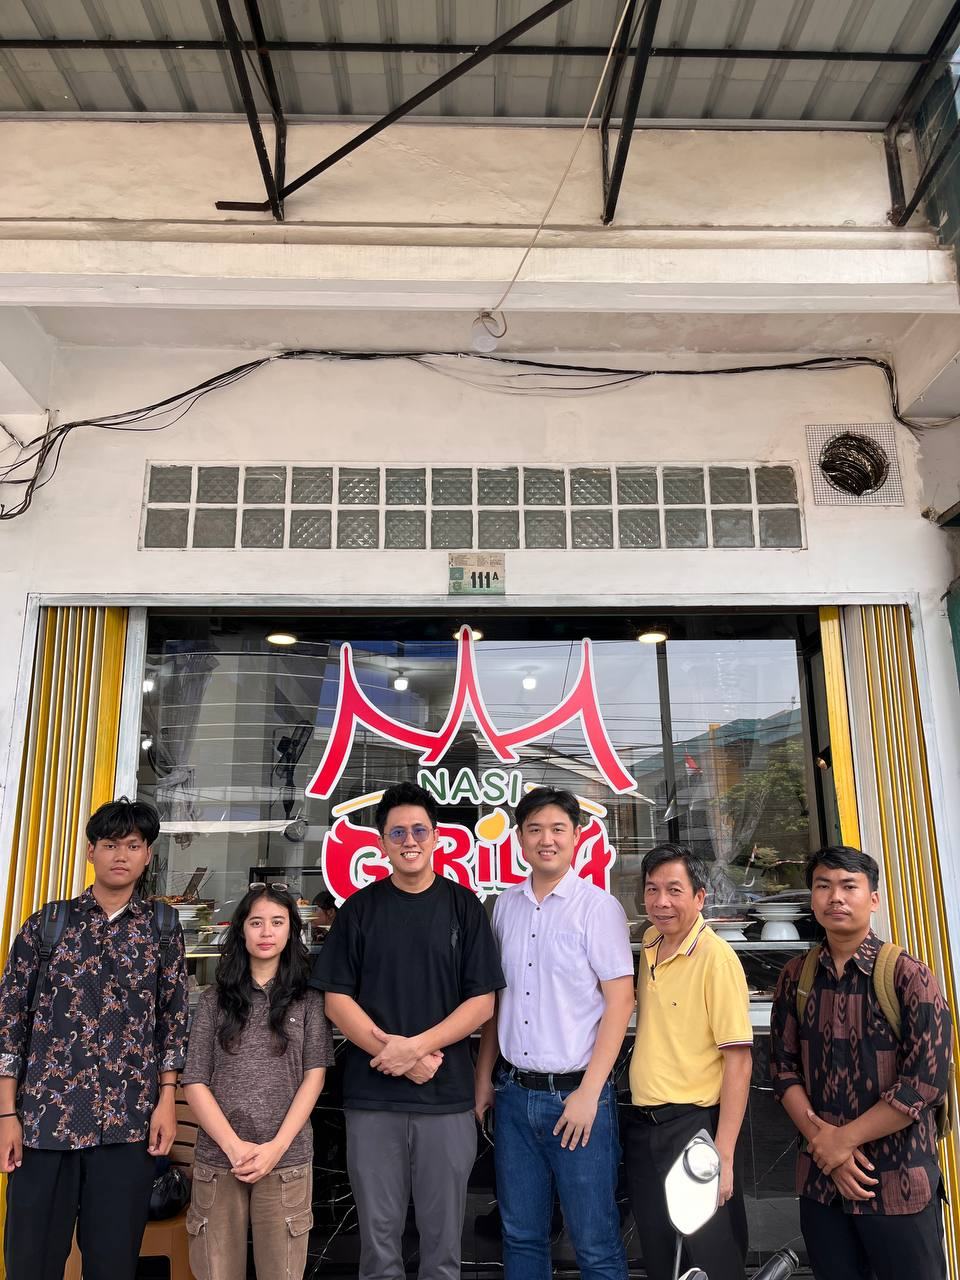
\includegraphics[width=0.78\textwidth,height=0.62\textheight,keepaspectratio]{resource/05-fieldwork/01-wawancara/20260706-wawancara-pemilik/raw/photos/W-PM-20260706-pemilik-nasi-gerilya/W-PM-20260706-foto-01-dokumentasi-bersama-pemilik.jpg}
    \figuresource[0.88\textwidth]{Dokumentasi lapangan bersama pemilik Nasi Gerilya; diolah peneliti (2026).}
    \caption{Dokumentasi Bersama Pemilik Nasi Gerilya}
    \label{fig:dokumentasi-pemilik-nasi-gerilya}
\end{figure}

\FloatBarrier

\begingroup
\scriptsize
\begin{xltabular}{\textwidth}{|C{0.7cm}|L{3.1cm}|Y|}
\caption{Rekap Pokok Temuan Wawancara Kompetitor}
\label{tab:rekap-wawancara-kompetitor} \\
\toprule
\textbf{No.} & \textbf{Informan} & \textbf{Pokok Temuan} \\ \hline
\midrule
\endfirsthead

\continuedtabletitle{3}
\toprule
\textbf{No.} & \textbf{Informan} & \textbf{Pokok Temuan} \\ \hline
\midrule
\endhead

\continuedtablefooter{3}
\endfoot

\bottomrule
\endlastfoot

1 & Kasir Rumah Makan Istana Krakatau & Penjualan masih didominasi pembelian langsung sekitar 80\%. Jam ramai berada pada pukul 11.30--14.00 dan 18.00--19.00. Menu online yang disebut adalah ikan sambal dengan harga sekitar Rp37 ribuan. Promo GrabFood digunakan, namun nilai voucher tidak selalu besar. Keluhan yang muncul adalah pesanan kurang lengkap, item tertinggal, dan driver menunggu. Pengecekan pesanan dilakukan langsung oleh petugas yang mem-packing. Keunggulan usaha terletak pada rasa, pelayanan cepat, porsi online, serta variasi sambal. \\ \hline
2 & Ken, Pondok Krakatau & GrabFood berkontribusi sekitar separuh pesanan. Jam ramai terjadi pada makan siang dan akhir pekan. Menu yang sering dipesan adalah ayam goreng, nasi ayam rendang, nasi ikan kakap, dan nasi ikan nila dengan harga sekitar Rp38 ribuan. Promo tersedia dari platform dan toko. Pelanggan kembali karena rasa enak dan pelayanan cepat. Kendala yang muncul meliputi stok yang belum diperbarui, porsi/rasa yang belum selalu konsisten, driver menunggu, dan item pesanan tertinggal. Pengecekan packing dilakukan melalui jumlah item, kuah, dan kelengkapan lain. \\ \hline
\end{xltabular}
\tablesource[\textwidth]{Wawancara kompetitor dengan Istana Krakatau dan Pondok Krakatau; diolah peneliti (2026).}
\endgroup

\begingroup
\scriptsize
\begin{xltabular}{\textwidth}{|C{0.7cm}|L{3.0cm}|Y|}
\caption{Rekap Pokok Temuan Wawancara Pegawai Nasi Gerilya}
\label{tab:rekap-wawancara-pegawai-nasi-gerilya} \\
\toprule
\textbf{No.} & \textbf{Informan} & \textbf{Pokok Temuan} \\ \hline
\midrule
\endfirsthead

\continuedtabletitle{3}
\toprule
\textbf{No.} & \textbf{Informan} & \textbf{Pokok Temuan} \\ \hline
\midrule
\endhead

\continuedtablefooter{3}
\endfoot

\bottomrule
\endlastfoot

1 & Bella / Laudia Sintiabula Sinalaki & Dapur memiliki pembagian kerja antara leader, senter, butcher, cook, dan helper. Proses kerja dimulai dari pengecekan stok, pengeluaran bahan, pemanasan lauk, dan pengolahan menu utama. Standar resep, takaran, laporan penjualan, dan pengecekan rasa digunakan untuk menjaga kualitas. Menu yang sering dibuat adalah ayam pop dan dendeng. Rendang membutuhkan waktu 5--6 jam, sedangkan ayam goreng membutuhkan proses marinasi. Catatan khusus seperti pemisahan kuah atau sambal masih dapat dipenuhi, tetapi permintaan masak khusus sulit dilakukan karena sistem masak massal. Kendala yang muncul meliputi pesanan mendadak, kondisi ramai, keterlambatan, komunikasi HT yang tidak selalu jelas, menu habis, serta kebutuhan penguatan SOP dan SDM. \\ \hline
2 & Ririn & Kasir berfokus pada pembayaran, sedangkan checker menangani pesanan takeaway dan online. Pesanan GrabFood masuk melalui notifikasi dan print bill, kemudian salinan pesanan ditempel pada box. Aplikasi ojek online dibuka sekitar 09.45 setelah pembaruan lauk. Menu yang sering dipesan melalui GrabFood meliputi ayam goreng, ayam pop, marlin, dan ikan. Staf merekomendasikan menu best seller kepada pelanggan baru, seperti ayam pop, dendeng, cumi, kikil, kepala ikan, dan cincang. Kendala yang muncul antara lain item berkuah rawan tertinggal, nomor pesanan mirip, driver perlu diberi estimasi tunggu, harga GrabFood dipersepsikan berbeda, promo dapat membuat order meningkat, dan komplain perlu ditangani dengan permintaan maaf atau kompensasi. Foto menu dinilai sudah sesuai, tetapi batas request pelanggan tetap perlu dijaga sesuai SOP. \\ \hline
\end{xltabular}
\tablesource[\textwidth]{Wawancara pegawai Nasi Gerilya; diolah peneliti (2026).}
\endgroup

\begingroup
\scriptsize
\begin{xltabular}{\textwidth}{|C{0.7cm}|L{3.3cm}|Y|}
\caption{Rekap Pokok Temuan Wawancara Pendamping Pengembangan Sistem}
\label{tab:rekap-wawancara-pendamping-sistem} \\
\toprule
\textbf{No.} & \textbf{Informan} & \textbf{Pokok Temuan} \\ \hline
\midrule
\endfirsthead

\continuedtabletitle{3}
\toprule
\textbf{No.} & \textbf{Informan} & \textbf{Pokok Temuan} \\ \hline
\midrule
\endhead

\continuedtablefooter{3}
\endfoot

\bottomrule
\endlastfoot

1 & Intern Business Consultant Nasi Gerilya & Pendampingan berfokus pada sistem antrean, absensi digital, menu digital, dan stamp digital. Masalah utama yang diamati adalah antrean dari jalur dine in, ojek online, dan takeaway yang belum sepenuhnya teratur. GrabFood dinilai berperan besar karena pasar ojek online Nasi Gerilya banyak berasal dari platform tersebut. Target potensial meliputi pekerja, mahasiswa, pelanggan sekitar, pelanggan jam makan siang, dan pelanggan yang terbiasa memakai ojek online. Positioning yang perlu diperkuat adalah nasi Padang Medan yang praktis, cepat, lauknya kuat, cocok untuk makan siang, mengenyangkan, dan tetap enak. Ayam pop dinilai layak menjadi hero menu. Tampilan toko digital sudah cukup baik tetapi masih dapat ditingkatkan. Prioritas perbaikan mengarah pada sistem internal yang lebih efektif, efisien, profesional, dan terdigitalisasi. \\ \hline
\end{xltabular}
\tablesource[\textwidth]{Wawancara pendamping pengembangan sistem Nasi Gerilya; diolah peneliti (2026).}
\endgroup

\FloatBarrier
\subsection*{Rekap Kode Temuan Wawancara}
\label{lamp:rekap-kode-temuan-wawancara}

Rekap berikut memuat kode temuan wawancara lapangan yang digunakan sebagai rujukan ringkas dalam Bab IV. Kode disusun menurut kelompok sumber wawancara agar temuan utama dapat dibaca kembali secara lebih lengkap.

\begingroup
\tiny
\begin{xltabular}{\textwidth}{|C{0.9cm}|L{2.15cm}|Y|L{2.4cm}|L{1.95cm}|}
\caption{Rekap Kode Temuan Wawancara Lapangan}
\label{tab:rekap-kode-temuan-wawancara-lapangan} \\
\toprule
\textbf{Kode} & \textbf{Sumber Data} & \textbf{Pokok Temuan} & \textbf{Tema} & \textbf{Kategori} \\ \hline
\midrule
\endfirsthead

\continuedtabletitle{5}
\toprule
\textbf{Kode} & \textbf{Sumber Data} & \textbf{Pokok Temuan} & \textbf{Tema} & \textbf{Kategori} \\ \hline
\midrule
\endhead

\continuedtablefooter{5}
\endfoot

\bottomrule
\endlastfoot
K01.1 & Wawancara pegawai Nasi Gerilya & Dapur memiliki pembagian kerja antara leader, senter, butcher, cook, dan helper. Aktivitas awal mencakup cek stok, mengeluarkan bahan, memanaskan lauk, dan mulai memasak menu utama. & People, process & Kekuatan \\ \hline
K01.2 & Wawancara pegawai Nasi Gerilya & Proses pesanan dari kasir ke dapur dimulai dari konfirmasi pesanan, pengecekan stok, lalu memasak sesuai jenis menu. & Process & Kekuatan \\ \hline
K01.3 & Wawancara pegawai Nasi Gerilya & Jam ramai terutama akhir pekan; pesanan mendadak dan kondisi hectic dapat membuat pesanan menumpuk. & Process & Kelemahan \\ \hline
K01.4 & Wawancara pegawai Nasi Gerilya & Keterlambatan pernah terjadi karena waktu sempit, pesanan mendadak, dan tekanan operasional. & Process, people & Kelemahan \\ \hline
K01.5 & Wawancara pegawai Nasi Gerilya & Dapur menggunakan standar resep, takaran, laporan penjualan, serta double-check rasa dan hasil akhir. & Product, process & Kekuatan \\ \hline
K01.6 & Wawancara pegawai Nasi Gerilya & Menu yang sering dibuat adalah ayam pop dan dendeng; rendang membutuhkan waktu lama dan ayam goreng membutuhkan proses marinasi. & Product & Kelemahan \\ \hline
K01.7 & Wawancara pegawai Nasi Gerilya & Catatan khusus terbatas seperti kuah atau sambal dipisah masih memungkinkan, tetapi permintaan masak khusus sulit dipenuhi karena sistem masak massal. & Product, process & Kelemahan \\ \hline
K01.8 & Wawancara pegawai Nasi Gerilya & Keluhan yang terdengar antara lain aroma kikil, menu habis, dan risiko kualitas bahan tertentu. & Product & Kelemahan \\ \hline
K01.9 & Wawancara pegawai Nasi Gerilya & Komunikasi kasir-dapur memakai HT, tetapi bisa tidak jelas saat area dapur sibuk atau tidak ada yang memegang HT. & People, process & Kelemahan \\ \hline
K01.10 & Wawancara pegawai Nasi Gerilya & Kekuatan utama menurut dapur adalah konsistensi rasa, sedangkan perbaikan utama terkait SOP, SDM, pelayanan floor, dan kecepatan packing. & Product, people, process & Kelemahan \\ \hline
K01.11 & Wawancara pegawai Nasi Gerilya & Kasir berfokus pada pembayaran, sedangkan checker menerima pesanan take away dan pesanan online. & People, process & Kekuatan \\ \hline
K01.12 & Wawancara pegawai Nasi Gerilya & Staf merekomendasikan menu best seller kepada pelanggan baru dan menyesuaikan rekomendasi dengan preferensi pelanggan. & Product, people & Kekuatan \\ \hline
K01.13 & Wawancara pegawai Nasi Gerilya & Aplikasi ojek online dibuka sekitar 09.45; sebelum itu staf wajib memperbarui lauk secara berkala. & Place, process & Kekuatan \\ \hline
K01.14 & Wawancara pegawai Nasi Gerilya & Pesanan GrabFood masuk melalui notifikasi dan print bill; checker menempelkan salinan pesanan pada box. & Process & Kekuatan \\ \hline
K01.15 & Wawancara pegawai Nasi Gerilya & Item basah atau berkuah yang dipisah dari nasi rawan tertinggal, terutama saat kondisi ramai. & Process & Kelemahan \\ \hline
K01.16 & Wawancara pegawai Nasi Gerilya & Nomor GrabFood yang mirip dan driver salah menyebut nomor dapat menyebabkan risiko pesanan tertukar. & Process, place & Kelemahan \\ \hline
K01.17 & Wawancara pegawai Nasi Gerilya & Driver diberi nomor antrean dan staf perlu memberi estimasi tunggu ketika makanan belum selesai. & Process, people & Kelemahan \\ \hline
K01.18 & Wawancara pegawai Nasi Gerilya & Menu yang sering dipesan melalui GrabFood adalah ayam goreng, ayam pop, marlin, dan ikan; kepala ikan cenderung untuk momen tertentu. & Product & Kekuatan \\ \hline
K01.19 & Wawancara pegawai Nasi Gerilya & Harga GrabFood berbeda dari take away dan sesekali dianggap mahal; promo membuat pelanggan membandingkan harga lalu memilih GrabFood. & Price, promotion & Kelemahan \\ \hline
K01.20 & Wawancara pegawai Nasi Gerilya & Promo menyebabkan order membeludak dan harus diinformasikan ke dapur agar stok menu promo siap. & Promotion, process & Kelemahan \\ \hline
K01.21 & Wawancara pegawai Nasi Gerilya & Komplain meliputi porsi ikan, aroma kikil, tingkat pedas, dan makanan yang dianggap bermasalah; respons dilakukan dengan permintaan maaf dan kompensasi. & Product, process, people & Kelemahan \\ \hline
K01.22 & Wawancara pegawai Nasi Gerilya & Foto menu dinilai sudah sesuai dan opsi pesanan cukup banyak, tetapi batas request pelanggan tetap perlu dijaga sesuai SOP. & Physical evidence, product & Kekuatan \\ \hline
K02.1 & Wawancara intern business consultant Nasi Gerilya & Informan adalah mahasiswa magang IT/Sistem Informasi melalui APINDO UMKM Merdeka yang berfokus pada sistem antrean, absensi digital, menu digital, dan stamp digital. & People, process & Kekuatan \\ \hline
K02.2 & Wawancara intern business consultant Nasi Gerilya & Tujuan pendampingan adalah merapikan proses internal agar kerja lebih efektif, efisien, profesional, dan terdigitalisasi. & Process, people & Kekuatan \\ \hline
K02.3 & Wawancara intern business consultant Nasi Gerilya & Keterlibatan informan mencakup observasi kebutuhan operasional, identifikasi kendala lapangan, pembuatan sistem, dan memastikan sistem dapat berjalan. & Process, people & Kekuatan \\ \hline
K02.4 & Wawancara intern business consultant Nasi Gerilya & Data pendampingan berasal dari observasi outlet, jam ramai GrabFood, harga jual GrabFood, pola antrean, kebutuhan karyawan, dan diskusi dengan Nasi Gerilya. & Research input, process & Kekuatan \\ \hline
K02.5 & Wawancara intern business consultant Nasi Gerilya & Masalah utama adalah antrean belum teratur dari tiga jalur; menu digital dan stamp digital dibuat untuk mengurangi beban pencatatan manual dan membangun loyalitas. & Process, promotion, physical evidence & Kelemahan \\ \hline
K02.6 & Wawancara intern business consultant Nasi Gerilya & GrabFood memiliki peran sangat besar karena pasar ojek online terbesar Nasi Gerilya banyak berasal dari GrabFood dan ordernya cukup tinggi. & Place & Peluang \\ \hline
K02.7 & Wawancara intern business consultant Nasi Gerilya & Target potensial adalah pekerja, mahasiswa, pelanggan sekitar, pelanggan jam makan siang, dan pelanggan yang terbiasa memakai ojek online. & STP, place & Peluang \\ \hline
K02.8 & Wawancara intern business consultant Nasi Gerilya & Positioning yang perlu diperkuat adalah nasi Padang Medan yang praktis, cepat, lauknya kuat, cocok untuk makan siang, mengenyangkan, dan tetap enak. & Positioning, product & Kekuatan \\ \hline
K02.9 & Wawancara intern business consultant Nasi Gerilya & Ayam pop dinilai layak menjadi hero menu untuk menarik perhatian pelanggan online. & Product, positioning & Kekuatan \\ \hline
K02.10 & Wawancara intern business consultant Nasi Gerilya & Harga dan promo GrabFood dinilai cukup baik, tetapi diskon atau voucher perlu dihitung agar tidak mengganggu margin, harga jual, dan HPP. & Price, promotion & Kelemahan \\ \hline
K02.11 & Wawancara intern business consultant Nasi Gerilya & Tampilan toko digital sudah cukup baik tetapi masih dapat ditingkatkan; menu digital membuat pengalaman pelanggan lebih praktis dan modern. & Physical evidence, process & Peluang \\ \hline
K02.12 & Wawancara intern business consultant Nasi Gerilya & Promosi penting untuk mendukung sistem digital, terutama agar pelanggan mengetahui menu digital, stamp digital, dan program loyalitas. & Promotion, loyalty & Peluang \\ \hline
K02.13 & Wawancara intern business consultant Nasi Gerilya & Kompetitor relevan menurut informan adalah Pondok Gurih karena sama-sama menyasar pelanggan makanan berat dan lauk khas. & Competition, positioning & Ancaman \\ \hline
K02.14 & Wawancara intern business consultant Nasi Gerilya & Pembeda utama Nasi Gerilya adalah rasa lauk kuat, jumlah pelanggan yang besar, dan kemauan UMKM untuk berbenah melalui sistem digital. & Product, process, differentiation & Kekuatan \\ \hline
K02.15 & Wawancara intern business consultant Nasi Gerilya & Kendala layanan paling berpengaruh terjadi saat makan siang, hari Minggu, dan hari raya ketika pesanan banyak kanal masuk bersamaan dan koordinasi menjadi sulit. & Process, people & Kelemahan \\ \hline
K02.16 & Wawancara intern business consultant Nasi Gerilya & Kelemahan utama adalah pengelolaan data pelanggan dan layanan dine in yang perlu lebih rapi agar usaha tidak hanya bergantung pada platform online. & Promotion, process, loyalty & Kelemahan \\ \hline
K02.17 & Wawancara intern business consultant Nasi Gerilya & Peluang berasal dari kebutuhan makanan cepat, praktis, dan mengenyangkan; ancaman berasal dari persaingan kuliner, biaya platform, kenaikan bahan baku, ekonomi tidak stabil, dan sensitivitas harga. & Opportunity/threat, price & Ancaman \\ \hline
K02.18 & Wawancara intern business consultant Nasi Gerilya & Indikator evaluasi yang relevan adalah jumlah pesanan, omzet, waktu pelayanan, antrean tertangani, repeat order, rating, jumlah komplain, dan efektivitas sistem. & Control, performance & Rekomendasi \\ \hline
K02.19 & Wawancara intern business consultant Nasi Gerilya & Prioritas strategi adalah membuat sistem internal lebih rapi, efektif, efisien, dan profesional melalui sistem antrean, menu digital, stamp digital, dan absensi. & Process, people & Rekomendasi \\ \hline
K02.20 & Wawancara intern business consultant Nasi Gerilya & Rekomendasi terkuat adalah sistem antrean karena masalahnya terlihat langsung; menu digital dan stamp digital relevan tetapi perlu diuji bertahap. & Process, physical evidence, loyalty & Rekomendasi \\ \hline
K02.21 & Wawancara intern business consultant Nasi Gerilya & Strategi Nasi Gerilya tidak hanya soal promosi atau GrabFood; internal yang rapi akan membuat layanan lebih cepat, pelanggan nyaman, dan pemasaran lebih berdampak pada penjualan. & Process, strategy & Rekomendasi \\ \hline
K09.1 & Wawancara pemilik Nasi Gerilya & Komposisi pembelian diperkirakan GrabFood sekitar 50\%, GoFood 12\%, ShopeeFood 8\%, dan offline 30\%. & Place, channel mix & Kekuatan \\ \hline
K09.2 & Wawancara pemilik Nasi Gerilya & Pemasok berasal dari jaringan yang biasa mengirim ke supermarket; bumbu dan sayur dipilih langsung serta dikirim dengan cold storage. & Product, supplier quality & Kekuatan \\ \hline
K09.3 & Wawancara pemilik Nasi Gerilya & Penyimpanan bahan menggunakan freezer peti dan lemari chiller untuk sayur. & Product, process & Kekuatan \\ \hline
K09.4 & Wawancara pemilik Nasi Gerilya & Konsistensi rasa dijaga ketat; pemilik pernah membuang batch rendang ketika urutan masuk rempah membuat rasa berubah. & Product, quality control & Kekuatan \\ \hline
K09.5 & Wawancara pemilik Nasi Gerilya & Margin tidak dibuka karena rahasia; keuntungan belum cukup untuk BEP dan rencana dapur central serta cabang Medan membutuhkan peningkatan keuntungan. & Price, finance & Kelemahan \\ \hline
K09.6 & Wawancara pemilik Nasi Gerilya & Dapur dan frontline memiliki leader masing-masing; leader frontline mengelola GrabFood dan data dikirim ke admin di unit Sambal Gerilya. & People, process & Kekuatan \\ \hline
K09.7 & Wawancara pemilik Nasi Gerilya & Pemasaran melalui KOL makanan pernah dicoba dengan hasil bervariasi tetapi secara keseluruhan membantu penjualan. & Promotion & Peluang \\ \hline
K09.8 & Wawancara pemilik Nasi Gerilya & Kerja sama APINDO menghadirkan mahasiswa magang sebagai business consultant untuk brainstorming pemasaran dan pengembangan usaha. & People, promotion & Peluang \\ \hline
K09.9 & Wawancara pemilik Nasi Gerilya & Toko berstatus halal, meraih Rising Star GrabFood 2025 dan 2026, serta disebut sebagai restoran bintang lima di GrabFood. & Physical evidence, reputation & Kekuatan \\ \hline
K09.10 & Wawancara pemilik Nasi Gerilya & Usaha sedang mengembangkan Flowie untuk mengecek stok dan HPP di toko. & Process, technology & Kekuatan \\ \hline
K09.11 & Wawancara pemilik Nasi Gerilya & Leader diajarkan independen agar dapat bekerja tanpa campur tangan langsung pemilik. & People & Kekuatan \\ \hline
K09.12 & Wawancara pemilik Nasi Gerilya & Regenerasi dilakukan dengan mendidik wakil leader. & People & Kekuatan \\ \hline
K03.1 & Wawancara kompetitor & GrabFood menyumbang sekitar lebih kurang 50 persen dari total pesanan Pondok Krakatau. & Place & Ancaman \\ \hline
K03.2 & Wawancara kompetitor & Jam ramai Pondok Krakatau berada pada makan siang dan akhir pekan. & Place, process & Ancaman \\ \hline
K03.3 & Wawancara kompetitor & Menu sering dipesan di Pondok Krakatau adalah ayam goreng, nasi ayam rendang, nasi ikan kakap, dan nasi ikan nila dengan harga sekitar Rp38 ribuan. & Product, price & Ancaman \\ \hline
K03.4 & Wawancara kompetitor & Pelanggan kembali karena rasa enak dan pelayanan cepat. & Product, people, process & Ancaman \\ \hline
K03.5 & Wawancara kompetitor & Promo tersedia dari GrabFood dan kadang dibuat oleh toko. & Promotion, price & Ancaman \\ \hline
K03.6 & Wawancara kompetitor & Stok habis kadang belum diperbarui di platform ketika pelanggan sudah order. & Process, place & Peluang \\ \hline
K03.7 & Wawancara kompetitor & Porsi dan rasa kadang tidak konsisten karena petugas bungkus atau masak berbeda. & Product, people & Peluang \\ \hline
K03.8 & Wawancara kompetitor & Pesanan kadang tertinggal, lalu dikirim ulang melalui Grab untuk disusulkan. & Process & Peluang \\ \hline
K03.9 & Wawancara kompetitor & Pengecekan packing dilakukan melalui jumlah item, kuah, dan kelengkapan lain. & Process & Ancaman \\ \hline
K03.10 & Wawancara kompetitor & Penjualan Istana Krakatau masih didominasi offline sekitar 80 persen. & Place & Ancaman \\ \hline
K03.11 & Wawancara kompetitor & Jam ramai Istana Krakatau terjadi pada 11.30--14.00 dan sekitar 18.00--19.00. & Place, process & Ancaman \\ \hline
K03.12 & Wawancara kompetitor & Menu online yang disebut adalah ikan sambal dengan harga sekitar Rp37 ribuan. & Product, price & Ancaman \\ \hline
K03.13 & Wawancara kompetitor & Pelanggan memilih Istana Krakatau karena rasa dan pelayanan cepat. & Product, process & Ancaman \\ \hline
K03.14 & Wawancara kompetitor & Promo sering dipakai terutama di GrabFood, walaupun voucher disebut tidak besar. & Promotion & Ancaman \\ \hline
K03.15 & Wawancara kompetitor & Pesanan kurang lengkap menjadi keluhan pelanggan. & Process & Peluang \\ \hline
K03.16 & Wawancara kompetitor & Pesanan tertinggal membuat driver lama menunggu. & Process & Peluang \\ \hline
K03.17 & Wawancara kompetitor & Pengecekan dilakukan langsung oleh petugas yang mem-packing. & Process & Ancaman \\ \hline
K03.18 & Wawancara kompetitor & Keunggulan Istana Krakatau ada pada sambal empat jenis, terutama sambal Padang, serta rasa dan porsi online yang lebih besar. & Product & Ancaman \\ \hline
\end{xltabular}
\tablesource[\textwidth]{Wawancara lapangan 1--4 Juli 2026; diolah peneliti (2026).}
\endgroup

\subsection*{Dokumentasi Wawancara Kompetitor Istana Krakatau}

Dokumentasi berikut memperlihatkan suasana wawancara lapangan dan kondisi pendukung pada Rumah Makan Istana Krakatau. Data ini digunakan sebagai pelengkap catatan wawancara kompetitor dalam membaca layanan, tampilan usaha, dan konteks pembanding GrabFood.

\begin{figure}[!p]
    \centering
    \begin{minipage}[t]{0.48\textwidth}
        \centering
        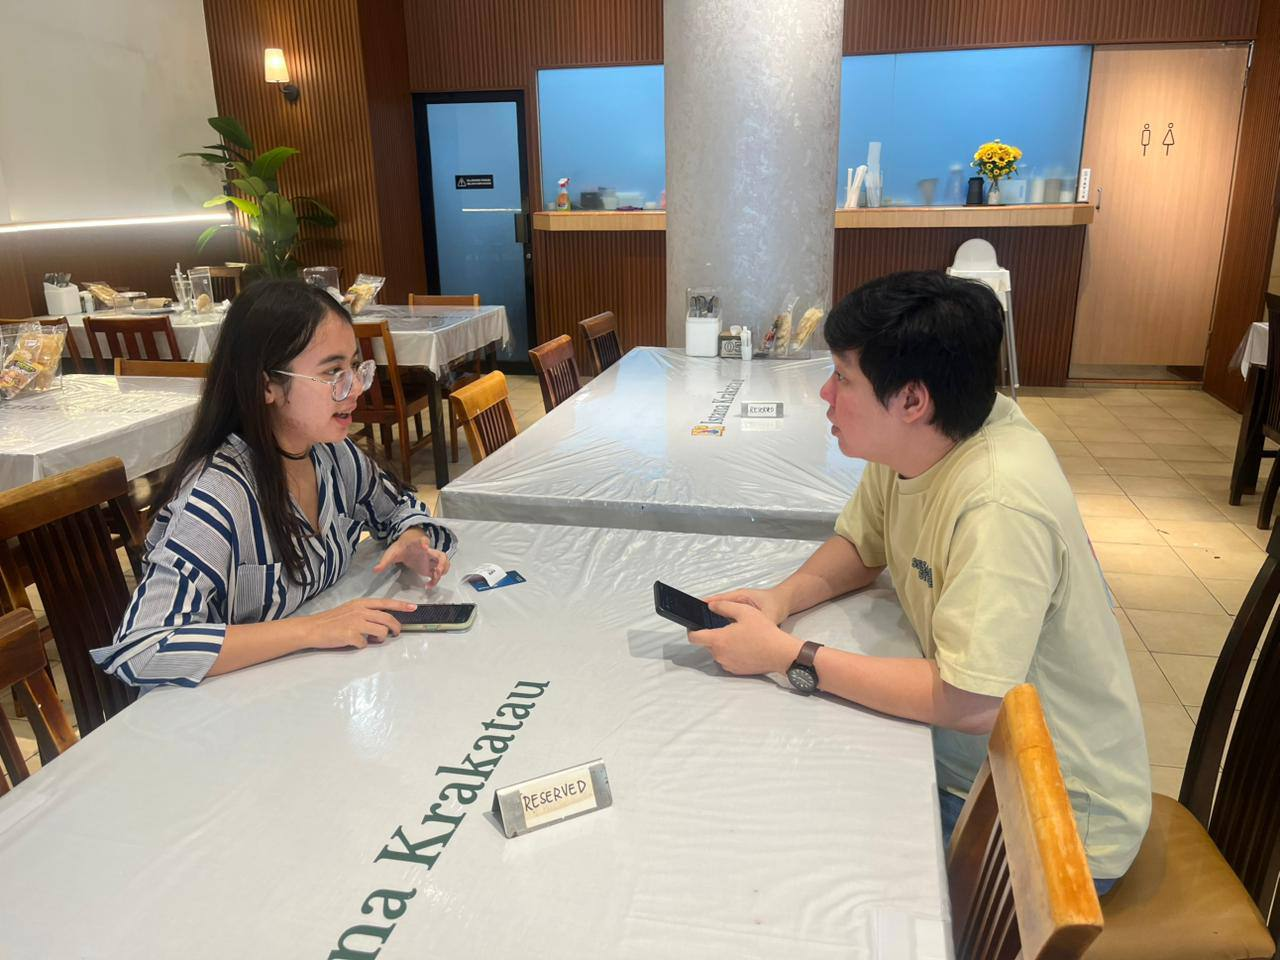
\includegraphics[width=\linewidth,height=0.30\textheight,keepaspectratio]{resource/05-fieldwork/01-wawancara/20260701-20260704-wawancara-lapangan/raw/photos/K03-PB-20260703-istana-krakatau/K03-PB-20260703-foto-01-suasana-wawancara.jpg}
        \par\footnotesize (a) Suasana wawancara kompetitor
    \end{minipage}\hfill
    \begin{minipage}[t]{0.48\textwidth}
        \centering
        
\includegraphics[width=\linewidth,height=0.30\textheight,keepaspectratio]{resource/05-fieldwork/01-wawancara/20260701-20260704-wawancara-lapangan/raw/photos/K03-PB-20260703-istana-krakatau/K03-PB-20260703-foto-02-plakat-grab.jpg}
        \par\footnotesize (b) Atribut reputasi layanan
    \end{minipage}

    \vspace{6pt}

    \begin{minipage}[t]{0.48\textwidth}
        \centering
        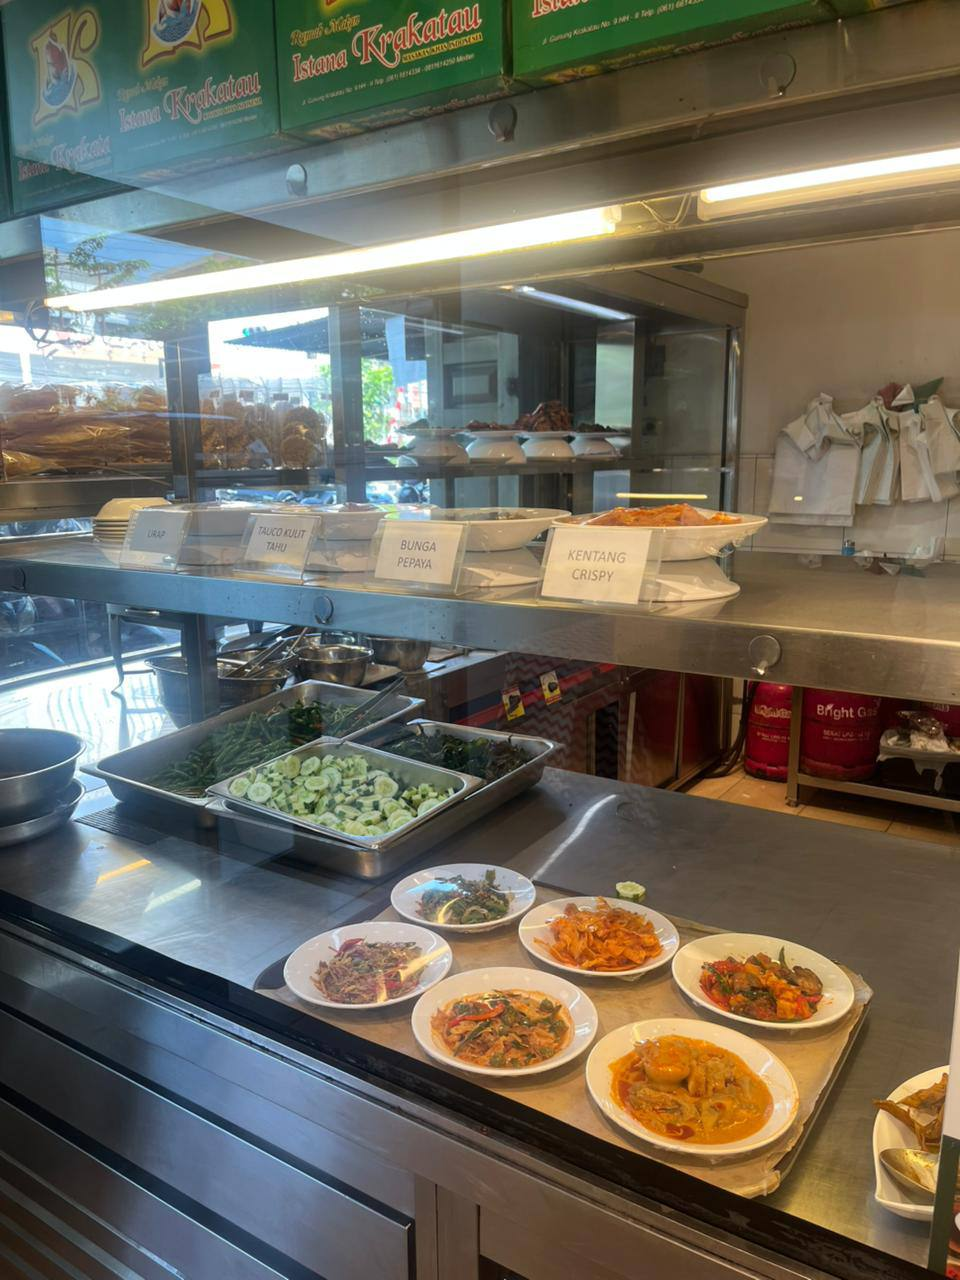
\includegraphics[width=\linewidth,height=0.30\textheight,keepaspectratio]{resource/05-fieldwork/01-wawancara/20260701-20260704-wawancara-lapangan/raw/photos/K03-PB-20260703-istana-krakatau/K03-PB-20260703-foto-03-etalase-lauk.jpg}
        \par\footnotesize (c) Etalase lauk
    \end{minipage}\hfill
    \begin{minipage}[t]{0.48\textwidth}
        \centering
        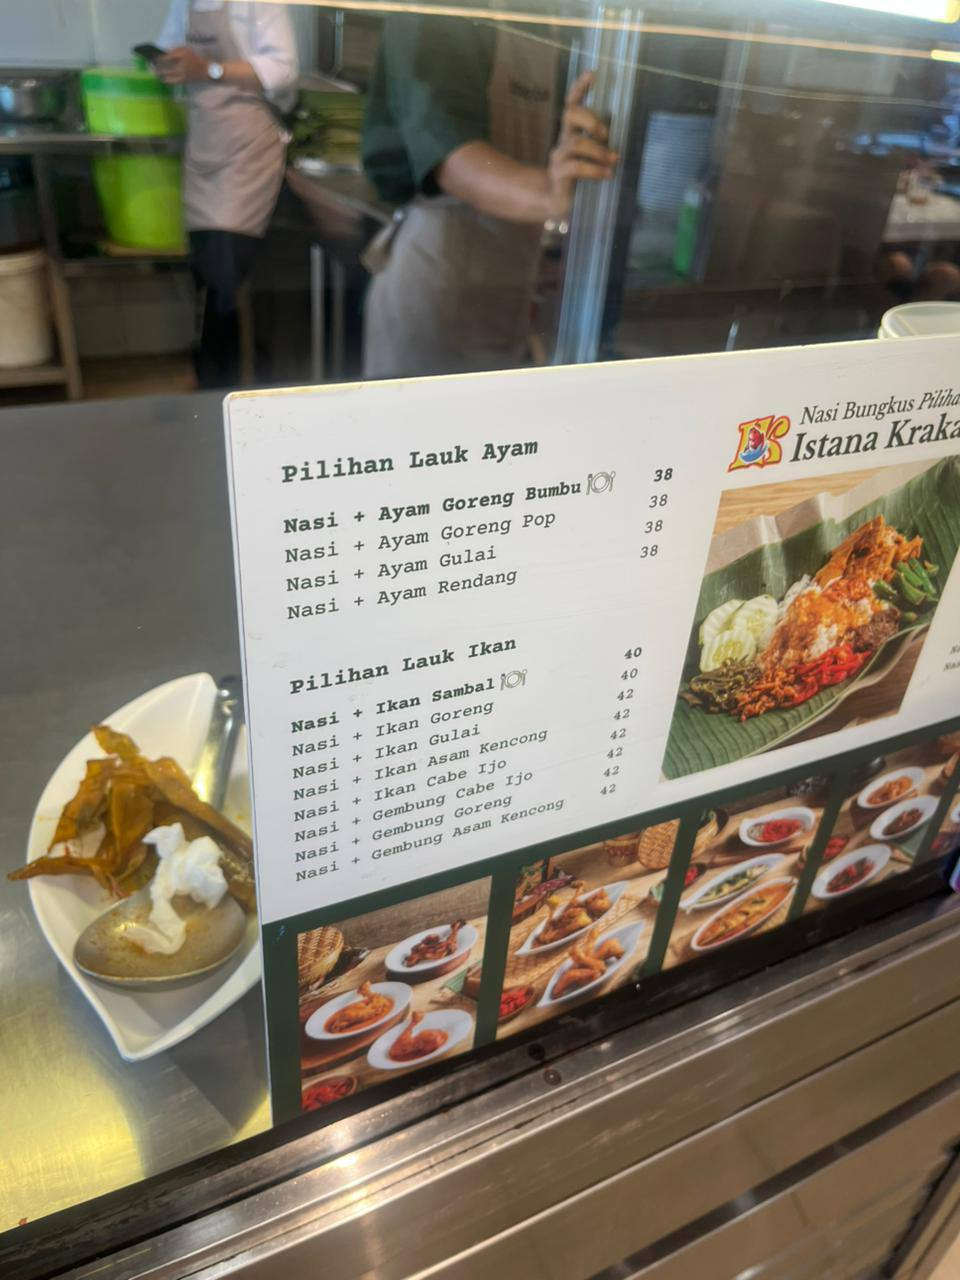
\includegraphics[width=\linewidth,height=0.30\textheight,keepaspectratio]{resource/05-fieldwork/01-wawancara/20260701-20260704-wawancara-lapangan/raw/photos/K03-PB-20260703-istana-krakatau/K03-PB-20260703-foto-04-menu-paket.jpg}
        \par\footnotesize (d) Menu paket
    \end{minipage}
    \figuresource[0.98\textwidth]{Dokumentasi lapangan pada Rumah Makan Istana Krakatau; diolah peneliti (2026).}
    \caption{Dokumentasi Wawancara Kompetitor di Rumah Makan Istana Krakatau}
    \label{fig:dokumentasi-wawancara-istana-krakatau}
\end{figure}

\FloatBarrier
\subsection*{Dokumentasi Wawancara Kompetitor Pondok Krakatau}

Dokumentasi berikut memperlihatkan situasi pengumpulan data lapangan pada Pondok Krakatau, mencakup interaksi dengan narasumber serta konteks menu yang terlihat di lokasi wawancara. Dokumentasi ini digunakan sebagai pelengkap catatan wawancara kompetitor Pondok Krakatau.
\begin{figure}[!hbp]
    \centering
    \setlength{\abovecaptionskip}{4pt}
    \setlength{\belowcaptionskip}{0pt}
    \begin{minipage}[t]{0.47\textwidth}
        \centering
        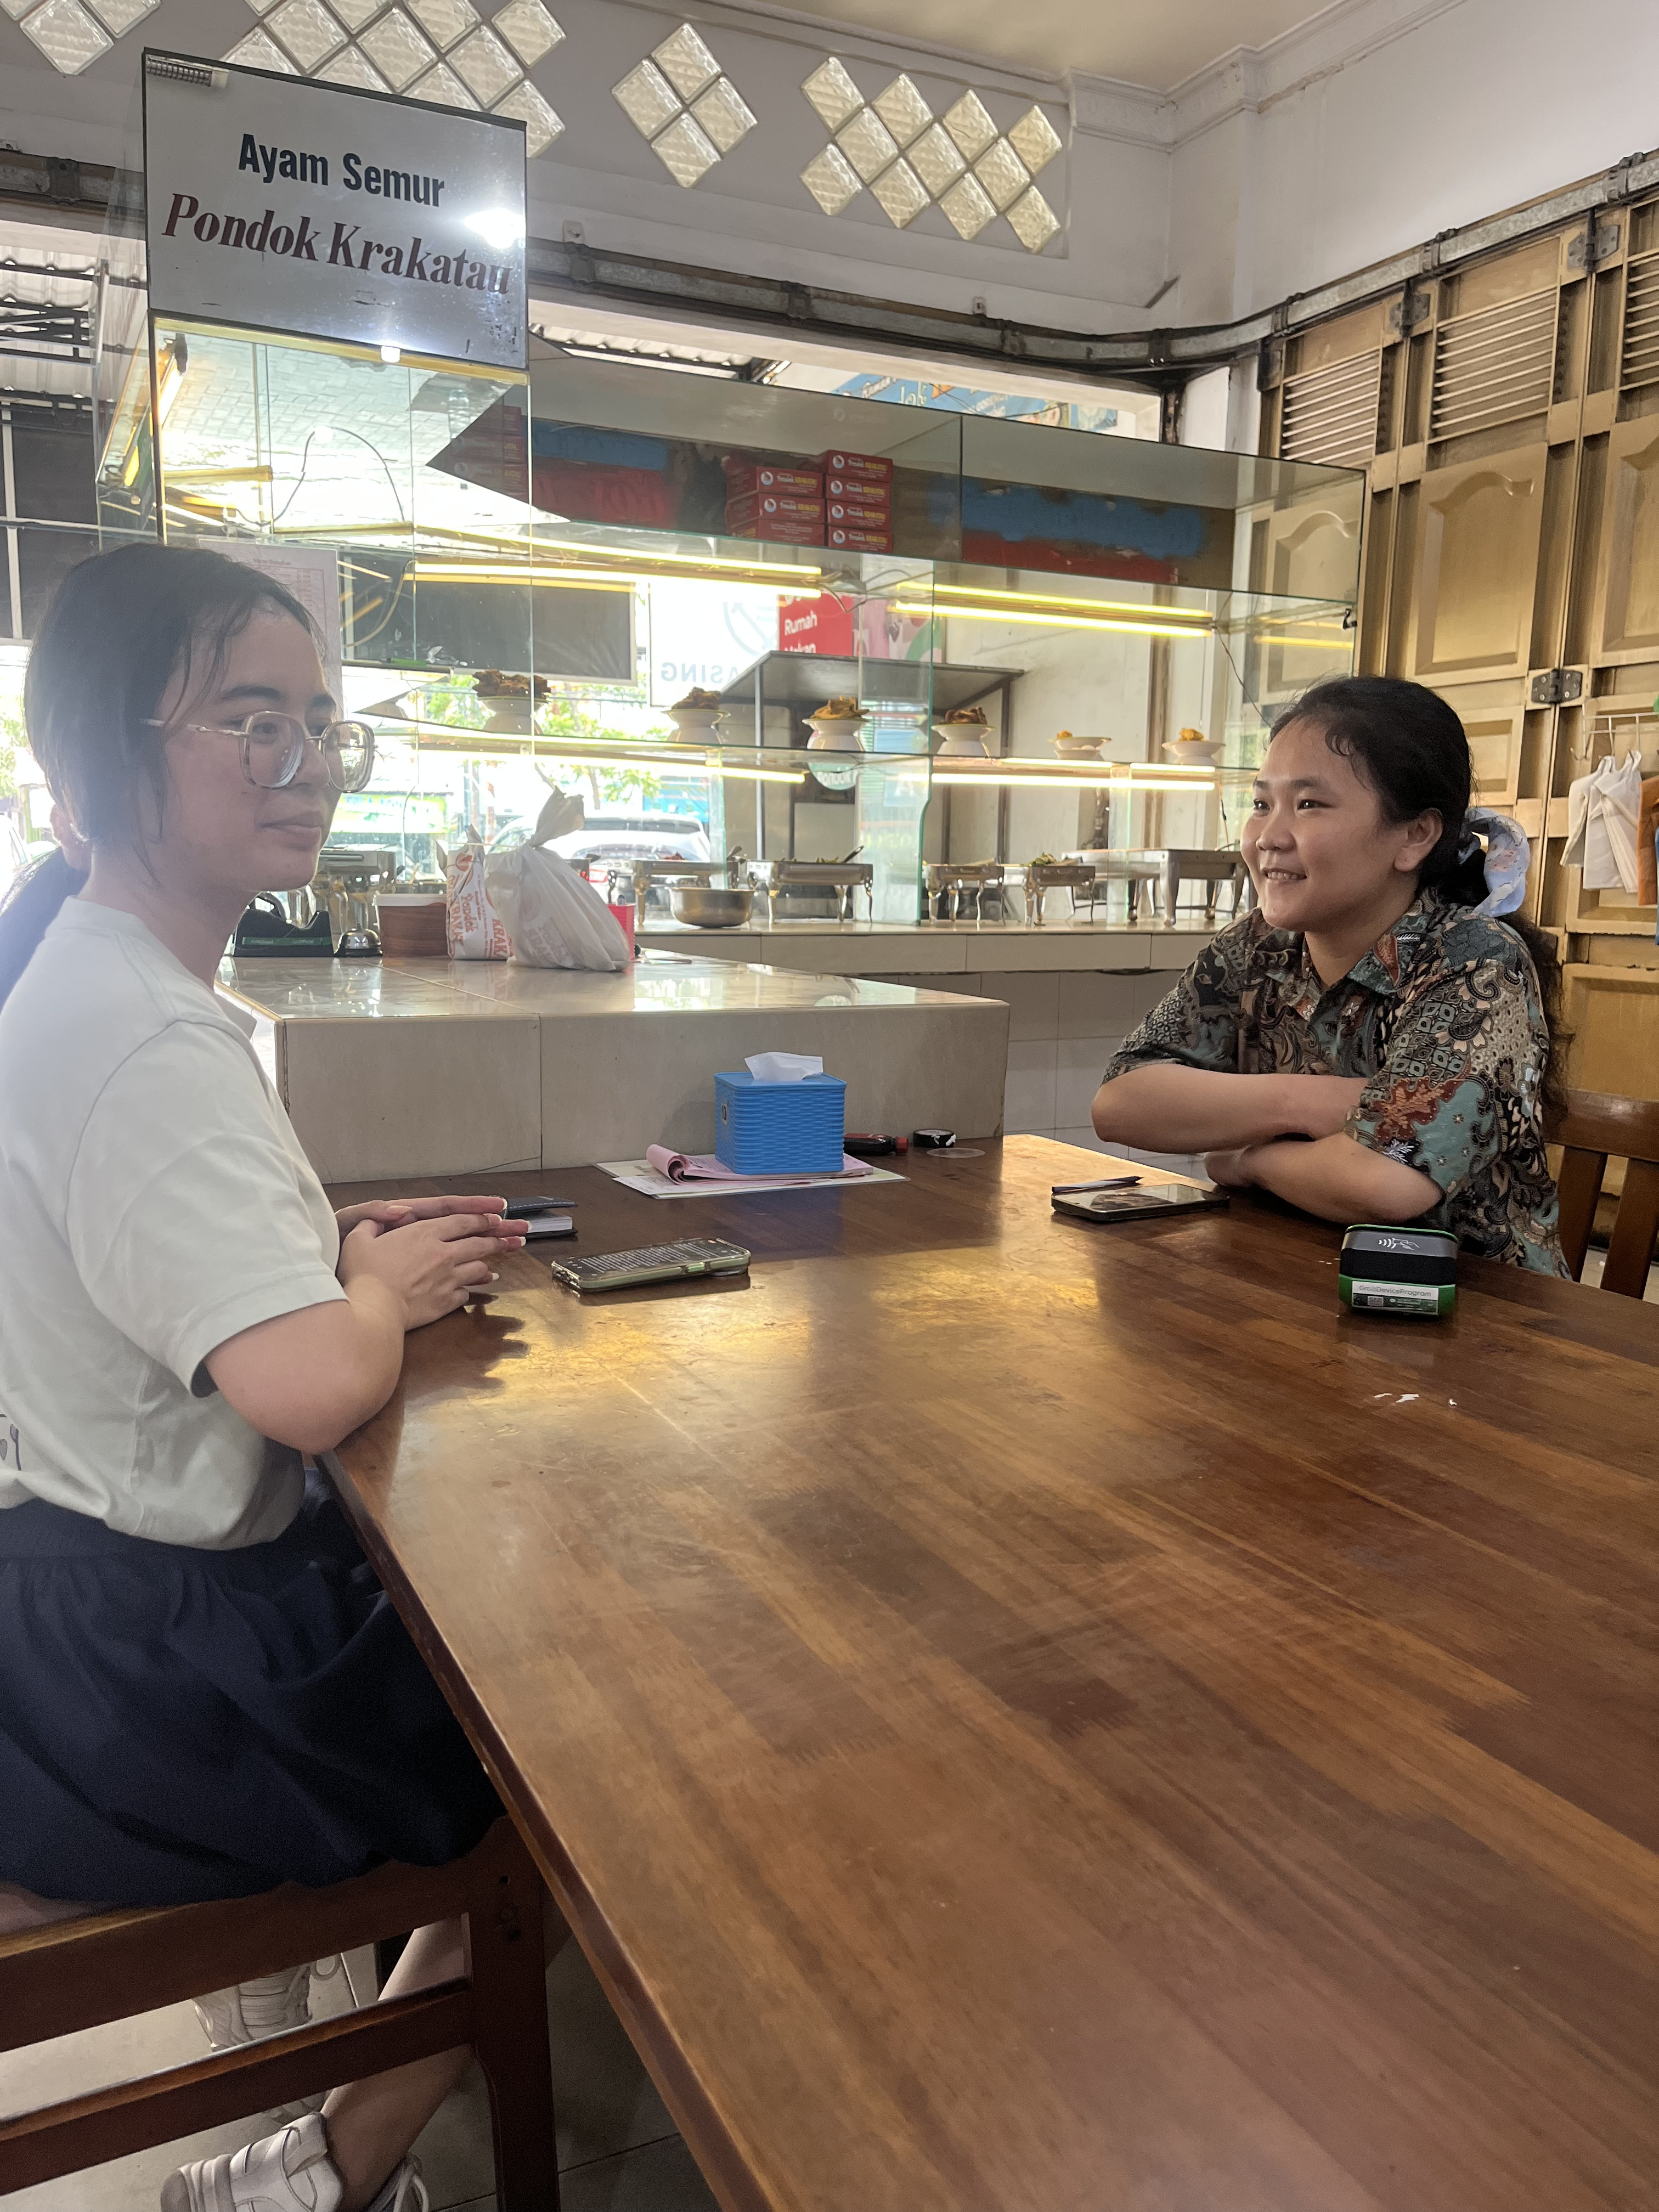
\includegraphics[width=\linewidth,height=0.245\textheight,keepaspectratio]{resource/05-fieldwork/01-wawancara/20260701-20260704-wawancara-lapangan/raw/photos/K03-PA-20260703-pondok-krakatau/K03-PA-20260703-foto-12.jpg}
        \par\vspace{2pt}\footnotesize (a) Dokumentasi kegiatan wawancara dengan narasumber
    \end{minipage}\hfill
    \begin{minipage}[t]{0.47\textwidth}
        \centering
        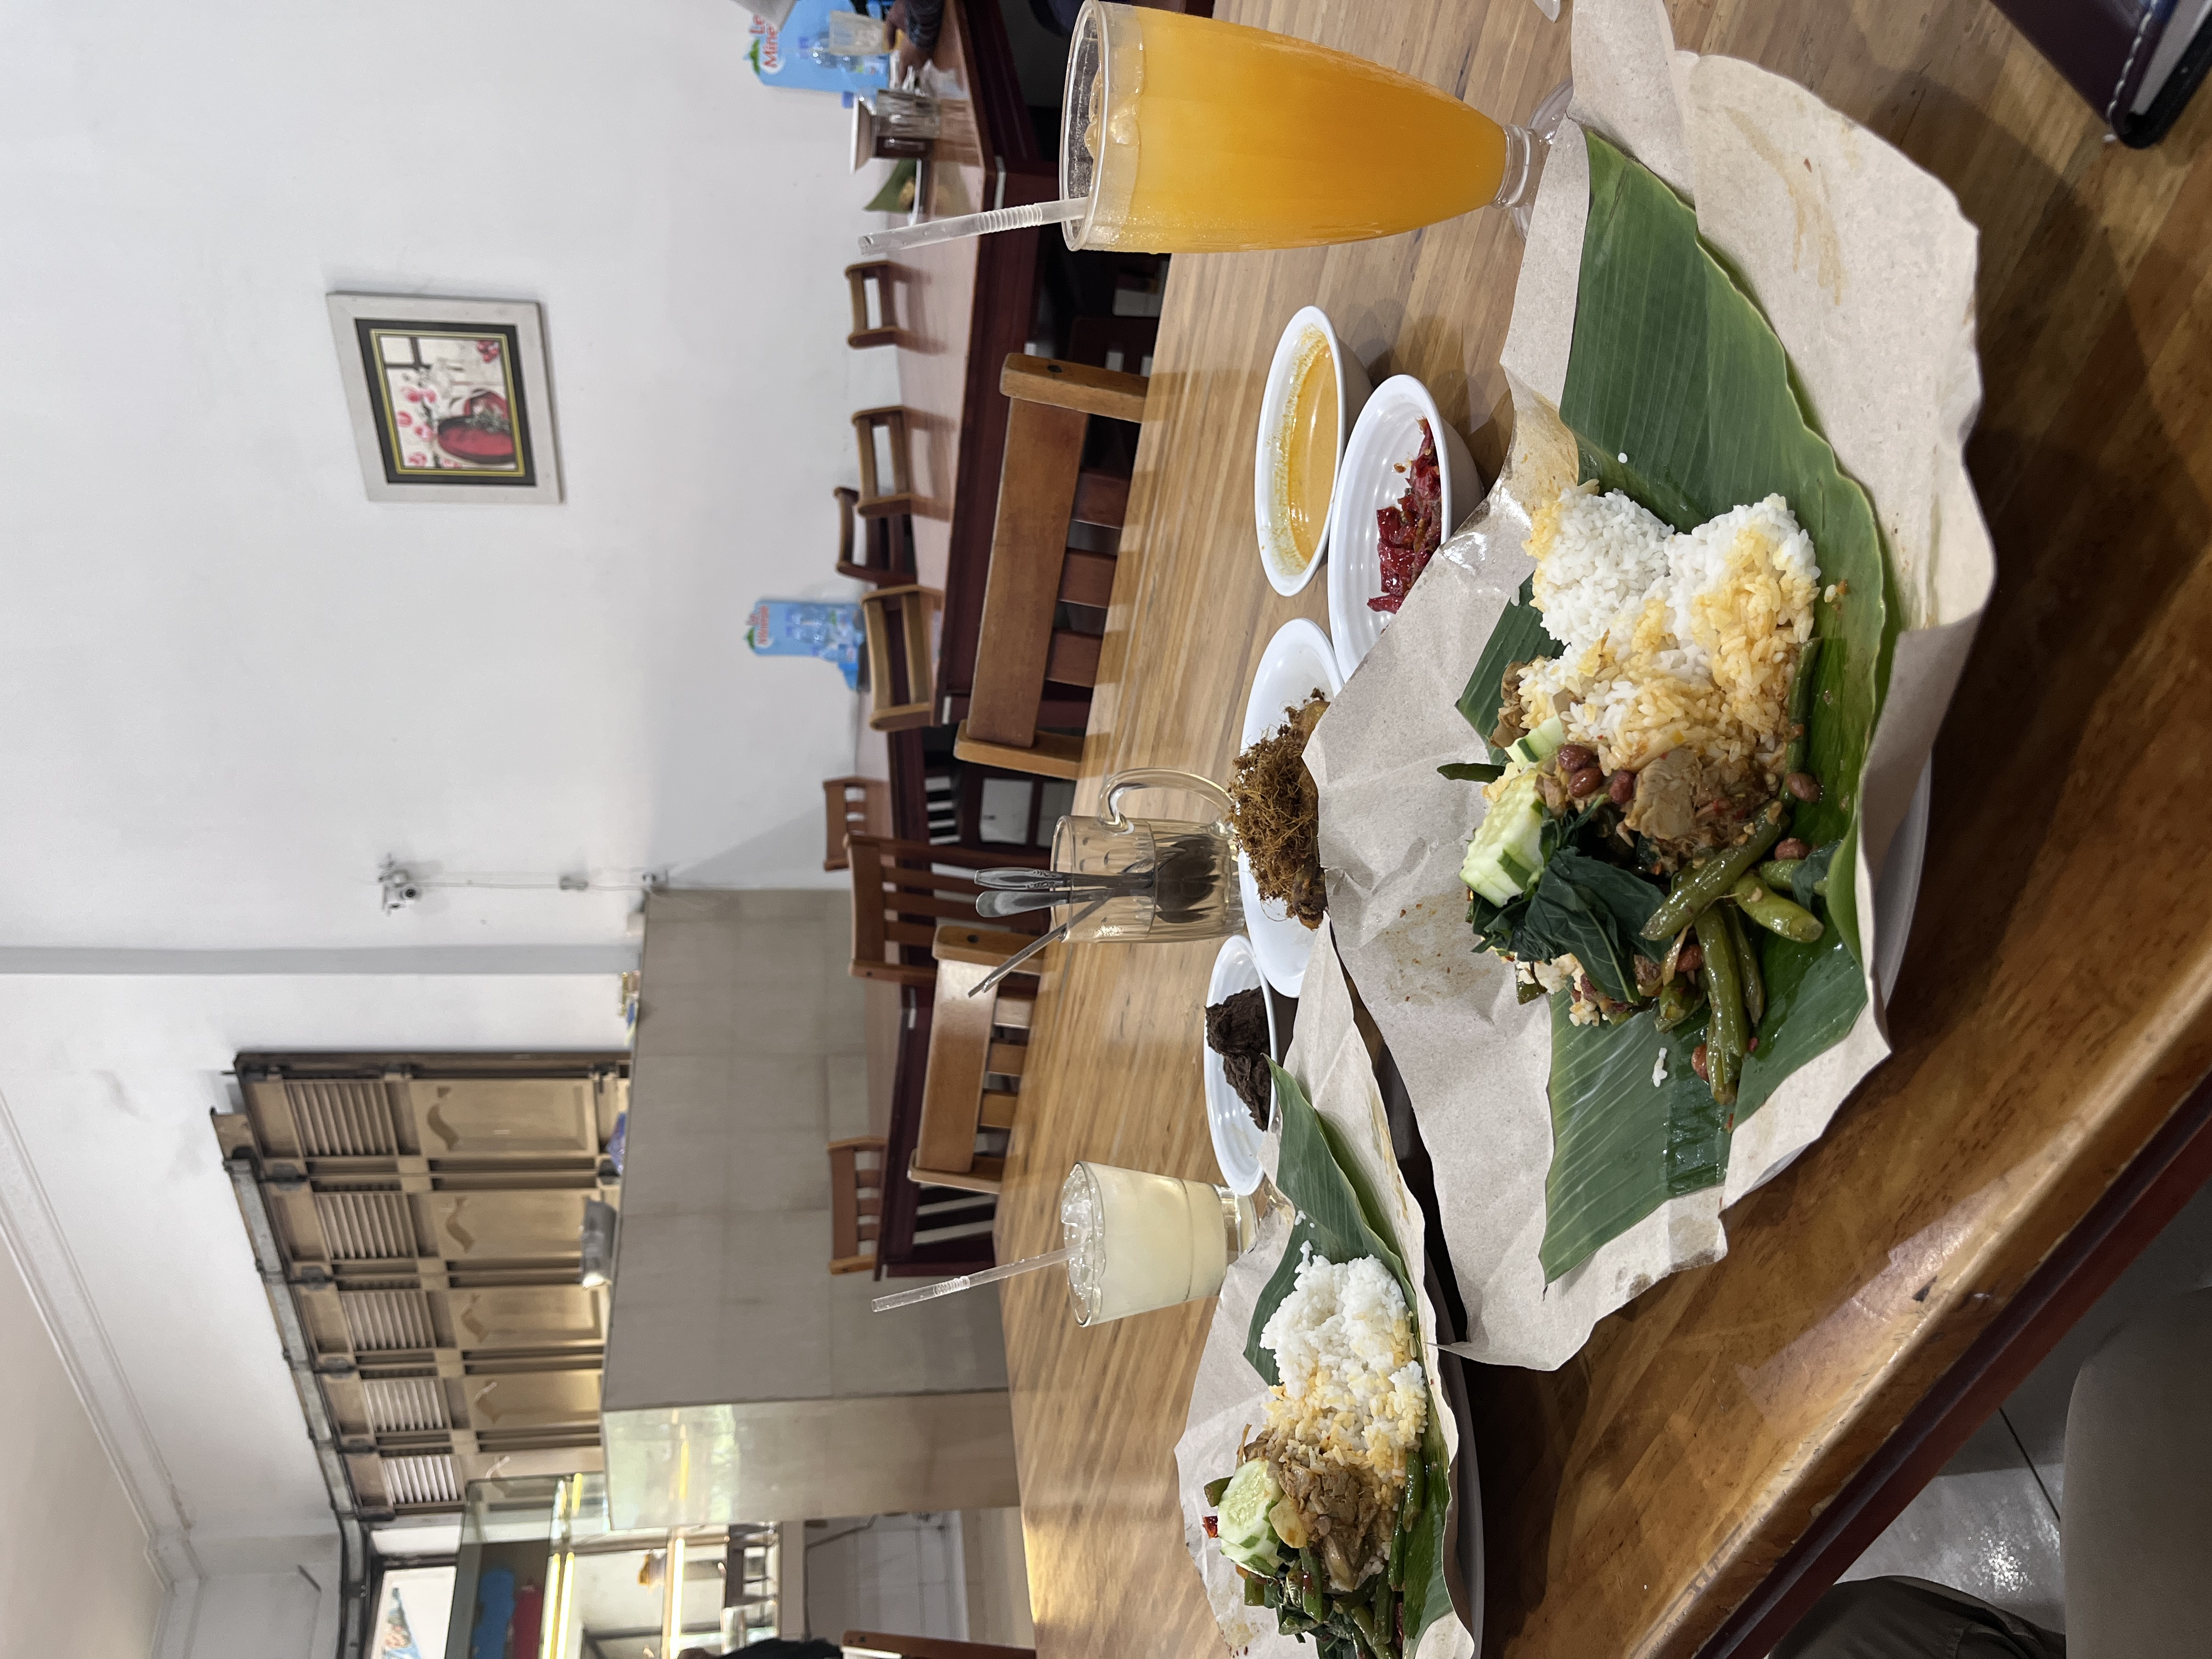
\includegraphics[angle=-90,origin=c,width=\linewidth,height=0.245\textheight,keepaspectratio]{resource/05-fieldwork/01-wawancara/20260701-20260704-wawancara-lapangan/raw/photos/K03-PA-20260703-pondok-krakatau/K03-PA-20260703-foto-07.jpg}
        \par\vspace{2pt}\footnotesize (b) Suasana interaksi di lokasi penelitian
    \end{minipage}

    \vspace{4pt}

    \begin{minipage}[t]{0.47\textwidth}
        \centering
        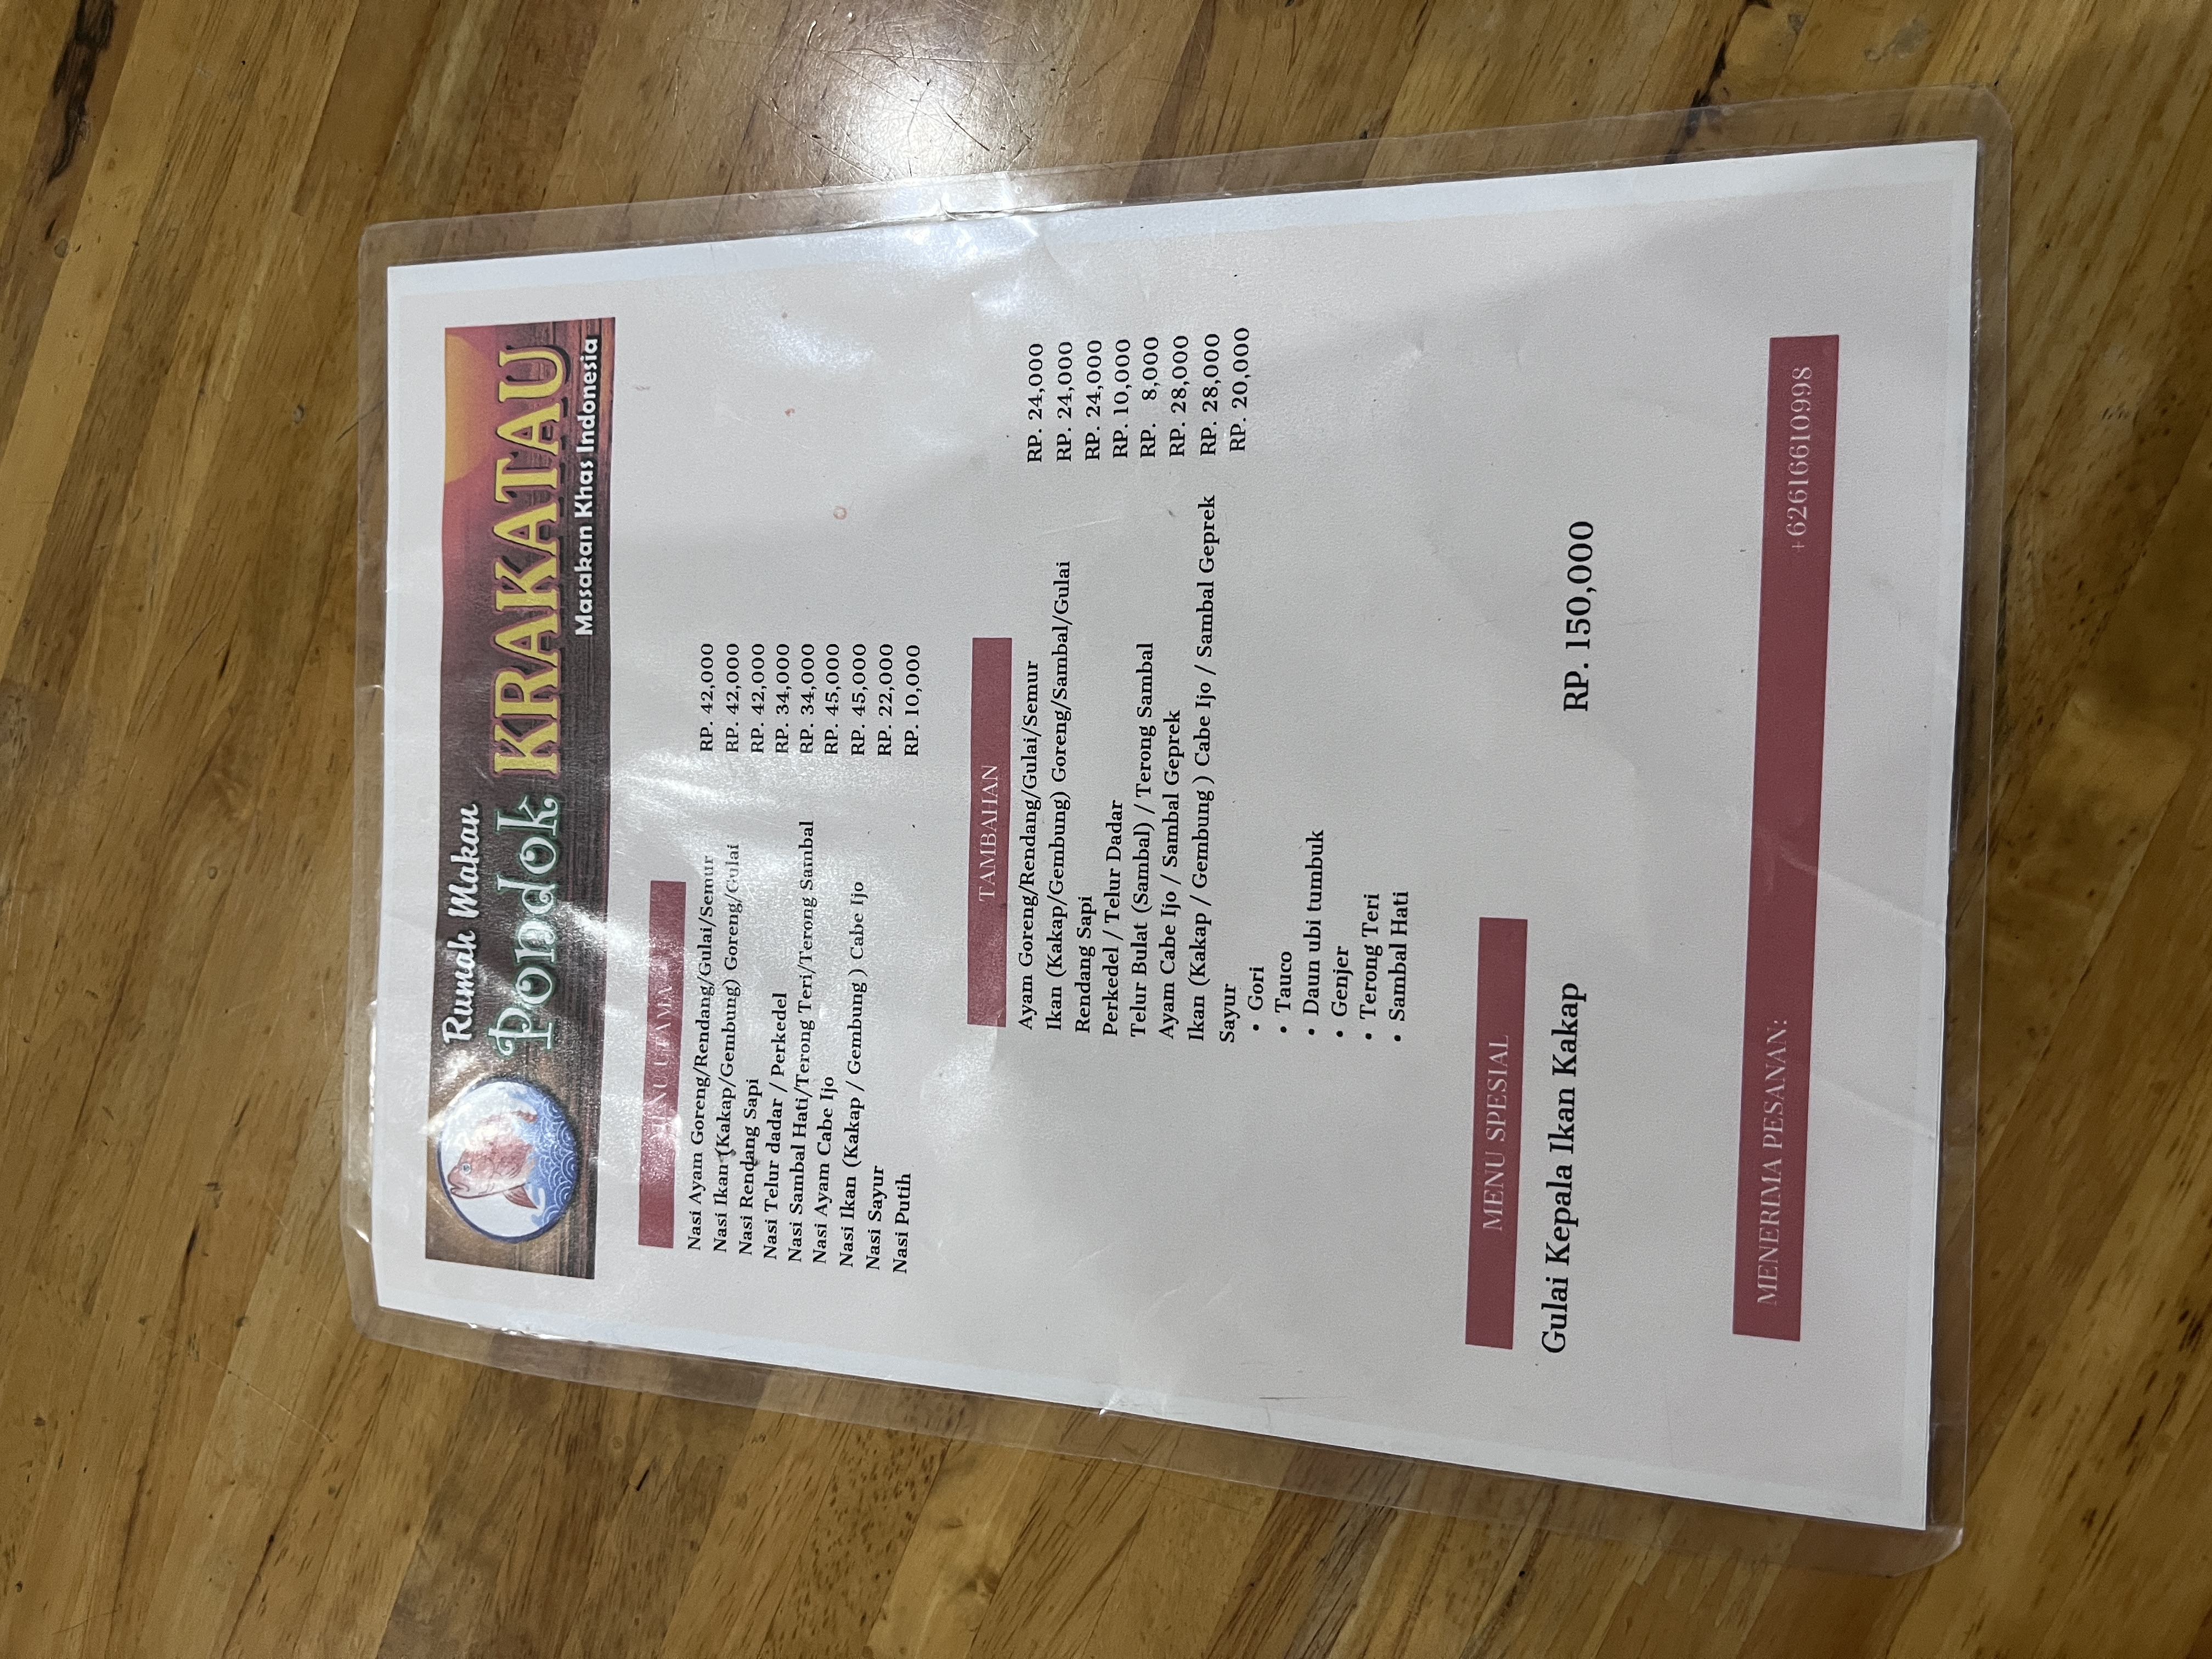
\includegraphics[angle=-90,origin=c,width=\linewidth,height=0.245\textheight,keepaspectratio]{resource/05-fieldwork/01-wawancara/20260701-20260704-wawancara-lapangan/raw/photos/K03-PA-20260703-pondok-krakatau/K03-PA-20260703-foto-01.jpg}
        \par\vspace{2pt}\footnotesize (c) Dokumentasi menu rumah makan
    \end{minipage}\hfill
    \begin{minipage}[t]{0.47\textwidth}
        \centering
        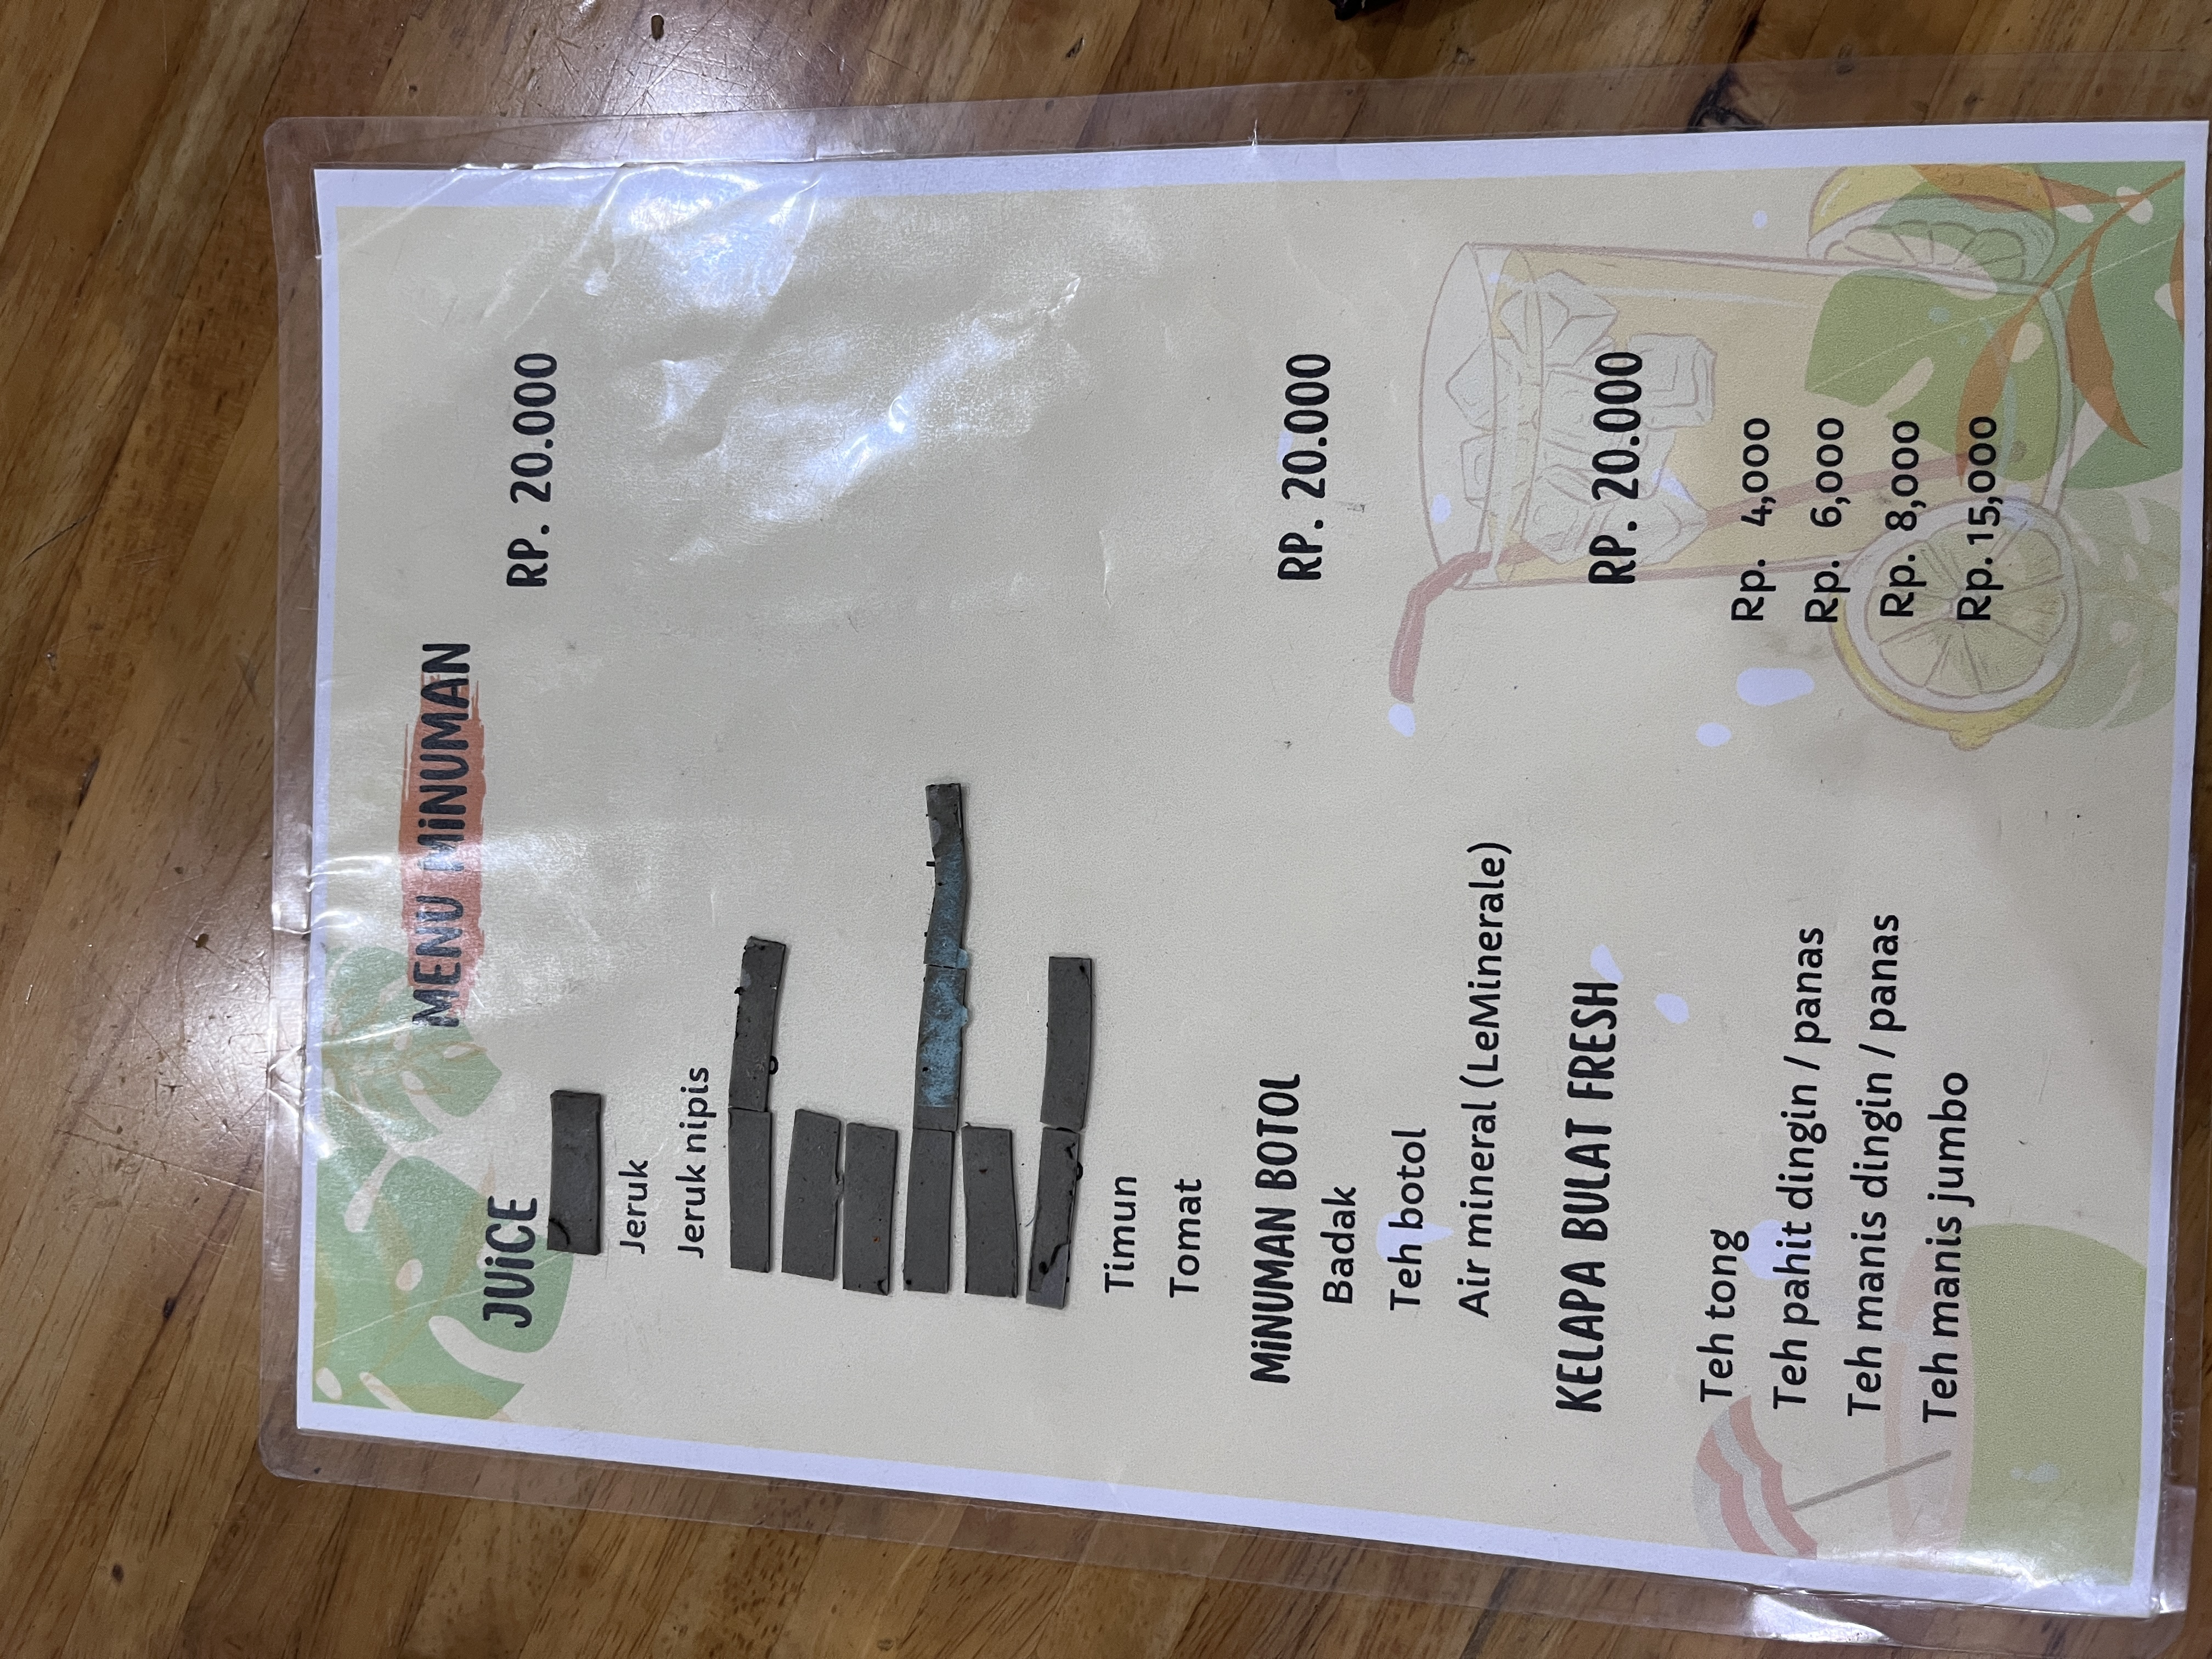
\includegraphics[angle=-90,origin=c,width=\linewidth,height=0.245\textheight,keepaspectratio]{resource/05-fieldwork/01-wawancara/20260701-20260704-wawancara-lapangan/raw/photos/K03-PA-20260703-pondok-krakatau/K03-PA-20260703-foto-02.jpg}
        \par\vspace{2pt}\footnotesize (d) Dokumentasi menu minuman di lokasi
    \end{minipage}
    \figuresource[0.98\textwidth]{Dokumentasi lapangan pada Pondok Krakatau; diolah peneliti (2026).}
    \caption{Dokumentasi Wawancara Kompetitor di Pondok Krakatau}
    \label{fig:dokumentasi-wawancara-pondok-krakatau}
\end{figure}

\FloatBarrier

\lampiransection{DOKUMENTASI KINERJA NASI GERILYA DAN KOMPETITOR PADA GRABFOOD}
\label{app:dokumentasi-indeks-kinerja}

Lampiran ini memuat dokumentasi kinerja untuk penelitian \textit{Analisis Strategi Pemasaran Rumah Makan Nasi Gerilya pada Platform GrabFood Menggunakan Matriks SWOT}. Data yang disajikan mencakup jumlah penjualan bulanan dalam satuan bungkus, indeks \textit{Average Order Value} (AOV), indeks kunjungan harian, dan indeks kompetitor pada platform GrabFood. Jumlah penjualan bulanan disajikan dalam satuan bungkus sesuai grafik penjualan per bulan, sedangkan indeks AOV, indeks kunjungan harian, dan indeks kompetitor disajikan sebagai data turunan untuk membaca arah performa usaha dan posisi pembanding \textit{merchant}.

\begin{table}[!htbp]
    \centering
    \caption{Jumlah Penjualan Bulanan Nasi Gerilya}
    \label{tab:jumlah_penjualan_bungkus_grabfood}
    \begin{tabular}{|l|c|c|}
        \toprule
        \textbf{Periode} & \textbf{Jumlah Penjualan (Bungkus)} & \textbf{Perubahan} \\ \hline
        \midrule
        Des-24           & 6.702                               & --                 \\ \hline
        Jan-25           & 8.740                               & +30,4\%            \\ \hline
        Feb-25           & 8.911                               & +2,0\%             \\ \hline
        Mar-25           & 16.590                              & +86,2\%            \\ \hline
        Apr-25           & 15.129                              & -8,8\%             \\ \hline
        Mei-25           & 14.580                              & -3,6\%             \\ \hline
        Jun-25           & 13.467                              & -7,6\%             \\ \hline
        Jul-25           & 14.633                              & +8,7\%             \\ \hline
        Ags-25           & 14.259                              & -2,6\%             \\ \hline
        Sep-25           & 14.034                              & -1,6\%             \\ \hline
        Okt-25           & 13.009                              & -7,3\%             \\ \hline
        Nov-25           & 12.900                              & -0,8\%             \\ \hline
        \bottomrule
    \end{tabular}
    \tablesource{Dokumentasi grafik penjualan bulanan Nasi Gerilya; diolah peneliti (2026).}
\end{table}

\begin{table}[!t]
    \centering
    \caption{Indeks \textit{Average Order Value} (AOV)}
    \label{tab:indeks_aov_grabfood}
    \begin{tabular}{|l|c|c|}
        \toprule
        \textbf{Periode} & \textbf{Indeks} & \textbf{Perubahan} \\ \hline
        \midrule
        Jul-25           & 100,0           & --                 \\ \hline
        Ags-25           & 102,0           & +2,0\%             \\ \hline
        Sep-25           & 107,9           & +5,8\%             \\ \hline
        Okt-25           & 110,0           & +1,9\%             \\ \hline
        Nov-25           & 114,5           & +4,1\%             \\ \hline
        \bottomrule
    \end{tabular}
    \tablesource{Dokumentasi internal Nasi Gerilya; diolah peneliti (2026).}
\end{table}

\begin{table}[!t]
    \centering
    \caption{Indeks Kunjungan Harian}
    \label{tab:indeks_kunjungan_grabfood}
    \begin{tabular}{|l|c|c|}
        \toprule
        \textbf{Periode} & \textbf{Indeks} & \textbf{Perubahan} \\ \hline
        \midrule
        Sep-25           & 100,0           & --                 \\ \hline
        Okt-25           & 116,5           & +16,5\%            \\ \hline
        Nov-25           & 130,7           & +12,2\%            \\ \hline
        \bottomrule
    \end{tabular}
    \tablesource{Dokumentasi internal Nasi Gerilya; diolah peneliti (2026).}
\end{table}

\begin{table}[!t]
    \centering
    \small
    \caption{Indeks Kompetitor Nasi Padang Juli--Oktober 2025}
    \label{tab:indeks_kompetitor_grabfood}
    \begin{tabularx}{\textwidth}{|Y|>{\centering\arraybackslash}p{1.15cm}|>{\centering\arraybackslash}p{1.15cm}|>{\centering\arraybackslash}p{1.15cm}|>{\centering\arraybackslash}p{1.15cm}|>{\centering\arraybackslash}p{1.75cm}|}
        \toprule
        \textbf{\textit{Merchant}} & \textbf{Jul} & \textbf{Ags} & \textbf{Sep} & \textbf{Okt} & \textbf{\shortstack{$\Delta$ Jul--Okt}} \\ \hline
        \midrule
        Koto Gadang                & 100,0        & 105,1        & 86,2         & 94,2         & -5,8\%                                  \\ \hline
        Pondok Krakatau            & 100,0        & 110,1        & 89,0         & 107,5        & +7,5\%                                  \\ \hline
        Uda Sayang                 & 100,0        & 94,1         & 89,0         & 88,9         & -11,1\%                                 \\ \hline
        Dendeng Batokok            & 100,0        & 104,1        & 85,2         & 95,1         & -4,9\%                                  \\ \hline
        Istana Krakatau            & 100,0        & 119,2        & 108,4        & 119,3        & +19,3\%                                 \\ \hline
        Sederhana                  & 100,0        & 97,5         & 94,9         & 98,6         & -1,4\%                                  \\ \hline
        Gumarang Jaya              & 100,0        & 116,1        & 102,6        & 114,1        & +14,1\%                                 \\ \hline
        Nasi Gerilya               & 100,0        & 92,6         & 87,8         & 70,4         & -29,6\%                                 \\ \hline
        Garuda                     & 100,0        & 95,5         & 90,1         & 93,9         & -6,1\%                                  \\ \hline
        Pondok Gurih               & 100,0        & 102,9        & 97,0         & 101,5        & +1,5\%                                  \\ \hline
        \bottomrule
    \end{tabularx}
    \tablesource{Dokumentasi internal dan pembanding \textit{merchant}; diolah peneliti (2026).}
\end{table}

\FloatBarrier
Data pada Tabel~\ref{tab:jumlah_penjualan_bungkus_grabfood}, \ref{tab:indeks_aov_grabfood}, \ref{tab:indeks_kunjungan_grabfood}, dan \ref{tab:indeks_kompetitor_grabfood} digunakan sebagai dasar pembacaan arah performa usaha dan posisi pembanding pada platform GrabFood.

\lampiransection{Bukti Observasi GrabFood Nasi Gerilya 13 Juni 2026}
\label{app:evidence-observasi-grabfood-20260613}

Lampiran ini memuat bukti visual dari observasi halaman GrabFood Nasi Gerilya - Glugur Kota pada 13 Juni 2026. Bukti visual digunakan untuk memperjelas temuan mengenai profil toko, rating, promo, menu, harga, ketersediaan produk, dan ulasan pelanggan yang dibahas pada Bab IV. Kode data dicantumkan agar hubungan antara bukti visual, ringkasan temuan, dan pembahasan dapat ditelusuri secara jelas.

Bukti visual dalam lampiran ini disajikan bersama keterangan singkat untuk mendukung proses pemeriksaan data dan penarikan temuan penelitian.

\begin{table}[!htbp]
    \centering
    \caption{Identitas Bukti Observasi GrabFood}
    \label{tab:identitas-evidence-observasi-grabfood-20260613}
    \begin{tabularx}{\textwidth}{|Z{3.4cm}|Y|}
        \toprule
        \textbf{Aspek} & \textbf{Keterangan} \\ \hline
        \midrule
        Objek observasi & Nasi Gerilya - Glugur Kota \\ \hline
        Platform & GrabFood \\ \hline
        Tanggal observasi & 13 Juni 2026 \\ \hline
        Fokus bukti & Profil toko, rating, jumlah penilaian, promo/voucher, menu, harga, foto produk, menu tidak tersedia, dan ulasan pelanggan \\ \hline
        Jumlah bukti visual & 76 bukti visual \\ \hline
        \bottomrule
    \end{tabularx}
    \tablesource{Diolah peneliti dari observasi GrabFood Nasi Gerilya tanggal 13 Juni 2026.}
\end{table}

\begin{table}[!htbp]
    \centering
    \caption{Ringkasan Kelompok Bukti Observasi}
    \label{tab:ringkasan-kelompok-evidence-grabfood-20260613}
    \footnotesize
    \setlength{\tabcolsep}{4pt}
    \renewcommand{\arraystretch}{0.95}
    \begin{tabularx}{\textwidth}{|Z{3cm}|c|Y|Y|}
        \toprule
        \textbf{Kelompok Bukti} & \textbf{Jumlah} & \textbf{Isi Data} & \textbf{Kegunaan Analisis} \\ \hline
        \midrule
        Profil dan rating & 4 & Nama toko, kategori, status toko, jarak, rating, jumlah penilaian, dan ringkasan ulasan agregat & Identitas objek, reputasi platform, dan bukti fisik digital \\ \hline
        Promo dan voucher & 19 & Promo persentase, potongan nominal, diskon ongkir, bank, dan \textit{group order} & Analisis promosi, insentif harga, dan peluang platform \\ \hline
        Menu, harga, dan foto & 24 & Menu utama, menu terlaris, menu promo, minuman, sambal, tambahan, harga, dan foto produk & Analisis produk, harga, variasi menu, dan tampilan digital \\ \hline
        Menu tidak tersedia & 6 & Menu atau produk yang terlihat berstatus \textit{Nggak tersedia} & Analisis ketersediaan stok, proses operasional, dan risiko pengalaman pelanggan \\ \hline
        Ringkasan harga & 3 & Rentang harga keseluruhan, rentang harga item tersedia, dan harga menu utama tersedia & Analisis harga dan pembeda harga aktif dibanding item tidak tersedia \\ \hline
        Ulasan positif & 10 & Ulasan pelanggan positif mengenai rasa, porsi, kesegaran, kebersihan, request, kemasan, dan pembelian rutin & Dasar identifikasi kekuatan internal dan loyalitas pelanggan \\ \hline
        Ulasan negatif/netral & 10 & Ulasan mengenai salah item, item kurang lengkap, add-on tidak diberikan, harga/porsi, kualitas, koordinasi staf, dan pengalaman pascakonsumsi & Dasar identifikasi kelemahan, risiko layanan, dan kebutuhan triangulasi \\ \hline
        \bottomrule
    \end{tabularx}
    \tablesource{Diolah peneliti dari observasi GrabFood tanggal 13 Juni 2026.}
\end{table}

\begin{table}[!htbp]
    \centering
    \caption{Pemetaan Kode Temuan dan Kode Data Pendukung Observasi GrabFood}
    \label{tab:temuan-utama-evidence-observasi-grabfood-20260613}
    \scriptsize
    \setlength{\tabcolsep}{3pt}
    \renewcommand{\arraystretch}{0.95}
    \begin{tabularx}{\textwidth}{|Z{1.55cm}|Z{2.45cm}|Y|Y|}
        \toprule
        \textbf{Kode Temuan} & \textbf{Temuan} & \textbf{Keterangan} & \textbf{Kode Data Pendukung} \\ \hline
        \midrule
        TO-GF-01 & Identitas dan reputasi toko & Nama toko, status toko, jarak, dan rating 4,7 dari 4.584 penilaian terlihat pada halaman GrabFood Nasi Gerilya. & GF-PROFILE-001; GF-PROFILE-002; GF-RATING-001 \\ \hline
        TO-GF-02 & Ringkasan ulasan agregat & Ringkasan ulasan agregat menyebut rasa enak, porsi besar, bahan segar, kemasan rapi, menu beragam, dan harga terjangkau. & GF-REVIEW-SUMMARY-001 \\ \hline
        TO-GF-03 & Promo aktif & Terdapat 19 promo/voucher yang terlihat pada halaman Promo GrabFood, termasuk diskon persentase, potongan nominal, diskon ongkir, bank, dan \textit{group order}. & GF-PROMO-001--GF-PROMO-019 \\ \hline
        TO-GF-04 & Menu terlaris & Menu berlabel terlaris yang terlihat adalah Nasi Padang Rendang Sapi, Nasi Padang Ayam Goreng Bumbu, dan Nasi Padang Ayam Rendang. & GF-MENU-TERLARIS-001--GF-MENU-TERLARIS-003 \\ \hline
        TO-GF-05 & Rentang harga aktif & Rentang harga item tersedia yang dikodekan adalah Rp1.100--Rp72.000, sedangkan paket nasi Padang tersedia berada pada Rp27.500--Rp72.000. & GF-PRICE-RANGE-001; GF-PRICE-RANGE-003 \\ \hline
        TO-GF-06 & Menu tidak tersedia & Terdapat 6 menu atau produk yang terlihat berstatus \textit{Nggak tersedia}, termasuk menu premium kepala ikan dan produk sambal kemasan. & GF-SOLDOUT-001--GF-SOLDOUT-006 \\ \hline
        TO-GF-07 & Tema ulasan positif & Pelanggan menonjolkan rasa, porsi, kesegaran bahan, kebersihan, pengemasan, request yang dipenuhi, dan kebiasaan membeli ulang. & GF-REV-POS-001--GF-REV-POS-010 \\ \hline
        TO-GF-08 & Tema ulasan negatif/netral & Keluhan berkaitan dengan salah item, item kurang lengkap, add-on tidak diberikan, persepsi harga/porsi, kesegaran, koordinasi staf, dan risiko pengalaman pascakonsumsi. & GF-REV-NEG-001--GF-REV-NEG-010 \\ \hline
        \bottomrule
    \end{tabularx}
    \tablesource{Diolah peneliti dari observasi GrabFood tanggal 13 Juni 2026.}
\end{table}

\clearpage
\subsection*{Bukti Visual Observasi GrabFood}

Bukti visual berikut disajikan sebagai pendukung temuan observasi GrabFood. Keterangan pada caption gambar menunjukkan kode data dan data utama yang digunakan pada ringkasan dan pembahasan Bab IV.

\newlength{\gfEvidenceMaxHeight}
\newcommand{\gfEvidenceBlock}[4]{%
    \setlength{\gfEvidenceMaxHeight}{#4\textheight}%
    \setlength{\gfEvidenceMaxHeight}{0.7\gfEvidenceMaxHeight}%
    \par\noindent\begin{minipage}{\textwidth}%
        \centering
        \includegraphics[width=0.62\textwidth,height=\gfEvidenceMaxHeight,keepaspectratio]{#3}\par
        \figuresource[0.62\textwidth]{Dokumentasi observasi GrabFood Nasi Gerilya tanggal 13 Juni 2026; diolah peneliti (2026).}
        \captionof{figure}{#1 -- #2}%
    \end{minipage}\par\vspace{7pt}%
}

\newcommand{\gfEvidenceCompactBlock}[4]{%
    \setlength{\gfEvidenceMaxHeight}{#4\textheight}%
    \setlength{\gfEvidenceMaxHeight}{0.58\gfEvidenceMaxHeight}%
    \par\noindent\begin{minipage}{\textwidth}%
        \centering
        \includegraphics[width=0.56\textwidth,height=\gfEvidenceMaxHeight,keepaspectratio]{#3}\par
        \figuresource[0.56\textwidth]{Dokumentasi observasi GrabFood Nasi Gerilya tanggal 13 Juni 2026; diolah peneliti (2026).}
        \captionof{figure}{#1 -- #2}%
    \end{minipage}\par\vspace{4pt}%
}

% File ini digenerate dari O-GF-20260613-coded-manifest.csv.
% Jangan edit manual jika manifest berubah; regenerate dari manifest.
\subsection*{Profil dan Rating}

\gfEvidenceBlock{GF-PROFILE-001}{Nasi Gerilya - Glugur Kota}{resource/05-fieldwork/02-observasi-grabfood/20260613-nasi-gerilya/coded-data/profile-rating/gf-profile-001-nasi-gerilya-glugur-kota.jpeg}{0.26}

\gfEvidenceBlock{GF-PROFILE-002}{Tutup; buka besok; jarak 6.6 km; badge Grab bintang 5 dan centang}{resource/05-fieldwork/02-observasi-grabfood/20260613-nasi-gerilya/coded-data/profile-rating/gf-profile-002-tutup-buka-besok-jarak-6-6-km-badge-grab-bintang-5-dan-centang.jpeg}{0.26}

\gfEvidenceBlock{GF-RATING-001}{Rating 4.7 dari 4.584 penilaian}{resource/05-fieldwork/02-observasi-grabfood/20260613-nasi-gerilya/coded-data/profile-rating/gf-rating-001-rating-4-7-dari-4-584-penilaian.jpeg}{0.26}

\gfEvidenceBlock{GF-REVIEW-SUMMARY-001}{AI summary: rasa enak, porsi besar, bahan segar, kemasan rapi, menu beragam, harga terjangkau}{resource/05-fieldwork/02-observasi-grabfood/20260613-nasi-gerilya/coded-data/profile-rating/gf-review-summary-001-ai-summary-rasa-enak-porsi-besar-bahan-segar-kemasan-rapi-menu-berag.jpeg}{0.40}

\clearpage
\subsection*{Promo dan Voucher}

\gfEvidenceBlock{GF-PROMO-001}{Diskon 17\% hingga Rp50.000; tanpa belanja minimum}{resource/05-fieldwork/02-observasi-grabfood/20260613-nasi-gerilya/coded-data/promo-voucher/gf-promo-001-diskon-17-hingga-rp50-000-tanpa-belanja-minimum.jpeg}{0.26}

\gfEvidenceBlock{GF-PROMO-002}{Diskon Rp15.000 BSI; minimum belanja terlihat terpotong}{resource/05-fieldwork/02-observasi-grabfood/20260613-nasi-gerilya/coded-data/promo-voucher/gf-promo-002-diskon-rp15-000-bsi-minimum-belanja-terlihat-terpotong.jpeg}{0.26}

\gfEvidenceBlock{GF-PROMO-003}{Diskon Rp10.000 BTN; minimum belanja terlihat terpotong}{resource/05-fieldwork/02-observasi-grabfood/20260613-nasi-gerilya/coded-data/promo-voucher/gf-promo-003-diskon-rp10-000-btn-minimum-belanja-terlihat-terpotong.jpeg}{0.26}

\gfEvidenceBlock{GF-PROMO-004}{Diskon Rp25.000 Bank Mega Syariah; minimum belanja terlihat terpotong}{resource/05-fieldwork/02-observasi-grabfood/20260613-nasi-gerilya/coded-data/promo-voucher/gf-promo-004-diskon-rp25-000-bank-mega-syariah-minimum-belanja-terlihat-terpotong.jpeg}{0.26}

\gfEvidenceBlock{GF-PROMO-005}{Diskon Rp4.500 untuk Gulai Cincang Gerilya}{resource/05-fieldwork/02-observasi-grabfood/20260613-nasi-gerilya/coded-data/promo-voucher/gf-promo-005-diskon-rp4-500-untuk-gulai-cincang-gerilya.jpeg}{0.26}

\gfEvidenceBlock{GF-PROMO-006}{Diskon Rp15.000 Bank Mega; minimum belanja terlihat terpotong}{resource/05-fieldwork/02-observasi-grabfood/20260613-nasi-gerilya/coded-data/promo-voucher/gf-promo-006-diskon-rp15-000-bank-mega-minimum-belanja-terlihat-terpotong.jpeg}{0.26}

\gfEvidenceBlock{GF-PROMO-007}{Diskon Rp25.000 Bank Mega; minimum belanja terlihat terpotong}{resource/05-fieldwork/02-observasi-grabfood/20260613-nasi-gerilya/coded-data/promo-voucher/gf-promo-007-diskon-rp25-000-bank-mega-minimum-belanja-terlihat-terpotong.jpeg}{0.26}

\gfEvidenceBlock{GF-PROMO-008}{Diskon 5\% untuk Group Order; minimum orang bergabung 3 ke 6}{resource/05-fieldwork/02-observasi-grabfood/20260613-nasi-gerilya/coded-data/promo-voucher/gf-promo-008-diskon-5-untuk-group-order-minimum-orang-bergabung-3-ke-6.jpeg}{0.26}

\gfEvidenceBlock{GF-PROMO-009}{Diskon Rp4.000 Bank Mega; minimum belanja terlihat terpotong}{resource/05-fieldwork/02-observasi-grabfood/20260613-nasi-gerilya/coded-data/promo-voucher/gf-promo-009-diskon-rp4-000-bank-mega-minimum-belanja-terlihat-terpotong.jpeg}{0.26}

\gfEvidenceBlock{GF-PROMO-010}{Diskon Rp10.000 Bank Mega; minimum belanja terlihat terpotong}{resource/05-fieldwork/02-observasi-grabfood/20260613-nasi-gerilya/coded-data/promo-voucher/gf-promo-010-diskon-rp10-000-bank-mega-minimum-belanja-terlihat-terpotong.jpeg}{0.26}

\gfEvidenceBlock{GF-PROMO-011}{Diskon ongkir Rp3.000; tanpa belanja minimum}{resource/05-fieldwork/02-observasi-grabfood/20260613-nasi-gerilya/coded-data/promo-voucher/gf-promo-011-diskon-ongkir-rp3-000-tanpa-belanja-minimum.jpeg}{0.26}

\gfEvidenceBlock{GF-PROMO-012}{Diskon Rp25.000 BSI; minimum belanja terlihat terpotong}{resource/05-fieldwork/02-observasi-grabfood/20260613-nasi-gerilya/coded-data/promo-voucher/gf-promo-012-diskon-rp25-000-bsi-minimum-belanja-terlihat-terpotong.jpeg}{0.26}

\gfEvidenceBlock{GF-PROMO-013}{Diskon Rp25.000 Raya Bank; minimum belanja terlihat terpotong}{resource/05-fieldwork/02-observasi-grabfood/20260613-nasi-gerilya/coded-data/promo-voucher/gf-promo-013-diskon-rp25-000-raya-bank-minimum-belanja-terlihat-terpotong.jpeg}{0.26}

\gfEvidenceBlock{GF-PROMO-014}{Diskon 25\% s.d. Rp100.000; minimum belanja Rp30.000}{resource/05-fieldwork/02-observasi-grabfood/20260613-nasi-gerilya/coded-data/promo-voucher/gf-promo-014-diskon-25-s-d-rp100-000-minimum-belanja-rp30-000.jpeg}{0.26}

\gfEvidenceBlock{GF-PROMO-015}{Diskon Rp15.000 BTN; minimum belanja terlihat terpotong}{resource/05-fieldwork/02-observasi-grabfood/20260613-nasi-gerilya/coded-data/promo-voucher/gf-promo-015-diskon-rp15-000-btn-minimum-belanja-terlihat-terpotong.jpeg}{0.26}

\gfEvidenceBlock{GF-PROMO-016}{Diskon ongkir Rp8.000; minimum belanja terlihat terpotong}{resource/05-fieldwork/02-observasi-grabfood/20260613-nasi-gerilya/coded-data/promo-voucher/gf-promo-016-diskon-ongkir-rp8-000-minimum-belanja-terlihat-terpotong.jpeg}{0.26}

\gfEvidenceBlock{GF-PROMO-017}{Diskon ongkir Rp8.000; minimum belanja terlihat terpotong}{resource/05-fieldwork/02-observasi-grabfood/20260613-nasi-gerilya/coded-data/promo-voucher/gf-promo-017-diskon-ongkir-rp8-000-minimum-belanja-terlihat-terpotong.jpeg}{0.26}

\gfEvidenceBlock{GF-PROMO-018}{Diskon Rp20.000 SBI card; minimum belanja terlihat terpotong}{resource/05-fieldwork/02-observasi-grabfood/20260613-nasi-gerilya/coded-data/promo-voucher/gf-promo-018-diskon-rp20-000-sbi-card-minimum-belanja-terlihat-terpotong.jpeg}{0.26}

\gfEvidenceBlock{GF-PROMO-019}{Diskon Rp20.000 Bank Jakarta; minimum belanja terlihat terpotong}{resource/05-fieldwork/02-observasi-grabfood/20260613-nasi-gerilya/coded-data/promo-voucher/gf-promo-019-diskon-rp20-000-bank-jakarta-minimum-belanja-terlihat-terpotong.jpeg}{0.26}

\clearpage
\subsection*{Menu, Harga, dan Foto Produk}

\gfEvidenceBlock{GF-MENU-TERATAS-001}{Nasi Padang Bungkus Gulai Cincang; Rp50.500 dari Rp55.000}{resource/05-fieldwork/02-observasi-grabfood/20260613-nasi-gerilya/coded-data/menu-harga-foto/gf-menu-teratas-001-nasi-padang-bungkus-gulai-cincang-rp50-500-dari-rp55-000.jpeg}{0.26}

\gfEvidenceBlock{GF-MENU-TERATAS-002}{Nasi Padang Kari Kambing GERILYA; Rp72.000}{resource/05-fieldwork/02-observasi-grabfood/20260613-nasi-gerilya/coded-data/menu-harga-foto/gf-menu-teratas-002-nasi-padang-kari-kambing-gerilya-rp72-000.jpeg}{0.26}

\gfEvidenceBlock{GF-MENU-TERATAS-003}{Nasi Padang Dendeng Sapi Bakar GERILYA; Rp56.000}{resource/05-fieldwork/02-observasi-grabfood/20260613-nasi-gerilya/coded-data/menu-harga-foto/gf-menu-teratas-003-nasi-padang-dendeng-sapi-bakar-gerilya-rp56-000.jpeg}{0.26}

\gfEvidenceBlock{GF-MENU-TERLARIS-001}{Nasi Padang Rendang Sapi GERILYA; Rp56.000; label Terlaris}{resource/05-fieldwork/02-observasi-grabfood/20260613-nasi-gerilya/coded-data/menu-harga-foto/gf-menu-terlaris-001-nasi-padang-rendang-sapi-gerilya-rp56-000-label-terlaris.jpeg}{0.26}

\gfEvidenceBlock{GF-MENU-TERLARIS-002}{Nasi Padang Ayam Goreng Bumbu GERILYA; Rp45.000; label Terlaris}{resource/05-fieldwork/02-observasi-grabfood/20260613-nasi-gerilya/coded-data/menu-harga-foto/gf-menu-terlaris-002-nasi-padang-ayam-goreng-bumbu-gerilya-rp45-000-label-terlaris.jpeg}{0.26}

\gfEvidenceBlock{GF-MENU-TERLARIS-003}{Nasi Padang Ayam Rendang GERILYA; Rp46.000; label Terlaris}{resource/05-fieldwork/02-observasi-grabfood/20260613-nasi-gerilya/coded-data/menu-harga-foto/gf-menu-terlaris-003-nasi-padang-ayam-rendang-gerilya-rp46-000-label-terlaris.jpeg}{0.26}

\gfEvidenceBlock{GF-MENU-PROMO-002}{Nasi Padang Gulai Ayam Kalasan GERILYA; Rp41.500 dari Rp46.000}{resource/05-fieldwork/02-observasi-grabfood/20260613-nasi-gerilya/coded-data/menu-harga-foto/gf-menu-promo-002-nasi-padang-gulai-ayam-kalasan-gerilya-rp41-500-dari-rp46-000.jpeg}{0.26}

\gfEvidenceBlock{GF-MENU-UTAMA-001}{Nasi Padang Ayam Bakar GERILYA; Rp45.000}{resource/05-fieldwork/02-observasi-grabfood/20260613-nasi-gerilya/coded-data/menu-harga-foto/gf-menu-utama-001-nasi-padang-ayam-bakar-gerilya-rp45-000.jpeg}{0.26}

\gfEvidenceBlock{GF-MENU-UTAMA-002}{Nasi Padang Cumi Nagih GERILYA; Rp70.000}{resource/05-fieldwork/02-observasi-grabfood/20260613-nasi-gerilya/coded-data/menu-harga-foto/gf-menu-utama-002-nasi-padang-cumi-nagih-gerilya-rp70-000.jpeg}{0.26}

\gfEvidenceBlock{GF-MENU-UTAMA-003}{Nasi Padang Ikan Lele Goreng Panas GERILYA; Rp39.000}{resource/05-fieldwork/02-observasi-grabfood/20260613-nasi-gerilya/coded-data/menu-harga-foto/gf-menu-utama-003-nasi-padang-ikan-lele-goreng-panas-gerilya-rp39-000.jpeg}{0.26}

\gfEvidenceBlock{GF-MENU-UTAMA-004}{Nasi Padang Ikan Tongkol Tuna Goreng Panas GERILYA; Rp48.000}{resource/05-fieldwork/02-observasi-grabfood/20260613-nasi-gerilya/coded-data/menu-harga-foto/gf-menu-utama-004-nasi-padang-ikan-tongkol-tuna-goreng-panas-gerilya-rp48-000.jpeg}{0.26}

\gfEvidenceBlock{GF-MENU-UTAMA-005}{Nasi Padang Ikan Gembung Goreng GERILYA; Rp50.000}{resource/05-fieldwork/02-observasi-grabfood/20260613-nasi-gerilya/coded-data/menu-harga-foto/gf-menu-utama-005-nasi-padang-ikan-gembung-goreng-gerilya-rp50-000.jpeg}{0.26}

\gfEvidenceBlock{GF-MENU-UTAMA-006}{Nasi Padang Ikan Nila Goreng GERILYA; Rp43.000}{resource/05-fieldwork/02-observasi-grabfood/20260613-nasi-gerilya/coded-data/menu-harga-foto/gf-menu-utama-006-nasi-padang-ikan-nila-goreng-gerilya-rp43-000.jpeg}{0.26}

\gfEvidenceBlock{GF-MENU-UTAMA-007}{Nasi Padang Telur Dadar GERILYA; Rp32.000}{resource/05-fieldwork/02-observasi-grabfood/20260613-nasi-gerilya/coded-data/menu-harga-foto/gf-menu-utama-007-nasi-padang-telur-dadar-gerilya-rp32-000.jpeg}{0.26}

\gfEvidenceBlock{GF-MENU-UTAMA-008}{Nasi Padang Berkedel Kentang GERILYA; Rp37.400}{resource/05-fieldwork/02-observasi-grabfood/20260613-nasi-gerilya/coded-data/menu-harga-foto/gf-menu-utama-008-nasi-padang-berkedel-kentang-gerilya-rp37-400.jpeg}{0.26}

\gfEvidenceBlock{GF-MENU-UTAMA-009}{Nasi Padang Sayur Polos GERILYA; Rp27.500}{resource/05-fieldwork/02-observasi-grabfood/20260613-nasi-gerilya/coded-data/menu-harga-foto/gf-menu-utama-009-nasi-padang-sayur-polos-gerilya-rp27-500.jpeg}{0.26}

\gfEvidenceBlock{GF-MENU-MINUMAN-001}{Air Mineral 400ml; Rp13.200}{resource/05-fieldwork/02-observasi-grabfood/20260613-nasi-gerilya/coded-data/menu-harga-foto/gf-menu-minuman-001-air-mineral-400ml-rp13-200.jpeg}{0.26}

\gfEvidenceBlock{GF-MENU-MINUMAN-002}{Es Teh Tawar; Rp13.200}{resource/05-fieldwork/02-observasi-grabfood/20260613-nasi-gerilya/coded-data/menu-harga-foto/gf-menu-minuman-002-es-teh-tawar-rp13-200.jpeg}{0.26}

\gfEvidenceBlock{GF-MENU-MINUMAN-003}{Es Teh Manis; Rp15.950}{resource/05-fieldwork/02-observasi-grabfood/20260613-nasi-gerilya/coded-data/menu-harga-foto/gf-menu-minuman-003-es-teh-manis-rp15-950.jpeg}{0.26}

\gfEvidenceBlock{GF-MENU-MINUMAN-004}{Es Jeruk Limau; Rp22.000}{resource/05-fieldwork/02-observasi-grabfood/20260613-nasi-gerilya/coded-data/menu-harga-foto/gf-menu-minuman-004-es-jeruk-limau-rp22-000.jpeg}{0.26}

\gfEvidenceBlock{GF-MENU-TAMBAHAN-001}{Nambah KUAH CAMPUR; Rp2.500}{resource/05-fieldwork/02-observasi-grabfood/20260613-nasi-gerilya/coded-data/menu-harga-foto/gf-menu-tambahan-001-nambah-kuah-campur-rp2-500.jpeg}{0.26}

\gfEvidenceBlock{GF-MENU-TAMBAHAN-002}{Nambah Kuah Gulai Kuning; Rp1.100}{resource/05-fieldwork/02-observasi-grabfood/20260613-nasi-gerilya/coded-data/menu-harga-foto/gf-menu-tambahan-002-nambah-kuah-gulai-kuning-rp1-100.jpeg}{0.26}

\gfEvidenceBlock{GF-MENU-SAMBAL-001}{GERILYA Sambal Hijau; Rp17.500}{resource/05-fieldwork/02-observasi-grabfood/20260613-nasi-gerilya/coded-data/menu-harga-foto/gf-menu-sambal-001-gerilya-sambal-hijau-rp17-500.jpeg}{0.26}

\gfEvidenceBlock{GF-MENU-SAMBAL-002}{GERILYA Sambal Andaliman Getir Kemasan; Rp38.500}{resource/05-fieldwork/02-observasi-grabfood/20260613-nasi-gerilya/coded-data/menu-harga-foto/gf-menu-sambal-002-gerilya-sambal-andaliman-getir-kemasan-rp38-500.jpeg}{0.26}

\clearpage
\subsection*{Menu Tidak Tersedia}

\gfEvidenceBlock{GF-SOLDOUT-001}{Gulai Merah Kepala Ikan GERILYA L; Rp275.000; Nggak tersedia}{resource/05-fieldwork/02-observasi-grabfood/20260613-nasi-gerilya/coded-data/sold-out/gf-soldout-001-gulai-merah-kepala-ikan-gerilya-l-rp275-000-nggak-tersedia.jpeg}{0.32}

\gfEvidenceBlock{GF-SOLDOUT-002}{Gulai Merah Kepala Ikan GERILYA M; Rp248.050; Nggak tersedia}{resource/05-fieldwork/02-observasi-grabfood/20260613-nasi-gerilya/coded-data/sold-out/gf-soldout-002-gulai-merah-kepala-ikan-gerilya-m-rp248-050-nggak-tersedia.jpeg}{0.26}

\gfEvidenceBlock{GF-SOLDOUT-003}{Nasi Padang Gembung Kuring Bakar GERILYA; Rp47.850; Nggak tersedia}{resource/05-fieldwork/02-observasi-grabfood/20260613-nasi-gerilya/coded-data/sold-out/gf-soldout-003-nasi-padang-gembung-kuring-bakar-gerilya-rp47-850-nggak-tersedia.jpeg}{0.26}

\gfEvidenceBlock{GF-SOLDOUT-004}{Nasi Padang Ayam Pop Sauce Creamy GERILYA; Rp46.000; Nggak tersedia}{resource/05-fieldwork/02-observasi-grabfood/20260613-nasi-gerilya/coded-data/sold-out/gf-soldout-004-nasi-padang-ayam-pop-sauce-creamy-gerilya-rp46-000-nggak-tersedia.jpeg}{0.26}

\gfEvidenceBlock{GF-SOLDOUT-005}{GERILYA Sambal Cumi Nagih Kemasan; Rp38.500; Nggak tersedia}{resource/05-fieldwork/02-observasi-grabfood/20260613-nasi-gerilya/coded-data/sold-out/gf-soldout-005-gerilya-sambal-cumi-nagih-kemasan-rp38-500-nggak-tersedia.jpeg}{0.26}

\gfEvidenceBlock{GF-SOLDOUT-006}{GERILYA Sambal Tuna Asap Keumamah Aceh Kemasan; Rp38.500; Nggak tersedia}{resource/05-fieldwork/02-observasi-grabfood/20260613-nasi-gerilya/coded-data/sold-out/gf-soldout-006-gerilya-sambal-tuna-asap-keumamah-aceh-kemasan-rp38-500-nggak-tersedia.jpeg}{0.26}

\clearpage
\subsection*{Ringkasan Harga}

\gfEvidenceBlock{GF-PRICE-RANGE-001}{Rentang harga observasi: Rp1.100 sampai Rp275.000; tersedia: Rp1.100 sampai Rp72.000; paket nasi padang tersedia: Rp27.500 sampai Rp72.000}{resource/05-fieldwork/02-observasi-grabfood/20260613-nasi-gerilya/coded-data/ringkasan-harga/gf-price-range-001-rentang-harga-observasi-rp1-100-sampai-rp275-000-tersedia-rp1-100-sampa.jpeg}{0.40}

\gfEvidenceBlock{GF-PRICE-RANGE-002}{Harga tertinggi terlihat: Gulai Merah Kepala Ikan L Rp275.000 dan M Rp248.050, tetapi tidak tersedia}{resource/05-fieldwork/02-observasi-grabfood/20260613-nasi-gerilya/coded-data/ringkasan-harga/gf-price-range-002-harga-tertinggi-terlihat-gulai-merah-kepala-ikan-l-rp275-000-dan-m-rp24.jpeg}{0.40}

\gfEvidenceBlock{GF-PRICE-RANGE-003}{Harga atas menu utama tersedia: Kari Kambing Rp72.000 dan Dendeng Sapi Bakar Rp56.000}{resource/05-fieldwork/02-observasi-grabfood/20260613-nasi-gerilya/coded-data/ringkasan-harga/gf-price-range-003-harga-atas-menu-utama-tersedia-kari-kambing-rp72-000-dan-dendeng-sapi-b.jpeg}{0.40}

\clearpage
\subsection*{Ulasan Positif}

\gfEvidenceBlock{GF-REV-POS-001}{Muslim M.: keren ni, konsisten rasa}{resource/05-fieldwork/02-observasi-grabfood/20260613-nasi-gerilya/coded-data/ulasan-positif/gf-rev-pos-001-muslim-m-keren-ni-konsisten-rasa.jpeg}{0.32}

\gfEvidenceBlock{GF-REV-POS-002}{Raymond: Ayam popnya wenak dan creamy}{resource/05-fieldwork/02-observasi-grabfood/20260613-nasi-gerilya/coded-data/ulasan-positif/gf-rev-pos-002-raymond-ayam-popnya-wenak-dan-creamy.jpeg}{0.32}

\gfEvidenceBlock{GF-REV-POS-003}{tasyaa: rasanya enak, sayur fresh, porsi agak kebanyakan}{resource/05-fieldwork/02-observasi-grabfood/20260613-nasi-gerilya/coded-data/ulasan-positif/gf-rev-pos-003-tasyaa-rasanya-enak-sayur-fresh-porsi-agak-kebanyakan.jpeg}{0.50}

\gfEvidenceBlock{GF-REV-POS-004}{Wie W.: langganan keluarga; rasa enak, porsi besar, bersih, request dipenuhi}{resource/05-fieldwork/02-observasi-grabfood/20260613-nasi-gerilya/coded-data/ulasan-positif/gf-rev-pos-004-wie-w-langganan-keluarga-rasa-enak-porsi-besar-bersih-request-dipenuhi.jpeg}{0.40}

\gfEvidenceBlock{GF-REV-POS-005}{Wie W.: langgananku setiap Minggu, Best}{resource/05-fieldwork/02-observasi-grabfood/20260613-nasi-gerilya/coded-data/ulasan-positif/gf-rev-pos-005-wie-w-langgananku-setiap-minggu-best.jpeg}{0.32}

\gfEvidenceBlock{GF-REV-POS-006}{ita: ikan gembung dan lele fresh; rasanya enak}{resource/05-fieldwork/02-observasi-grabfood/20260613-nasi-gerilya/coded-data/ulasan-positif/gf-rev-pos-006-ita-ikan-gembung-dan-lele-fresh-rasanya-enak.jpeg}{0.32}

\gfEvidenceBlock{GF-REV-POS-007}{Lina: semua menu enak, semua recommended}{resource/05-fieldwork/02-observasi-grabfood/20260613-nasi-gerilya/coded-data/ulasan-positif/gf-rev-pos-007-lina-semua-menu-enak-semua-recommended.jpeg}{0.32}

\gfEvidenceBlock{GF-REV-POS-008}{Gusti: best karena sayur dan lauk dipisah}{resource/05-fieldwork/02-observasi-grabfood/20260613-nasi-gerilya/coded-data/ulasan-positif/gf-rev-pos-008-gusti-best-karena-sayur-dan-lauk-dipisah.jpeg}{0.32}

\gfEvidenceBlock{GF-REV-POS-009}{Derrick: rasanya enak, porsinya besar}{resource/05-fieldwork/02-observasi-grabfood/20260613-nasi-gerilya/coded-data/ulasan-positif/gf-rev-pos-009-derrick-rasanya-enak-porsinya-besar.jpeg}{0.32}

\gfEvidenceBlock{GF-REV-POS-010}{Suba: enak banget menurut keluarga}{resource/05-fieldwork/02-observasi-grabfood/20260613-nasi-gerilya/coded-data/ulasan-positif/gf-rev-pos-010-suba-enak-banget-menurut-keluarga.jpeg}{0.32}

\clearpage
\subsection*{Ulasan Negatif/Netral}

\gfEvidenceCompactBlock{GF-REV-NEG-001}{albert p.: Jangek siram tidak dikasih; restoran meminta maaf dan berjanji memperhatikan kelengkapan}{resource/05-fieldwork/02-observasi-grabfood/20260613-nasi-gerilya/coded-data/ulasan-negatif-netral/gf-rev-neg-001-albert-p-jangek-siram-tidak-dikasih-restoran-meminta-maaf-dan-berjanji-memp.jpeg}{0.62}

\gfEvidenceCompactBlock{GF-REV-NEG-002}{Talia: pesan ayam rendang, dikirim ayam goreng}{resource/05-fieldwork/02-observasi-grabfood/20260613-nasi-gerilya/coded-data/ulasan-negatif-netral/gf-rev-neg-002-talia-pesan-ayam-rendang-dikirim-ayam-goreng.jpeg}{0.32}

\gfEvidenceCompactBlock{GF-REV-NEG-003}{irawaty: udang goreng hanya 3 biji, terlalu mahal, tidak worth it}{resource/05-fieldwork/02-observasi-grabfood/20260613-nasi-gerilya/coded-data/ulasan-negatif-netral/gf-rev-neg-003-irawaty-udang-goreng-hanya-3-biji-terlalu-mahal-tidak-worth-it.jpeg}{0.32}

\gfEvidenceCompactBlock{GF-REV-NEG-004}{Hendra: pesan ikan kakap tetapi diberikan ikan nila; restoran meminta maaf}{resource/05-fieldwork/02-observasi-grabfood/20260613-nasi-gerilya/coded-data/ulasan-negatif-netral/gf-rev-neg-004-hendra-pesan-ikan-kakap-tetapi-diberikan-ikan-nila-restoran-meminta-maaf.jpeg}{0.62}

\gfEvidenceCompactBlock{GF-REV-NEG-005}{siyaga.: makanan enak tetapi kuah yang diminta/dibayar tidak diberikan; restoran merespons}{resource/05-fieldwork/02-observasi-grabfood/20260613-nasi-gerilya/coded-data/ulasan-negatif-netral/gf-rev-neg-005-siyaga-makanan-enak-tetapi-kuah-yang-diminta-dibayar-tidak-diberikan-restor.jpeg}{0.62}

\gfEvidenceCompactBlock{GF-REV-NEG-006}{lily: nasi agak keras, keripik kentang melempem, packaging bagus}{resource/05-fieldwork/02-observasi-grabfood/20260613-nasi-gerilya/coded-data/ulasan-negatif-netral/gf-rev-neg-006-lily-nasi-agak-keras-keripik-kentang-melempem-packaging-bagus.jpeg}{0.32}

\gfEvidenceCompactBlock{GF-REV-NEG-007}{Khash: not quite fresh; tough meat; okay but does not meet expectation}{resource/05-fieldwork/02-observasi-grabfood/20260613-nasi-gerilya/coded-data/ulasan-negatif-netral/gf-rev-neg-007-khash-not-quite-fresh-tough-meat-okay-but-does-not-meet-expectation.jpeg}{0.40}

\gfEvidenceCompactBlock{GF-REV-NEG-008}{Hartini: sayur nangka ada rada basi}{resource/05-fieldwork/02-observasi-grabfood/20260613-nasi-gerilya/coded-data/ulasan-negatif-netral/gf-rev-neg-008-hartini-sayur-nangka-ada-rada-basi.jpeg}{0.32}

\gfEvidenceCompactBlock{GF-REV-NEG-009}{Vivi: staf kurang koordinasi; salah order ke driver; pelanggan keluar ongkos lagi; rasa biasa saja}{resource/05-fieldwork/02-observasi-grabfood/20260613-nasi-gerilya/coded-data/ulasan-negatif-netral/gf-rev-neg-009-vivi-staf-kurang-koordinasi-salah-order-ke-driver-pelanggan-keluar-ongkos-l.jpeg}{0.40}

\gfEvidenceCompactBlock{GF-REV-NEG-010}{Fajar: setelah makan langsung diare; restoran memberi respons}{resource/05-fieldwork/02-observasi-grabfood/20260613-nasi-gerilya/coded-data/ulasan-negatif-netral/gf-rev-neg-010-fajar-setelah-makan-langsung-diare-restoran-memberi-respons.jpeg}{0.40}



\lampiransection{Bukti Observasi GrabFood Kompetitor 19 dan 20 Juni 2026}
\label{app:evidence-observasi-grabfood-kompetitor-20260619}

Lampiran ini menyajikan bukti visual observasi kompetitor pada platform GrabFood. Screenshot berasal dari lima \textit{merchant} pembanding, yaitu Restoran Paripurna - Sei Sikambing B, Rumah Makan Dendeng Batokok - Glugur Darat II, Rumah Makan Istana Krakatau - Centre Point Mall, RM. Pondok Gurih - Brigjend Katamso, dan Restoran Garuda - Adam Malik.

Bukti yang terlihat memperlihatkan profil toko, rating, jumlah penilaian, jarak, promo/voucher, menu, harga, foto produk, ketersediaan menu, dan ulasan pelanggan. Data tersebut menjadi dasar pembanding awal dalam Bab IV untuk membaca posisi Nasi Gerilya terhadap kompetitor pada tampilan GrabFood.

\begin{table}[!htbp]
    \centering
    \caption{Identitas Bukti Observasi GrabFood Kompetitor}
    \label{tab:identitas-evidence-observasi-grabfood-kompetitor-20260619}
    \begin{tabularx}{\textwidth}{|Z{3.6cm}|Y|}
        \toprule
        \textbf{Aspek} & \textbf{Keterangan} \\ \hline
        \midrule
        Platform & GrabFood \\ \hline
        Tanggal observasi & 19 dan 20 Juni 2026 \\ \hline
        Objek pembanding & Restoran Paripurna - Sei Sikambing B; Rumah Makan Dendeng Batokok - Glugur Darat II; Rumah Makan Istana Krakatau - Centre Point Mall; RM. Pondok Gurih - Brigjend Katamso; Restoran Garuda - Adam Malik \\ \hline
        Jumlah screenshot & 209 screenshot, terdiri dari 44 screenshot Restoran Paripurna, 30 screenshot Rumah Makan Dendeng Batokok, 43 screenshot Rumah Makan Istana Krakatau, 35 screenshot RM. Pondok Gurih, dan 57 screenshot Restoran Garuda \\ \hline
        Fokus bukti & Profil toko, rating, jumlah penilaian, jarak, promo/voucher, menu, harga, foto produk, ketersediaan menu, dan ulasan pelanggan \\ \hline
        \bottomrule
    \end{tabularx}
    \tablesource{Diolah peneliti dari observasi GrabFood kompetitor tanggal 19 dan 20 Juni 2026.}
\end{table}

\begin{table}[!htbp]
    \centering
    \caption{Ringkasan Screenshot Kompetitor GrabFood}
    \label{tab:ringkasan-resource-screenshot-kompetitor-grabfood-20260619}
    \footnotesize
    \setlength{\tabcolsep}{4pt}
    \renewcommand{\arraystretch}{0.95}
    \begin{tabularx}{\textwidth}{|Z{3.4cm}|c|Y|}
        \toprule
        \textbf{Merchant} & \textbf{Jumlah} & \textbf{Rincian Kategori Screenshot} \\ \hline
        \midrule
        Restoran Paripurna & 44 & Profil/rating 2; promo/voucher 2; menu, harga, dan foto produk 30; ulasan pelanggan 10 \\ \hline
        Rumah Makan Dendeng Batokok & 30 & Profil/rating 2; promo/voucher 2; menu, harga, dan foto produk 18; ulasan pelanggan 8 \\ \hline
        Rumah Makan Istana Krakatau & 43 & Profil/rating 2; promo/voucher 3; menu, harga, dan foto produk 23; ulasan pelanggan 15 \\ \hline
        RM. Pondok Gurih & 35 & Profil/rating 2; promo/voucher 2; menu, harga, dan foto produk 18; ulasan pelanggan 13 \\ \hline
        Restoran Garuda & 57 & Profil/rating 2; promo/voucher 2; menu, harga, dan foto produk 35; ulasan pelanggan 18 \\ \hline
        \bottomrule
    \end{tabularx}
    \tablesource{Diolah peneliti dari rekap bukti visual observasi GrabFood kompetitor tanggal 19 dan 20 Juni 2026.}
\end{table}

\begin{table}[!htbp]
    \centering
    \caption{Data Profil Kompetitor yang Terlihat pada Screenshot}
    \label{tab:profil-kompetitor-terlihat-grabfood-20260619}
    \footnotesize
    \setlength{\tabcolsep}{4pt}
    \renewcommand{\arraystretch}{0.95}
    \begin{tabularx}{\textwidth}{|Z{3.4cm}|Z{1.7cm}|Z{2.3cm}|Z{1.6cm}|Y|}
        \toprule
        \textbf{Merchant} & \textbf{Rating} & \textbf{Penilaian} & \textbf{Jarak} & \textbf{Catatan Terlihat} \\ \hline
        \midrule
        Restoran Paripurna - Sei Sikambing B & 4,7 & 1.264 penilaian & 3,0 km & Status toko terlihat tutup/buka besok; ringkasan ulasan AI menyebut bumbu mantap, porsi cukup, dan beberapa menu perlu ditingkatkan. \\ \hline
        Rumah Makan Dendeng Batokok - Glugur Darat II & 4,8 & 1.479 penilaian & 7,3 km & Status toko terlihat tutup/buka besok; ringkasan ulasan AI menyebut rasa makanan disukai, tetapi terdapat catatan mengenai akurasi pesanan, rasa, dan porsi. \\ \hline
        Rumah Makan Istana Krakatau - Centre Point Mall & 4,6 & 6.256 penilaian & 8,4 km & Status toko terlihat buka/tutup 7:59 PM; ringkasan ulasan AI menyebut rasa enak dan porsi besar, tetapi akurasi pesanan dan permintaan perlu ditingkatkan. \\ \hline
        RM. Pondok Gurih - Brigjend Katamso & 4,9 & 56.157 penilaian & 5,0 km & Status toko terlihat tutup/buka besok; tampilan memuat penanda \textit{Legendaris} dan Resto Bintang 5; ringkasan ulasan AI menyebut rasa enak, porsi memuaskan, pesanan akurat, dan pelayanan ramah. \\ \hline
        Restoran Garuda - Adam Malik & 4,6 & 17.068 penilaian & 6,7 km & Status toko terlihat buka 24 jam; ringkasan ulasan AI menyebut rasa enak, porsi besar, permintaan pelanggan sering dipenuhi, dan makanan segar. \\ \hline
        \bottomrule
    \end{tabularx}
    \tablesource{Diolah peneliti dari screenshot profil/rating GrabFood kompetitor tanggal 19 dan 20 Juni 2026.}
\end{table}

\begin{table}[!htbp]
    \centering
    \caption{Rentang Harga Kompetitor yang Terlihat pada Screenshot}
    \label{tab:rentang-harga-kompetitor-terlihat-grabfood-20260619}
    \footnotesize
    \setlength{\tabcolsep}{4pt}
    \renewcommand{\arraystretch}{0.95}
    \begin{tabularx}{\textwidth}{|Z{3.4cm}|Z{2.8cm}|Y|Y|}
        \toprule
        \textbf{Merchant} & \textbf{Rentang Harga Terlihat} & \textbf{Contoh Batas Bawah} & \textbf{Contoh Batas Atas} \\ \hline
        \midrule
        Restoran Paripurna - Sei Sikambing B & Rp5.000--Rp66.000 & Es Kosong Rp5.000; Nasi Bungkus Tambah Rp7.000 & Nasi Bungkus + Udang Toufu Rp66.000; Udang Toufu Rp60.000 \\ \hline
        Rumah Makan Dendeng Batokok - Glugur Darat II & Rp5.000--Rp36.000 & Teh Pahit Dingin Rp5.000; Perkedel atau telur gulai Rp7.000 & Nasi Gulai Tunjang Rp36.000; Cincang Rp25.000 dan nasi udang sambal Rp26.500 \\ \hline
        Rumah Makan Istana Krakatau - Centre Point Mall & Rp9.000--Rp250.000 & Teh Tong Rp9.000; Teh Pahit Dingin Rp10.000; Air Mineral Rp11.000 & Bawal Saus Padang Rp250.000; Udang Kelong Rp240.000; Kepala Ikan Gulai Rp200.000 \\ \hline
        RM. Pondok Gurih - Brigjend Katamso & Rp6.750--Rp246.750 & Teh Tong Rp6.750; Teh Pahit Dingin Rp8.000; Le Minerale 600 ml Rp9.500 & Kepala Ikan Besar Rp246.750; Kepala Ikan Sedang Rp213.500; Kari Kambing Rp75.000 \\ \hline
        Restoran Garuda - Adam Malik & Rp14.300--Rp265.851 & Gulai Tahu Rp14.300; Gulai Tempe Rp14.300; Nasi Putih Bungkus Rp19.048 & Kepala Kambing + Jus Timun Rp265.851; Ikan Bawal Steam Rp113.751; Nasi Bks + Kari Kambing Rp92.063 \\ \hline
        \bottomrule
    \end{tabularx}
    \tablesource{Diolah peneliti dari screenshot menu dan harga GrabFood kompetitor tanggal 19 dan 20 Juni 2026; rentang harga merupakan harga yang terlihat pada screenshot.}
\end{table}

\begin{table}[!htbp]
    \centering
    \caption{Pemetaan Kode Bukti Observasi Kompetitor GrabFood}
    \label{tab:kode-resource-observasi-kompetitor-grabfood-20260619}
    \footnotesize
    \setlength{\tabcolsep}{4pt}
    \renewcommand{\arraystretch}{0.95}
    \begin{tabularx}{\textwidth}{|Z{3.6cm}|Z{3.6cm}|Y|}
        \toprule
        \textbf{Kode Data} & \textbf{Merchant} & \textbf{Isi Bukti} \\ \hline
        \midrule
        \begin{tabular}[t]{@{}l@{}}O-KP-20260619-\\PAR-001--PAR-021;\\PAR-023--PAR-045\end{tabular} & Restoran Paripurna & Screenshot promo, profil/rating, menu/harga/foto produk, ketersediaan menu, dan ulasan pelanggan. \\ \hline
        \begin{tabular}[t]{@{}l@{}}O-KP-20260619-\\DB-001--DB-030\end{tabular} & Rumah Makan Dendeng Batokok & Screenshot profil/rating, ulasan pelanggan, promo, menu/harga/foto produk, dan ketersediaan menu. \\ \hline
        \begin{tabular}[t]{@{}l@{}}O-KP-20260619-\\IK-001--IK-043\end{tabular} & Rumah Makan Istana Krakatau & Screenshot profil/rating, menu/harga/foto produk, promo, ketersediaan menu, dan ulasan pelanggan. \\ \hline
        \begin{tabular}[t]{@{}l@{}}O-KP-20260619-\\PG-001--PG-035\end{tabular} & RM. Pondok Gurih & Screenshot profil/rating, promo, menu/harga/foto produk, ketersediaan menu, dan ulasan pelanggan. \\ \hline
        \begin{tabular}[t]{@{}l@{}}O-KP-20260619-\\GAR-001--GAR-057\end{tabular} & Restoran Garuda & Screenshot profil/rating, promo, menu/harga/foto produk, ketersediaan menu, dan ulasan pelanggan. \\ \hline
        \bottomrule
    \end{tabularx}
    \tablesource{Diolah peneliti dari rekap bukti visual observasi GrabFood kompetitor tanggal 19 dan 20 Juni 2026.}
\end{table}

\clearpage
\subsection*{Profil dan Rating Terlihat}

\newlength{\kpCompetitorEvidenceMaxHeight}
\newcommand{\kpCompetitorEvidenceBlock}[4]{%
    \setlength{\kpCompetitorEvidenceMaxHeight}{#4\textheight}%
    \par\noindent\begin{minipage}{\textwidth}%
        \centering
        \includegraphics[width=0.72\textwidth,height=\kpCompetitorEvidenceMaxHeight,keepaspectratio]{#3}\par
        \figuresource[0.72\textwidth]{Dokumentasi observasi GrabFood kompetitor tanggal 19 dan 20 Juni 2026; diolah peneliti (2026).}
        \captionof{figure}{#1 -- #2}%
    \end{minipage}\par\vspace{8pt}%
}

\kpCompetitorEvidenceBlock{O-KP-20260619-PAR-004}{Profil, rating, jumlah penilaian, jarak, dan ringkasan ulasan Restoran Paripurna.}{resource/05-fieldwork/02-observasi-grabfood/20260619-kompetitor/cropped/paripurna/O-KP-20260619-PAR-004.jpeg}{0.78}

\clearpage
\kpCompetitorEvidenceBlock{O-KP-20260619-DB-002}{Profil, rating, jumlah penilaian, jarak, dan ringkasan ulasan Rumah Makan Dendeng Batokok.}{resource/05-fieldwork/02-observasi-grabfood/20260619-kompetitor/cropped/dendeng-batokok/O-KP-20260619-DB-002.jpeg}{0.78}

\clearpage
\kpCompetitorEvidenceBlock{O-KP-20260619-IK-001}{Profil, rating, jumlah penilaian, jarak, dan ringkasan ulasan Rumah Makan Istana Krakatau.}{resource/05-fieldwork/02-observasi-grabfood/20260619-kompetitor/cropped/istana-krakatau/O-KP-20260619-IK-001.jpeg}{0.78}

\clearpage
\kpCompetitorEvidenceBlock{O-KP-20260619-PG-002}{Profil, rating, jumlah penilaian, jarak, penanda Resto Bintang 5, dan ringkasan ulasan RM. Pondok Gurih.}{resource/05-fieldwork/02-observasi-grabfood/20260619-kompetitor/cropped/pondok-gurih/O-KP-20260619-PG-002.jpeg}{0.78}

\clearpage
\kpCompetitorEvidenceBlock{O-KP-20260619-GAR-002}{Profil, rating, jumlah penilaian, jarak, status buka 24 jam, dan ringkasan ulasan Restoran Garuda.}{resource/05-fieldwork/02-observasi-grabfood/20260619-kompetitor/cropped/restoran-garuda/O-KP-20260619-GAR-002.jpeg}{0.78}

\clearpage
\subsection*{Lembar Bukti Screenshot Kompetitor}

\newcommand{\kpCompetitorContactSheetBody}[4]{%
    \par\noindent\begin{minipage}{\textwidth}%
        \centering
        \includegraphics[width=0.98\textwidth,height=0.78\textheight,keepaspectratio]{#2}\par
        \figuresource[0.98\textwidth]{Lembar bukti observasi GrabFood kompetitor tanggal 19 dan 20 Juni 2026; diolah peneliti (2026).}
        \captionof{figure}{#1 -- #3 (#4)}%
    \end{minipage}\par\vspace{8pt}%
}
\newcommand{\kpCompetitorContactSheet}[4]{%
    \clearpage
    \kpCompetitorContactSheetBody{#1}{#2}{#3}{#4}%
}

\kpCompetitorContactSheetBody{O-KP-20260619-PAR-001--004}{resource/05-fieldwork/02-observasi-grabfood/20260619-kompetitor/compiled/O-KP-20260619-contact-sheet-paripurna-portrait-4up-01.jpg}{Rangkaian screenshot Restoran Paripurna}{bagian 1}
\kpCompetitorContactSheet{O-KP-20260619-PAR-005--008}{resource/05-fieldwork/02-observasi-grabfood/20260619-kompetitor/compiled/O-KP-20260619-contact-sheet-paripurna-portrait-4up-02.jpg}{Rangkaian screenshot Restoran Paripurna}{bagian 2}
\kpCompetitorContactSheet{O-KP-20260619-PAR-009--012}{resource/05-fieldwork/02-observasi-grabfood/20260619-kompetitor/compiled/O-KP-20260619-contact-sheet-paripurna-portrait-4up-03.jpg}{Rangkaian screenshot Restoran Paripurna}{bagian 3}
\kpCompetitorContactSheet{O-KP-20260619-PAR-013--016}{resource/05-fieldwork/02-observasi-grabfood/20260619-kompetitor/compiled/O-KP-20260619-contact-sheet-paripurna-portrait-4up-04.jpg}{Rangkaian screenshot Restoran Paripurna}{bagian 4}
\kpCompetitorContactSheet{O-KP-20260619-PAR-017--020}{resource/05-fieldwork/02-observasi-grabfood/20260619-kompetitor/compiled/O-KP-20260619-contact-sheet-paripurna-portrait-4up-05.jpg}{Rangkaian screenshot Restoran Paripurna}{bagian 5}
\kpCompetitorContactSheet{O-KP-20260619-PAR-021; PAR-023--025}{resource/05-fieldwork/02-observasi-grabfood/20260619-kompetitor/compiled/O-KP-20260619-contact-sheet-paripurna-portrait-4up-06.jpg}{Rangkaian screenshot Restoran Paripurna}{bagian 6}
\kpCompetitorContactSheet{O-KP-20260619-PAR-026--029}{resource/05-fieldwork/02-observasi-grabfood/20260619-kompetitor/compiled/O-KP-20260619-contact-sheet-paripurna-portrait-4up-07.jpg}{Rangkaian screenshot Restoran Paripurna}{bagian 7}
\kpCompetitorContactSheet{O-KP-20260619-PAR-030--033}{resource/05-fieldwork/02-observasi-grabfood/20260619-kompetitor/compiled/O-KP-20260619-contact-sheet-paripurna-portrait-4up-08.jpg}{Rangkaian screenshot Restoran Paripurna}{bagian 8}
\kpCompetitorContactSheet{O-KP-20260619-PAR-034--037}{resource/05-fieldwork/02-observasi-grabfood/20260619-kompetitor/compiled/O-KP-20260619-contact-sheet-paripurna-portrait-4up-09.jpg}{Rangkaian screenshot Restoran Paripurna}{bagian 9}
\kpCompetitorContactSheet{O-KP-20260619-PAR-038--041}{resource/05-fieldwork/02-observasi-grabfood/20260619-kompetitor/compiled/O-KP-20260619-contact-sheet-paripurna-portrait-4up-10.jpg}{Rangkaian screenshot Restoran Paripurna}{bagian 10}
\kpCompetitorContactSheet{O-KP-20260619-PAR-042--045}{resource/05-fieldwork/02-observasi-grabfood/20260619-kompetitor/compiled/O-KP-20260619-contact-sheet-paripurna-portrait-4up-11.jpg}{Rangkaian screenshot Restoran Paripurna}{bagian 11}

\kpCompetitorContactSheet{O-KP-20260619-DB-001--004}{resource/05-fieldwork/02-observasi-grabfood/20260619-kompetitor/compiled/O-KP-20260619-contact-sheet-dendeng-batokok-portrait-4up-01.jpg}{Rangkaian screenshot Rumah Makan Dendeng Batokok}{bagian 1}
\kpCompetitorContactSheet{O-KP-20260619-DB-005--008}{resource/05-fieldwork/02-observasi-grabfood/20260619-kompetitor/compiled/O-KP-20260619-contact-sheet-dendeng-batokok-portrait-4up-02.jpg}{Rangkaian screenshot Rumah Makan Dendeng Batokok}{bagian 2}
\kpCompetitorContactSheet{O-KP-20260619-DB-009--012}{resource/05-fieldwork/02-observasi-grabfood/20260619-kompetitor/compiled/O-KP-20260619-contact-sheet-dendeng-batokok-portrait-4up-03.jpg}{Rangkaian screenshot Rumah Makan Dendeng Batokok}{bagian 3}
\kpCompetitorContactSheet{O-KP-20260619-DB-013--016}{resource/05-fieldwork/02-observasi-grabfood/20260619-kompetitor/compiled/O-KP-20260619-contact-sheet-dendeng-batokok-portrait-4up-04.jpg}{Rangkaian screenshot Rumah Makan Dendeng Batokok}{bagian 4}
\kpCompetitorContactSheet{O-KP-20260619-DB-017--020}{resource/05-fieldwork/02-observasi-grabfood/20260619-kompetitor/compiled/O-KP-20260619-contact-sheet-dendeng-batokok-portrait-4up-05.jpg}{Rangkaian screenshot Rumah Makan Dendeng Batokok}{bagian 5}
\kpCompetitorContactSheet{O-KP-20260619-DB-021--024}{resource/05-fieldwork/02-observasi-grabfood/20260619-kompetitor/compiled/O-KP-20260619-contact-sheet-dendeng-batokok-portrait-4up-06.jpg}{Rangkaian screenshot Rumah Makan Dendeng Batokok}{bagian 6}
\kpCompetitorContactSheet{O-KP-20260619-DB-025--028}{resource/05-fieldwork/02-observasi-grabfood/20260619-kompetitor/compiled/O-KP-20260619-contact-sheet-dendeng-batokok-portrait-4up-07.jpg}{Rangkaian screenshot Rumah Makan Dendeng Batokok}{bagian 7}
\kpCompetitorContactSheet{O-KP-20260619-DB-029--030}{resource/05-fieldwork/02-observasi-grabfood/20260619-kompetitor/compiled/O-KP-20260619-contact-sheet-dendeng-batokok-portrait-4up-08.jpg}{Rangkaian screenshot Rumah Makan Dendeng Batokok}{bagian 8}

\kpCompetitorContactSheet{O-KP-20260619-IK-001--004}{resource/05-fieldwork/02-observasi-grabfood/20260619-kompetitor/compiled/O-KP-20260619-contact-sheet-istana-krakatau-portrait-4up-01.jpg}{Rangkaian screenshot Rumah Makan Istana Krakatau}{bagian 1}
\kpCompetitorContactSheet{O-KP-20260619-IK-005--008}{resource/05-fieldwork/02-observasi-grabfood/20260619-kompetitor/compiled/O-KP-20260619-contact-sheet-istana-krakatau-portrait-4up-02.jpg}{Rangkaian screenshot Rumah Makan Istana Krakatau}{bagian 2}
\kpCompetitorContactSheet{O-KP-20260619-IK-009--012}{resource/05-fieldwork/02-observasi-grabfood/20260619-kompetitor/compiled/O-KP-20260619-contact-sheet-istana-krakatau-portrait-4up-03.jpg}{Rangkaian screenshot Rumah Makan Istana Krakatau}{bagian 3}
\kpCompetitorContactSheet{O-KP-20260619-IK-013--016}{resource/05-fieldwork/02-observasi-grabfood/20260619-kompetitor/compiled/O-KP-20260619-contact-sheet-istana-krakatau-portrait-4up-04.jpg}{Rangkaian screenshot Rumah Makan Istana Krakatau}{bagian 4}
\kpCompetitorContactSheet{O-KP-20260619-IK-017--020}{resource/05-fieldwork/02-observasi-grabfood/20260619-kompetitor/compiled/O-KP-20260619-contact-sheet-istana-krakatau-portrait-4up-05.jpg}{Rangkaian screenshot Rumah Makan Istana Krakatau}{bagian 5}
\kpCompetitorContactSheet{O-KP-20260619-IK-021--024}{resource/05-fieldwork/02-observasi-grabfood/20260619-kompetitor/compiled/O-KP-20260619-contact-sheet-istana-krakatau-portrait-4up-06.jpg}{Rangkaian screenshot Rumah Makan Istana Krakatau}{bagian 6}
\kpCompetitorContactSheet{O-KP-20260619-IK-025--028}{resource/05-fieldwork/02-observasi-grabfood/20260619-kompetitor/compiled/O-KP-20260619-contact-sheet-istana-krakatau-portrait-4up-07.jpg}{Rangkaian screenshot Rumah Makan Istana Krakatau}{bagian 7}
\kpCompetitorContactSheet{O-KP-20260619-IK-029--032}{resource/05-fieldwork/02-observasi-grabfood/20260619-kompetitor/compiled/O-KP-20260619-contact-sheet-istana-krakatau-portrait-4up-08.jpg}{Rangkaian screenshot Rumah Makan Istana Krakatau}{bagian 8}
\kpCompetitorContactSheet{O-KP-20260619-IK-033--036}{resource/05-fieldwork/02-observasi-grabfood/20260619-kompetitor/compiled/O-KP-20260619-contact-sheet-istana-krakatau-portrait-4up-09.jpg}{Rangkaian screenshot Rumah Makan Istana Krakatau}{bagian 9}
\kpCompetitorContactSheet{O-KP-20260619-IK-037--040}{resource/05-fieldwork/02-observasi-grabfood/20260619-kompetitor/compiled/O-KP-20260619-contact-sheet-istana-krakatau-portrait-4up-10.jpg}{Rangkaian screenshot Rumah Makan Istana Krakatau}{bagian 10}
\kpCompetitorContactSheet{O-KP-20260619-IK-041--043}{resource/05-fieldwork/02-observasi-grabfood/20260619-kompetitor/compiled/O-KP-20260619-contact-sheet-istana-krakatau-portrait-4up-11.jpg}{Rangkaian screenshot Rumah Makan Istana Krakatau}{bagian 11}

\kpCompetitorContactSheet{O-KP-20260619-PG-001--004}{resource/05-fieldwork/02-observasi-grabfood/20260619-kompetitor/compiled/O-KP-20260619-contact-sheet-pondok-gurih-portrait-4up-01.jpg}{Rangkaian screenshot RM. Pondok Gurih}{bagian 1}
\kpCompetitorContactSheet{O-KP-20260619-PG-005--008}{resource/05-fieldwork/02-observasi-grabfood/20260619-kompetitor/compiled/O-KP-20260619-contact-sheet-pondok-gurih-portrait-4up-02.jpg}{Rangkaian screenshot RM. Pondok Gurih}{bagian 2}
\kpCompetitorContactSheet{O-KP-20260619-PG-009--012}{resource/05-fieldwork/02-observasi-grabfood/20260619-kompetitor/compiled/O-KP-20260619-contact-sheet-pondok-gurih-portrait-4up-03.jpg}{Rangkaian screenshot RM. Pondok Gurih}{bagian 3}
\kpCompetitorContactSheet{O-KP-20260619-PG-013--016}{resource/05-fieldwork/02-observasi-grabfood/20260619-kompetitor/compiled/O-KP-20260619-contact-sheet-pondok-gurih-portrait-4up-04.jpg}{Rangkaian screenshot RM. Pondok Gurih}{bagian 4}
\kpCompetitorContactSheet{O-KP-20260619-PG-017--020}{resource/05-fieldwork/02-observasi-grabfood/20260619-kompetitor/compiled/O-KP-20260619-contact-sheet-pondok-gurih-portrait-4up-05.jpg}{Rangkaian screenshot RM. Pondok Gurih}{bagian 5}
\kpCompetitorContactSheet{O-KP-20260619-PG-021--024}{resource/05-fieldwork/02-observasi-grabfood/20260619-kompetitor/compiled/O-KP-20260619-contact-sheet-pondok-gurih-portrait-4up-06.jpg}{Rangkaian screenshot RM. Pondok Gurih}{bagian 6}
\kpCompetitorContactSheet{O-KP-20260619-PG-025--028}{resource/05-fieldwork/02-observasi-grabfood/20260619-kompetitor/compiled/O-KP-20260619-contact-sheet-pondok-gurih-portrait-4up-07.jpg}{Rangkaian screenshot RM. Pondok Gurih}{bagian 7}
\kpCompetitorContactSheet{O-KP-20260619-PG-029--032}{resource/05-fieldwork/02-observasi-grabfood/20260619-kompetitor/compiled/O-KP-20260619-contact-sheet-pondok-gurih-portrait-4up-08.jpg}{Rangkaian screenshot RM. Pondok Gurih}{bagian 8}
\kpCompetitorContactSheet{O-KP-20260619-PG-033--035}{resource/05-fieldwork/02-observasi-grabfood/20260619-kompetitor/compiled/O-KP-20260619-contact-sheet-pondok-gurih-portrait-4up-09.jpg}{Rangkaian screenshot RM. Pondok Gurih}{bagian 9}

\kpCompetitorContactSheet{O-KP-20260619-GAR-001--004}{resource/05-fieldwork/02-observasi-grabfood/20260619-kompetitor/compiled/O-KP-20260619-contact-sheet-restoran-garuda-portrait-4up-01.jpg}{Rangkaian screenshot Restoran Garuda}{bagian 1}
\kpCompetitorContactSheet{O-KP-20260619-GAR-005--008}{resource/05-fieldwork/02-observasi-grabfood/20260619-kompetitor/compiled/O-KP-20260619-contact-sheet-restoran-garuda-portrait-4up-02.jpg}{Rangkaian screenshot Restoran Garuda}{bagian 2}
\kpCompetitorContactSheet{O-KP-20260619-GAR-009--012}{resource/05-fieldwork/02-observasi-grabfood/20260619-kompetitor/compiled/O-KP-20260619-contact-sheet-restoran-garuda-portrait-4up-03.jpg}{Rangkaian screenshot Restoran Garuda}{bagian 3}
\kpCompetitorContactSheet{O-KP-20260619-GAR-013--016}{resource/05-fieldwork/02-observasi-grabfood/20260619-kompetitor/compiled/O-KP-20260619-contact-sheet-restoran-garuda-portrait-4up-04.jpg}{Rangkaian screenshot Restoran Garuda}{bagian 4}
\kpCompetitorContactSheet{O-KP-20260619-GAR-017--020}{resource/05-fieldwork/02-observasi-grabfood/20260619-kompetitor/compiled/O-KP-20260619-contact-sheet-restoran-garuda-portrait-4up-05.jpg}{Rangkaian screenshot Restoran Garuda}{bagian 5}
\kpCompetitorContactSheet{O-KP-20260619-GAR-021--024}{resource/05-fieldwork/02-observasi-grabfood/20260619-kompetitor/compiled/O-KP-20260619-contact-sheet-restoran-garuda-portrait-4up-06.jpg}{Rangkaian screenshot Restoran Garuda}{bagian 6}
\kpCompetitorContactSheet{O-KP-20260619-GAR-025--028}{resource/05-fieldwork/02-observasi-grabfood/20260619-kompetitor/compiled/O-KP-20260619-contact-sheet-restoran-garuda-portrait-4up-07.jpg}{Rangkaian screenshot Restoran Garuda}{bagian 7}
\kpCompetitorContactSheet{O-KP-20260619-GAR-029--032}{resource/05-fieldwork/02-observasi-grabfood/20260619-kompetitor/compiled/O-KP-20260619-contact-sheet-restoran-garuda-portrait-4up-08.jpg}{Rangkaian screenshot Restoran Garuda}{bagian 8}
\kpCompetitorContactSheet{O-KP-20260619-GAR-033--036}{resource/05-fieldwork/02-observasi-grabfood/20260619-kompetitor/compiled/O-KP-20260619-contact-sheet-restoran-garuda-portrait-4up-09.jpg}{Rangkaian screenshot Restoran Garuda}{bagian 9}
\kpCompetitorContactSheet{O-KP-20260619-GAR-037--040}{resource/05-fieldwork/02-observasi-grabfood/20260619-kompetitor/compiled/O-KP-20260619-contact-sheet-restoran-garuda-portrait-4up-10.jpg}{Rangkaian screenshot Restoran Garuda}{bagian 10}
\kpCompetitorContactSheet{O-KP-20260619-GAR-041--044}{resource/05-fieldwork/02-observasi-grabfood/20260619-kompetitor/compiled/O-KP-20260619-contact-sheet-restoran-garuda-portrait-4up-11.jpg}{Rangkaian screenshot Restoran Garuda}{bagian 11}
\kpCompetitorContactSheet{O-KP-20260619-GAR-045--048}{resource/05-fieldwork/02-observasi-grabfood/20260619-kompetitor/compiled/O-KP-20260619-contact-sheet-restoran-garuda-portrait-4up-12.jpg}{Rangkaian screenshot Restoran Garuda}{bagian 12}
\kpCompetitorContactSheet{O-KP-20260619-GAR-049--052}{resource/05-fieldwork/02-observasi-grabfood/20260619-kompetitor/compiled/O-KP-20260619-contact-sheet-restoran-garuda-portrait-4up-13.jpg}{Rangkaian screenshot Restoran Garuda}{bagian 13}
\kpCompetitorContactSheet{O-KP-20260619-GAR-053--056}{resource/05-fieldwork/02-observasi-grabfood/20260619-kompetitor/compiled/O-KP-20260619-contact-sheet-restoran-garuda-portrait-4up-14.jpg}{Rangkaian screenshot Restoran Garuda}{bagian 14}
\kpCompetitorContactSheet{O-KP-20260619-GAR-057}{resource/05-fieldwork/02-observasi-grabfood/20260619-kompetitor/compiled/O-KP-20260619-contact-sheet-restoran-garuda-portrait-4up-15.jpg}{Rangkaian screenshot Restoran Garuda}{bagian 15}

\lampiransection{Pengodean Tematik Lintas Sumber}
\label{app:pengodean-tematik-lintas-sumber}

Lampiran ini menyajikan ringkasan pengodean tematik lintas sumber yang digunakan untuk merangkum hubungan antara temuan lapangan, konsep pemasaran, faktor internal-eksternal, dan indikator peningkatan penjualan. Ringkasan ini membantu memperlihatkan bagaimana tema dari wawancara, angket pelanggan, observasi, dokumentasi, dan data pra-survei dibaca sebelum disintesiskan ke dalam analisis strategi.

\begingroup
\scriptsize
\begin{xltabular}{\textwidth}{|L{2.7cm}|Y|L{2.75cm}|L{3.25cm}|}
\caption{Ringkasan Pengodean Tematik Lintas Sumber}
\label{tab:pengodean-tematik-lintas-sumber-lampiran}\\
\toprule
\textbf{Tema Analisis} & \textbf{Sumber Kode Utama} & \textbf{Keterkaitan Konsep} & \textbf{Arah Pembacaan} \\ \hline
\midrule
\endfirsthead
\continuedtabletitle{4}
\toprule
\textbf{Tema Analisis} & \textbf{Sumber Kode Utama} & \textbf{Keterkaitan Konsep} & \textbf{Arah Pembacaan} \\ \hline
\midrule
\endhead
\continuedtablefooter{4}
\endfoot
\bottomrule
\endlastfoot
Cita rasa lauk kuat & K01.5, K05.2, K05.7, K04.3, K02.8, K02.9, K08.1, K08.4, K09.2--K09.4 & \textit{Product}, \textit{positioning}, nilai pelanggan & Dibaca sebagai kekuatan karena mendorong minat beli awal, pembelian ulang, dan peluang paket menu. \\ \hline
Persepsi harga GrabFood & K01.19, K04.5, K04.6, K02.10, K02.17, K08.1, K09.5 & \textit{Price}, \textit{promotion}, keputusan \textit{checkout} & Dibaca sebagai kelemahan atau ancaman ketika harga akhir dan margin tidak terkendali. \\ \hline
Akurasi packing & K01.14, K01.15, K01.16, K01.3, K01.4, K04.9, K05.8, K02.5, K02.15, K02.20 & \textit{Process}, \textit{people}, kualitas layanan & Dibaca sebagai kelemahan utama karena berkaitan langsung dengan item kurang, waktu tunggu, komplain, rating, dan pembelian ulang. \\ \hline
Update stok & K05.6, K01.8, K04.7, K08.1, K03.6 & \textit{Place}, \textit{process}, ketersediaan penawaran & Dibaca sebagai kelemahan yang dapat menghambat konversi karena pelanggan dapat membatalkan pesanan atau memilih kompetitor. \\ \hline
Tampilan toko digital & K05.1, K05.2, K04.7, K04.8, K02.11, K01.22 & \textit{Physical evidence}, pemasaran digital, kepercayaan pelanggan & Dibaca sebagai kekuatan yang perlu diperkuat sekaligus kelemahan pada bagian informasi paket dan standar tampilan layanan. \\ \hline
Segmen pelanggan dan kebutuhan makan praktis & K04.1, K04.2, K02.7, K02.17 & Segmentasi, \textit{targeting}, perilaku pelanggan OFD & Dibaca sebagai peluang untuk paket makan siang pekerja, paket mahasiswa, pelanggan sekitar, dan pelanggan yang sensitif terhadap ongkir. \\ \hline
Digitalisasi internal, sistem antrean, menu digital, dan \textit{stamp digital} & K02.1--K02.5, K02.11, K02.12, K02.16, K02.18--K02.21, K09.6, K09.10--K09.12 & \textit{Process}, loyalitas, pengendalian layanan & Dibaca sebagai kekuatan awal dan peluang perbaikan karena dapat mengurangi antrean, mempercepat pemesanan, dan membangun data pelanggan. \\ \hline
Reputasi kompetitor & K06.1--K06.5, K03.3--K03.8, K03.12, K03.15, K03.18 & Lingkungan mikro, persaingan, diferensiasi & Dibaca sebagai ancaman karena pelanggan mudah membandingkan merchant, tetapi juga sebagai peluang ketika kompetitor memiliki kelemahan proses yang serupa. \\ \hline
Indikator kinerja, AOV, kunjungan, dan pembelian ulang & K08.3, dokumentasi kinerja, K02.18--K02.21, K09.5, K09.10 & Indikator peningkatan penjualan dan evaluasi strategi & Dibaca sebagai konteks urgensi bahwa strategi perlu memperbaiki konversi, pengalaman layanan, dan loyalitas, bukan hanya menambah trafik. \\ \hline
\end{xltabular}
\tablesource[\textwidth]{Diolah peneliti berdasarkan koding wawancara, angket, observasi, dokumentasi, dan konteks pra-survei (2026).}
\endgroup

\lampiransection{Instrumen dan Rekapitulasi Angket Tertutup IFAS dan EFAS}
\label{app:instrumen-rekapitulasi-angket-ifas-efas}

Lampiran ini memuat lembar fisik instrumen angket tertutup IFAS (\textit{Internal Factor Analysis Summary}) dan EFAS (\textit{External Factor Analysis Summary}) serta tabel rekapitulasi skor penilaian responden yang digunakan untuk menentukan bobot relatif, rating rata-rata, dan skor tertimbang dalam analisis SWOT.

\subsection{Lembar Fisik Instrumen Angket Tertutup IFAS dan EFAS}
Instrumen angket tertutup ini disusun untuk memperoleh penilaian kuantitatif mengenai tingkat kepentingan (bobot) dan tingkat kinerja/respons (rating) terhadap faktor internal dan eksternal Rumah Makan Nasi Gerilya. Petunjuk pengisian dan format instrumen disajikan pada Tabel~\ref{tab:instrumen-angket-ifas} dan Tabel~\ref{tab:instrumen-angket-efas}.

\paragraph{Petunjuk Pengisian Angket:}
\begin{enumerate}
    \item \textbf{Tingkat Kepentingan (Bobot):} Berikan nilai 1 sampai 5 untuk menunjukkan seberapa penting faktor ini mempengaruhi keberhasilan strategi pemasaran pada GrabFood (1 = Sangat Rendah, 2 = Rendah, 3 = Cukup, 4 = Tinggi, 5 = Sangat Tinggi).
    \item \textbf{Tingkat Kinerja / Respons (Rating):} 
    \begin{itemize}
        \item Untuk Faktor Internal: Berikan nilai 1 sampai 4 untuk menunjukkan kondisi usaha (1 = Kelemahan Utama, 2 = Kelemahan Pendukung, 3 = Kekuatan Pendukung, 4 = Kekuatan Utama).
        \item Untuk Faktor Eksternal: Berikan nilai 1 sampai 4 untuk menunjukkan respons usaha terhadap lingkungan (1 = Respons Sangat Lemah, 2 = Respons Cukup, 3 = Respons Baik, 4 = Respons Sangat Baik).
    \end{itemize}
\end{enumerate}

\begingroup
\scriptsize
\begin{xltabular}{\textwidth}{|C{0.8cm}|Y|C{2.6cm}|C{2.3cm}|}
\caption{Format Instrumen Angket Tertutup Penilaian Faktor Internal (IFAS)}
\label{tab:instrumen-angket-ifas}\\
\toprule
\textbf{No.} & \textbf{Pernyataan Faktor Internal} & \textbf{Skala Kepentingan (1--5)} & \textbf{Skala Kinerja (1--4)} \\ \hline
\midrule
\endfirsthead
\continuedtabletitle{4}
\toprule
\textbf{No.} & \textbf{Pernyataan Faktor Internal} & \textbf{Skala Kepentingan (1--5)} & \textbf{Skala Kinerja (1--4)} \\ \hline
\midrule
\endhead
\continuedtablefooter{4}
\endfoot
\bottomrule
\endlastfoot
\multicolumn{4}{|c|}{\cellcolor{black!10}\textbf{Kekuatan (\textit{Strengths})}} \\ \hline
1 & Visi jelas mengenai dapur sentral dan komitmen menjaga mutu rasa & [1][2][3][4][5] & [1][2][3][4] \\ \hline
2 & Cita rasa lauk kuat dan khas menjadi daya tarik utama produk & [1][2][3][4][5] & [1][2][3][4] \\ \hline
3 & Porsi makanan besar serta dukungan armada cold storage & [1][2][3][4][5] & [1][2][3][4] \\ \hline
4 & Pembagian struktur kerja per divisi serta respons cepat terhadap keluhan & [1][2][3][4][5] & [1][2][3][4] \\ \hline
5 & Reputasi digital toko yang baik (rating 4,7 di GrabFood) & [1][2][3][4][5] & [1][2][3][4] \\ \hline
6 & Pelaksanaan \textit{checkpoint} pesanan dan adopsi sistem digital & [1][2][3][4][5] & [1][2][3][4] \\ \hline
\multicolumn{4}{|c|}{\cellcolor{black!10}\textbf{Kelemahan (\textit{Weaknesses})}} \\ \hline
1 & Risiko kesalahan/kerawanan \textit{packing} item terpisah saat ramai & [1][2][3][4][5] & [1][2][3][4] \\ \hline
2 & Penumpukan antrean tiga jalur (dine in, take away, ojol) saat \textit{peak hour} & [1][2][3][4][5] & [1][2][3][4] \\ \hline
3 & Pembaruan status ketersediaan stok menu di aplikasi belum otomatis & [1][2][3][4][5] & [1][2][3][4] \\ \hline
4 & Persepsi harga GrabFood yang dianggap relatif mahal & [1][2][3][4][5] & [1][2][3][4] \\ \hline
5 & Deskripsi rincian isi paket menu pada aplikasi belum cukup tegas & [1][2][3][4][5] & [1][2][3][4] \\ \hline
6 & Keterbatasan margin keuntungan yang belum mencapai BEP ekspansi & [1][2][3][4][5] & [1][2][3][4] \\ \hline
\end{xltabular}
\tablesource[\textwidth]{Lembar instrumen angket tertutup IFAS penelitian (2026).}
\endgroup

\begingroup
\scriptsize
\begin{xltabular}{\textwidth}{|C{0.8cm}|Y|C{2.6cm}|C{2.3cm}|}
\caption{Format Instrumen Angket Tertutup Penilaian Faktor Eksternal (EFAS)}
\label{tab:instrumen-angket-efas}\\
\toprule
\textbf{No.} & \textbf{Pernyataan Faktor Eksternal} & \textbf{Skala Kepentingan (1--5)} & \textbf{Skala Respons (1--4)} \\ \hline
\midrule
\endfirsthead
\continuedtabletitle{4}
\toprule
\textbf{No.} & \textbf{Pernyataan Faktor Eksternal} & \textbf{Skala Kepentingan (1--5)} & \textbf{Skala Respons (1--4)} \\ \hline
\midrule
\endhead
\continuedtablefooter{4}
\endfoot
\bottomrule
\endlastfoot
\multicolumn{4}{|c|}{\cellcolor{black!10}\textbf{Peluang (\textit{Opportunities})}} \\ \hline
1 & Tingginya permintaan pesan-antar makanan praktis saat jam makan siang & [1][2][3][4][5] & [1][2][3][4] \\ \hline
2 & Pemanfaatan promo platform GrabFood untuk akuisisi pelanggan baru & [1][2][3][4][5] & [1][2][3][4] \\ \hline
3 & Ketersediaan pasokan bahan segar dan dukungan armada cold storage & [1][2][3][4][5] & [1][2][3][4] \\ \hline
4 & Peluang diferensiasi layanan melalui ketelitian \textit{packing} dibanding kompetitor & [1][2][3][4][5] & [1][2][3][4] \\ \hline
5 & Perubahan tren gaya hidup pemesanan digital dan program loyalitas pelanggan & [1][2][3][4][5] & [1][2][3][4] \\ \hline
6 & Integrasi sistem POS digital dan metode pembayaran QRIS & [1][2][3][4][5] & [1][2][3][4] \\ \hline
\multicolumn{4}{|c|}{\cellcolor{black!10}\textbf{Ancaman (\textit{Threats})}} \\ \hline
1 & Tingginya reputasi digital dan persaingan ketat restoran pesaing sejenis & [1][2][3][4][5] & [1][2][3][4] \\ \hline
2 & Kemudahan pelanggan membandingkan harga antar \textit{merchant} pada platform & [1][2][3][4][5] & [1][2][3][4] \\ \hline
3 & Risiko ulasan negatif pelanggan akibat kesalahan pengiriman atau item kurang & [1][2][3][4][5] & [1][2][3][4] \\ \hline
4 & Inflasi harga bahan baku serta skema komisi platform yang menekan margin & [1][2][3][4][5] & [1][2][3][4] \\ \hline
5 & Regulasi komisi platform serta kebijakan perpajakan daerah (PB1) & [1][2][3][4][5] & [1][2][3][4] \\ \hline
\end{xltabular}
\tablesource[\textwidth]{Lembar instrumen angket tertutup EFAS penelitian (2026).}
\endgroup

\clearpage
\subsection{Tabel Rekapitulasi Skor Angket Responden}
Angket tertutup IFAS khusus diisi oleh 3 responden internal yang memahami operasional dan kondisi internal usaha, yaitu Richard (Pemilik Usaha), Ririn (Kasir/Checker), dan Bella (Leader Dapur). Sementara itu, angket tertutup EFAS diisi oleh 3 responden internal tersebut serta ditambahkan partisipasi 3 responden pelanggan GrabFood (Alip, Reyza, dan Ojan) untuk menilai lingkungan eksternal. Rekapitulasi jawaban responden untuk bobot kepentingan (skala 1--5) dan rating kinerja/respons (skala 1--4) disajikan pada Tabel~\ref{tab:rekapitulasi-angket-responden-ifas} dan Tabel~\ref{tab:rekapitulasi-angket-responden-efas}.

\begin{landscape}
\begingroup
\scriptsize
\setlength{\tabcolsep}{4pt}
\begin{xltabular}{\linewidth}{|C{0.8cm}|Y|C{1.2cm}|C{1.2cm}|C{1.2cm}|C{1.6cm}|C{1.2cm}|C{1.2cm}|C{1.2cm}|C{1.6cm}|}
\caption{Rekapitulasi Penilaian Responden IFAS (Bobot dan Rating)}
\label{tab:rekapitulasi-angket-responden-ifas}\\
\toprule
 &  & \multicolumn{4}{c|}{\textbf{Tingkat Kepentingan / Bobot (1--5)}} & \multicolumn{4}{c|}{\textbf{Tingkat Kinerja / Rating (1--4)}} \\ \cline{3-10}
\textbf{No.} & \textbf{Faktor Internal} & \textbf{R1} & \textbf{R2} & \textbf{R3} & \textbf{Rerata} & \textbf{R1} & \textbf{R2} & \textbf{R3} & \textbf{Rerata} \\ \hline
\midrule
\endfirsthead
\continuedtabletitle{10}
\toprule
 &  & \multicolumn{4}{c|}{\textbf{Tingkat Kepentingan / Bobot (1--5)}} & \multicolumn{4}{c|}{\textbf{Tingkat Kinerja / Rating (1--4)}} \\ \cline{3-10}
\textbf{No.} & \textbf{Faktor Internal} & \textbf{R1} & \textbf{R2} & \textbf{R3} & \textbf{Rerata} & \textbf{R1} & \textbf{R2} & \textbf{R3} & \textbf{Rerata} \\ \hline
\midrule
\endhead
\continuedtablefooter{10}
\endfoot
\bottomrule
\endlastfoot
\multicolumn{10}{|c|}{\cellcolor{black!10}\textbf{Kekuatan (\textit{Strengths})}} \\ \hline
1 & Visi dapur sentral \& komitmen mutu rasa & 5 & 5 & 5 & 5,00 & 4 & 4 & 4 & 4,00 \\ \hline
2 & Cita rasa lauk kuat \& khas & 5 & 5 & 5 & 5,00 & 4 & 4 & 4 & 4,00 \\ \hline
3 & Porsi besar \& armada cold storage & 4 & 4 & 4 & 4,00 & 4 & 4 & 4 & 4,00 \\ \hline
4 & Struktur kerja per divisi \& respons keluhan & 4 & 4 & 4 & 4,00 & 3 & 3 & 3 & 3,00 \\ \hline
5 & Reputasi digital kuat (Rating 4,7) & 4 & 4 & 4 & 4,00 & 4 & 3 & 3 & 3,33 \\ \hline
6 & Checkpoint pesanan \& adopsi digital & 4 & 4 & 4 & 4,00 & 3 & 3 & 3 & 3,00 \\ \hline
\multicolumn{10}{|c|}{\cellcolor{black!10}\textbf{Kelemahan (\textit{Weaknesses})}} \\ \hline
1 & Risiko kesalahan packing item terpisah & 5 & 5 & 5 & 5,00 & 1 & 1 & 1 & 1,00 \\ \hline
2 & Penumpukan antrean 3 jalur peak hour & 4 & 4 & 4 & 4,00 & 1 & 1 & 1 & 1,00 \\ \hline
3 & Status stok menu aplikasi belum otomatis & 4 & 4 & 4 & 4,00 & 2 & 2 & 2 & 2,00 \\ \hline
4 & Harga GrabFood dipersepsikan mahal & 4 & 4 & 3 & 3,67 & 2 & 2 & 2 & 2,00 \\ \hline
5 & Deskripsi rincian paket belum tegas & 3 & 3 & 3 & 3,00 & 2 & 2 & 2 & 2,00 \\ \hline
6 & Margin belum mencapai BEP ekspansi & 3 & 4 & 3 & 3,33 & 2 & 2 & 2 & 2,00 \\ \hline
\multicolumn{2}{|c|}{\textbf{Total Rata-rata Kepentingan}} & \multicolumn{4}{c|}{\textbf{49,00}} & \multicolumn{4}{c|}{--} \\ \hline
\end{xltabular}
\tablesource[\linewidth]{Keterangan Responden Internal IFAS: R1 = Richard (Pemilik), R2 = Ririn (Kasir/Checker), R3 = Bella (Leader Dapur).}
\endgroup
\end{landscape}

\begin{landscape}
\begingroup
\scriptsize
\setlength{\tabcolsep}{3pt}
\begin{xltabular}{\linewidth}{|C{0.7cm}|Z{5.2cm}|C{0.7cm}|C{0.7cm}|C{0.7cm}|C{0.7cm}|C{0.7cm}|C{0.7cm}|C{1.1cm}|C{0.7cm}|C{0.7cm}|C{0.7cm}|C{0.7cm}|C{0.7cm}|C{0.7cm}|C{1.1cm}|}
\caption{Rekapitulasi Penilaian Responden EFAS (Bobot dan Rating)}
\label{tab:rekapitulasi-angket-responden-efas}\\
\toprule
 &  & \multicolumn{7}{c|}{\textbf{Tingkat Kepentingan / Bobot (1--5)}} & \multicolumn{7}{c|}{\textbf{Tingkat Respons (1--4)}} \\ \cline{3-16}
\textbf{No.} & \textbf{Faktor Eksternal} & \textbf{R1} & \textbf{R2} & \textbf{R3} & \textbf{R4} & \textbf{R5} & \textbf{R6} & \textbf{Rerata} & \textbf{R1} & \textbf{R2} & \textbf{R3} & \textbf{R4} & \textbf{R5} & \textbf{R6} & \textbf{Rerata} \\ \hline
\midrule
\endfirsthead
\continuedtabletitle{16}
\toprule
 &  & \multicolumn{7}{c|}{\textbf{Tingkat Kepentingan / Bobot (1--5)}} & \multicolumn{7}{c|}{\textbf{Tingkat Respons (1--4)}} \\ \cline{3-16}
\textbf{No.} & \textbf{Faktor Eksternal} & \textbf{R1} & \textbf{R2} & \textbf{R3} & \textbf{R4} & \textbf{R5} & \textbf{R6} & \textbf{Rerata} & \textbf{R1} & \textbf{R2} & \textbf{R3} & \textbf{R4} & \textbf{R5} & \textbf{R6} & \textbf{Rerata} \\ \hline
\midrule
\endhead
\continuedtablefooter{16}
\endfoot
\bottomrule
\endlastfoot
\multicolumn{16}{|c|}{\cellcolor{black!10}\textbf{Peluang (\textit{Opportunities})}} \\ \hline
1 & Permintaan makan siang praktis & 5 & 5 & 5 & 5 & 5 & 5 & 5,00 & 3 & 3 & 3 & 3 & 3 & 3 & 3,00 \\ \hline
2 & Promo GrabFood akuisisi baru & 5 & 5 & 5 & 5 & 5 & 5 & 5,00 & 3 & 3 & 3 & 3 & 3 & 3 & 3,00 \\ \hline
3 & Pasokan bahan segar \& cold storage & 4 & 4 & 4 & 4 & 4 & 4 & 4,00 & 4 & 3 & 3 & 3 & 3 & 3 & 3,17 \\ \hline
4 & Kelemahan packing kompetitor & 4 & 4 & 4 & 4 & 4 & 4 & 4,00 & 3 & 3 & 3 & 3 & 3 & 3 & 3,00 \\ \hline
5 & Tren pemesanan digital \& loyalitas & 4 & 4 & 4 & 4 & 4 & 4 & 4,00 & 3 & 3 & 3 & 3 & 3 & 3 & 3,00 \\ \hline
6 & Integrasi POS digital \& QRIS & 4 & 4 & 4 & 4 & 4 & 4 & 4,00 & 3 & 3 & 3 & 3 & 3 & 3 & 3,00 \\ \hline
\multicolumn{16}{|c|}{\cellcolor{black!10}\textbf{Ancaman (\textit{Threats})}} \\ \hline
1 & Persaingan \& reputasi pesaing & 5 & 5 & 5 & 5 & 5 & 5 & 5,00 & 2 & 2 & 2 & 2 & 2 & 2 & 2,00 \\ \hline
2 & Pembandingan harga antar-merchant & 4 & 4 & 4 & 4 & 4 & 4 & 4,00 & 2 & 2 & 2 & 2 & 2 & 2 & 2,00 \\ \hline
3 & Risiko ulasan negatif pengiriman & 4 & 4 & 4 & 4 & 4 & 4 & 4,00 & 2 & 2 & 2 & 2 & 2 & 2 & 2,00 \\ \hline
4 & Inflasi bahan baku \& komisi & 4 & 4 & 4 & 4 & 4 & 4 & 4,00 & 2 & 2 & 2 & 2 & 2 & 2 & 2,00 \\ \hline
5 & Regulasi komisi \& pajak PB1 & 3 & 3 & 3 & 3 & 3 & 3 & 3,00 & 2 & 2 & 2 & 2 & 2 & 2 & 2,00 \\ \hline
\multicolumn{2}{|c|}{\textbf{Total Rata-rata Kepentingan}} & \multicolumn{7}{c|}{\textbf{46,00}} & \multicolumn{7}{c|}{--} \\ \hline
\end{xltabular}
\tablesource[\linewidth]{Keterangan Responden: R1 = Richard (Pemilik), R2 = Ririn (Kasir/Checker), R3 = Bella (Leader Dapur), R4 = Alip (Pelanggan), R5 = Reyza (Pelanggan), R6 = Ojan (Pelanggan).}
\endgroup
\end{landscape}

\subsection{Tabel Perhitungan Bobot Relatif, Rating, dan Skor Tertimbang}
Tabel~\ref{tab:perhitungan-bobot-rating-skor-ifas-efas} menyajikan proses konversi dari rata-rata nilai kepentingan responden menjadi bobot relatif (normalisasi total 1,00) serta perhitungan skor tertimbang akhir untuk IFAS dan EFAS yang digunakan di Bab IV.

\begingroup
\scriptsize
\begin{xltabular}{\textwidth}{|C{0.8cm}|Y|C{2.0cm}|C{2.0cm}|C{1.8cm}|C{2.2cm}|}
\caption{Tabel Perhitungan Bobot Relatif, Rating, dan Skor Tertimbang IFAS dan EFAS}
\label{tab:perhitungan-bobot-rating-skor-ifas-efas}\\
\toprule
\textbf{No.} & \textbf{Faktor Strategis} & \textbf{Rerata Kepentingan} & \textbf{Bobot Relatif} & \textbf{Rating Rerata} & \textbf{Skor Tertimbang} \\ \hline
\midrule
\endfirsthead
\continuedtabletitle{6}
\toprule
\textbf{No.} & \textbf{Faktor Strategis} & \textbf{Rerata Kepentingan} & \textbf{Bobot Relatif} & \textbf{Rating Rerata} & \textbf{Skor Tertimbang} \\ \hline
\midrule
\endhead
\continuedtablefooter{6}
\endfoot
\bottomrule
\endlastfoot
\multicolumn{6}{|c|}{\cellcolor{black!10}\textbf{Faktor Internal (IFAS)}} \\ \hline
S1 & Visi dapur sentral \& komitmen mutu rasa & 5,00 & 0,10 & 4,00 & 0,40 \\ \hline
S2 & Cita rasa lauk kuat \& khas & 5,00 & 0,10 & 4,00 & 0,40 \\ \hline
S3 & Porsi besar \& armada cold storage & 4,00 & 0,08 & 4,00 & 0,32 \\ \hline
S4 & Struktur kerja per divisi \& respons keluhan & 4,00 & 0,08 & 3,00 & 0,24 \\ \hline
S5 & Reputasi digital kuat (Rating 4,7) & 4,00 & 0,08 & 3,33 & 0,27 \\ \hline
S6 & Checkpoint pesanan \& adopsi digital & 4,00 & 0,08 & 3,00 & 0,25 \\ \hline
W1 & Risiko kesalahan packing item terpisah & 5,00 & 0,10 & 1,00 & 0,10 \\ \hline
W2 & Penumpukan antrean 3 jalur peak hour & 4,00 & 0,08 & 1,00 & 0,08 \\ \hline
W3 & Status stok menu aplikasi belum otomatis & 4,00 & 0,08 & 2,00 & 0,16 \\ \hline
W4 & Harga GrabFood dipersepsikan mahal & 3,67 & 0,08 & 2,00 & 0,15 \\ \hline
W5 & Deskripsi rincian paket belum tegas & 3,00 & 0,06 & 2,00 & 0,12 \\ \hline
W6 & Margin belum mencapai BEP ekspansi & 3,33 & 0,08 & 2,00 & 0,13 \\ \hline
\textbf{Total} & \textbf{IFAS} & \textbf{49,00} & \textbf{1,00} & -- & \textbf{2,62} \\ \hline
\multicolumn{6}{|c|}{\cellcolor{black!10}\textbf{Faktor Eksternal (EFAS)}} \\ \hline
O1 & Permintaan makan siang praktis & 5,00 & 0,11 & 3,00 & 0,32 \\ \hline
O2 & Promo GrabFood akuisisi baru & 5,00 & 0,11 & 3,00 & 0,32 \\ \hline
O3 & Pasokan bahan segar \& cold storage & 4,00 & 0,09 & 3,17 & 0,26 \\ \hline
O4 & Kelemahan packing kompetitor & 4,00 & 0,09 & 3,00 & 0,24 \\ \hline
O5 & Tren pemesanan digital \& loyalitas & 4,00 & 0,09 & 3,00 & 0,24 \\ \hline
O6 & Integrasi POS digital \& QRIS & 4,00 & 0,09 & 3,00 & 0,24 \\ \hline
T1 & Persaingan \& reputasi pesaing & 5,00 & 0,11 & 2,00 & 0,22 \\ \hline
T2 & Pembandingan harga antar-merchant & 4,00 & 0,09 & 2,00 & 0,18 \\ \hline
T3 & Risiko ulasan negatif pengiriman & 4,00 & 0,09 & 2,00 & 0,18 \\ \hline
T4 & Inflasi bahan baku \& komisi & 4,00 & 0,09 & 2,00 & 0,18 \\ \hline
T5 & Regulasi komisi \& pajak PB1 & 3,00 & 0,06 & 2,00 & 0,16 \\ \hline
\textbf{Total} & \textbf{EFAS} & \textbf{46,00} & \textbf{1,00} & -- & \textbf{2,54} \\ \hline
\end{xltabular}
\tablesource[\textwidth]{Diolah peneliti berdasarkan hasil rekapitulasi angket tertutup responden internal (IFAS) dan responden internal-pelanggan (EFAS) (2026).}
\endgroup


\end{document}
